%% thesis.tex 2014/04/11
%
% Based on sample files of unknown authorship.
%
% The Current Maintainer of this work is Paul Vojta.

\documentclass{ucthesis}
%\usepackage{biblatex}

\newtheorem{theorem}{Theorem}
% \newtheorem{proof}{Proof}
\newtheorem{lemma}{Lemma}

\newtheorem{definition}{Definition}
% \theoremstyle{plain}
\newtheorem{remark}{Remark}
\newtheorem{proposition}{Proposition}

%\def\var{\mbox{\textrm{var}}}
%\def\Var{\mbox{\textrm{Var}}}
%\def\Cov{\mbox{\textrm{Cov}}}
%\def\cov{\mbox{\textrm{cov}}}
%\def\trace{\mbox{\textrm{trace}}}

\def\blankpage{%
      \clearpage%
      \thispagestyle{plain}%
      \null%
      \clearpage}

\usepackage{amssymb}
\usepackage[plain,noend]{algorithm2e}
\usepackage{bm}
\usepackage{graphicx, epstopdf, latexsym, amsmath, amsfonts, verbatim, amsbsy, pdflscape, multirow, calc, booktabs, color, amssymb, bbold, bbm, slashbox}
\usepackage{enumitem}
\usepackage[figuresright]{rotating}
\usepackage{booktabs, caption}
\usepackage[flushleft]{threeparttable}
\usepackage{tabularx}
\usepackage{titling}
\usepackage{subcaption}
\usepackage{natbib}
\usepackage{afterpage}
\usepackage{tabularx}
%\usepackage{subfigure}
\usepackage{subfiles}

\usepackage{graphicx, psfrag, epsf}
\usepackage{ulem}
\usepackage{hyperref}
\usepackage{amsthm,amssymb}
\usepackage{mathtools}
\usepackage{verbatim}
\usepackage{dsfont}
\usepackage{upgreek}
\usepackage{dsfont}
\usepackage{listings} %insert R inline code
\usepackage[usenames, table, svgnames, dvipsnames]{pstricks}
\usepackage{xcolor}
% padckages:
% \usepackage{algorithm}
\usepackage{minted}
\usepackage{float}
\usepackage[noend]{algpseudocode}

\newcommand{\specialcell}[2][c]{%
  \begin{tabular}[#1]{@{}c@{}}#2\end{tabular}}
 \def\dsp{\def\baselinestretch{2.0}\normalsize}
 \dsp

\setsecnumdepth{subsubsection}
\settocdepth{subsubsection}

\let\footruleskip\undefined
\usepackage{fancyhdr}

\pagestyle{plain}

\begin{document}

% Declarations for Front Matter

\title{Multilevel Bayesian Joint Model in Hierarchically Structured Data}
\author{Chen(Grace) Zhou}
\degreesemester{July}
\degreeyear{2022}
\degree{Doctor of Philosophy}
\chair{Seongho Song, Ph.D.}
\othermembers{\vspace{5pt} 
              Won Chang, Ph.D.\\\vspace{5pt}
              Hang Joon Kim, Ph.D. \\\vspace{5pt}
              Rhonda D. Szczesniak, Ph.D.\\\vspace{5pt}
              Xia Wang, Ph.D.
              }

\field{M.S. University of Texas at Dallas}

\pagenumbering{roman}
\maketitle
% Delete (or comment out) the \approvalpage line for the final version.
%\approvalpage
%\copyrightpage

\newpage
\thispagestyle{empty}
\vspace*{\fill}
\begin{center}
    Copyright \copyright\ 2022 by Chen (Grace) Zhou \\All Rights Reserved
\end{center}

% (This file is included by thesis.tex; you do not latex it by itself.)

\begin{abstract}
\thispagestyle{plain}

Joint modeling has been a useful strategy for incorporating latent associations between different types of outcomes simultaneously in the last two decades. This dissertation contributes to the development of a multilevel Bayesian joint model, which is motivated by a longitudinal lung disease study. In Chapter \ref{chp1}, the background of Bayesian methodology for the joint modeling is introduced. Chapters \ref{chp2} and \ref{chp3} describe two novel joint models with applications to the cystic fibrosis disease. First, in Chapter \ref{chp2}, a multilevel joint model of longitudinal and binary outcomes with a flexible link function is proposed. Second, in Chapter \ref{chp3}, a multilevel joint model of longitudinal and time-to-recurrent event data is applied. Lastly, in Chapter \ref{chp4}, some key takeaways, limitations and future work are discussed.            

% In Chapter \ref{chp4}, a user-friendly interface RShiny is implemented for the dynamic individual predictions under the framework addressed in Chapter \ref{chp3}.

\end{abstract}


\begin{center}
\vspace*{\stretch{1}}
To the loving memory of my grandfather
\vspace*{\stretch{1}}
\end{center}

% \blankpage

\begin{acknowledgements}

I praise my Lord, because He grant me, according to the riches of His glory, to be strengthened with power through His Spirit into my inner man (Eph.3:16), so that my Ph.D. program at the University of Cincinnati (UC) can finally be accomplished as it should be. Specifically, Jesus Christ has settled a cloud of people surrounding me, providing unlimited encouragements and loves.  

I would like to express my deepest appreciation to my academic advisor, Professor Seongho Song, for guiding and shaping my research interest throughout my Ph.D. study. My sincere thanks also goes to my mentor, Dr. Rhonda D. Szczesniak, whose insight and experiences greatly steer me through considerable researches when work for Division of Biostatistics \& Epidemiology at Cincinnati Children’s Hospital Medical Center.

I am very grateful to my committee members, Drs. Xia Wang, Hang Joon Kim and Won Chang for their valuable and helpful comments. In addition, I would also like to thank Dr. Yizao Wang, who is an excellent professor to care, support and mentor students.  

A word of special thanks goes to all faculty/staff members in the Department of Mathematical Sciences-Division of Statistics and Data Science.  My Ph.D. program would not be completed without department's generous scholarship award and well-established learning system along with many useful resources, such as study lounge, computer lab, UC library, academic writing center, etc. I would also like to extend my thanks to the internship at Procter \& Gamble, my supervisor Bambi Rosenthal, who provides me the opportunity to build a solid skill in R Shiny apps. 

Of course, I would like to give my biggest thanks to my families, specially to my dearest parents and grandma, for their unconditional love and unreserved support throughout my life. Two furry friends, Miss Lillian Zhou and Mr. Mooyah Zhou, deserve their favorite treats for their 24/7 accompany as a barrel of laughs. 

Last but not the least, I want to express my sincere gratitude to my spiritual parents Brother David Chen and Sister Rainbow Gan, for their unceasing prayers and shepherding. Also sister May Hsu, for kindly providing me a lovely place to live during the pandemic. I appreciate my dear friends, Eunsun Yook, Anushka Palipana and an anonymous friend, who always stand by me. 

The research in this dissertation was supported by grant R01 HL141286 from the National Institutes of Health. The paper presentation for Chapter \ref{chp3} at 2022 Joint Statistical Meetings (JSM) will be sponsored by Graduate Student Government (GSG) Research Fellowship Awards.  

\end{acknowledgements}

\begin{KeepFromToc}
\begin{SingleSpace}
\tableofcontents
\end{SingleSpace}
\end{KeepFromToc}
\clearpage\listoffigures
\clearpage\listoftables

%\pagestyle{headings}

%\newpage\renewcommand{\thepage}{\arabic{page}}\pagestyle{fancy}\fancyhf{} \cfoot{\thepage}\setcounter{page}{1}

\clearpage
\pagenumbering{arabic} \cfoot{\thepage}

\chapter{Introduction} \label{chp1}

This chapter gives an overview of joint modeling and motivations of this dissertation. Additionally, we explain the Bayesian hierarchical model and illustrate an example analyzed by Stan via Hamiltonian Monte Carlo (HMC).  

\section{Background}
\subsection{Joint Model}

In many clinical or epidemiological research studies, the longitudinal data may be censored by a time-to-event outcome, such as death or dropout. In order to explore how changes in the biomarker are associated with the occurrence of the terminal event, joint modeling of longitudinal and survival data has became to be prevailing (\cite{Tsiatis2004}, \cite{Henderson2000}, \cite{Rizopoulos2012}, \cite{Ibrahim2010}, \cite{Wulfsohn1997}, \cite{Asar2015}). 

It was summarized in three main features for its popularity (\cite{Hickey2016}):

\begin{enumerate}
    \item Improving inference for a repeated measurement outcome subject to an informative dropout mechanism;
    \item Improving inference for a time-to-event outcome, whilst taking account of an intermittently error-prone measured endogenous time-dependent variable;
    \item Studying the relationship between the two correlated processes
\end{enumerate}
Generally, a joint model with shared parameter refers to the simultaneous estimation of a longitudinal outcome characterized by a linear mixed effects (LME) submodel and a terminal event subject to a survival or time-to-event submodel. The longitudinal and time-to-event submodels are linked using shared individual-specific parameters, which can be parameterised in a number of ways, such as random effects (see Chapter \ref{chp2}), current value (see Chapter \ref{chp3}), time-dependent slope (see Chapter \ref{chp3}), cumulative effects, lagged time, etc.      

% Joint estimation of these two submodels is achieved by assuming an association structure.
\subsection{Extended Joint Model}

The joint model has focused on modeling a single longitudinal outcome and a single time-to-event outcome; thereby known as univariate joint modeling. Nonetheless, a vast number of extensions have been proposed to increase the flexibility for complicated studies, such as latent class joint model (\cite{Proust-Lima2014}), competing risks (\cite{Andrinopoulou2017}), recurrent events (\cite{Krol2016}, \cite{Hickey2018}, \cite{Ren2021}), multiple longitudinal outcomes (\cite{Musoro2015}), accelerated failure time (\cite{Luo2014a}), longitudinal binary outcomes (\cite{Horrocks2009}). Among those extensions, we are interested in joint model for binary outcomes (see Chapter \ref{chp2}) and joint model for time-to-recurrent events (see Chapter \ref{chp3}) given the feature of our motivating data. Moreover, joint modeling has been demonstrated to improve the prediction (\cite{Rizopoulos2014}). Our prognostic rationale is primarily based on inherently Bayesian-frequentist approach in Chapter \ref{chp2} and 
predictive posterior distribution incorporated with Monte Carlo method in see Chapter \ref{chp3}. 

% However, in practice, the data will be often complicated, issuing possible multiple biomarkers and binary outcomes or recurrent or competing event times. Therefore a vast number of extensions have been proposed over the past two decades. 

% The book of Rizo2012 has a comprehensive guidance for possible extensions, such as stratified relative risk models, latent class joint model, multiple failure times, accelerated failure time models, joint models for categorical 
% longitudinal outcomes, joint models for multiple longitudinal outcomes, ect. 
\subsection{Parameter Estimation}

Frequentist and Bayesian estimations are utilized as two widespread approaches to manage technical and computational challenges from aforementioned joint models. The Bayesian statistics is older than frequentist statistics, but it has been neglected over the years due to computer technologies and discovery of new mathematical methods (\cite{Hackenberger2019}). 

A class of algorithms from notion of Markov Chain Monte Carlo (MCMC) (\cite{Metropolis1953}, \cite{Hastings1970}, \cite{Geman1984}, \cite{Tanner1987}, \cite{Gelfand1990}, \cite{Geyer1992}, \cite{Tierney1994}) initiated the era of modern Bayesian approach, which offers insight into estimating from posterior probability density functions that are not analytically tractable. For a comprehensive treatment of MCMC techniques, we defer readers to the handbook of MCMC (\cite{handbook2011}). Furthermore, Bayesian statistics incorporates the ease of hierarchical models, such as employed in \cite{Luo2014} and \cite{Brilleman2019}. Consequently, main methodologies addressed in this dissertation are in Bayesian perspective, however, we adapt to frequentist approach as appropriate.

\subsection{Computation}

A number of packages from mainstream statistical softwares, including R (\cite{R2020}), SAS (SAS Institute, Cary, NC), Stata (Stata-Corp LP, College Station, TX) and WinBUGS (MRC Biostatistics Unit, Cambridge, UK), have allowed researchers to well exploit joint modeling (\cite{Hickey2016}). In this dissertation, we primarily use with R. A recently released R package named \emph{JMBayes2} (\cite{Rizopoulos2022}) is powerful in fitting extended joint models via MCMC implemented in C++. Another Bayesian user-friendly R package named \emph{rstanarm} utilizes Stan (\cite{Goodrich2020}) for the back-end estimation. The convenient \emph{stan\_jm} function allows for univariate or multivariate joint model with avoidance of writing own Stan programs (\cite{Brilleman2018}). Despite the robustness of existing packages, we implement our own R codes along with Stan programs in terms of our particular needs, which will be described in details in the following chapters of this dissertation. 


\section{Motivation}

The motivation of this dissertation arises from the personalized prediction of pulmonary exacerbation (PE) risk in a epidemiological study of United States Cystic Fibrosis Foundation Patient Registry. In order to monitor progressive changes of lung function in people living with cystic fibrosis (CF), a variety of measures and outcomes are collected at each patient’s clinical visit. Typically, a primary longitudinal marker named \emph{percent predicted forced expiratory volume in 1 second} (hereafter, ppFEV1), is commonly used to describe the severity of lung disease. This continuous outcome is obtained from Global Lung Initiative Equations based on observed FEV1 in liters (\cite{Quanjer2012}). Whilst the binary event PE is defined by a recorded antibiotics treatment during hospitalization. One inconceivable feature for our registry data is of three-level hierarchical structure, which is displayed in Figure \ref{chp1_hds}; longitudinal measurements of the biomarker ppFEV1 and PE events are observed at time points (level 1 of the hierarchy), which are clustered within patients (level 2 of the hierarchy), who come from local CF centers (level 3 of the hierarchy). For this cause, we are motivated to propose a multilevel Bayesian joint model to study the underlying associations between the two processes of ppFEV1 and PE. Specifically, we regard PE as a binary longitudinal outcome in Chapter \ref{chp2}, while a time-to-recurrent event in Chapter \ref{chp3}.   

\begin{figure}[H]
\centering
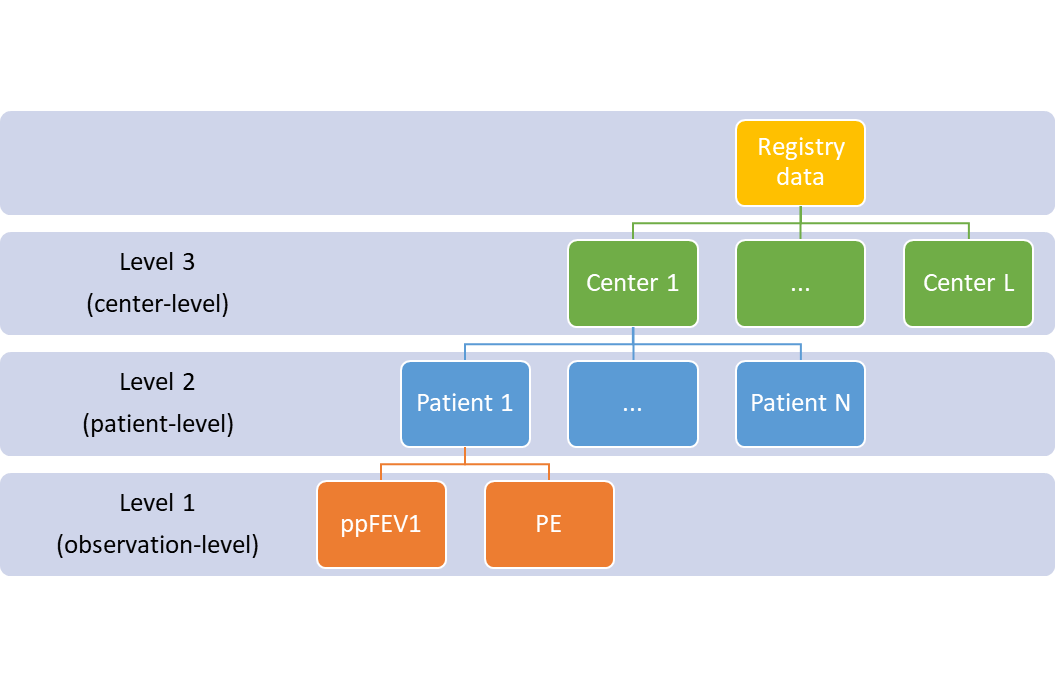
\includegraphics[width=\textwidth]{Figures/Chp1_HDS.png}
\caption{Example of the hierarchical structure of CF registry data}
\label{chp1_hds}
\end{figure}


\section{Hierarchical Model}

Throughout this dissertation, we borrow the key idea of the hierarchical (multilevel) model, allowing for observable outcomes being modeled conditionally on certain parameters, which themselves are given a probabilistic specification in terms of further parameters, known as hyperparameters. Hierarchical concept helps in understanding multiparameter problems and also plays an important role in developing computational strategies. More importantly, simple nonhierarchical models are usually inappropriate for hierarchical data. (\cite{Gelman2013a})


\subsection{Bayesian Inference}

Let $\bm{\theta}$ denote unknown parameters with $\bm{\phi}$ as the corresponding hyperparameters and $\bm{y}$ represent observed data. The key 'hierarchical' part is that $\bm{\phi}$ is unknown and thus has its own prior distribution, $p(\bm{\phi})$. The joint posterior distribution is given by 

\begin{align}
    p(\bm{\theta, \phi}|\bm{y}) & \propto p(\bm{y}|\bm{\theta,\phi})p(\bm{\theta,\phi}) \\
    & =\underbrace{p(\bm{y}|\bm{\theta})}_\text{likelihood} \underbrace{p(\bm{\theta}|\bm{\phi})}_\text{1st-stage prior} \underbrace{p(\bm{\phi})}_\text{2nd-stage prior} \nonumber
\end{align}
with the latter simplification holding because data distribution depends only on $\bm{\theta}$. The prior distribution for $\bm{\phi}$ relies on its extent of uncertainty. Either diffuse prior or (weakly) informative prior can be utilized, however, we should ensure the resulting posterior distribution is proper when using an improper prior density. More details of prior choice recommendations defer to Gelman's post(\cite{Gelman2020}). 


\subsection{Hamiltonian Monte Carlo}

Although the primary implementation is on the ubiquitous stochastic MCMC methods, in particular Metropolis-Hastings (\cite{Hastings1970}) and Gibbs sampling (\cite{Gelfand1990}), Betancourt and Girolami (\cite{Betancourt2013}) introduced a sophisticated but novel MCMC techniques, which is well known as Hamiltonian Monte Carlo (\cite{Neal2011}). It utilizes techniques from differential geometry to generate transitions spanning the full marginal variance, eliminating the random walk behavior endemic to Random Walk Metropolis and the Gibbs samplers, therefore, provides the efficient exploration for the complex hierarchical models. Detailed algorithms are not included here due to the distraction from our main purpose. Readers can refer to the Section 3 of their paper for theoretical interests.  

% The usual way to model exchangeability with covariates is through conditional independence: $p(\theta_1,\dots,\theta_j|x_1,\dots,x_J)=\int\big[\prod_{j=1}^{J}p(\theta_j|\phi,x_j)\big]p(\phi|x)d\phi$. 

% The joint prior distribution is 

% \begin{align}
%     p(\bm{\phi,\theta})=p(\bm{\theta}|\bm{\phi})p(\bm{\phi})
% \end{align}
% and the joint posterior distribtuion is 

% \begin{align}
%     p(\phi,\theta|y) & \propto p(y|\phi,\theta)p(\phi,\theta) \\
%                      & = p(y|\theta)p(\phi,\theta) \nonumber
% \end{align}

\subsection{Stan}

The inference engine Stan (not an acronym; \cite{StanManual}) releases computational constraints of Euclidean HMC. Users can build, test and run hierarchical models through this powerful probabilistic programming language for specifying the target function. Particularly, Stan adapts to No-U-Turn Sampler to preserves detailed balance by integrating not just forward in time but also backwards (\cite{Hoffman2011}). 

% overcome sensitivity to tuning parameter caused by HMC.  

In this section, we illustrate an example of hierarchical model in Stan through the combinations of two interfaces and two methods of parameterizations (centered and non-centered). Specifically, the interfaces to Stan are described as a new lightweight interface named \emph{CmdStanR}(\cite{Gabry2022}) and the conventional interface named \emph{RStan} (\cite{Rstan2020}). Note that in order to execute \emph{CmdStanR}, it is necessary to install \emph{CmdStan} first. Then we consider the Eight Schools example (\cite{Rubin1981}) in terms of the centered parameterization (\cite{Betancourt2017}), 

\begin{gather*} 
    y_n \sim N(\theta_n, \sigma_n)\\
    \theta_n \sim N(\mu, \tau)\\
    \mu \sim N(0,5) \\
    \tau \sim \mbox{Half-Cauchy}(0,5)
\end{gather*}
where $n \in \{1,\dots,8\}$ and $\{y_n, \sigma_n\}$ are given data. Secondly,  with respect to the non-centered parameterization, we introduce a latent Gaussian variable from which we can recover the group-level parameters with a scaling and a translation,

\begin{gather*} 
    y_n \sim N(\theta_n, \sigma_n)\\
    \Tilde{\theta} \sim N(0,1)\\
    \mu \sim N(0,5) \\
    \tau \sim \mbox{Half-Cauchy}(0,5)\\
    \theta_n = \mu + \tau \cdot \Tilde{\theta}
\end{gather*}

In practice, we have the same setup for the four scenarios, for instance, seed=2022, adapt\_delta=0.8, max\_treedepth=10, chains=2, warmup=1000, iters=2000. The Stan programs and R code are included in Appendix \ref{app:a}. From Figure \ref{fig:chp1_mean_tau}, we observe that resulting mean of $log(\tau)$ is strongly biased away from the true value for centered parameterization. Nonetheless, the pathology of bias and divergence is well solved by non-centered method and a thorough discussion of the non-centered intuition can be found in \cite{Betancourt2015}. It is worth noting that both interfaces are supposed to bear the same results as long as all inputs are the same. In this motivating example, we allow initial values to be unassigned so that each trajectory is distinguishable and we aim to compare elapsed time and system compatibility rather than doubting the estimates. 

Figure \ref{fig:chp1_trace_tau} shows the chains from centered parameterization (left panel) are sticking as they approaches negative values of $log(\tau)$ (or small values of $\tau$), which is indicative of the divergences. On the contrary, non-centered parameterization (right panel) stretches $log(\tau)$ further towards negative values and shows the capability to explore the neck of the funnel.

To the end, we apply the superior non-centered trick to our proposed joint models in Chapter \ref{chp2} \& \ref{chp3}. Besides, we confirm less elapsed time by interface \emph{CmdStanR}, although such advantage is not obvious in the formal example. However, when we have complicated model setups and larger sample size, the efficiency will be easily observed (see Appendix \ref{app:b}). We also note that \emph{RStan} is more compatible to windows system, while \emph{CmdStanR} is more favorable to macOS system. For applications, \emph{RStan} is utilized in Chapter \ref{chp2} while \emph{CmdStanR} is included in Chapter \ref{chp3}. To access the accuracy of posterior mean estimation, equal-tailed credible intervals are employed. Notwithstanding 95\% credible interval (CI) from \emph{RStan} is common, 90\% posterior uncertainty intervals from \emph{CmdStanr} are also recommended due to more computational stability and relation to Type-S errors (\cite{Gelman2014b}). Both intervals are incorporated in our dissertation, whilst taking account of a simulation study with $S$ replicates, we compute its corresponding 95\% confidence interval for an averaged posterior mean estimate, that is $\bar{\theta} \pm z_{0.025} * \frac{\sqrt{\sum_{s=1}^{S}(\hat{\theta}_s-\bar{\theta})^2/(S-1)}}{\sqrt{S}}$ with $\bar{\theta}=\frac{\sum_{s=1}^{S}\hat{\theta}_s}{S}$.  

%funnel of hell problem in hierarchical model
% The benefit from the non-centered parameterization is evident from Figure X. Particularly, we pick one parameter $\tau$ and transform into its logarithm $log(\tau)$. Because the logarithm allows us to better resolve behavior for small values.   

\begin{figure}[H]
\centering
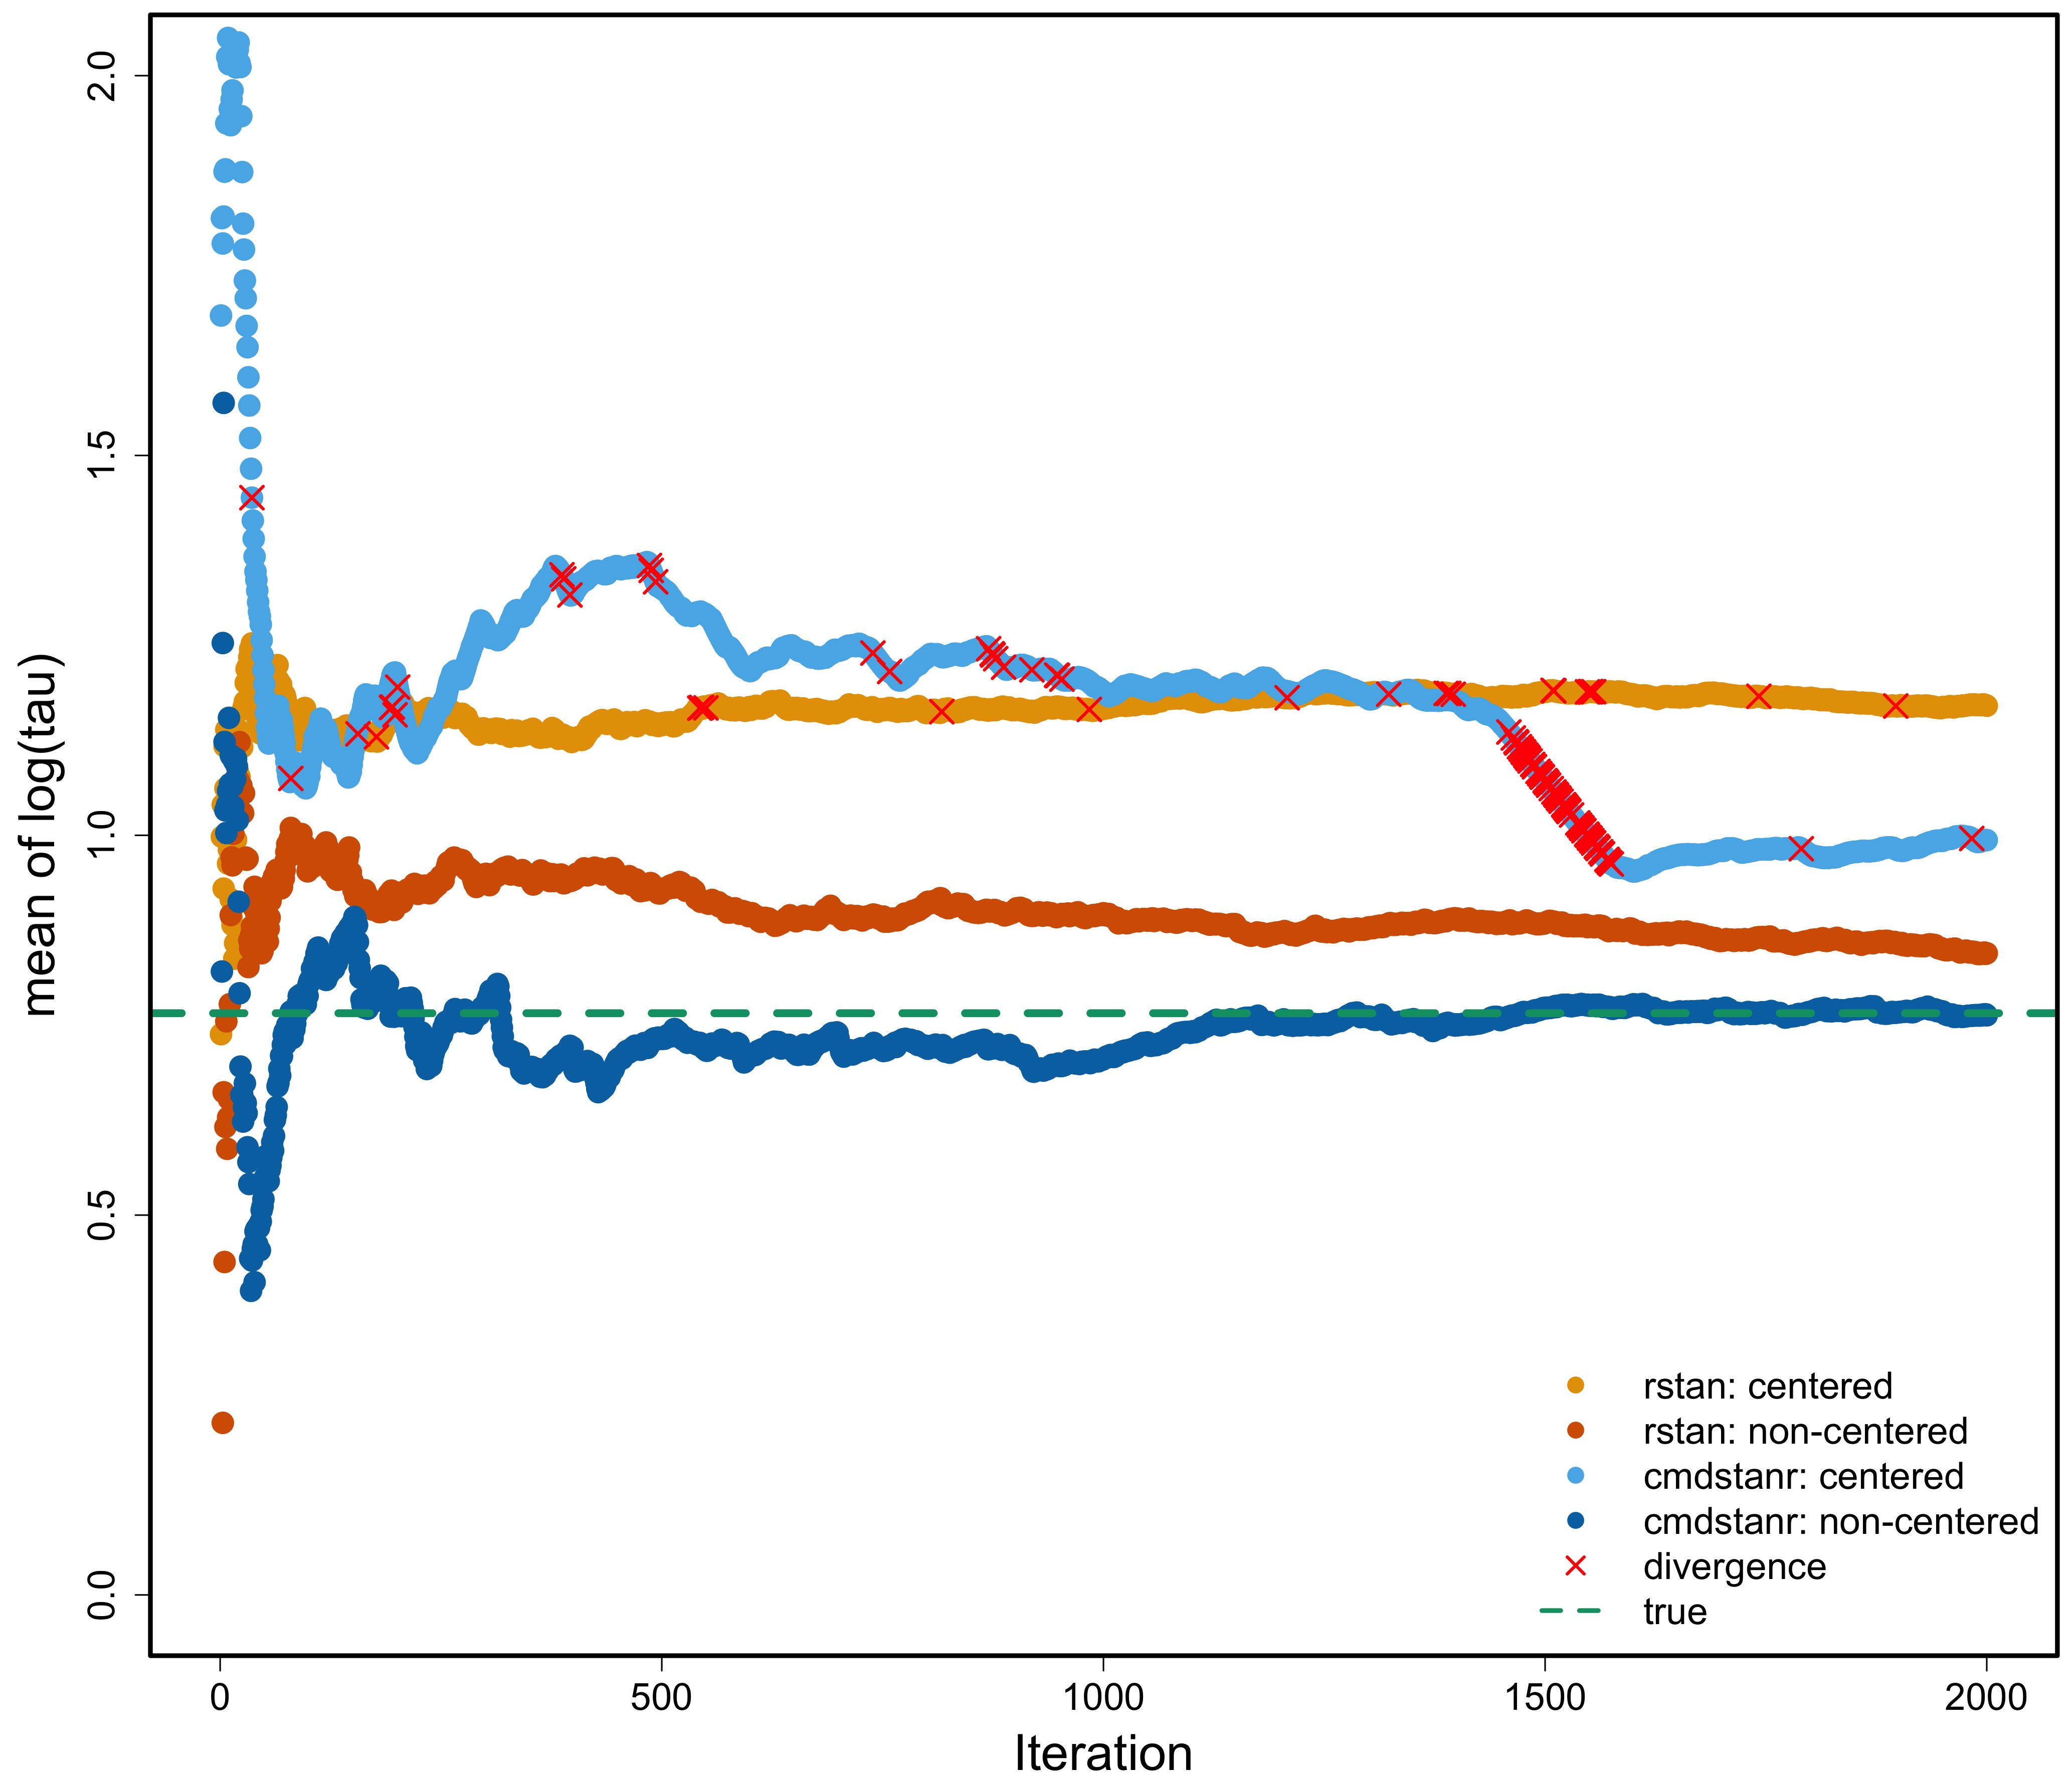
\includegraphics[width=0.9\textwidth]{Figures/Chp1_mean_tau.jpg}
\caption{Convergence of mean $log(\tau)$ towards the true expected value across four scenarios}
\label{fig:chp1_mean_tau}
\end{figure}

\begin{figure}[H]
\centering
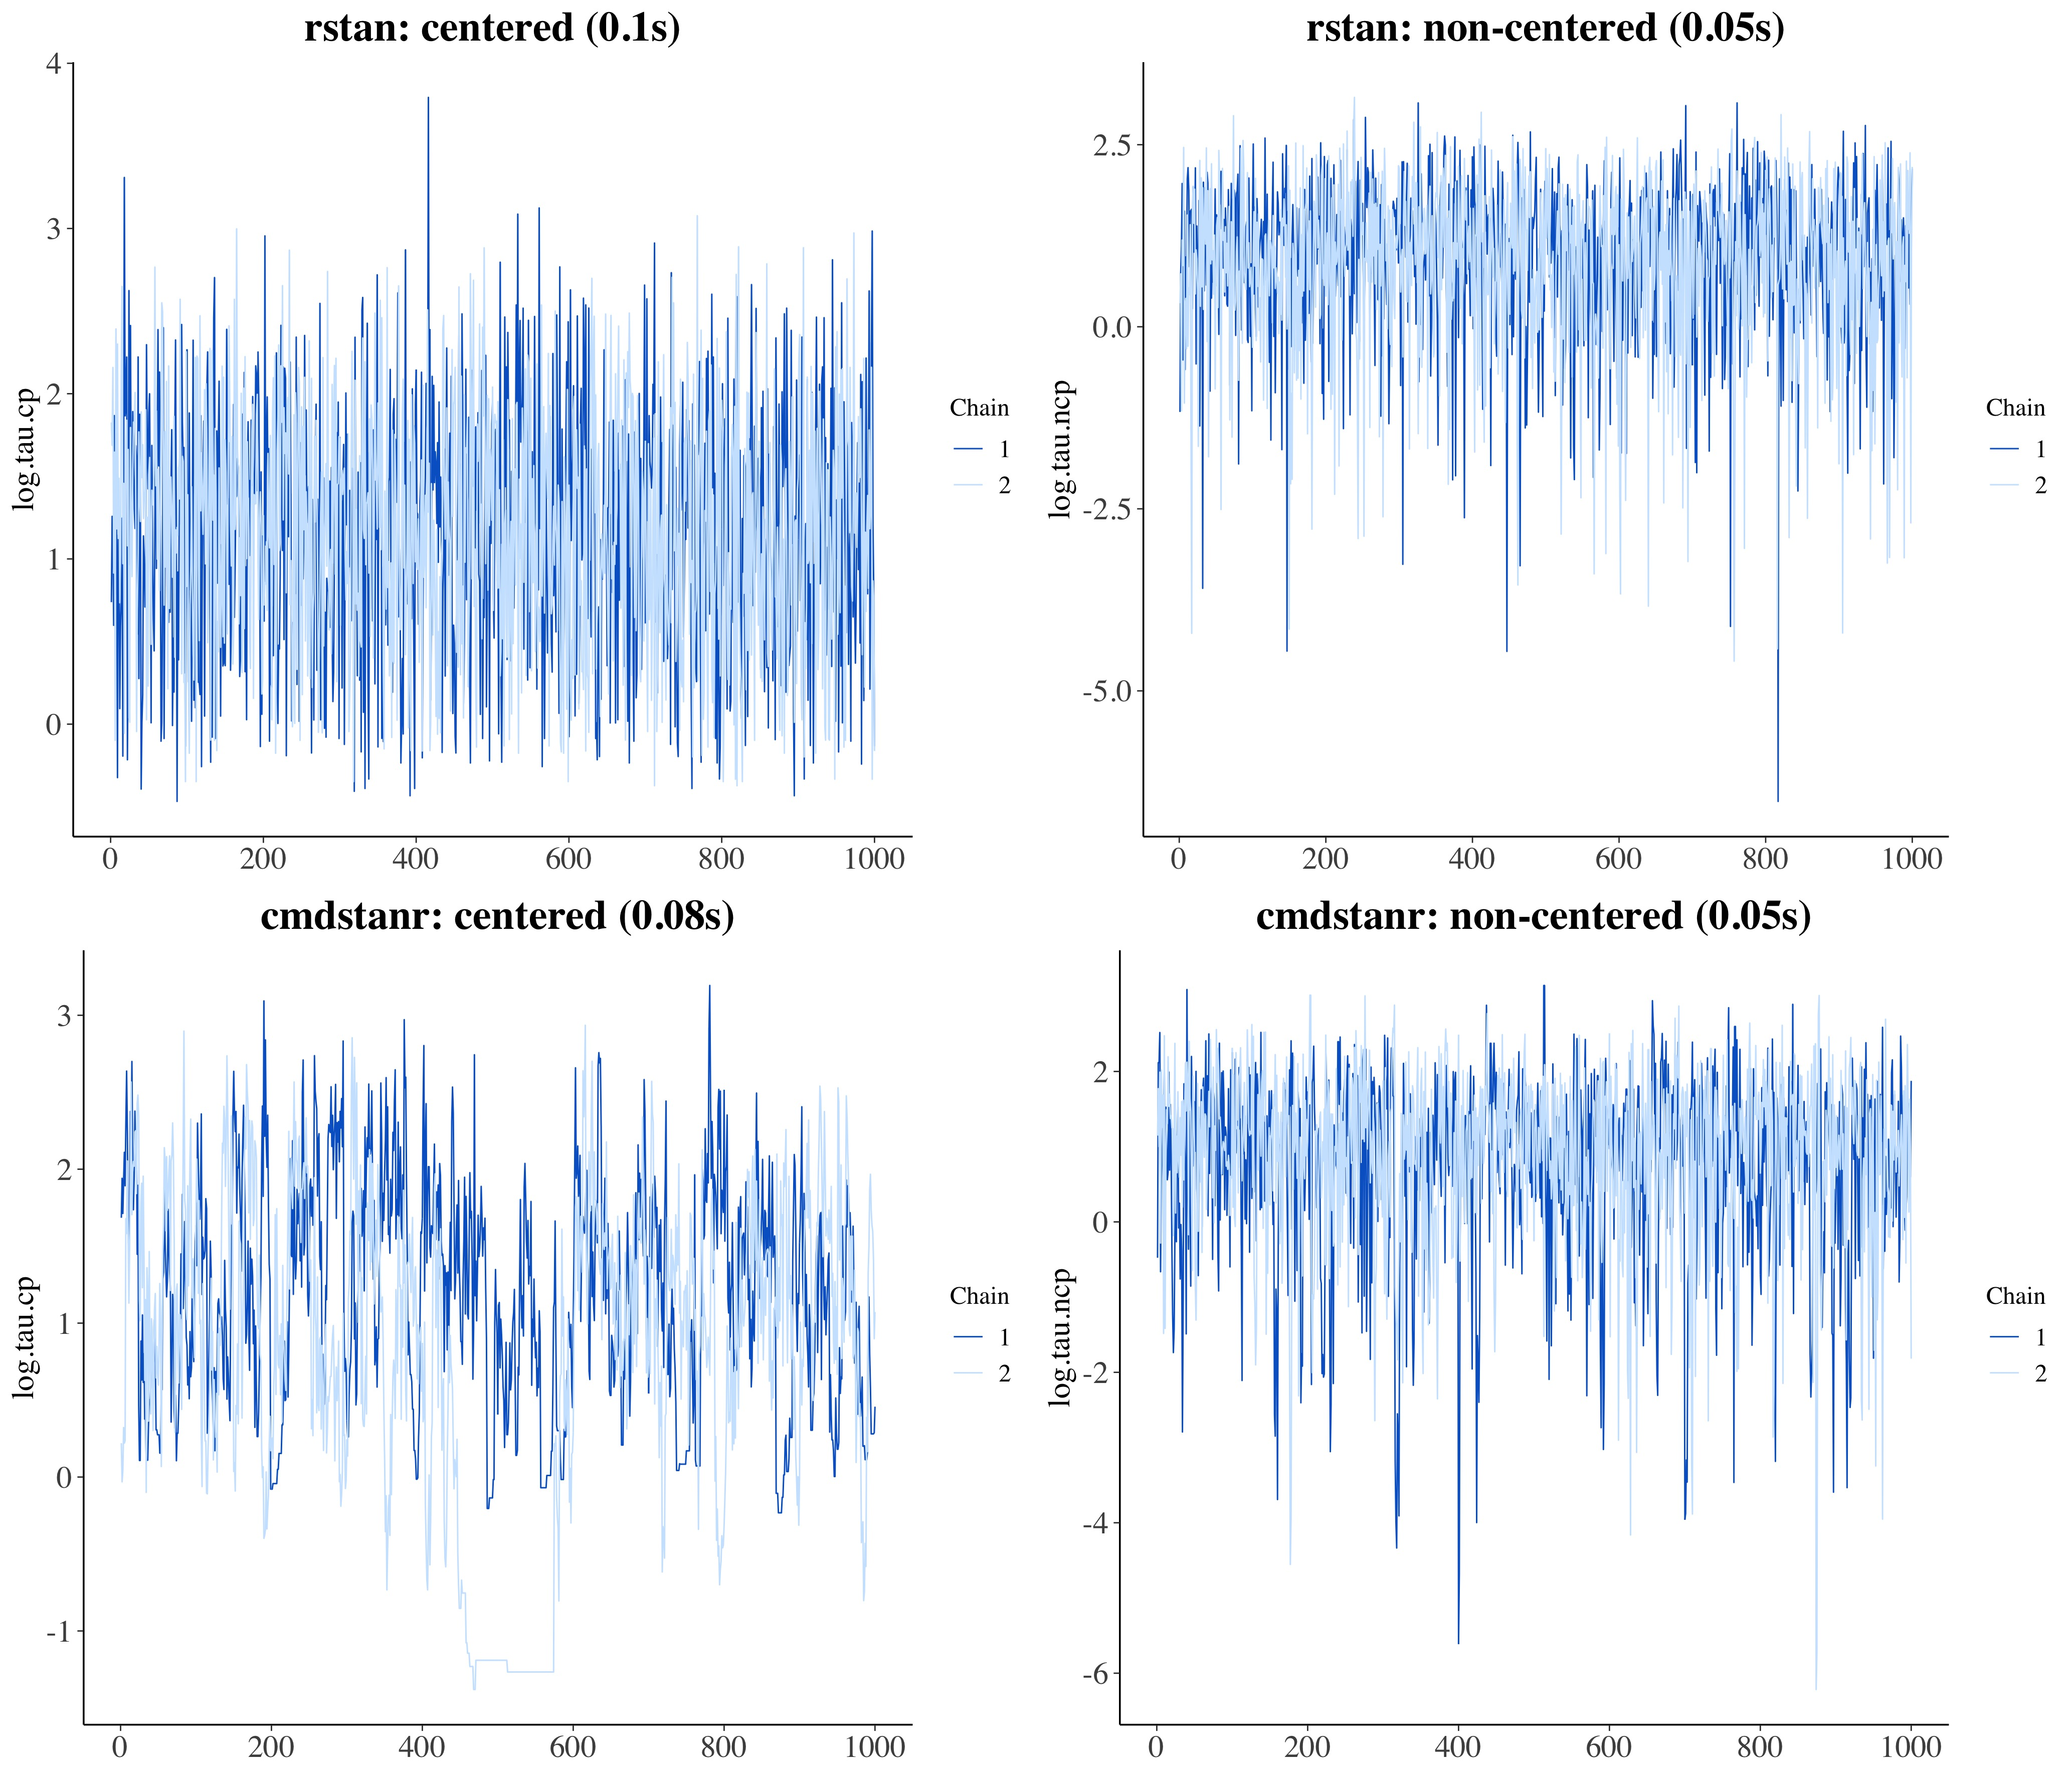
\includegraphics[width=\textwidth]{Figures/Chp1_trace_tau.jpg}
\caption{Trace plot of $log(\tau)$ across four scenarios with elapsed time in parentheses}
\label{fig:chp1_trace_tau}
\end{figure}








\chapter{Multilevel Bayesian joint model of longitudinal and binary outcomes}\label{chp2}

In this chapter, we illustrate our proposed multilevel Bayesian joint model (JM) that encompasses the Linear Mixed Effect (LME) model with a Gaussian process and the GLMM with a flexible link function. This chapter is organized as follows. In Section \ref{sec:chp2_mov}, we emphasize the motivation. In Section \ref{sec:chp2_mod}, we introduce the methodology, including model framework, Bayesian inference, predictive metrics and model comparison criterion. In Section \ref{sec:chp2_sim} and \ref{sec:chp2_app}, we illustrate simulation studies and application results, respectively. Lastly, we conclude our study with remarks and discussions in Section \ref{sec:chp2_con}. 

\section{Motivation} \label{sec:chp2_mov}

Although joint modeling has been a useful strategy in modern longitudinal analysis, applications to hierarchical longitudinal studies have been less frequent, particularly with respect to a binary process, which is commonly specified by a Generalized Linear Mixed Model (GLMM). Moreover, an added complexity occurs when the Gaussian process for irregular visits and flexible link function are involved to facilitate estimation and prediction. To the best of our knowledge, these two key challenges have not been considered together in the existing joint modeling approaches. 

For this cause, we propose a joint model that unites a LME submodel for the evolution of ppFEV1 and a GLMM for the occurrence of PE in individuals who have already experienced a PE event prior to follow up during our analysis time frame. Both center- and individual-level random intercepts are the basis of latent associations between these two submodels. In addition, we employ a stationary exponential correlation function for ppFEV1 to allow for longstanding correlation and intrinsic nonlinearity (\cite{Szczesniak2017}) and apply flexible link functions (\cite{Jiang2013}) for PE occurrence, which comprise both symmetric and asymmetric link functions to capture the underlying skewness of responses. To summarize, our motivation is threefold: i) compare common links with the flexible link; ii) quantify biases caused by ignoring center effect in a multicenter cohort analysis; iii) evaluate prognostic utility of the proposed novel joint model. 


\section{Model Framework} \label{sec:chp2_mod}

\subsection{The Joint Model}

Our proposed multilevel shared random effects joint model is expressed as 
\begin{equation} \label{eq:chp2_jm}
    \begin{gathered}
    Y_{lij}=\bm{X}_{li}(t_{lij})\bm{\alpha}+b_l+U_{li}+W_{li}(t_{lij}) + \epsilon_{lij}, \\
    Pr(R_{lij}=1)=F_{sp}\big(\bm{V}_{li}(t_{lij})\bm{\beta}+\rho_1 b_l + \rho_2 U_{li}; r_l\big)
    \end{gathered}
\end{equation}
where $Y_{lij}$ denotes continuous longitudinal profiles and $R_{lij}$ represents the binary response observed at time point $t_{lij}$ for subject $i$ from center $l$, with $l=1, \dots, L; i=1, \dots, n_l; j=1, \dots, n_{li}$. $\bm{X}_{li}(t_{lij})$ and $\bm{V}_{li}(t_{lij})$ denote row vectors of explanatory variables; $\bm{\alpha}$ and $\bm{\beta}$ are corresponding unknown coefficients. Between-center and between-patient heterogeneity are incorporated by random intercept terms $b_l$ and $U_{li}$, allowing for the assumption to be independent and identically distributed (i.i.d.) from $ N(0,\sigma_b^2)$ and $N(0,\sigma_u^2)$, respectively. A random-intercept model rather than the random intercept-and-slope model (\cite{Laird1982}) is adapted, because the latter is too rigid to capture the pattern of variability in ppFEV1 over longer periods of time \cite{TaylorRobinson2012}. The stochastic process $\bm{W}_{li}(t)$ describes how individual lung function varies over time and is assumed to be independent copies of a zero-mean, continuous-time stationary Gaussian process with the covariance function defined as 
\begin{equation}\label{eq:chp2_w}
Cov(W_{li}(t),W_{li}(s))=\tau^2 exp \big (-|t-s| \cdot \rho \big)
\end{equation}
where $t$ and $s$ are two arbitrary time points, $\rho$ represents the inverse of a range parameter and $\tau$ is the scale parameter for exponential correlation. A common concept for nugget factor $1-\mbox{nugget}=\frac{\tau^2}{\sigma^2 + \tau^2}$ incorporates both scale parameters $\tau$ and $\sigma$, with measurement error $\bm{\epsilon}$ following $N(0,\sigma^2)$. Furthermore, we assume that $\bm{b}$, $\bm{U}$ and $\bm{\epsilon}$ are mutually independent. 

Let $R_{lij}$ be a Bernoulli random variable with probability of PE occurrence $Pr(R_{lij}=1)$. $F_{sp}\big(g(\cdot); r_l\big)$ denotes a cumulative distribution function of a known symmetric power family with a linear function of covariates $g(\cdot)=\bm{V}_{li}(t_{lij})\bm{\beta}+\rho_1 b_l + \rho_2 U_{li}$ and center-specific power parameter $r_l$. Its inverse function $F^{-1}_{sp}$ is well known as a flexible symmetric power link function, which will be addressed in the next section. Parameters $\rho_1$ and $\rho_2$ measure the strength of the association through shared random components $b_l$ and $U_{li}$ between the two submodels.

\subsection{Symmetric Power Link Family}

\cite{Jiang2013} proposed a general class of power link functions, allowing flexible skewness in both positive and negative directions, while retaining the symmetric baseline link function as a special case. Let $F^{-1}_0$ be a symmetric baseline link function with corresponding cumulative distribution function (cdf) $F_0$, then symmetric power link family is defined as

\begin{equation} \label{eq:ch2_Fsp}
  F_{sp}(x;r)=F_0^r(\frac{x}{r})I_{(0,1]}(r)+\big[1-F^{1/r}_0(-rx)\big]I_{(1,+\infty)}(r),    
\end{equation}
where $I_A(r)$ is an indicator function with 1, when $r \in A$ and 0, otherwise. $x \in (-\infty, +\infty)$ denotes the linear function of predictors and $r$ is called by power parameter. The inverse transformation $x=F^{-1}_{sp}(\pi)$ is well known as the symmetric power link with $\pi \in [0,1]$. However, we are in favor of $F_{sp}$ because the probability of event occurrence $Pr(R_{lij}=1)=F_{sp}\big(g(\cdot);r_l\big)$. Particularly, $F_{sp}$ becomes cdf of splogit link when $F_0$ follows a Logistic distribution with location=0 and scale=1, and the cdf of spep link when $F_0$ follows a Laplace distribution location=0 and scale=1, as shown in Equation \ref{eq:F0}. 

\begin{align}
& F_0= \left \{\begin{array}{ll}
  F_{\mbox{logistic}}(x|\mu=0, s=1)= \frac{1}{1+exp(-x)}\\
  F_{\mbox{laplace}}(x|\mu=0, b=1)=\frac{exp(x)}{2}I_{(-\infty,0)}(x)+\big(1-\frac{exp(x)}{2}\big)I_{[0, +\infty)}(x)
\end{array}\right.
\label{eq:F0}
\end{align}

Figure \ref{fig:Chp2_cdf_sp} illustrates the skewness of response probability given covariate $x$ is symmetric about zero. Particularly, splogit reduces to the logit link when power parameter $r=1$ and we observe that spep link provides flexible range of skewness and adjustment of tail behavior as addressed in \cite{Jiang2013}. 

\begin{figure}[H]
\centering
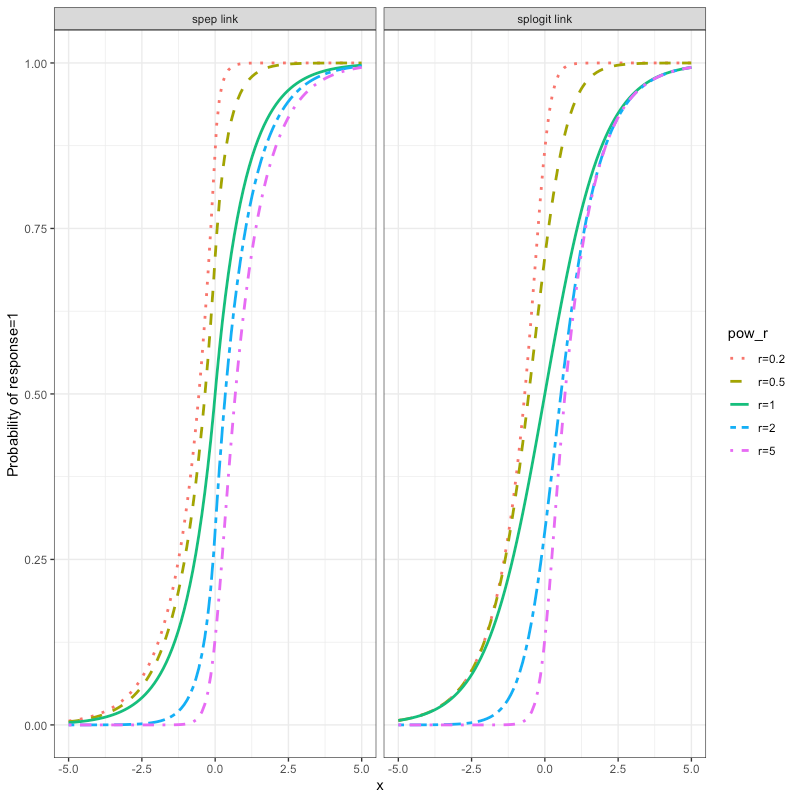
\includegraphics[width=0.9\textwidth]{Figures/Chp2_cdf_sp.png}
\caption{Plot for $F_{\mbox{splogit}}$ and $F_{\mbox{spep}}$}
\label{fig:Chp2_cdf_sp}
\end{figure}

\subsection{Prior Specifications and Posterior Inference}\label{sec:chp2_prior}

For all unknown parameters, we assume the following prior distributions: 1) regression coefficients $(\bm{\alpha}^T, \bm{\beta}^T$): non-informative multivariate normal priors with mean $\bm{0}$ and a large variance; 2) scale parameters $(\sigma_b,\sigma_u,\sigma)$: weakly informative proper priors with half Cauchy distribution \cite{Gelman2006}; 3) correlation scale parameter $\tau$: a truncated normal distribution; 4) correlation length-scale parameter $\rho$: a diffuse inverse gamma prior; 5) power parameters $\bm{r}^T$: gamma distributions \cite{Jiang2013}$,$ \cite{Upadhyay2015}; 6) association parameters $(\rho_1, \rho_2)$: uniform priors. Explicit values of hyperparameters are included in Appendix \ref{app:b}.

Let $\bm{\Psi}=(\bm{\alpha}^T, \bm{\beta}^T, \bm{r}^T,\sigma_b,\sigma_u,\sigma,\tau,\rho,\rho_1,\rho_2)$, $\bm{D}_{obs}=(\bm{Y}_{li},\bm{R}_{li})^T$, the joint posterior distribution of $(\bm{\Psi},\bm{b},\bm{U},\bm{W})$ is written as 

\begin{equation}
\begin{split}
\pi(\bm{\Psi},\bm{b},\bm{U},\bm{W}|\bm{D}_{obs}) \propto &
  \pi(\bm{D}_{obs},\bm{b},\bm{U},\bm{W}|\bm{\Psi}) \pi(\bm{\Psi}) \\
\propto & \pi(\bm{D}_{obs}|\bm{b},\bm{U},\bm{W},\bm{\Psi}) \pi(\bm{b}|\bm{U},\bm{W},\bm{\Psi})\pi(\bm{U}|\bm{W},\bm{\Psi}) \pi(\bm{W}|\bm{\Psi})\pi(\bm{\Psi}) \\ 
 \propto & \pi(\bm{Y},\bm{R}|\bm{b},\bm{U},\bm{W},\bm{\Psi}) \pi(\bm{b}|\bm{\Psi}) \pi(\bm{U}|\bm{\Psi}) \pi(\bm{W}|\bm{\Psi}) \pi(\bm{\Psi}) \\
 \propto & \prod_{l=1}^{L}\prod_{i=1}^{n_l}I(\bm{Y}_{li},\bm{R}_{li}|b_{l}, U_{li}, \bm{W}_{li}, \bm{\Psi}) \pi(b_l|\sigma_b) \pi(U_{li}|\sigma_u) \pi(\bm{W}_{li}|\tau,\rho) \pi(\bm{\Psi})
\end{split}
\end{equation}
where the likelihood function $\bm{I}(\bm{Y}_{li},\bm{R}_{li}|b_l,U_{li},\bm{W}_{li},\bm{\Psi})= \bm{I}_1(\bm{Y}_{li}|b_l,U_{li},\bm{W}_{li},\bm{\Psi}) \bm{I}_2(\bm{R}_{li}|b_l,U_{li},\bm{\Psi})$ by the assumption of conditional independence between $\bm{Y}$ and $\bm{R}$ given random effects $\bm{b}$ and $\bm{U}$. We further suppress the dependence of each component in $\bm{\Psi}$.

% All posterior samplings are carried out through HMC by R interface to Stan, namely RStan \cite{Rstan2020}.

\subsection{Dynamic Individual Prediction} \label{sec:chp2_pred}

We employ the best linear unbiased predictor (BLUP) to predict individual random intercept $U_{li'}$ and time-continuous random variable $\bm{W}_{li'}(t)$ for any new patient $i'$ from the existing center $l$. The explicit forms are obtained by the properties of the multivariate normal distribution as utilized in \cite{Diggle2015} as 

\begin{align}
    E\big(U_{li'}|\bm{Y}_{li'},b_l, \bm{\phi},\bm{\alpha}\big)  = & \sigma_u^2\bm{K}^T_{li'}\big(\bm{V}_{li'}(\bm{\phi})\big)^{-1} (\bm{Y}_{li'}-\bm{X}_{li'}\bm{\alpha}-b_l\bm{K}_{li'})\label{chp2:eq4} \\
    E\big(W_{li'}(t_{li'j}\big)|\bm{Y}_{li'},b_l, \bm{\phi},\bm{\alpha})  =  & \tau^2\bm{F}^{j^T}_{li'}\big(\bm{V}^j_{li'}(\bm{\phi})\big)^{-1}  (\bm{Y}^j_{li'}-\bm{X}^{j}_{li'}\bm{\alpha}-b_l\bm{K}^j_{li'}) \label{chp2:eq5}
\end{align}
where $\bm{Y}_{li'}$ and $\bm{X}_{li'}$ are observed data and covariates, respectively. $\bm{K}_{li'}$ denotes an $n_{li'} \times 1$ matrix of ones and $\bm{\alpha}$ is as before. Also,
 
 \begin{equation}
    \bm{V}_{li'}(\bm{\phi})=\sigma_u^2\bm{J}_{li'}+\tau^2\bm{R}_{li'}+\sigma^2\bm{I}_{li'}
 \end{equation} 
 where $\bm{\phi}=(\sigma^2_2,\tau^2,\sigma^2,\rho)$, $\bm{J}_{li'}$ is an $n_{li'} \times n_{li'}$ matrix of ones, $\bm{R}_{li'}$ is an $n_{li'} \times n_{li'}$ matrix with $(t,t')th$ element $exp(-|t-t'| \cdot \rho)$ and $\bm{I}_{li'}$ is an $n_{li'} \times n_{li'}$ identity matrix.
 
 Let response and covariates history up to an observed time point $j$ be presented by $\bm{Y}_{li'}^j$ and  $\bm{X}_{li'}^j$ in Equation (\ref{chp2:eq5}). $\bm{F}^j_{li'}=\Big(exp(-|t_{li'1}-t_{li'j}| \cdot \rho), \dots, exp(-|t_{li'j}-t_{li'j}| \cdot \rho) \Big)^T$, $\bm{V}^j_{li'}$ is the variance-covariance matrix of $\bm{Y}^j_{li'}$. Analogously, forecasting $W_{lij'}$ at time $t_{lij}$ with lead-time $u$ for an existing patient $i$ is obtained by 
 \begin{equation}
  E\big(W_{li}(t_{lij}+u)|\bm{Y}^j_{li},b_l, U_{li},\bm{\phi}, \bm{\alpha}\big)  =  \tau^2\bm{F}^{{j,u}^T}_{li}\big(\bm{G}^j_{li}(\bm{\phi})\big)^{-1}(\bm{Y}^j_{li}-\bm{X}^{j}_{li}\bm{\alpha}-b_l\bm{K}^j_{li}-U_{li}\bm{K}^j_{li}) \label{chp2:eq6}
\end{equation}
where $\bm{G}^j_{li}(\bm{\phi})=\tau^2\bm{R}^j_{li}+\sigma^2\bm{I}^j_{li}$, $\bm{R}^j_{li}$ and $\bm{I}^j_{li}$ are as before but with new dimensions of $j \times j$. $\bm{F}^{j,u}_{li}=\Big(exp(-|t_{lij}+u-t_{li1}| \cdot \rho),\dots,exp(-|t_{lij}+u-t_{lij}| \cdot \rho) \Big)^T$. Whenever a new response at time $t_{lij'}$ becomes available, the prediction from Equation (\ref{chp2:eq6}) will be dynamically updated. 
In the real data study, we apply empirical BLUPs to achieve the prognosis for ppFEV1 and PE according to Equation \ref{eq:chp2_jm}. 

% \begin{align*}
% & \mbox{Predict for new patients} \left \{\begin{array}{ll}
%  E({Y}_{li'j}) = \bm{X}_{li'}(t_{li'j})\widehat{\bm{\alpha}}+\widehat{\rho}_1\widehat{b}_l+\widehat{\rho}_2\widehat{U}_{li'}+\widehat{W}_{li'}(t_{li'j})\\
%  Pr(R_{li'j}=1) = F_{sp}\big(\bm{V}_{li}(t_{li'j})\widehat{\bm{\beta}}+\widehat{\rho}_1\widehat{b}_l+\hat{\rho}_2\widehat{U}_{li'};\widehat{r}_l\big)
% \end{array}\right. \\\\
% & \mbox{Forecast for existing patients} \left \{\begin{array}{ll}
%  E({Y}_{lij'})  = \bm{X}_{li}(t_{lij'})\widehat{\bm{\alpha}}+\widehat{\rho}_1\widehat{b}_l+\widehat{\rho}_2\widehat{U}_{li}+\widehat{W}_{li}(t_{lij'})\\
%  Pr(R_{lij'}=1)  = F_{sp}\big(\bm{V}_{li}(t_{lij'})\widehat{\bm{\beta}}+\widehat{\rho}_1\widehat{b}_l+\widehat{\rho}_2\widehat{U}_{li};\widehat{r}_l\big)
% \end{array}\right.
% \end{align*}

\subsection{Model Selection}

In this section we consider a recent measure of comparison between models. The Watanabe-Akaike information criterion (WAIC) \cite{Watanabe2010} is favored as a full Bayesian approach for estimating the out-of-sample expectation, by averaging over the posterior distribution rather than conditioning on a point estimate, thus is invariant to reparameterisations contrary to the Deviance Information Criterion (DIC) \cite{Spiegelhalter2002}. In a comprehensive review paper, Gelman and his colleagues \cite{Gelman2014} recommended expression on the deviance scale in terms of variance adjustment, written as

\begin{equation}
    \begin{split}
    \mbox{WAIC}=-2\Big \{\sum_{i=1}^{n}log\big(p_{post}(y_i|\theta)\big)-\sum_{i=1}^{n}\mbox{var} \Big (log\big( p_{post}(y_i|\theta)\big) \Big ) \Big \}
    \end{split}
\end{equation}

Computed $\mbox{WAIC}_1$ and $\mbox{WAIC}_2$ for the two submodels are defined as follows

\begin{align}
  & \widehat{\mbox{WAIC}}_1=-2\Big \{\sum^{L}_{l=1}\sum^{n_l}_{i=1}\sum^{n_{li}}_{j=1}\Big ( log\big [\frac{1}{S}\sum_{s=1}^S \bm{I}_1(Y_{lij}|b^s_l,U^s_{li},W^s_{lij},\bm{\Psi}^s)\big] - V_{s=1}^{S}log\big[\bm{I}_1(Y_{lij}|b^s_l,U^s_{li},W^s_{lij}, \bm{\Psi}^s)\big] \Big ) \Big \} \label{eq:waic1}\\   
  & \widehat{\mbox{WAIC}}_2=-2\Big \{\sum^{L}_{l=1}\sum^{n_l}_{i=1}\sum^{n_{li}}_{j=1}\Big (log\big [\frac{1}{S}\sum_{s=1}^S \bm{I}_2(R_{lij}|b^s_l,U^s_{li},\bm{\Psi}^s)\big] -  V_{s=1}^{S}log\big[\bm{I}_2(R_{lij}|b^s_l,U^s_{li}, \bm{\Psi}^s)\big] \Big ) \Big \}  \label{eq:waic2}
\end{align}
where $\bm{I}_1$ and $\bm{I}_2$ denote the likelihood function for normal distribution and bernoulli distribution, respectively. $S$ is the number of simulation draws, $\bm{\Psi}^s$ is the vector of the model parameters at $s^{th}$ iteration. $V_{s=1}^S$ represents the sample variance, that is $V_{s=1}^S\bm{a}=\frac{1}{S-1}\Sigma^{S}_{s=1}(a_s-\bar{a})^2$. Practically, calculations on Equation (\ref{eq:waic1}) and (\ref{eq:waic2}) could be easily achieved by the \emph{waic} function from the \emph{loo} package (v2.3.1) \cite{Vehtari2020} by extracting pointwise log-likelihood values from the posterior samplings. The model with the smaller WAIC indicates the better goodness of fit. 

\section{Simulated Examples} \label{sec:chp2_sim}

\subsection{Simulation Study A}

The first simulation study is designed to explore the flexibility of splogit in comparison with three common links, namely logit, probit, cloglog. Hereafter, we name them by the rule of link-JM. The explicit expressions are shown as

\begin{align}
& \left \{\begin{array}{ll}
  F_{\mbox{splogit}}(x)= [1+exp(\frac{x}{r})]^{-r}I_{(0,1]}(r)+\big\{1-[1+exp(-rx)]^{-\frac{1}{r}}\big\} I_{(1,+\infty)}(r)\\ 
  F_{\mbox{logit}}(x)= [1+exp(x)]^{-1}\\ 
  F_{\mbox{probit}}(x)= \Phi(x), \mbox{where $\Phi$ is the cdf of standard normal }\\ 
  F_{\mbox{cloglog}}(x)= 1-e^{-e^x}
\end{array}\right.
\end{align}
Then we simulate multicenter data sets with proposed splogit-JM to fit following joint models, of the forms

\begin{align*}
\mbox{logit-JM} & \left \{\begin{array}{ll}
        Y_{lij}= \alpha_0 + x_{li1}\alpha_1 + x_{li2}\alpha_2 + b_l + U_{li} + \epsilon_{lij} \\
       \mbox{Pr}(R_{lij}=1)=F_{\mbox{logit}}(\beta_0 + \beta_1 t_{lij} + \rho_1 b_l + \rho_2 U_{li}) \\
\end{array}\right. \\
\mbox{probit-JM} & \left \{\begin{array}{ll}
       Y_{lij}= \alpha_0 + x_{li1}\alpha_1 + x_{li2}\alpha_1+b_l+U_{li} + \epsilon_{lij} \\
       \mbox{Pr}(R_{lij}=1)=F_{\mbox{probit}}(\beta_0 + \beta_1 t_{lij} +\rho_1 b_l + \rho_2 U_{li}) \\
\end{array}\right. \\
\mbox{cloglog-JM} & \left \{\begin{array}{ll}
       Y_{lij}= \alpha_0 + x_{li1}\alpha_1 + x_{li2}\alpha_1+b_l+U_{li} + \epsilon_{lij} \\
       \mbox{Pr}(R_{lij}=1)=F_{\mbox{cloglog}}(\beta_0 + \beta_1 t_{lij} + \rho_1 b_l + \rho_2 U_{li}) \\
        \end{array}\right.\\
\mbox{splogit-JM} & \left \{\begin{array}{ll}
       Y_{lij}= \alpha_0 + x_{li1}\alpha_1 + x_{li2}\alpha_1+b_l+U_{li} + \epsilon_{lij} \\
       \mbox{Pr}(R_{lij}=1)=F_{\mbox{splogit}}(\beta_0 + \beta_1 t_{lij} + \rho_1 b_l + \rho_2 U_{li};r_l) \\
       \end{array}\right.        
\end{align*}
where all the notations are as before. Without loss of generality, we simulate a balanced data set, that is $L=5,n_l=50, n_{li}=5$ for 50 replicates. Moreover, we set regression coefficients $\alpha_0=1, \alpha_1=-3, \alpha_2=0.7, \beta_0=0.5, \beta_1=4$, power parameter $\bm{r}=(0.2, 0.5, 1, 2, 3)^T$ and association parameters $\rho_1=0.5, \rho_2=0.8$. Let $x_{li1} \sim N(0,1), x_{li2} \sim \mbox{Bernoulli}(0.5), b_l \sim N(0,\sigma^2_b), U_{li} \sim N(0,\sigma^2_u)$ and $\epsilon_{lij} \sim N(0, \sigma^2)$, with $\sigma_b=5, \sigma_u=3, \sigma=0.45$. Time point $t_{lij}$ is simulated from a uniform(0,6) distribution by assuming every patient starts from time=0 and is standardized to ensure the computational stability.  

All models are estimated by HMC with 4000 post-warmup iterations via two chains. Averaged results and model information criterion are summarized in Figure \ref{fig:chp2_sima} and Table \ref{tab:chp2_sima}, respectively. Posterior samplings are ensured to converge until all values for the potential scale reduction factor $\hat{R}$ are below 1.1 (\cite{Gelman1992}). All other details can be found in Appendix \ref{app:b}. 

\begin{center}
\begin{table}[H]
\caption{Comparison of logit-, probit-, cloglog- and splogit-JM over simulated data sets for 50 replicates}
\label{tab:chp2_sima}
 \centering
 \begin{threeparttable}
  \begin{tabular}{m{0.2\textwidth}m{0.2\textwidth}m{0.2\textwidth}m{0.2\textwidth}}
  \toprule
 Fitted Model & $\mbox{WAIC}$ \tnote{a} \hspace*{1.8mm} & $\mbox{WAIC}_1$ \tnote{b}  \hspace*{1.8mm}  & $\mbox{WAIC}_2$ \tnote{c}  \hspace*{1.8mm}\\
 \midrule
   logit-JM & 2239.93 & 1807.16 & 432.77 \\
  
   probit-JM & 2244.44 & 1807.49 & 436.95 \\
  
   cloglog-JM & 2272.57  & 1808.24 & 464.33 \\
   
   \bf splogit-JM & 2203.00 & 1806.37 & 396.63 \\
    \bottomrule
  \end{tabular}
   \begin{tablenotes}[para]
    \footnotesize
    Note: model in boldface: true model; \item[a] Joint model; \item[b] Continuous submodel; \item[c] Binary submodel
    \end{tablenotes}
    \end{threeparttable}
\end{table}
\end{center}

\begin{figure}[H]
\centering
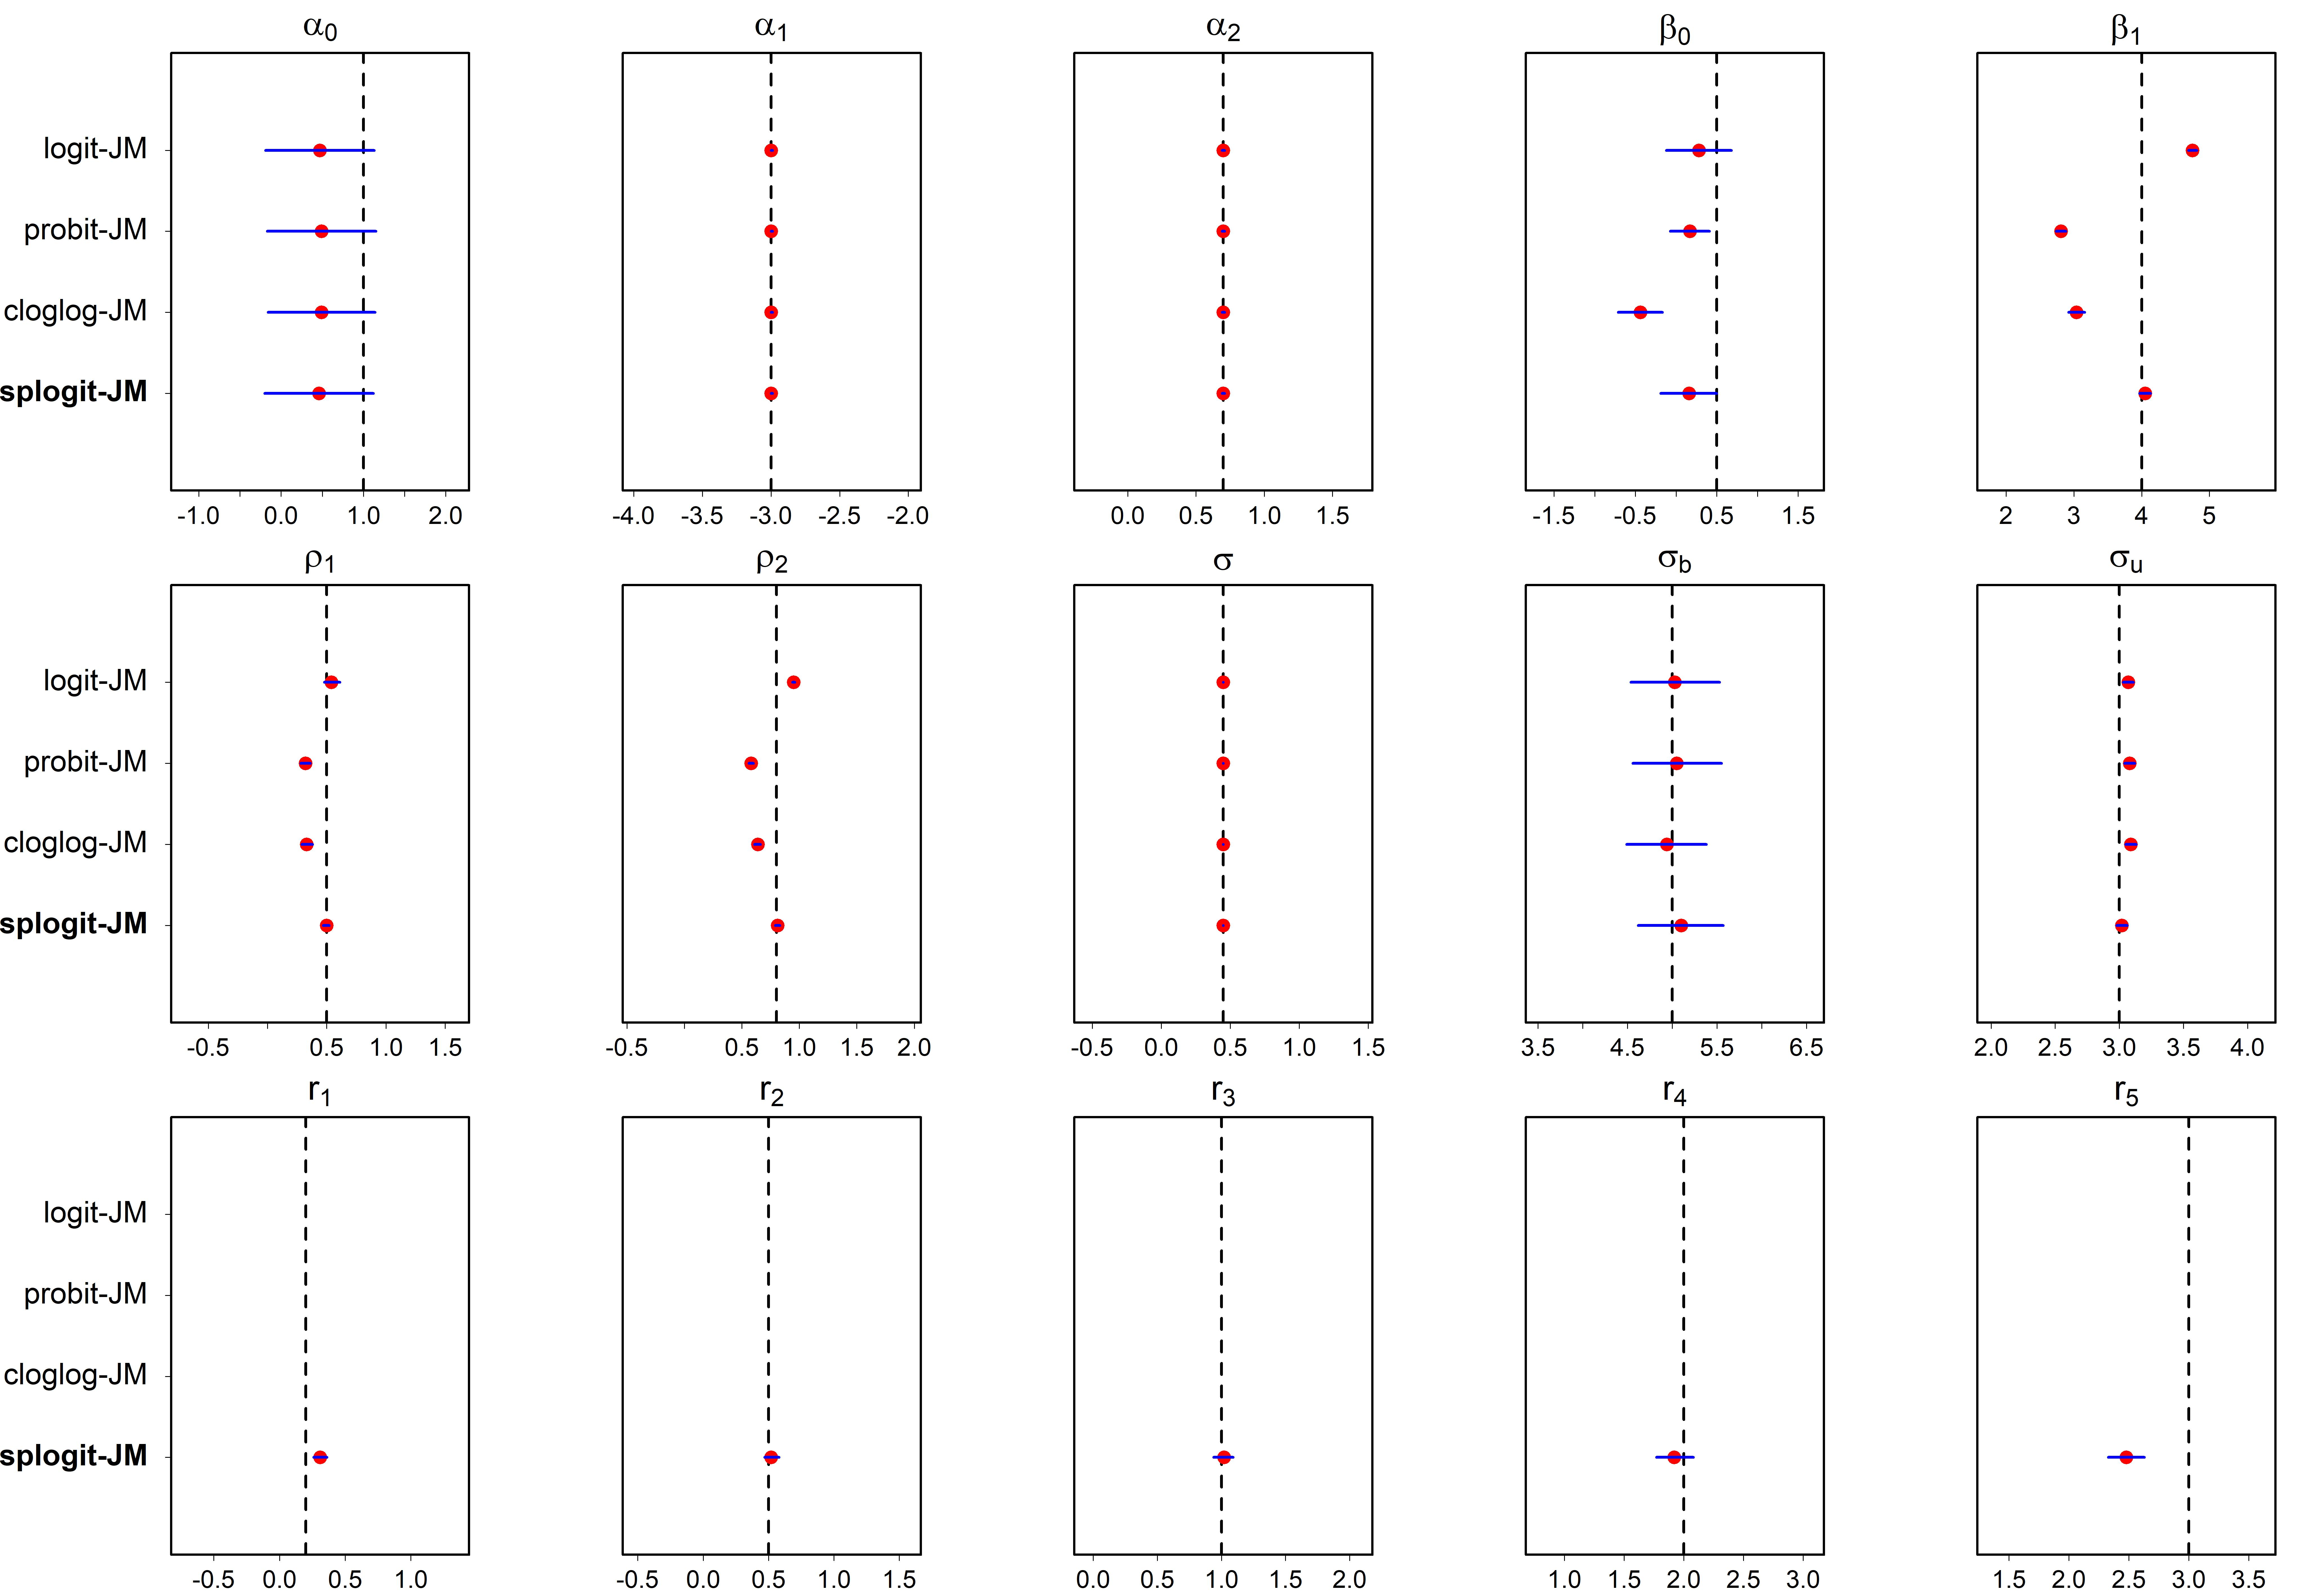
\includegraphics[width=\textwidth]{Figures/Chp2_SIM_SPLOGIT_A.jpg}
\caption{Averaged posterior means by 50 replicates via CmdStanr with true model (boldface), true value (dashed vertical line), posterior mean estimates (red dot) and corresponding 95\% confidence interval (blue line).}
\label{fig:chp2_sima}
\end{figure}

Table \ref{tab:chp2_sima} demonstrates that center-specific power parameter induces great flexibility than common fixed links in a hierarchical data structure by the smallest $\mbox{WAIC}_2$. Among those conventional links, logit-JM as the special case of true splogit-JM outperforms others. Figure \ref{fig:chp2_sima} shows the reasonable performance in recovering the true values (especially $\sigma_b$) and we concur that estimates for $\alpha_0$ and $r_5$ can be further improved with more iterations or sample size or replicates.   

\subsection{Simulation Study B} 

In this section, we implement another simulation study to explore the performance of JM under eight scenarios (four JMs $\times$ two flexible links). We take the LME submodel without fixed effects for simplicity purpose and JM equations are specified as follows 
\begin{align*}
& \mbox{JM}_1 \left \{\begin{array}{ll}
        Y_{lij}= U_{li} + \epsilon_{lij} \\
       \mbox{Pr}(R_{lij}=1)=F_{sp}(\beta_0+\beta_1t_{lij}+ \rho_2 U_{li};r) \\
\end{array}\right. \\
& \mbox{JM}_2 \left \{\begin{array}{ll}
        Y_{lij}=b_l + U_{li} + \epsilon_{lij}\\
       \mbox{Pr}(R_{lij}=1)=F_{sp}(\beta_0+\beta_1t_{lij}+\rho_1 b_l + \rho_2 U_{li};r) \\
\end{array}\right. \\
&\mbox{JM}_3 \left \{\begin{array}{ll}
       Y_{lij}=b_l + U_{li} + \epsilon_{lij} \\
       \mbox{Pr}(R_{lij}=1)=F_{sp}(\beta_0+\beta_1t_{lij}+\rho_1 b_l + \rho_2 U_{li};r_l) \\
        \end{array}\right.\\
&\mbox{JM}_4 \left \{\begin{array}{ll}
        Y_{lij}=b_l + U_{li} + W_{lij} + \epsilon_{lij} \\
       \mbox{Pr}(R_{lij}=1)=F_{sp}(\beta_0+\beta_1t_{lij}+\rho_1 b_l + \rho_2 U_{li};r_l) \\
       \end{array}\right.        
\end{align*}
where $\mbox{JM}_1$ is designed as a misspecified model and $\mbox{JM}_4$ is the proposed model with exponential correlation and center-specific power parameter; $t_{lij}$ is a standardized age variable for the stabilization of posterior computations. We set regression coefficients $\beta_0=0.5$, $\beta_1=4$ and association parameters $\rho_1=0.5$, $\rho_2=0.8$. Let $b_l \sim N(0,\sigma^2_b)$, $U_{li} \sim N(0,\sigma^2_u)$ and $\epsilon_{lij} \sim N(0,\sigma^2)$, with $l=1, \dots,5, i=1, \dots, 50, j=1, \dots, 10, \sigma_b=5, \sigma_u=3, \sigma=0.45$; $W_{li}(\bm{t})$ be the stationary Gaussian process with $\tau=1.5$ and $\rho=0.5$ as defined in Section \ref{eq:chp2_w}. We simulate a total of 100 data sets (50 for splogit-$\mbox{JM}_4$ and 50 for spep-$\mbox{JM}_4$) under true power parameters $\bm{r}=(0.2, 0.5, 1, 1, 2)^T$. Priors are defined according to Section \ref{sec:chp2_prior}. All models are estimated by HMC with at least 10,000 iterations via two chains. The first 4000 draws are discarded as a warm-up sampling and every third values are kept for the posterior inference. We ensure all results satisfy the convergence diagnostic $\hat{R}$.

\begin{center}
\begin{table}[ht]
\caption{Model comparisons over simulated data sets for 50 replicates} \label{tab:chp2_sim}
 \centering
 \begin{threeparttable}
  \begin{tabular}{lllllll}
    \toprule
   & \multicolumn{6}{c} {True Model}\\
    \cmidrule(lr) {2-7} 
  Fitted Model & \multicolumn{3}{c}{splogit-$\mbox{JM}_4$} & \multicolumn{3}{c}{spep-$\mbox{JM}_4$}  \\
 \cmidrule(lr) {2-4}  \cmidrule(lr) {5-7}
 & $\mbox{WAIC} \tnote{a} $ & $\mbox{WAIC}_1 \tnote{b}$  & $\mbox{WAIC}_2 \tnote{c}$  &
 $\mbox{WAIC} \tnote{a}$ & $\mbox{WAIC}_1 \tnote{b}$ & $\mbox{WAIC}_2 \tnote{c}$ \\
 \midrule 
   Misspecified ($\mbox{JM}_1$) & 9455.853 & 8369.268 & 1086.585 &
                9256.9877 & 8299.09 & 957.8977 \\
  
   No center-index ($\mbox{JM}_2$) & 9362.319 & 8360.999 & 1001.32 &
                9179.9247 &  8292.143 &  887.7817 \\
  
   No covariance ($\mbox{JM}_3$) &  9328.3859 & 8360.075 & 968.3109 &
                 9157.4637 & 8291.87 &  865.5937 \\
   
   \textbf{Proposed ($\mbox{JM}_4$)} & \textbf{8508.9091} & \textbf{7574.098} & \textbf{934.8111} & \textbf{8352.8335} & \textbf{7541.872} & \textbf{810.9615} \\
    \bottomrule
  \end{tabular}
   \begin{tablenotes}[para]
    \footnotesize
        Note: model in boldface: true model; value in boldface: the smallest value; \item[a] Joint model; \item[b] Continuous submodel; \item[c] Binary submodel
    \end{tablenotes}
    \end{threeparttable}
\end {table}
\end{center}

As shown in Table \ref{tab:chp2_sim}, both splogit-$\mbox{JM}_4$ and spep-$\mbox{JM}_4$ are correctly identified by the lowest WAIC, while both splogit-$\mbox{JM}_1$ and spep-$\mbox{JM}_1$ perform the worst, reflecting that ignoring center effect in a multicenter cohort study yields poor performance. Figure \ref{fig:chp2_simb1} and \ref{fig:chp2_simb2} illustrate that posterior mean estimates of the true joint model have negligible bias, indicating that the proposed joint model provide valid Bayesian inference. The striking biases from all other three joint models are found from scale parameter ($\sigma$) for the measurement error. In addition, we note that misspecified joint model produces misleading results for standard deviation parameter $\sigma_u$, which might result in improper inference.

% We summarize the posterior mean with 95\% credible interval for each parameter with the resulting 2000 iterations in Appendix \ref{app:b}. 

\begin{figure}[ht]
\centering
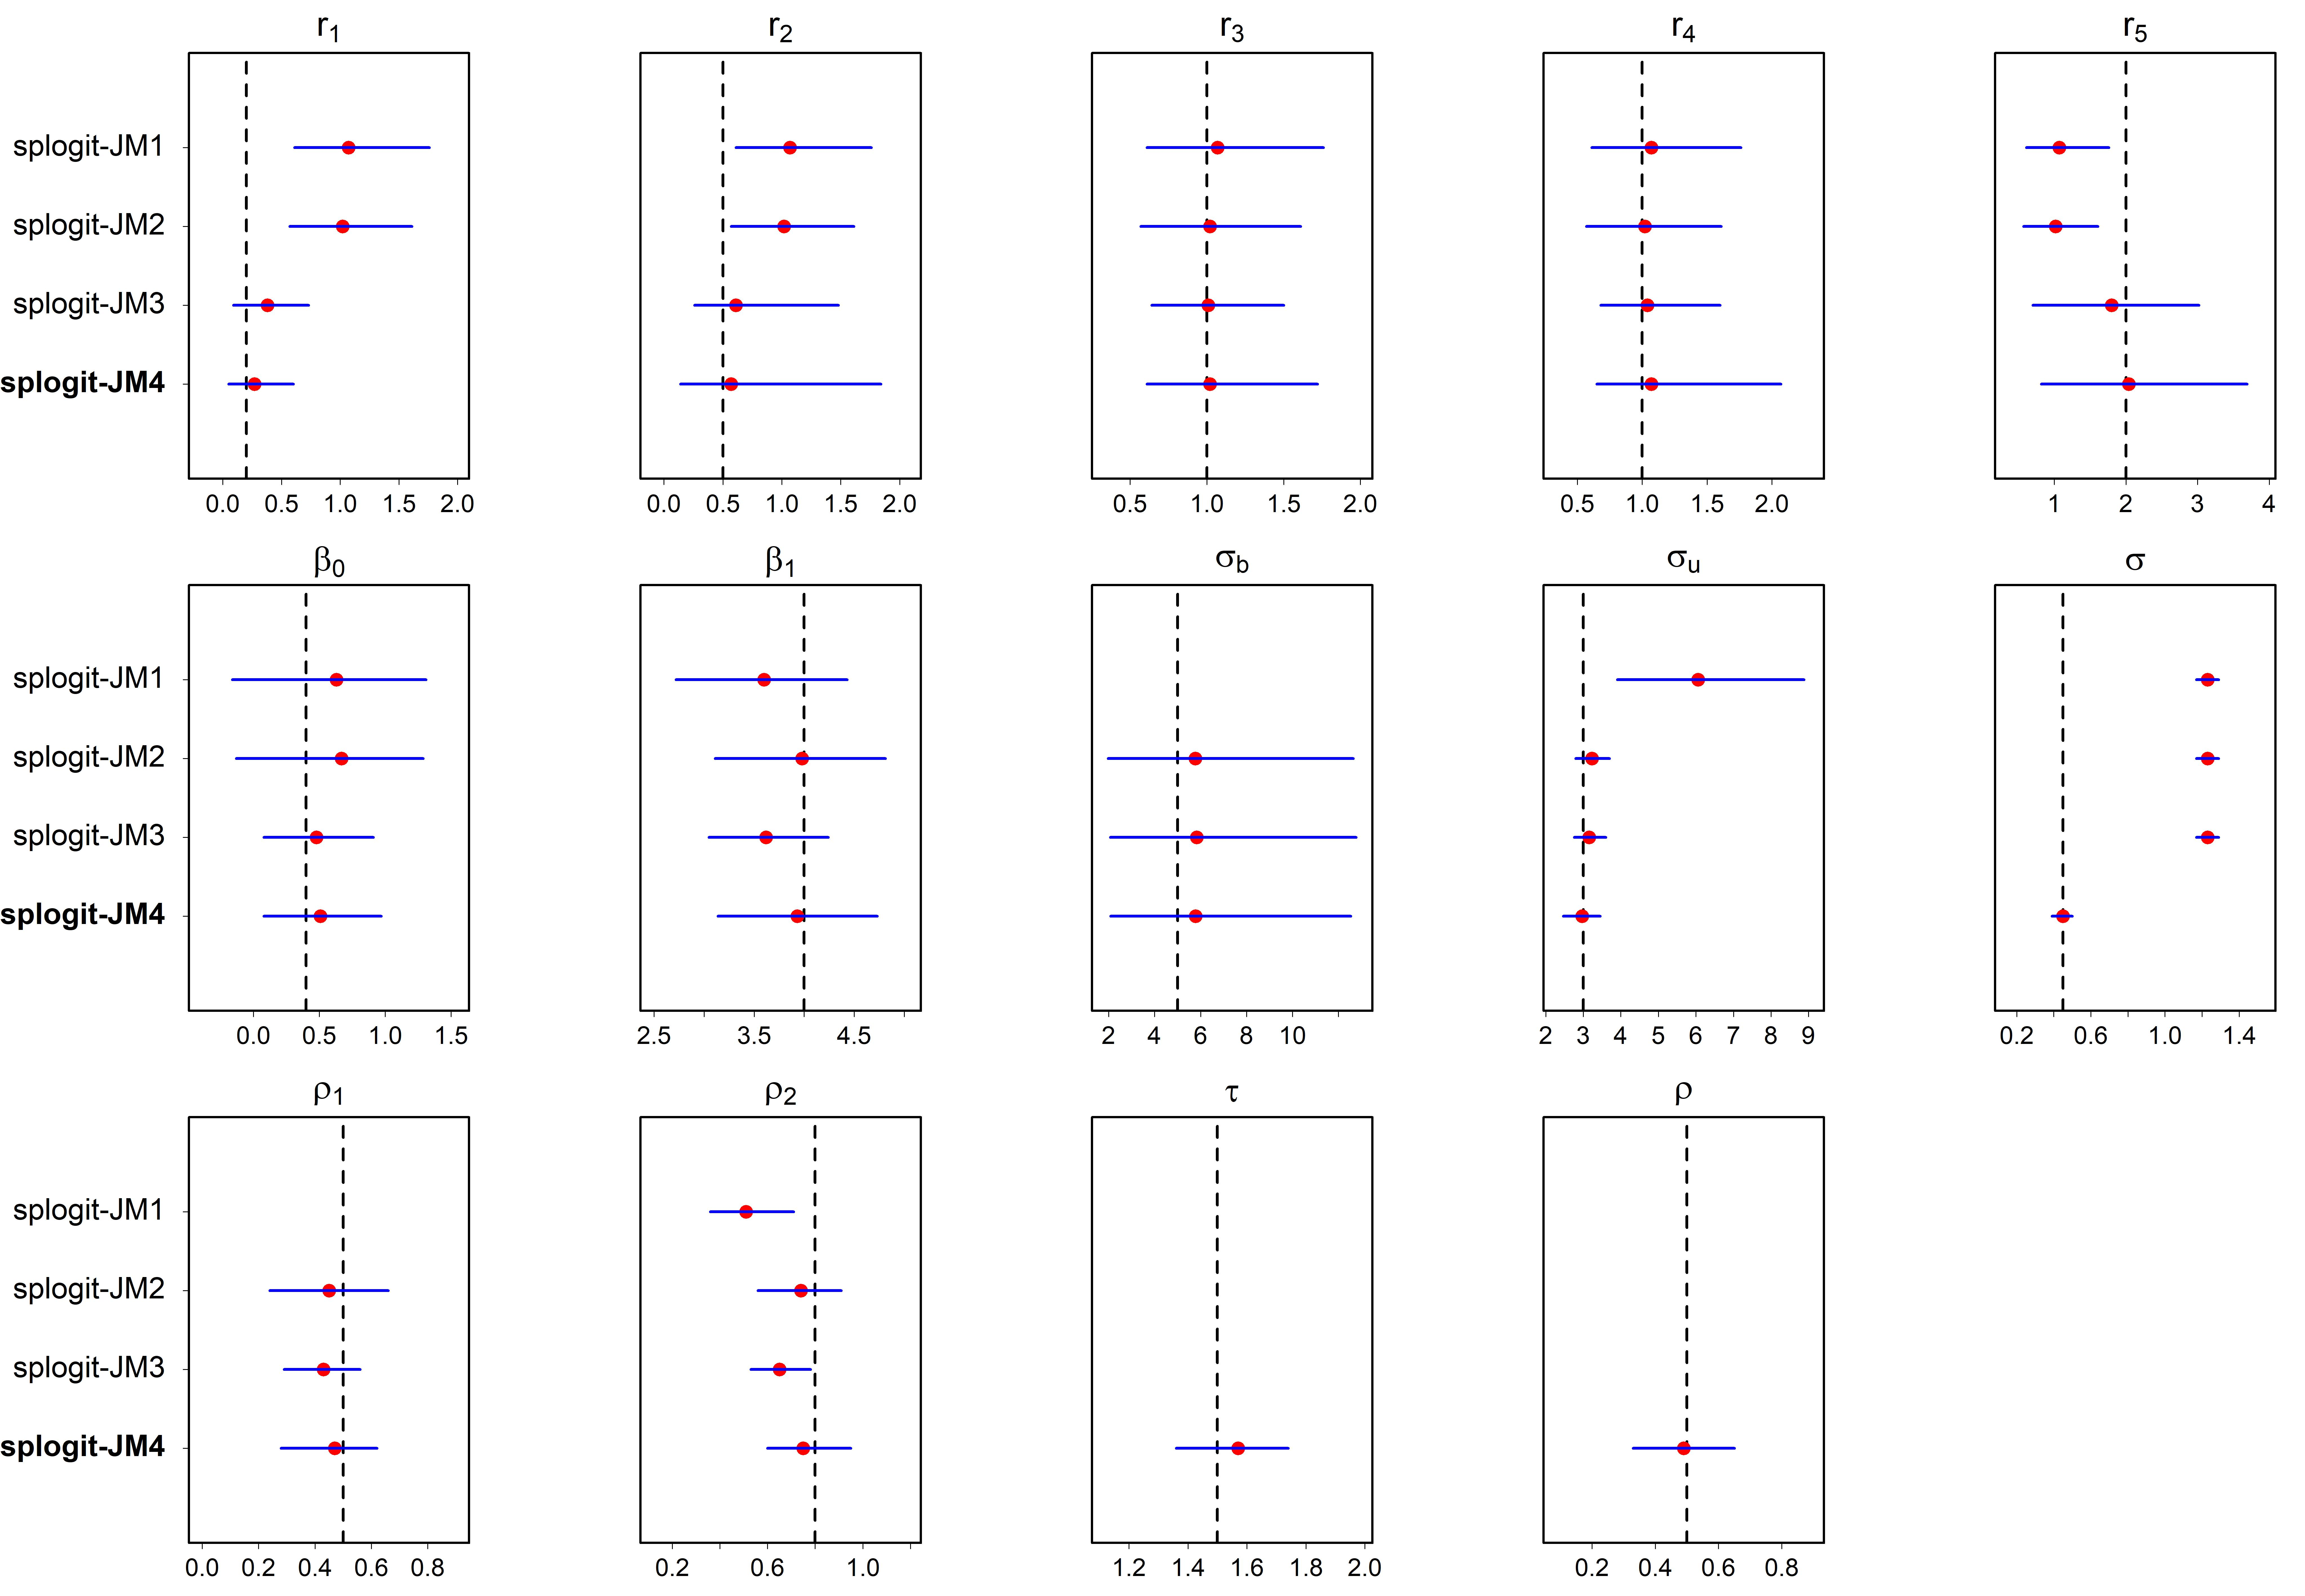
\includegraphics[width=\textwidth]{Figures/Chp2_SIM_SPLOGIT_B.jpg}
\caption{Averaged posterior means by 50 replicates via RStan with true model (boldface),  rue value (dashed vertical line), posterior mean estimates (red dot) and corresponding 95\% credible interval (blue line). JM1: Misspecified JM; JM2: No center-index JM; JM3: No covariance JM. }
\label{fig:chp2_simb1}
\end{figure}


\begin{figure}[ht]
\centering
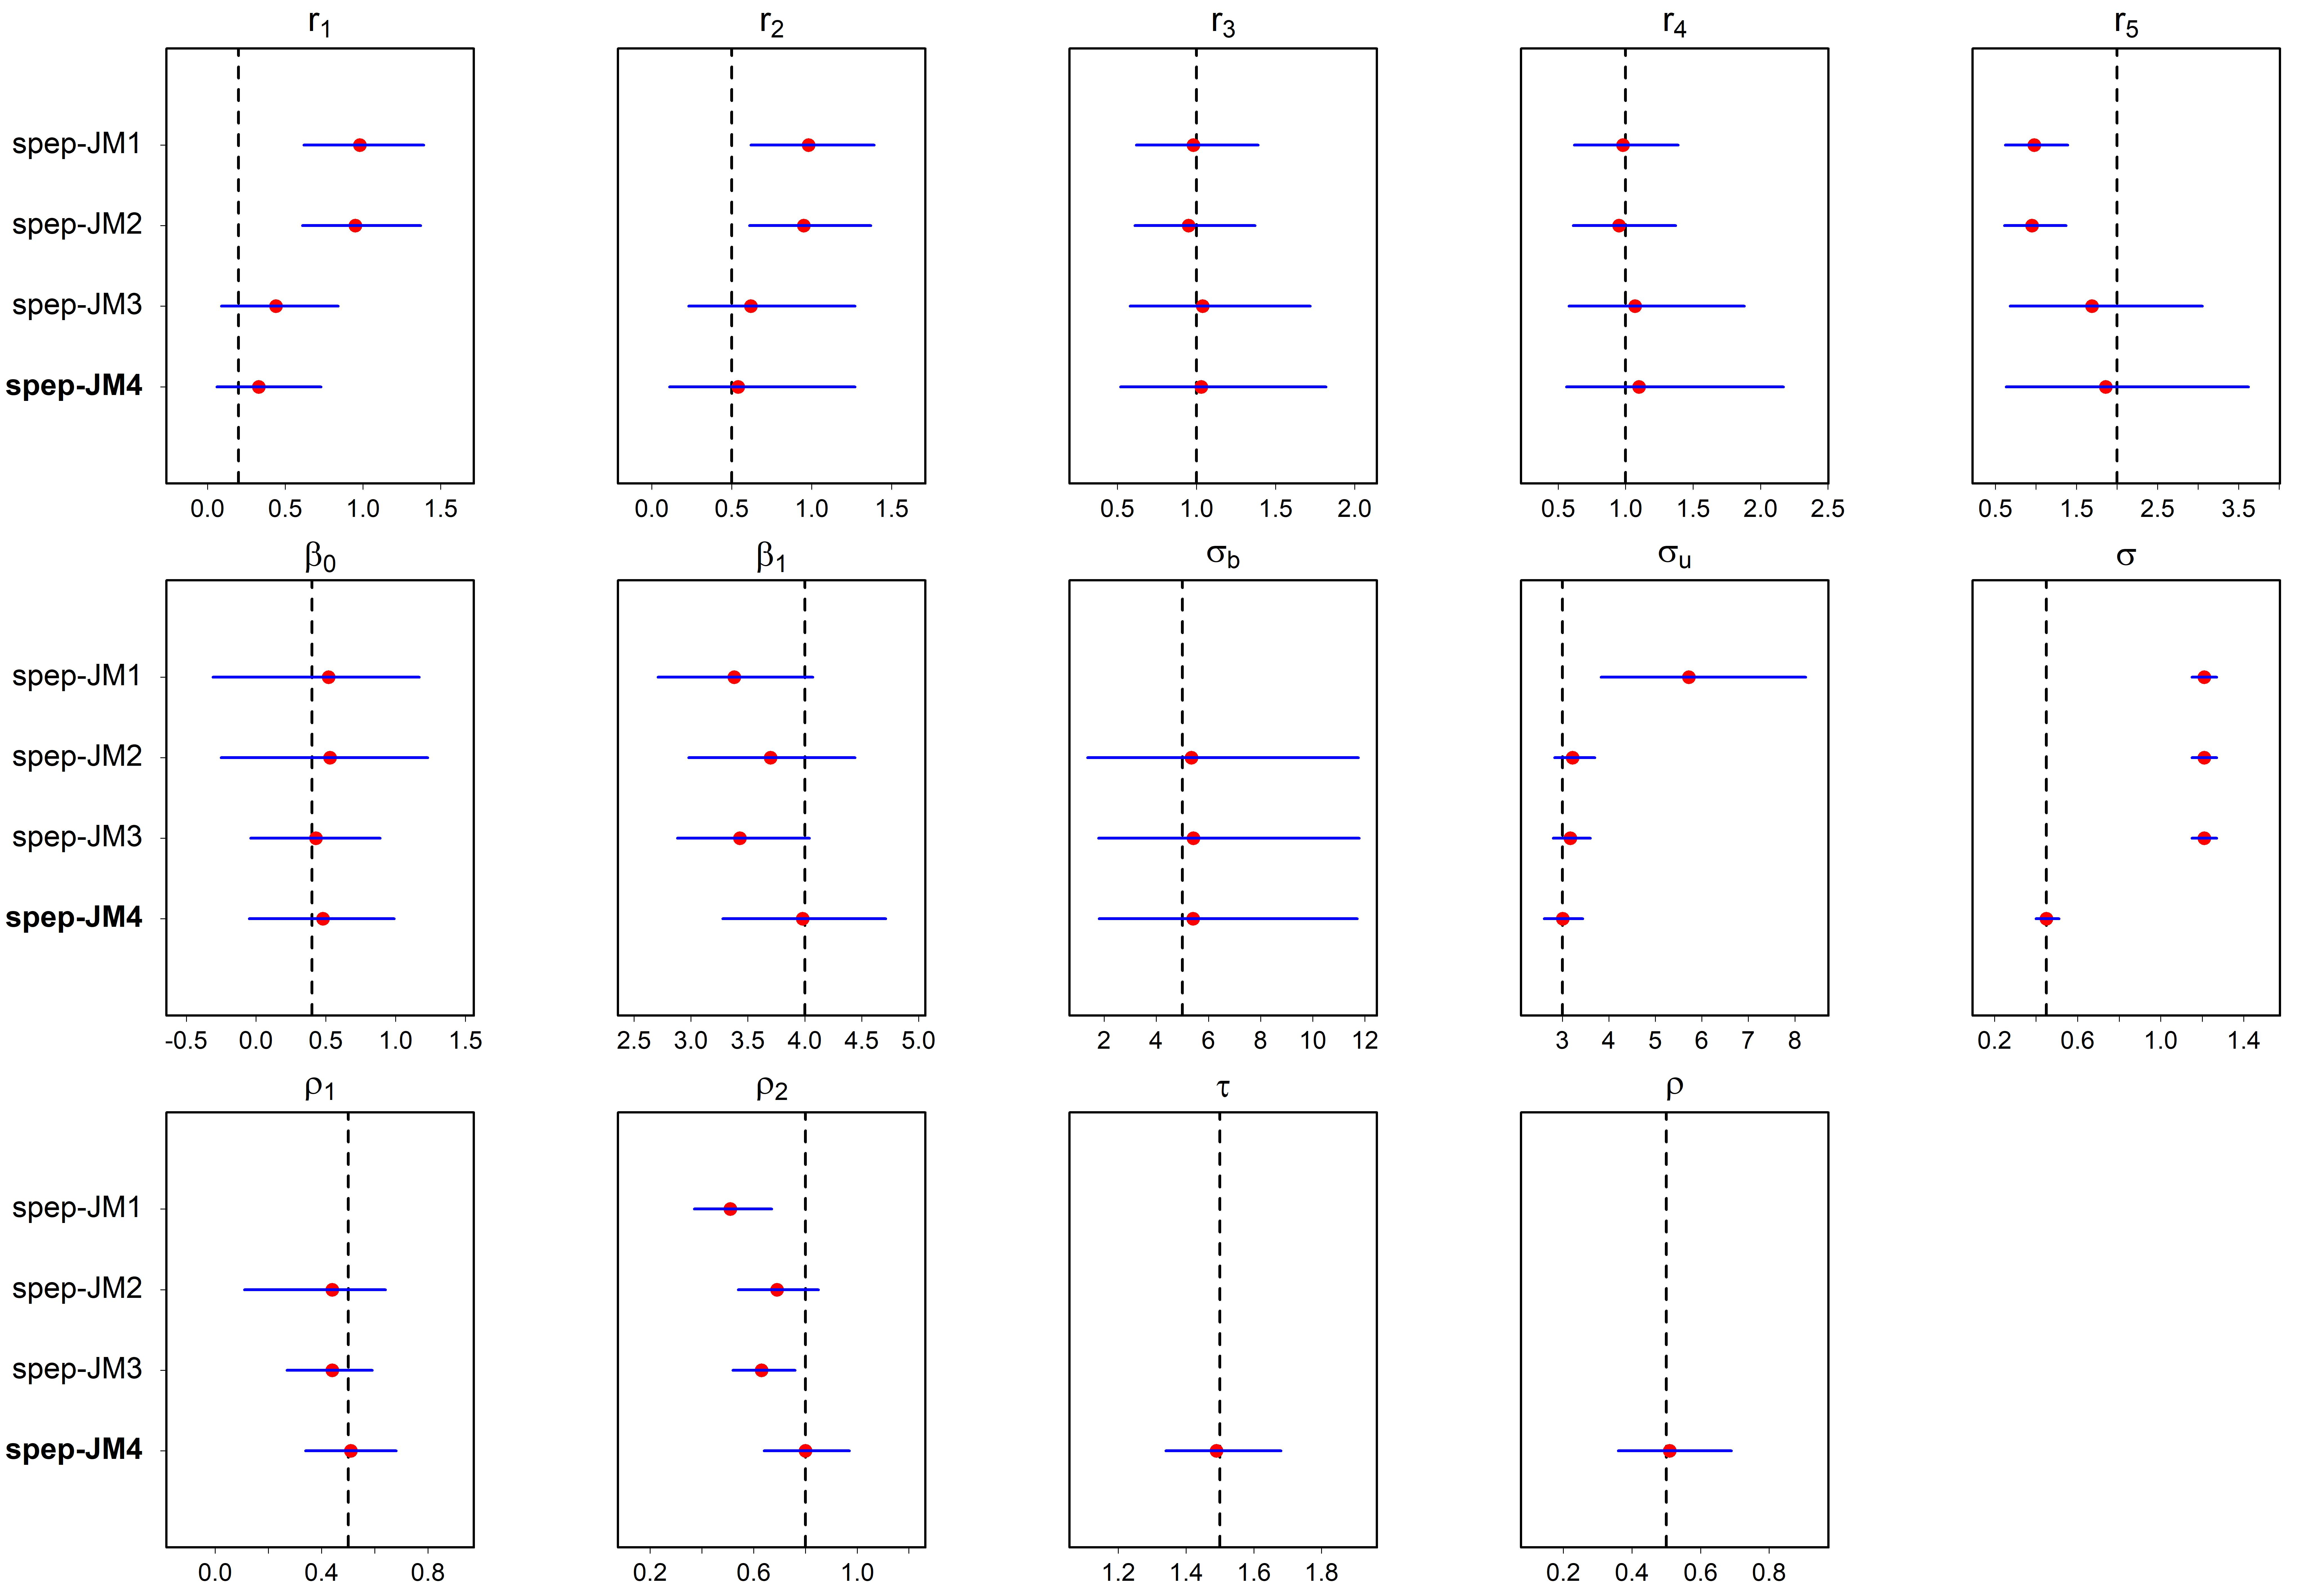
\includegraphics[width=\textwidth]{Figures/Chp2_SIM_SPEP_B.jpg}
\caption{Averaged posterior means by 50 replicates via RStan with true model (boldface),  rue value (dashed vertical line), posterior mean estimates (red dot) and corresponding 95\% credible interval (blue line). JM1: Misspecified JM; JM2: No center-index JM; JM3: No covariance JM. }
\label{fig:chp2_simb2}
\end{figure}

\section{Application} \label{sec:chp2_app}

\subsection{Motivating Data}
Our analysis cohort for this application consists of 381 CF patients who contributed a total of 9,209 observations across five centers. These centers are randomly selected among those with feasible sample size between 50 and 100 for computational aspects of the modeling. Around 15\% of measurements are excluded due to missing values on ppFEV1 and Body Mass Index (BMI). We observe neither drop-outs (e.g. death or lung transplantation) nor patients switch centers during the observed period. Data cleaning and descriptive statistics are summarized in Appendix \ref{app:b}. Approval for the data analysis was made by the Institutional Review Boards from Cincinnati Children's Hospital Medical Center and University of Cincinnati. 

\begin{figure}[ht]
\centering
\includegraphics[width=\textwidth]{Figures/Chp2_display.jpg}
\caption{Observed ppFEV1 (left panel) and density of PE (right panel) against time since the first PE occurrence. Within each longitudinal plot: three randomly selected patient profiles (solid black lines), observed values (gray dots), and center-specific LOWESS smoothing curves with 95\% confidence interval (blue solid lines with gray-shaded bands); Within each density plot: histograms (bars) with densities (areas) grouped by PE occurrence; Abbreviation: Freq. = frequency}
\label{display}
\end{figure}

We restrict encounter age to include observations taken under valid pulmonary function testing (above 6 years old) and up to early adolescence (12 years old). The upper limit is chosen to restrict the cohort to the first bout of lung function decline, which is shown to occur before more rapid decline during late adolescence and early adulthood \cite{Szczesniak2014}. To be included in the analysis, patients should have at least three or more observed ppFEV1 measurements spanning at least six months after the first PE occurrence. The time period selected for this analysis is from calendar year 2003 to 2017, because modern predictors with encounter levels are consistently documented beginning in 2003 \cite{Knapp2016}. Average (range) duration of follow-up is 4.08 (0.53-5.99) years. Figure \ref{display} displays trajectories of ppFEV1 and densities of PE throughout the whole analysis period. The left panel demonstrates the heterogeneous nature of ppFEV1 with a slightly increasing, smoothing curve in each center. The right panel indicates some underlying skewness of PE responses. 

\subsection{Internal Validation}

To access the predictive performance, we conduct 80-20\% cross-validation by choosing a random sample of 20\% of patients from each center, in which 79 patients with 1993 observations are for testing cohort. Among those remaining 80\% patients, we select the first 80\% observations with at least three records spanning at least six months after the first PE for the training cohort, which consists of 302 patients with 5769 observations and the rest of their 1447 observations are conformed as the masking cohort.

\subsection{Model Estimation}

Predictors are selected by a conventional \emph{Stepwise} method (\cite{Hocking1976}) from a two-stage model basis. We apply the R function \emph{buildlme} from \emph{buildmer} package \cite{buildmer2021} for LME submodel and the R function \emph{step} from \emph{stats} package \cite{R2020} for GLMM. By defining the baseline as the time of the first PE event, we finally include baseline ppFEV1, BMI percentile, Methicillin-resistant Staphylococcus aureus (MRSA), pseudomonas aeruginosa (pa) and genotype F508del heterozygote for the LME submodel; time since baseline (in years), BMI percentile, pancreatic enzyme usage and pa for the GLMM.

\begin{center}
\begin{table}[H]
 \caption{Model comparisons for CF data with the boldface as the preferred model.} \label{tab:chp2_app_waic}
 \centering
   \begin{threeparttable}
  \begin{tabular}{m{0.3\textwidth}m{0.15\textwidth}m{0.15\textwidth}m{0.15\textwidth}}
    \toprule
 Fitted Model & $\mbox{WAIC} \tnote{a} $ & $\mbox{WAIC}_1 \tnote{b} $ & $\mbox{WAIC}_2 \tnote{c} $ \\
 \midrule 
   Misspecified (spep-$\mbox{JM}_1$) & 49960.1 &	44302.0	& 5658.1\\
    No center-index (spep-$\mbox{JM}_2$) & 49867.6 &	44244.8	& 5622.8\\
    No covariance (spep-$\mbox{JM}_3$)  & 49812.0 & 44228.0 & 5584.0\\
   \bf Proposed (spep-$\mbox{JM}_4$) & \bf 47082.3 & \bf 42704.8 & \bf 4377.5\\
    \bottomrule
  \end{tabular}
   \begin{tablenotes}[para]
    \footnotesize
        \item[a] Joint model; \item[b] Continuous submodel; \item[c] Binary submodel
    \end{tablenotes}
     \end{threeparttable}
\end {table}
\end{center}

Given flexible spep link is superior to splogit shown in the previous simulation Table \ref{tab:chp2_sim}, thus we examine a total of four joint models: spep-$\mbox{JM}_1$ $\sim$ spep-$\mbox{JM}_4$ for the training cohort. Posterior samplings are carried out by HMC with 2000 post-warmup draws via two chains and diagnostics plots (see Appendix \ref{app:b} for details) show that all samplings are well converged. Model performance with respect to WAIC is presented in Table \ref{tab:chp2_app_waic}, undoubtedly model spep-$\mbox{JM}_4$ outperforms others with the lowest WAIC. spep-$\mbox{JM}_1$ yields the worst WAIC which demonstrates underlying biases caused by a non-hierarchical model in the CF study. To further evaluate the assumption of longitudinal submodel in spep-$\mbox{JM}_4$, we have plotted residual diagnostics in Appendix \ref{app:b}. No striking violations are found by the visual inspections. 

\begin{center}
\begin{table}[ht]
   \caption{Model estimations under spep-$\mbox{JM}_4$} \label{tab:chp2_est}
   \centering
    \begin{threeparttable}
  \begin{tabular}{lcccccccc}
    \toprule
  & mean \tnote{1} & se \tnote{2} & sd \tnote{3} & 2.5\% \tnote{4} & 97.5\% \tnote{4} & n\_eff \tnote{5} & Rhat \tnote{6}\\
 \midrule
   \textbf{Continuous submodel} &&&&&&& \\
   \midrule
    $\alpha_1$ (intercept at age 6 years) & 27.64&0.07&2.50&22.68&32.75&1333.36&1.00\\
    $\alpha_2$ (BMI percentile) & 0.20&0.00&0.01&0.18&0.22&1959.51&1.00\\
    $\alpha_3$ (ppFEV1 at baseline) & 0.56&0.00&0.03&0.51&0.61&1272.50&1.00\\
    $\alpha_4$ (MRSA) & -1.02&0.01&0.50&-1.99&-0.06&2265.35&1.00\\
    $\alpha_5$ (pa) & -0.54&0.01&0.42&-1.38&0.27&2191.20&	1.00\\
    $\alpha_6$ (F508del Heterozygote) & 2.47&0.03&1.23&-0.04&4.83&1284.23&1.00\\
    $\sigma_b$ (between centers, intercept) & 1.49&0.05&1.26&0.07&4.51&702.15&1.00\\
    $\sigma_u$ (between patients, intercept) & 3.38&0.02&0.66&2.12&4.70&716.09&1.00 \\
    $\sigma$ (measurement error) & 8.77&0.00&0.11&8.55&8.98&1563.44&1.00\\
    $\tau$ (scale parameter) & 11.20&0.01&0.36&10.53&11.93&1463.20&1.00\\
    $\rho$ (1/range)& 0.41&0.00&0.04&0.34&0.50&1213.08&1.00\\
  \midrule
  \textbf{Binary submodel} &&&&&&& \\
   \midrule
    $\beta_1$ (intercept at age 6 years) & 2.94&0.01&0.23&2.53&3.40&1375.26&1.00\\
    $\beta_2$ (time) & -0.37&0.00&0.02&-0.42&-0.33&1920.79&1.00\\
    $\beta_3$ (BMI percentile) & -0.01&0.00&0.00&-0.01&-0.01&1535.26&1.00\\
    $\beta_4$ (Enzymes) & -0.13&0.00&0.06&-0.25&-0.03&1811.64&1.00\\
    $\beta_5$ (pa) & -0.22&0.00&0.07&-0.35&-0.09&2030.46&1.00\\
    $r_1$ (power parameter, Center 1) &3.99	&0.03&1.41&1.94&7.42&1887.80&1.00\\
    $r_2$ (power parameter, Center 2) & 2.76&0.03&1.24&1.27&6.15&1509.01&1.00\\
    $r_3$ (power parameter, Center 3)& 2.76&0.03&1.12&1.29&5.62&1672.64&1.00\\
    $r_4$ (power parameter, Center 4)& 4.23&0.04&1.60&1.86&7.90&1480.30&1.00\\
    $r_5$ (power parameter, Center 5)& 2.93&0.03&1.21&1.40&6.09&1831.08&1.00\\
  \midrule
 \textbf{Association} &&&&&&& \\
  \midrule
    $\rho_1$ (submodel link, center) & -0.20&0.01&0.30&-0.81&0.63&402.58&1.01\\
    $\rho_2$ (submodel link, patient) & -0.44&0.00&0.10&-0.68&-0.30&606.82&1.00\\
    \bottomrule
  \end{tabular}
 \begin{tablenotes}[para]
    \footnotesize
    \item[1] posterior mean; \item[2] Monte Carlo standard error; \item[3] Monte Carlo standard deviation; \item[4] posterior quantiles; \item[5] effective sample size; \item[6] potential scale reduction factor (at convergence, Rhat=1)
    \end{tablenotes}
    \end{threeparttable}
\end {table}
\end{center}

The estimations for spep-$\mbox{JM}_4$ are summarized in Table \ref{tab:chp2_est}. For continuous submodel, baseline ppFEV1 and BMI percentile imply significantly positive relationship with ppFEV1. In Taylor-Robinson's study \cite{TaylorRobinson2012}, they found that people with high ppFEV1 at baseline were more likely to have a higher ppFEV1 up to 15 years, which reconciles the positive effect of baseline ppFEV1 as in ours. Categorical predictors MRSA and pa correspond to worsen overall ppFEV1, though pa is not significant because 95\% credible interval contains zero. Significant parameter $\rho$ indicates that the correlation between two measurements within a patient decays as time elapses. For binary submodel, the risk of PE onset is decreasing against time given all the other predictors unchanged. BMI percentile plays an important role in ppFEV1, however, it seems not to contribute much for PE. The infection with pa and pancreatic enzyme usage are associated with lower PE frequency. The interpretations would be most likely that patients who are infected by pa or with insufficient pancreatic enzyme are given primary medical care. Negative association parameter $\rho_1$ significantly suggests that the center with more severe CF patients (indicated by the lower $b_l$) tends to have higher risk of PE; Analogously, negative $\rho_2$ significantly indicates that patients with worse averaged lung function (indicated by the lower $U_{li}$) are more likely to experience PE.

\subsection{Predictive Performance}

We utilize root mean squared error (RMSE) and area under curve (AUC) to evaluate continuous and binary predictions, respectively. AUC is a measurement for the classification, thus the higher AUC, the better the model is at distinguishing between PE and non-PE events. Corresponding results along with residuals standard error and 95\% confidence intervals are summarized in Table \ref{tab:chp2_pd} and \ref{tab:chp2_fc}.
 
\begin{table}[ht]
 \caption{Predictive performance between training and testing cohorts} \label{tab:chp2_pd}
  \centering
  \resizebox{\columnwidth}{!}{%
   \begin{threeparttable}
  \begin{tabular}{lrcccrccc}
    \toprule
  & \multicolumn{4}{c} {Training} &  \multicolumn{4}{c} {Testing}\\
    \cmidrule(lr) {2-5} \cmidrule(lr) {6-9}
     & \multicolumn{2}{c} {ppFEV1} &  \multicolumn{2}{c} {PE} & \multicolumn{2}{c} {ppFEV1} &  \multicolumn{2}{c} {PE}\\
    \cmidrule(lr) {2-3} \cmidrule(lr) {4-5} \cmidrule(lr) {6-7} \cmidrule(lr) {8-9}
 {spep-JM} & RMSE & SE & AUC & 95\% CIs & RMSE & SE & AUC & 95\% CIs \\
 \midrule
   
   {Misspecified ($\mbox{JM}_1$)}
  & 10.755 & 0.142 & 0.748 & (0.734, 0.763) & 10.397 & 0.233 & 0.623 & (0.594, 0.651)\\

   {No center-index ($\mbox{JM}_2$)}
  & 10.686 & 0.141 & 0.748 & (0.734, 0.763)	& 10.399 & 0.233 & 0.622 & (0.593, 0.651)\\

   {No covariance ($\mbox{JM}_3$)}
  & 10.671 & 0.141 & 0.755 & (0.741, 0.770) & 10.398 & 0.233 & 0.639 & (0.610, 0.667)\\
   {Proposed ($\mbox{JM}_4$)}
   & 7.768	& 0.102 & 0.882 & (0.873, 0.892) & 6.879 & 0.154 & 0.631 & (0.604, 0.658)\\
    \bottomrule
  \end{tabular}
   \begin{tablenotes}[para]
    \footnotesize
     Abbreviations: RMSE=Root Mean Square Error; SE=Standard Error; AUC=Area under Curve; CI=Confidence Interval 
    \end{tablenotes}
    \end{threeparttable}%
}
 \end {table}

\begin{table}[ht]
\caption{Forecasting performance between training and masking cohorts} \label{tab:chp2_fc}
\centering
\resizebox{\columnwidth}{!}{%
 \begin{threeparttable}
  \begin{tabular}{lrcccrccc}
    \toprule
  & \multicolumn{4}{c} {Training} &  \multicolumn{4}{c} {Masking}\\
    \cmidrule(lr) {2-5} \cmidrule(lr) {6-9}
     & \multicolumn{2}{c} {ppFEV1} &  \multicolumn{2}{c} {PE} & \multicolumn{2}{c} {ppFEV1} &  \multicolumn{2}{c} {PE}\\
    \cmidrule(lr) {2-3} \cmidrule(lr) {4-5} \cmidrule(lr) {6-7} \cmidrule(lr) {8-9}
 {spep-JM} & RMSE & SE & AUC & 95\% CIs & RMSE & SE & AUC & 95\% CIs \\
 \midrule
   
   {Misspecified ($\mbox{JM}_1$)}
  & 10.755 & 0.142 & 0.748 & (0.734, 0.763) & 10.354 & 0.272 & 0.655 & (0.626, 0.683) \\

   {No center-index ($\mbox{JM}_2$)}
  & 10.686 & 0.141 & 0.748 & (0.734, 0.763)	& 10.298 & 0.270 & 0.628 & (0.598, 0.658)\\

   {No covariance ($\mbox{JM}_3$)}
  & 10.671 & 0.141 & 0.755 & (0.741, 0.770) & 10.353 & 0.271 & 0.612 & (0.582, 0.642)\\
   {Proposed ($\mbox{JM}_4$)}
   & 7.768	& 0.102 & 0.882 & (0.873, 0.892) & 8.850 & 0.233 & 0.785 & (0.760, 0.809)\\
    \bottomrule
  \end{tabular}
    \begin{tablenotes}[para]
    \footnotesize
     Abbreviations: RMSE=Root Mean Square Error; SE=Standard Error; AUC=Area under Curve; CI=Confidence Interval 
    \end{tablenotes}
    \end{threeparttable}%
}
 \end {table}

\begin{figure}[ht]
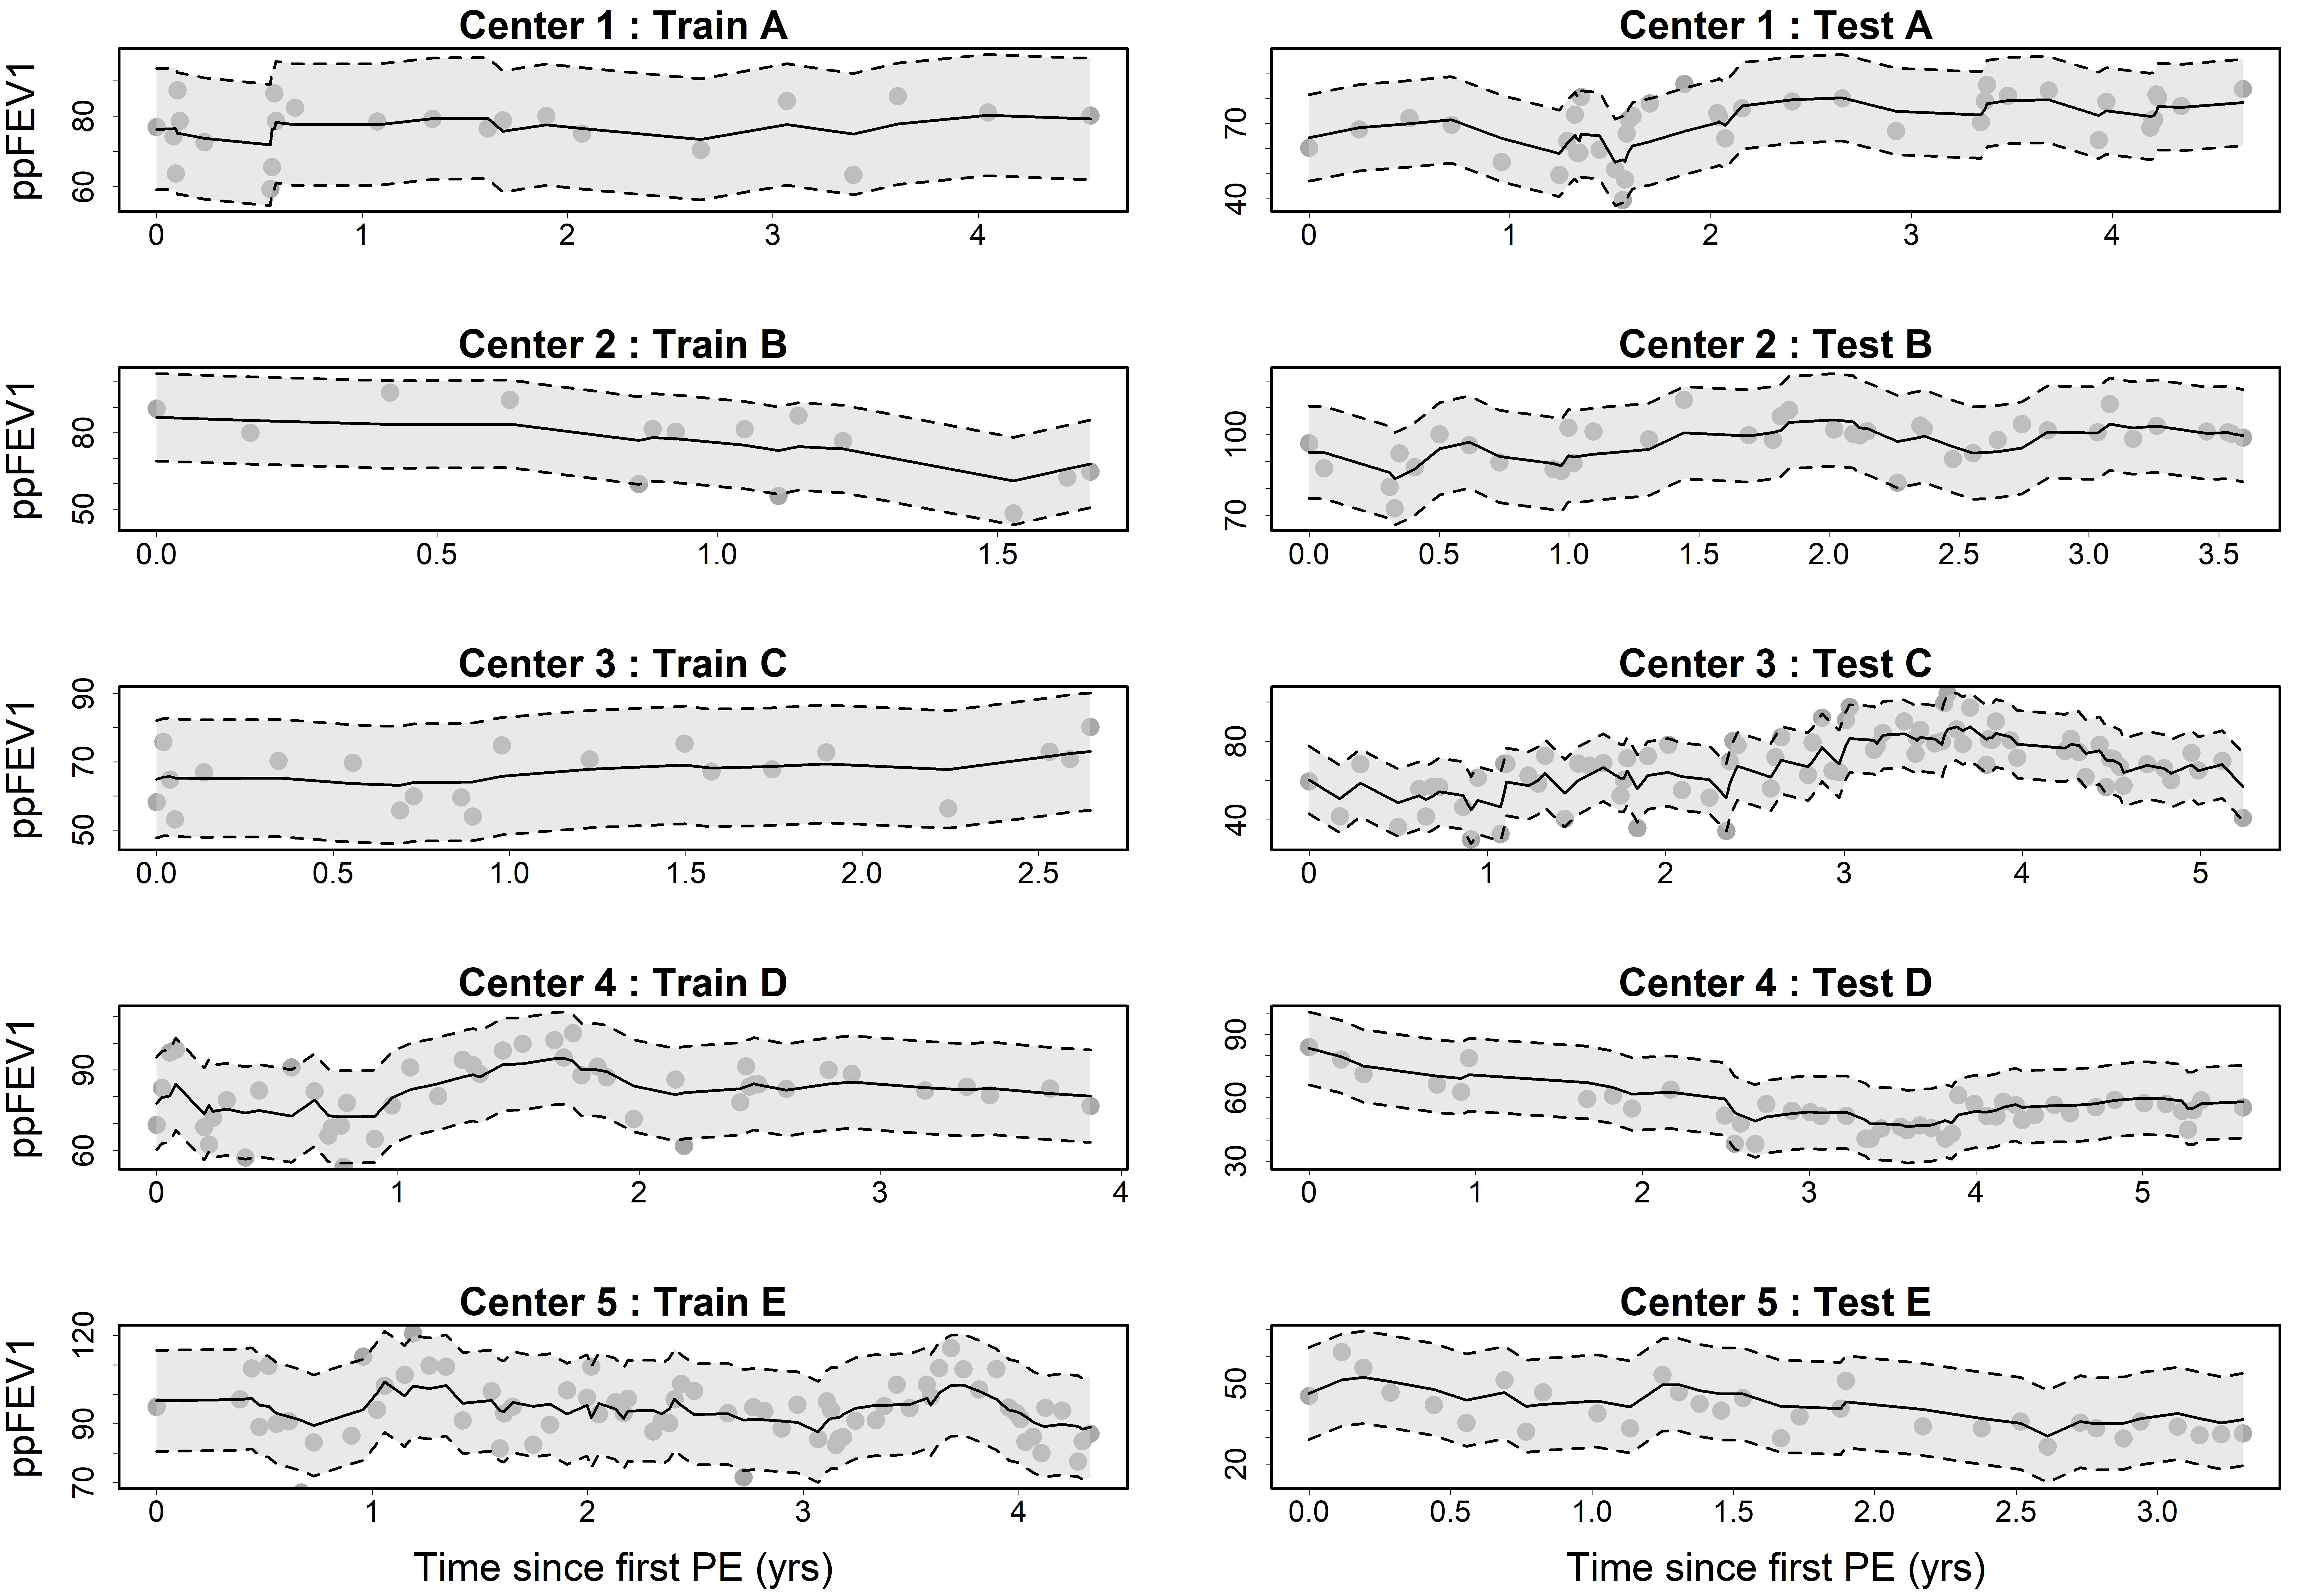
\includegraphics[width=\textwidth]{Figures/Chp2_pred.jpg}
\caption{Prediction for random selected patients from each center under spep-$\mbox{JM}_4$ model, including observed ppFEV1 (gray dots) against time with fitted values (solid lines) and corresponding 95\% CIs (bands)}
\label{fig:pred}
\end{figure}

\begin{figure}[ht]
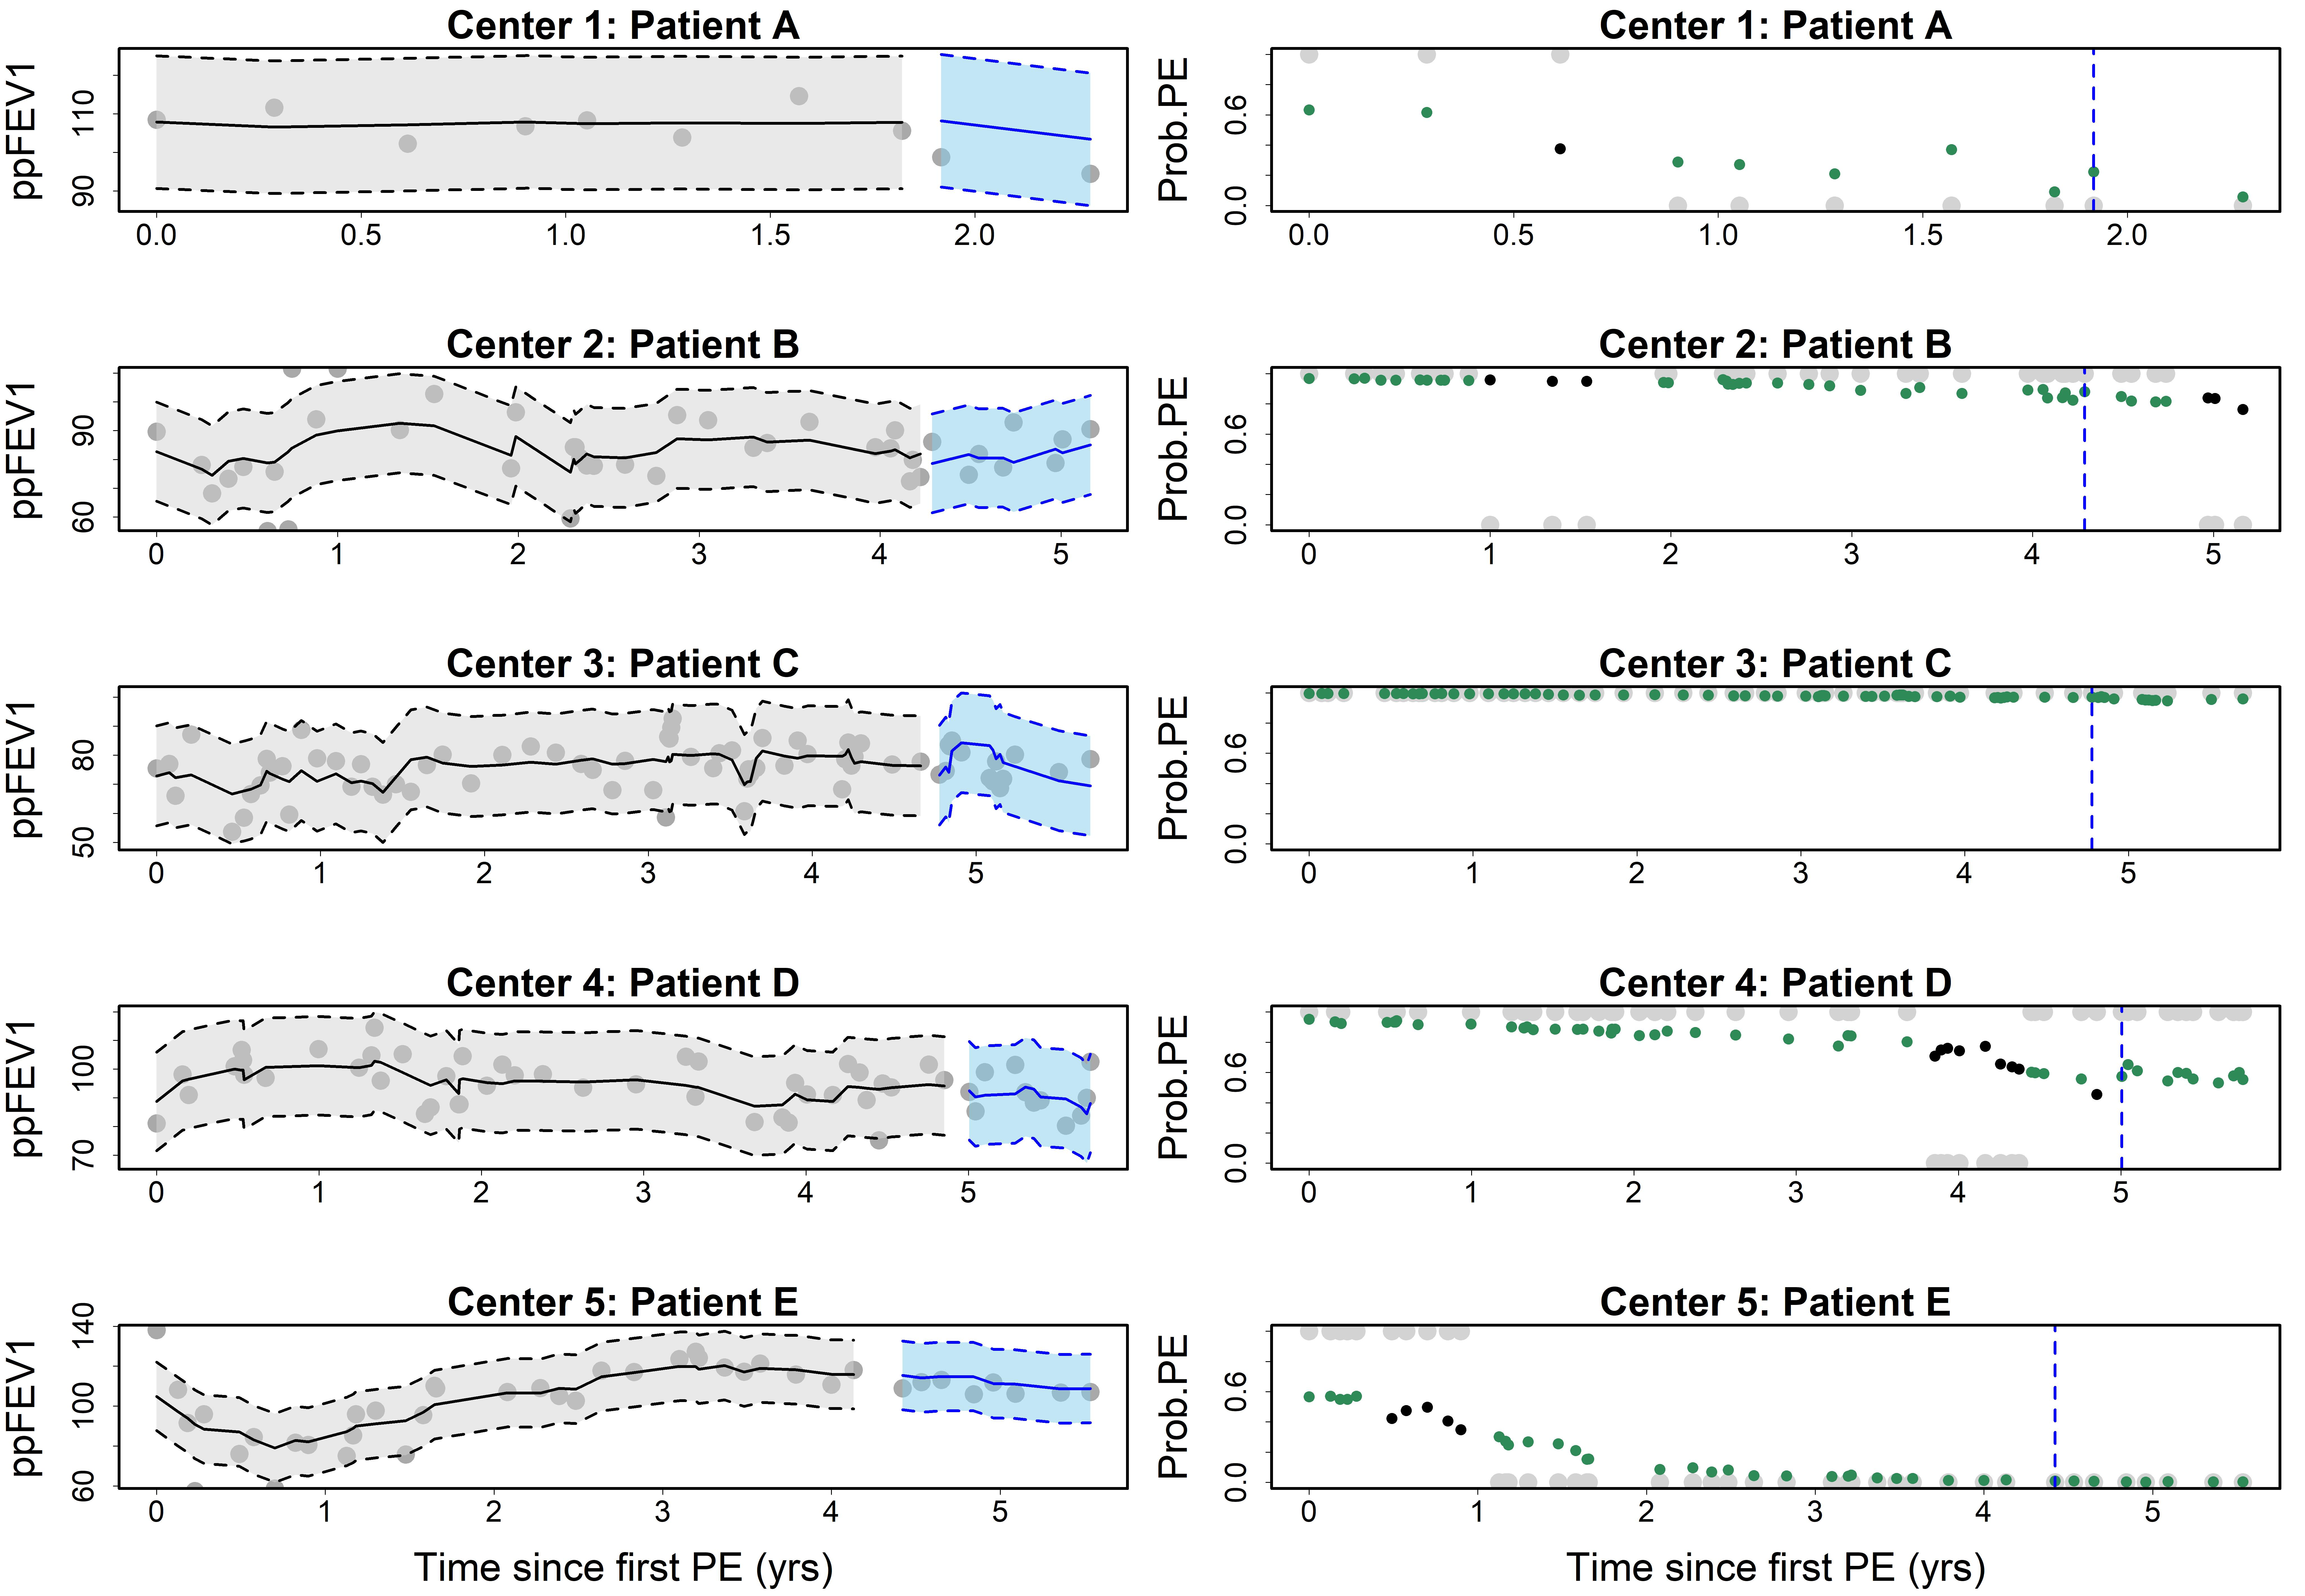
\includegraphics[width=\textwidth]{Figures/Chp2_mask.jpg}
\caption{Forecast for random selected patients from each center under spep-$\mbox{JM}_4$ model, including observed ppFEV1 (gray dots) against time with fitted (solid black lines) and prognostic values (solid blue lines) and corresponding 95\% CIs (bands); observed PE (gray dots) against time with predicted probability of PE onset (green dots for the true classification; black dots for the false classification)}
\label{fig:fcast}
\end{figure}

Table \ref{tab:chp2_pd} shows that spep-$\mbox{JM}_4$ achieves the smallest RMSE and the highest AUC for the training cohort. We note that the difference in accuracy is not evident from spep-$\mbox{JM}_1$ to spep-$\mbox{JM}_4$ for the testing cohort, however, the smallest RMSE is convincing enough to conclude spep-$\mbox{JM}_4$ as the optimal choice. We apply the same training cohort to examine the forecasting performance of each model. Table \ref{tab:chp2_fc} also demonstrates that spep-$\mbox{JM}_4$ is outstanding in forecasting performance. Figure \ref{fig:pred} and \ref{fig:fcast} present individual prediction and forecast under spep-$\mbox{JM}_4$ structure, respectively. Our proposed model is well shown to capture the heterogeneous nature of ppFEV1, whilst provided reasonable predictive probabilities of PE encounters.

\section{Discussion} \label{sec:chp2_con}

In this chapter, we have developed a multilevel Bayesian joint model with a flexible link function to accommodate analysis of longitudinal and binary outcomes for a monitoring CF registry data, which is depicted by hierarchical structures and irregularly observed time points. Our novel approach relaxes the inference on regular clinical follow-up from a previous study \cite{Su2020}, \cite{Su2021}, which avoids unnecessary biases caused by annualized covariates. The rationale for dynamic individual prediction is obtained by plugging posterior means from HMC method into BLUP equations as shown in Section \ref{sec:chp2_pred}. The interplay of Bayesian and frequentist approach is beneficial to both numerical and analytic analysis, especially in modern hierarchical models (\cite{Bayarri2004}). Both the simulation study and motivating example demonstrate the reliable capability of our proposed joint model. Furthermore, our model can be applied to numerous alternative hierarchical data structures, see Section 2 from Brilleman et al. \cite{Brilleman2019} for more data examples. 

For the class of flexible symmetric power link functions, our assessments favor spep over splogit from the model information criterion. In addition, the virtual distinguishes between such two links are presented in Figure \ref{fig:Chp2_cdf_sp}. The authors of the seminal flexible link function (\cite{Jiang2013}) demonstrated that, Equation \ref{eq:ch2_Fsp} achieved left skewness when $0<r<1$; symmetric when $r=1$; right skewness when $r>1$. Researchers need to be aware that this statement cannot hold when values of covariate $x$ are asymmetric (see the simulation study in Appendix \ref{app:b} for details). As a conclusion, we recommend a flexible link function regardless of whether there exists observed skewness of responses in the real data case. 

There may be some possible limitations in this study. We have focused our study on symmetric power link family only, however, an alternative is subject to a class of link functions based on the GEV distribution (\cite{Wang2010}). To the best of our knowledge, there are no existing R packages that incorporate any aforementioned flexible link families, which might be an interesting field to explore in the future research. In addition, given the fact that PE onset would be dependent on various intrinsic factors and CF is a multi-system disease, the aforementioned time-independent association structure can be further extended. Moreover, a joint model of longitudinal and time-to-recurrent outcomes is actively under the investigation with the aim to facilitate the detection of PE.


\chapter{Multilevel Bayesian joint model of longitudinal and recurrent outcomes}\label{chp3}

In previous chapter, we propose a multilevel joint model that accommodates longitudinal and binary outcomes. It also might be of clinical interest to monitor and predict the probability of next PE by regarding repeated PE in the survival context. In this chapter, we illustrate our proposed multilevel Bayesian joint model that encompasses the LME for longitudinal outcomes and the stratified relative risk frailty model for time-to-recurrent events.  

This chapter is organized as follows. In Section \ref{sec:chp3_mov}, we emphasize the motivation. In Section \ref{sec:chp3_mod}, we introduce the methodology, including framework of submodels, Bayesian inference, predictive metrics and model selection. In Section \ref{sec:chp3_sim} and \ref{sec:chp3_app}, we illustrate a simulation study and motivating example, respectively. Lastly, we conclude our study with remarks and discussions in Section \ref{sec:chp3_diss}. 

\section{Motivation} \label{sec:chp3_mov}

 In a comprehensive review paper, \cite{Hickey2018} summarized corresponding literature for joint models involving multivariate event time data, of which one stream was for recurrent events. To the best of our knowledge, numerous authors have studied jointly modeling longitudinal outcomes and recurrent events (either in the presence of a terminal event, or not), but not for hierarchical data structure (\cite{Liu2008}, \cite{Kim2012}, \cite{Musoro2015}, \cite{Shen2016}, \cite{Ren2021}) or vice versa (\cite{Luo2014}, \cite{Brilleman2019}). To this end, we are motivated to postulate a shared parameter joint model consisting of two submodels, the linear mixed effect (LME) submodel for the longitudinal trajectory and extended stratified relative risk frailty model (\cite{Rizopoulos2012b}) for the recurrent event submodel. In addition, the two submodels are linked by a center-specific latent trajectory. It is worth noting that the growing framework of latent class joint model can be employed for heterogeneous population (\cite{Han2007}, \cite{Brombin2016}). However, such model assumes that the subpopulations are latent, or in other words that heterogeneity is not capture by any of the observed covariates. Consequently, the latent class joint model might not be suitable to our study due to known center information. The visualization of our data structure along with two types of time scales to the repeated events are displayed in Figure \ref{fig:chp3_censor}. Calendar time and gap time are of the same interval time length, however, interpretations for risk predictions are different. With gap time, predictions are made for the next event at the time of the current event, while with calendar time, predictions are made for a primary event time at the entry time (\cite{Smedinga2017}). In other words, calendar time evaluates the effect of a covariate since the study entry point, while gap time evaluates the effect since the end time of the previous event. 
 
\begin{figure}[ht]
\centering
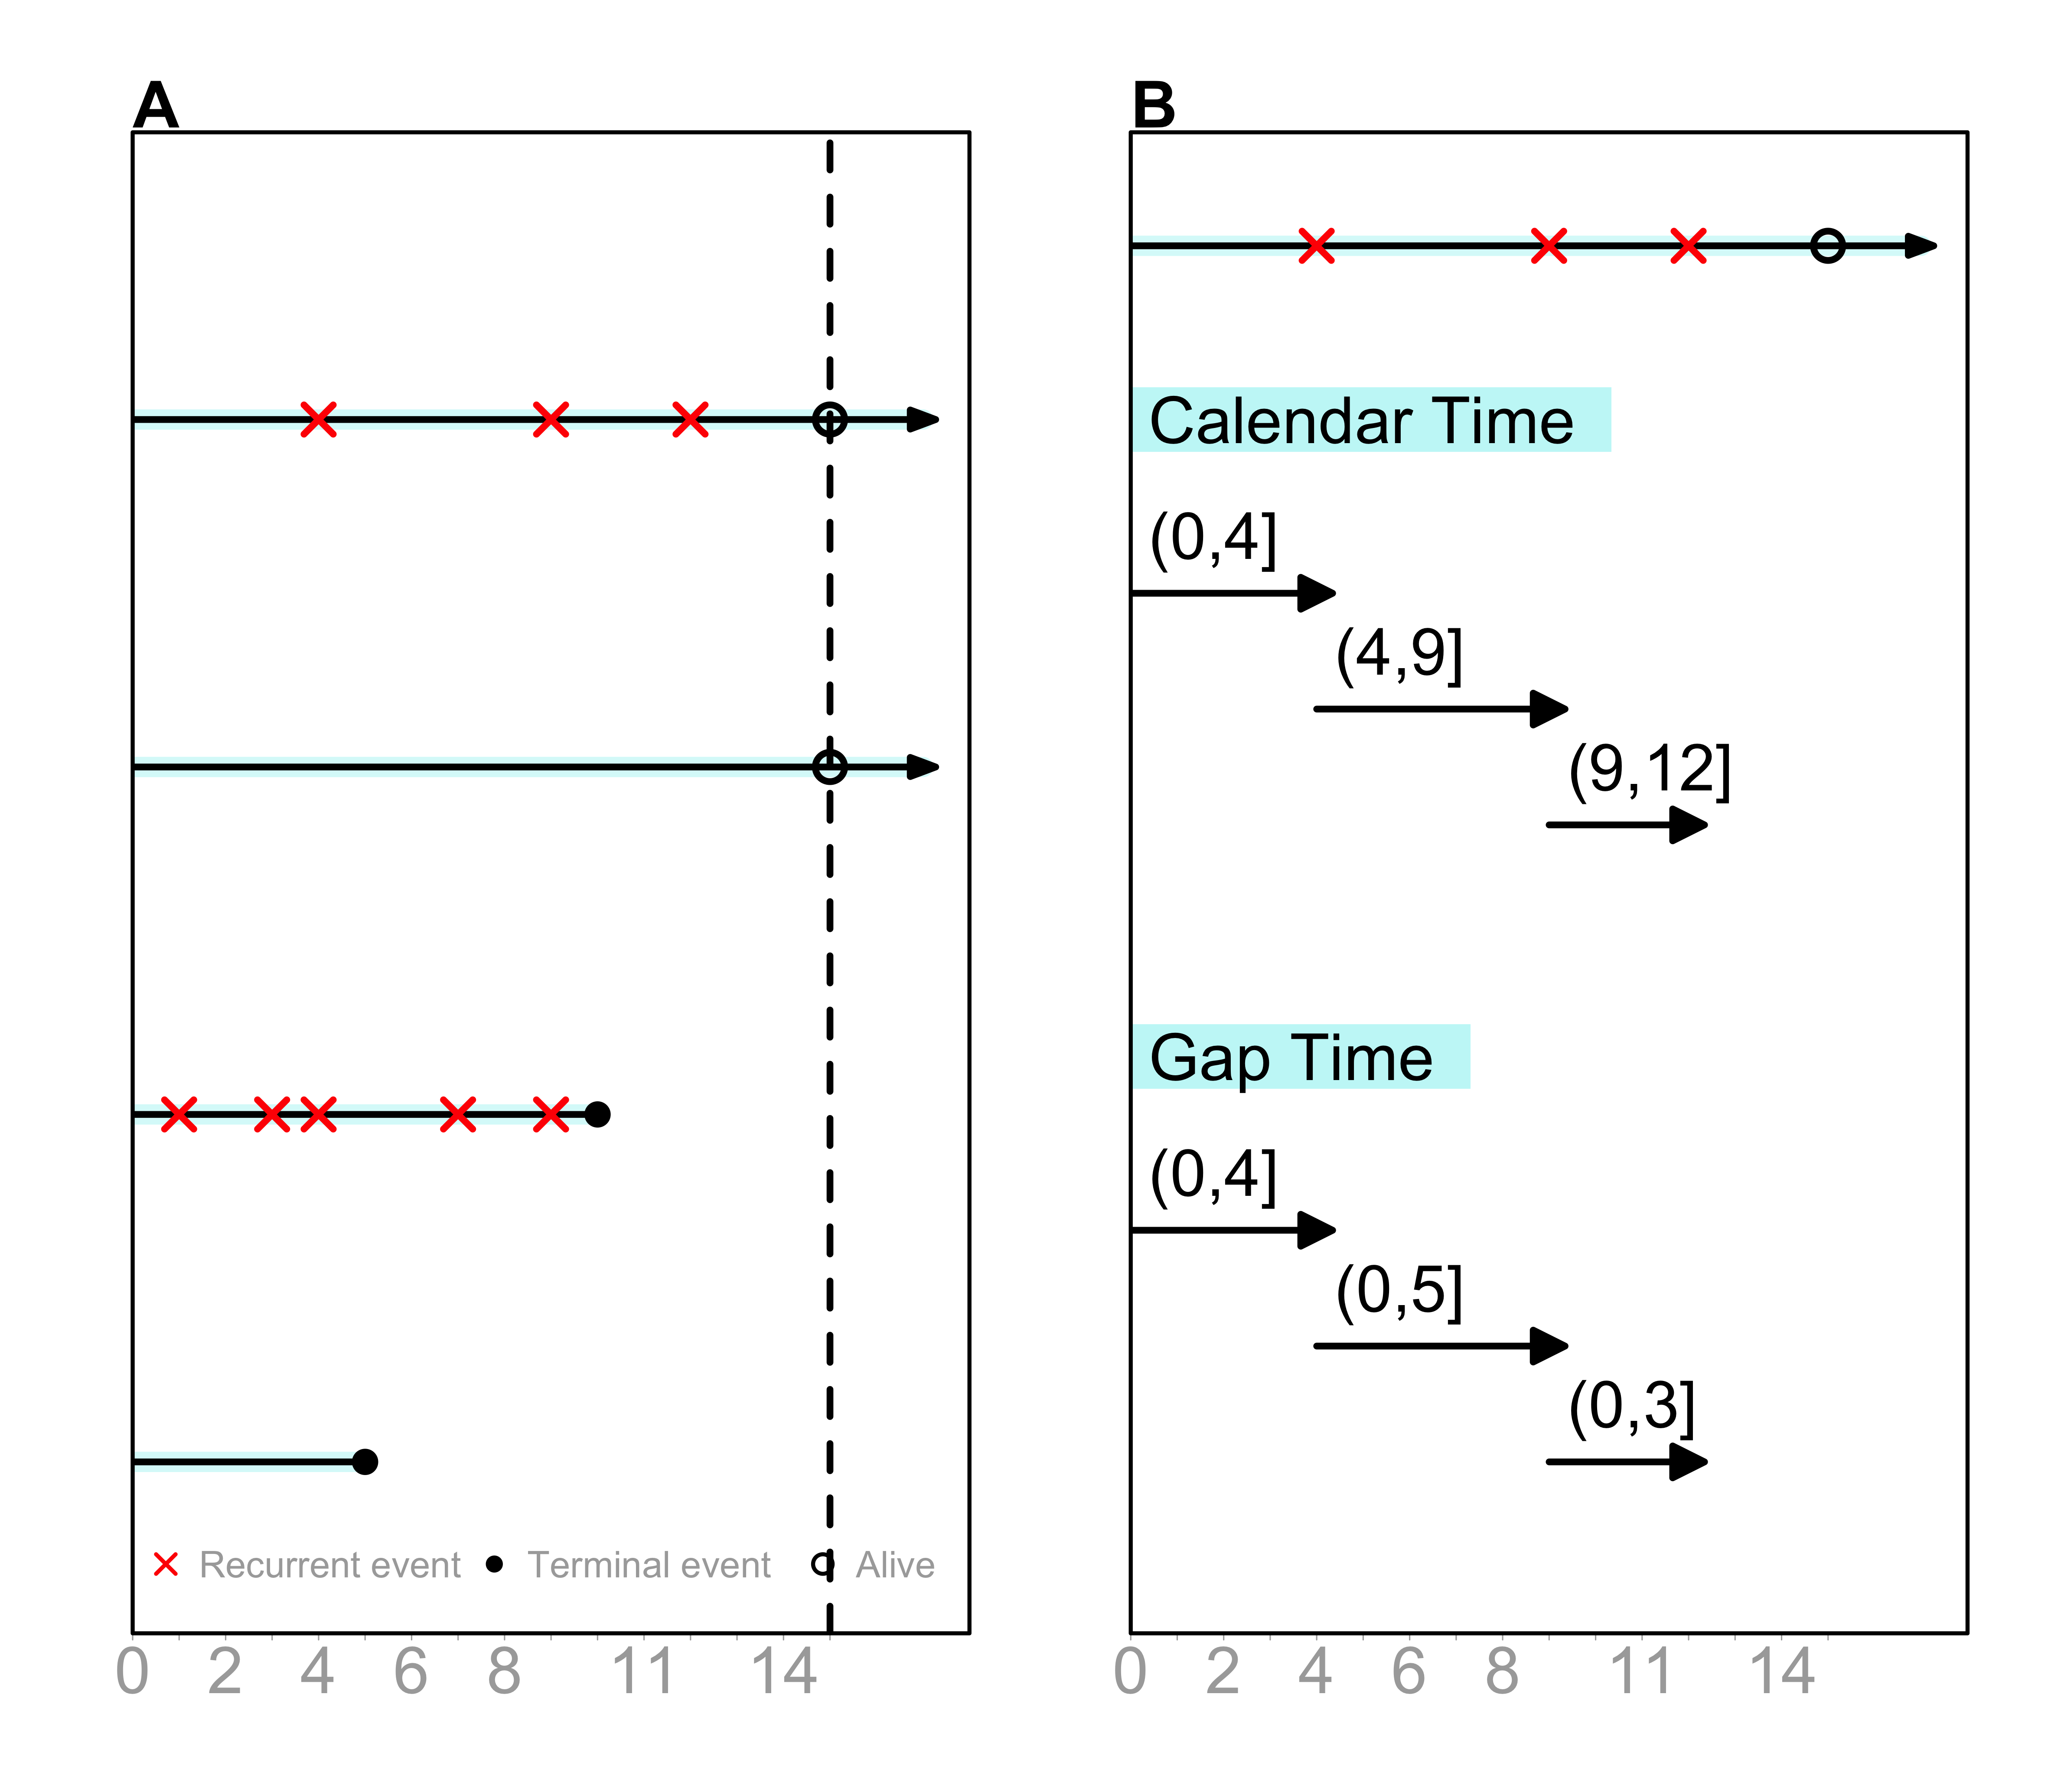
\includegraphics[width=0.9\textwidth]{Figures/Chp3_censor.png}
\caption{Illustrations of data structure and time scales. A: PE occurrences for four selected patients censored at a terminal event or the end of observed period; B: Definitions of risk intervals for calendar time and gap time.}
\label{fig:chp3_censor}
\end{figure}

\section{Joint Model Framework} \label{sec:chp3_mod}

The proposed joint model with shared parameter consists of a longitudinal submodel and an event submodel, specified separately for each type of outcomes. The two submodels are linked using a latent trajectory, which is parameterised in current value and time-dependent slope of the linear predictor. 

\subsection{Longitudinal Submodel}

We define $y_{lij}(t)=y_{li}(t_{lij})$ corresponds to the observed longitudinal outcome for $i^{th}$ ($i=1,\dots,n_l$) individual who comes from $l^{th}$ ($l=1,\dots, L$) center taken at time point $t_{lij}$ ($j=1,\dots,n_{li}$). Then the mixed effects model for $y_{lij}(t)$ takes the form

\begin{align}
&  \left \{\begin{array}{ll}
 y_{lij}(t)=m_{lij}(t)+\epsilon_{lij}(t)\\
 m_{lij}(t)=\bm{x}^T_{lij}(t)\bm{\beta}+b_l+\bm{z}^{T}_{lij}(t)\bm{U}_{li}
\end{array}\right.
\end{align}
where $m_{lij}(t)$ corresponds to the individual linear predictor of observed outcome. $\bm{x}^T_{lij}(t)$ and $\bm{z}^T_{lij}(t)$ are row-vectors of covariates with associated fixed effect coefficient $\bm{\beta}$ and random effects $\bm{U}_{li}$, respectively. The random intercept $b_l$ is set for centers by assuming $b_l \sim N(0,\sigma^2_b)$. The measurement error $\bm{\epsilon}_{li}$ is distributed as $N(\bm{0},\bm{R}_{li})$. As proposed in \cite{Laird1982}, the $\bm{U}_{li}$ are distributed as $N(\bm{0},\bm{D})$, allowing for $\bm{D}$ as an $n_{li} \times n_{li}$ positive-definite covariance matrix, independently of each other and of the $b_l$ and of the $\bm{\epsilon}_{li}$. Further simplification arises when $\bm{R}_{li}=\sigma^2\bm{I}$, where $\bm{I}$ denotes an identity matrix and $\bm{D}=\bm{\Sigma_u}$ with the variance terms ${\sigma^2_{u0}, \sigma^2_{u1}}$ and the correlation coefficient term $\rho$. 

\subsection{Event Submodel}

Let $T_{li}=min(T^{*}_{li},C_{li})$ denote terminal event time where $T^{*}_{li}$ is the so-called 'true' event time and $C_{li}$ is the corresponding censoring time. We define $t_{lik}$ as the observed time for the event submodel with $t_{lik} \leq T_{li}$ $(k \in j)$ and $d_{lik}$ as the event indicator. The individual hazard of a recurrent event using a parametric proportional hazards regression model is given by, 
\begin{align}
    h_{lik}(t)=h_{l0}(t)exp\big\{\bm{\omega}^T_{lik}(t)\bm{\gamma}+f(\bm{\beta},b_l,\bm{U}_{li},\alpha_l;t)+v_{li}\big\}
\end{align}
where $h_{lik}(t)$ denotes $h_{li}(t_{lik})$ for simplicity, $h_{l0}(t)$ is the center-specific baseline hazard, $\bm{\omega}^T_{lik}(t)$ is a row-vector of individual covariates (possibly time-dependent) with corresponding regression coefficient $\bm{\gamma}$ (also known as log hazard ratio). The longitudinal and event processes are assumed to be related via an 'association structure', which is denoted by $f(\cdot)$. In particular, center-specific $\alpha_l$ quantifies the association between the time-varying longitudinal marker and the risk of a recurrent event. Based on our preliminary analysis, we choose current value and current slope of the linear predictor as the association structure, such as

\begin{align}
&  \left \{\begin{array}{ll}
 \mbox{Current value: }f(\bm{\beta}, b_l, \bm{U}_{li}; t)=\alpha_{vl} \times m_{lik}(t)\\
 \mbox{Current slope: }f(\bm{\beta}, b_l, \bm{U}_{li}; t)=\alpha_{sl} \times \frac{d}{dt} m_{lik}(t)
\end{array}\right.
\end{align}
The term $v_{li}$ is a random effect that accounts for the correlation between recurrent events and it is assumed to follow $v_{li} \sim N(0,\sigma^2_v)$  independently. Note that $exp(v_{li})$ is also well known as the frailty term. We further assume that our longitudinal data is non-informative right censoring and the baseline hazard function is modeled with a Weibull distribution, that is $h_{l0}(t)=\delta_l t^{\delta_l-1}$ with $\delta_l$ as center-specific shape parameter. 

\subsection{Assumption}

The key assumption in our proposed joint model is the conditional independence, which means random effects $\bm{b},\bm{U}$ and $\bm{v}$ explain all the interdependence. Let $\bm{\theta}$ denote a vector of all unknown parameters, then we have expressions as followings, 


The longitudinal process is conditionally independent of the event process:
\begin{align}
   p(\bm{t}_{li},\bm{d}_{li},\bm{y}_{li}|b_l,\bm{U}_{li},v_{li};\bm{\theta})=p(\bm{t}_{li},\bm{d}_{li}|b_l,\bm{U}_{li},v_{li};\bm{\theta}) \times p(\bm{y}_{li}|b_l,\bm{U}_{li};\bm{\theta}) 
\end{align}

Recurrent events in the event process are independent of each other: 
\begin{align}
    p(\bm{t}_{li},\bm{d}_{li}|b_l,\bm{U}_{li}, v_{li};\bm{\theta})=\prod_k p(t_{lik},d_{lik}|b_l,\bm{U}_{li},v_{li};\bm{\theta})
\end{align}

Repeated measurements in the longitudinal process are independent of each other: 
\begin{align}
  p(\bm{y}_{li}|b_l,\bm{U}_{li};\bm{\theta})=\prod_j p(y_{lij}|b_l,\bm{U}_{li};\bm{\theta})  
\end{align}

\subsection{Bayesian Inference}

In this section, we specify the posterior distribution, likelihood function of event submodel and prior distributions. All posterior samplings are carried out from the new lightweight R interface \emph{CmdStanr} to \emph{Stan} (\cite{Gelman2013a}, \cite{StanManual}). In both simulation and application study, we obtain 2000 post-warmup posterior samplings via two chains and ensure the convergence by Gelman and Rubin potential scale reduction statistic $\widehat{R}$. Details of elapsed time with system information are included in Appendix \ref{app:c}.  

\subsubsection{Log posterior distribution}

Under the full conditional independence assumption, the individual log posterior distribution can be specified as

\begin{align}
    \begin{split}
        \mbox{log } p(\bm{\theta},b_l,\bm{U}_{li},v_{li}|\bm{y}_{li}, \bm{t}_{li}, \bm{d}_{li}) \propto \mbox{log } & 
        \Big[\prod_jp(y_{lij}|b_l,\bm{U}_{li},\bm{\theta})
        \times \prod_kp(t_{lik},d_{lik}|b_l,\bm{U}_{li},v_{li},\bm{\theta}) \\ & 
        \times p(b_l|\bm{\theta})p(\bm{U}_{li}|\bm{\theta})p(v_{li}|\bm{\theta})p(\bm{\theta})\Big]
    \end{split}
\end{align}

Specifically, the log likelihood function for the event submodel under two scenarios can be rewritten as

\begin{align}
&  \left \{\begin{array}{ll}
 \mbox{Calendar time scale: } \mbox{log } p(t_{lik}, d_{lik}|b_l,\bm{U}_{li},v_{li},\bm{\theta}) = d_{lik} \cdot \mbox{log } h_{li}(t_{lik}) - \int^{t_{lik}}_{t_{li(k-1)}} h_{li}(s)ds \\
 \mbox{Gap time scale: }\mbox{log } p(t_{lik}, d_{lik}|b_l,\bm{U}_{li},v_{li},\bm{\theta}) = d_{lik} \cdot \mbox{log } h_{li}(t_{lik}-t_{li(k-1)}) - \int^{t_{lik}-t_{li(k-1)}}_{0} h_{li}(s)ds
\end{array}\right.
\end{align}
where the latter integral term can be evaluated approximately by Gauss-Kronrod quadrature with Q nodes (\cite{Laurie1997}), such that 

\begin{align}
  \int_a^b h(s)ds \approx \sum^{Q}_{q=1} w_{q,scaled} \cdot h(s_{q,scaled})  
\end{align}
where $w_{q,scaled}=w_q \cdot \frac{b-a}{2}$ and $s_{q,scaled}=\frac{s_q+1}{2}\cdot(b-a)+a$ are scaled weights and locations for quadrature node $q (q=1,\dots, Q)$. The $w_q$ and $s_q$ are standardised wights and locations (also known as abscissa) on interval $[-1,1]$ and we obtain their specific values from the source code of \emph{stan\_jm} from R package \emph{rstanarm} by choosing quadrature nodes $Q=7$.

\subsubsection{Prior distributions}

We identify diffuse or weakly informative but proper priors for all unknown parameters in the proposed joint model. Let $N(\mu,\sigma^2)$ denote normal distribution with location $\mu \in \mathbb{R}$ and scale $\sigma \in \mathbb{R}^{+}$; $t(\nu,\mu,\sigma)$ denote student's t distribution with degrees of freedom $\nu \in \mathbb{R}^{+}$, location $\mu \in \mathbb{R}$ and scale $\sigma \in \mathbb{R}^{+}$; $lkjCorr(\Sigma|\eta) \propto det(\Sigma)^{\eta-1}$ represent LKJ correlation distribution, such that $\Sigma$ is a positive-definite, symmetric matrix with unit diagonal correlation matrix (i.e., a correlation matrix) with shape parameter $\eta \in \mathbb{R}^+$ (see \cite{Lewandowski2009} for details). The prior specifications for the simulation and the application are:

$$\beta_0 \sim N(0,100^2),$$
$$\beta_p \sim N(0,\phi^2_\beta), p=1,2,\dots,P,$$
$$\sigma \sim N(0,\phi^2_\sigma),$$
$$\sigma_b \sim N(0,10^2),$$
$$\sigma_{u0}, \sigma_{u1} \sim t(1,0,10),$$
$$
\begin{bmatrix}
1 & \rho \\
\rho & 1
\end{bmatrix}  \sim lkjCorr(2), $$
$$\gamma_0 \sim N(0,20^2),$$
$$\gamma_q \sim N(0,\phi^2_\gamma), q=1,2,\dots, Q,$$
$$\lambda_l \sim N(0,5^2), l=1,2,\dots,L,$$
$$\sigma_v \sim N(0,10^2)$$
where $\phi_\beta$ and $\phi_\gamma$ are standard deviations of corresponding design matrices and $\phi_\sigma$ is the standard deviation of observed longitudinal outcomes. Practically, \emph{Stan} provides an implicit parameterization of the LKJ correlation matrix density in terms of its Cholesky factor, thus we can set $L_u$ as a Cholesky factor of the correlation matrix $\Sigma=\begin{bmatrix}
1 & \rho \\
\rho & 1
\end{bmatrix}$, such that $L_u \sim \mbox{lkj\_corr\_cholesky}(2)$ implies $\Sigma = L_u \cdot L^{T}_u \sim lkjCorr(2)$. Readers who are interested in this topic can refer to \cite{Sorensen2016} for generating correlated random variables using the Cholesky decomposition. 

\subsection{Individual Prediction}

The individual prediction for the longitudinal marker at time $t$, can be generated from the posterior predictive distribution 
\begin{align} \label{eq:indpred}    
    p(\tilde{y}_{lij}(t)|\mathcal{D})=\int\int\int p(\tilde{y}_{lij}(t)|b_l,\bm{U}_{li},\bm{\theta}) p(b_l,\bm{U}_{li},\bm{\theta}|\mathcal{D}) \,  db_l \,  d\bm{U}_{li} \, d\bm{\theta} 
\end{align}
where $\mathcal{D}=\{\bm{y}_{li},\bm{t}_{li},\bm{d}_{li}; l=1,\dots,L, i=1,\dots,n_l\}$ is the entire collection of data. To compute Equation (\ref{eq:indpred}), we can draw samplings from $p(y_{lij}(t)|b_l^{(m)},\bm{U}_{li}^{(m)},\bm{\theta}^{(m)})$, such that ${b_l^{(m)}, \bm{U}_{li}^{(m)}}$ and $\bm{\theta}^{(m)}$ are the $m^{th}(m=1,\dots,M)$ HMC draws from the joint posterior distribution of $p(b_l,\bm{U}_{li},\bm{\theta}|\mathcal{D})$ as 
\begin{align} \label{eq:indpred2}
  p(\tilde{y}_{lij}(t)|\mathcal{D}) \approx \frac{1}{M} \sum_{m=1}^{M} p(\tilde{y}_{lij}(t)|b_l^{(m)},\bm{U}_{li}^{(m)},\bm{\theta}^{(m)},\mathcal{D}).   
\end{align}
In parallel, for $i^{th}$ individual who has $n^*_{li}(n^*_{li}=0,1,2,\dots)$ recurrent events up to the time $t$, it might be of interest to look beyond and predict the probability of next event-free outcome in the time frame $(t,t']$ with $t'=t+\Delta t$. For this cause, the conditional survival (PE-free) probability can be written as,
\begin{align} \label{eq:cond.surv}
    \begin{split}
        S_{li}(t'|t) & = p(t_{n^*_{li}+1} \geq t'|t_{n^*_{li}+1} > t, \mathcal{D})  \\
                    & = \int\int\int\int p(t_{n^*_{li}+1} \geq t'|t_{n^*_{li}+1} > t, b_l,\bm{U}_{li},v_{li},\bm{\theta},\mathcal{D}) \\
                    & \cdot p(b_l, \bm{U}_{li}, v_{li}, \bm{\theta} |t_{n^*_{li}+1} > t, \mathcal{D}) \, db_l \, d\bm{U}_{li} \, dv_{li} \, d\bm{\theta} \\
        & \approx \frac{1}{M} \sum_{m=1}^{M} exp\Big[ -\int_t^{t'} h\big(s|b_l^{(m)},\bm{U}_{li}^{(m)},v_{li}^{(m)},\bm{\theta}^{(m)}\big) ds \Big]
    \end{split}
\end{align}
where the integration respect to \{$b_l,\bm{U}_{li}, v_{li}, \bm{\theta}$\} is approximated using Monte Carlo method from their posterior samples. The comprehensive derivation of Equation (\ref{eq:cond.surv}) can be found in Appendix \ref{app:c}. The integral term of $\int_{t}^{t'}h(s|\cdot)ds$ can be approximated by Gauss-Kronrod with Q=15 quadrature nodes. The 2.5\% and 97.5\% quantiles of posterior draws from Equation (\ref{eq:cond.surv}) can be obtained as the credible intervals for the predictive probability. 

\subsection{Predictive Performance}

To assess the predictive performance, we employ area under receiver operating characteristic curve (hereafter, AUC) for discrimination (discriminate between individuals who will experience the next recurrent event from subjects who will not) and predictive error for calibration (how well the model predicts the observed event probability). We calculate time-dependent AUC and predictive error under squared loss function based on source code \emph{predictive\_accuracy.stanjm} from R package \emph{rstanarm} and some other nice references (\cite{Andrinopoulou2018}, \cite{Andrinopoulou2021}). The details are described in Table \ref{tab:chp3_auc}.

\begin{table}[H]
\centering \small
\caption{Algorithm for time-dependent AUC and mean predictive error} \label{tab:chp3_auc}
\begin{tabular}{p{14cm}} 
 \toprule
 \textbf{Time-dependent AUC}\\
 \midrule
  \begin{enumerate}
      \item Define individual-specific start time $t_i=\mbox{tstart}_i$ and a common future stop time $t'$. To conform the prediction data, we only include individuals who are still at risk of the event at $t$. For longitudinal data, we adopt observations observed until $t_i$. 
      \item Calculate event-free ('survival') probability at $t'$ and observed $\mbox{tstop}_i$ for each individual based Equation (\ref{eq:cond.surv}) to obtain $S_i(t'|t_i)$ and $S_i(\mbox{tstop}_i|t_i)$
      \item Sort individuals by their observed $\mbox{tstop}$ in an increasing order and group each two by combinations without replacement. 
      \item AUC is calculated by accounting for weights caused by censoring conditions. For each combation $c=1,\dots,C$, assume that $\mbox{tstop}_i < \mbox{tstop}_j$:
        \begin{itemize}
            \footnotesize
            \item If only individual $i$ is censored at $t'$, which means $\mbox{tstop}_i \leq t'$ \& $\mbox{status}_i=0$, then weight $w=1-S_i(\mbox{tstop}_i|t_i)$
            \item If only individual $j$ is censored at $t'$, which means $\mbox{tstop}_j \leq t'$ \& $\mbox{status}_j=0$, then weight $w=S_j(\mbox{tstop}_j|t_j)$
            \item If both individuals are censored at $t'$, then weight $w=\big(1-S_i(\mbox{tstop}_i|t_i)\big) \times S_j(\mbox{tstop}_j|t_j)$
            \item If it does not belong to above cases, $w=1$
            \item Let $S_i=S_i(t'|t_i), S_j=S_j(t'|t_j)$, compute $A_c=I_{S_i<S_j} \cdot w$; $D_c=I_{S_i>S_j} \cdot w$; $T_c=I_{S_i=S_j} \cdot w$, where $I_x$ denotes a indicator function with 1 when $x$ is true and 0, otherwise. 
        \end{itemize}
      \item Repeat Step 4 until $C$ times
      \item $\mbox{AUC}=\sum_{c=1}^C \big(\frac{A_c+0.5 \cdot T_c}{A_c + D_c + T_c}\big)$
   \end{enumerate}\\
    \hline
 \textbf{Time-dependent mean predictive error (MPE)}\\
 \midrule
 \begin{enumerate}
     \item  For each individual $i (i=1,\dots,N)$: 
         \begin{itemize}
         \footnotesize
             \item If individual $i$ died or censored after $t'$, $\mbox{Error}_i=(1-S_i)^2$
             \item If individual $i$ died before $t'$, $\mbox{Error}_i=(0-S_i)^2$
             \item If individual $i$ censored before $t'$, $\mbox{Error}_i=S_i(\mbox{tstop}_i|t_i) \times (1-S_i)^2+\big(1-S_i(\mbox{tstop}_i|t_i)\big) \times (0-S_i)^2$
         \end{itemize}
    \item Mean Predictive Error (MPE)=$\frac{\sum_{i=1}^{N}\mbox{Error}_i}{N}$
 \end{enumerate}\\
 \bottomrule
 \hline
\end{tabular}
\end{table}

\subsection{Model Selection}

We allude to the leave-one-out (LOO) cross-validation for model choice, which in its own words is the method for estimating pointwise out-of-sample prediction accuracy from the log-likelihood evaluated at the posterior simulations of the parameter values. \cite{Vehtari2017} developed an efficient computation for LOO using Pareto-smoothed importance sampling (PSIS) to lay out fast and stable computations for LOO. PSIS-LOO is demonstrated to be even more robust than asymptotic widely applicable information criterion (WAIC) (\cite{Watanabe2010}), which is a recent popular measure of predictive accuracy. We implement the computations of LOO information criterion (LOOIC) via R package \emph{loo} (v2.3.1, \cite{Vehtari2020}) by extracting log likelihoods from posterior samplings.  

The PSIS estimate of expected log pointwise predictive density (elpd) is 
\begin{align} \label{eq:loo}
    \widehat{\mbox{elpd}}_{\mbox{psis-loo}}=\sum_{l=1}^{L}\sum_{i=1}^{n_l}log\Big(\frac{\sum_{s=1}^S w^s_{li}p(y_{li}|\theta^s)}{\sum_{s=1}^S w^s_{li}} \Big)
\end{align}
 where $w^s_{li}$ denotes weights at iteration $s$, $p(y_{li}|\theta^s)$ denotes likelihood function at $s$. As with WAIC, we define LOOIC as $-2$ times the Equation (\ref{eq:loo}) so as to be on the deviance scale. Analogously, the model with smaller LOOIC value indicates the better goodness of fit. 
 
\section{Simulation} \label{sec:chp3_sim}

We simulate a total of four hierarchical data sets and fit to corresponding proposed joint models, with the aim to assess the performance of each proposed joint model in a comparison of the two-stage approach. Four proposed joint models are summarized as: i) joint model with current slope as the association structure and gap time as the time scale (hereafter, Slope+Gap); ii) joint model with current slope as the association structure and calendar time as the time scale (hereafter, Slope+Calendar); iii) joint model with current value as the association structure and gap time as the time scale (hereafter, Value+Gap); iv) joint model with current value as the association structure and calendar time as the time scale (hereafter, Value+Calendar). 

\begin{table}[H]
\small\centering
\caption{Simulation progress} \label{tab:chp3_sim}
\begin{tabular}{p{14cm}} 
 \toprule
 {\normalsize \bf Simulation algorithm} \\
 \midrule
  \textbf{\emph{Random effects}}\\
     Simulate $b_l \sim N(0,\sigma_b^2)$, $\bm{U_i}=(U_{0i},U_{1i})^T \sim N(\bm{0},\bm{\Sigma}_u)$, and $\bm{\Sigma}_u$ is the covariance matrix with the variance terms $\sigma^2_{u0}, \sigma^2_{u1}$ and the correlation coefficient term $\rho$ \\
   \midrule 
   
   \bf Event Process
    \hspace{0.5cm} \
    \begin{enumerate}
        \item \textbf{\emph{Terminal event}} 
            \begin{itemize}
                \item Simulate $\omega_1 \sim \mbox{Bernoulli}(0.5), \omega_2 \sim N(0,1), v_i \sim N(0,\sigma^2_v), u_i \sim \mbox{Uniform}(0,1)$
                \item Let $A=\gamma_0+\gamma_1\omega_1+\gamma_2\omega_2$
                \item Define hazard function with Weibull as the baseline hazard, that is $h_{i}(t)=\delta_l t ^{\delta_l-1} exp(A)$
                \item Cumulative hazard function $H_i(t)=\int_{0}^{t}h_{i}(s)ds$
                \item Solve $t$ from equation $H_i(t)+log(u_i)=0$
                \item Terminal time $T_i=min(t,t_{\mbox{max}})$, where maximum follow-up time $t_{\mbox{max}}=10$ years
            \end{itemize}
        \item \textbf{\emph{Recurrent event}}
            \begin{itemize}
                 \item Let $f(\beta,b_l,\bm{U}_i;t)=\alpha_{vl} \cdot m_{ik}(t)/\alpha_{sl} \cdot m'_{ik}(t)$, where $m_{ik}(t)=\beta_0+\beta_1 t+\beta_2 t^2+b_l+U_{0i}+U_{01} \cdot t$
                \item Hazard function of $k^{th}$ event: $h_{ik}(t)=\delta_l t ^{\delta_l-1} exp(A+ f(\beta,b_l,\bm{U}_i;t) + v_i)$
                \item Set starting point: $\mbox{tstart}_{i0}=0$
                \item In each loop $k=1,\dots,K$, generate $u_{ik}\sim \mbox{Uniform}(0,1)$
                \item If time scale is set as gap: Solve $\Delta t_{ik}$ from equation $H_i(\Delta t_{ik})+log(u_{ik})=0$, where $H_i(\Delta t_{ik})=\int_{0}^{\Delta t_{ik}}h_{ik}(s)ds=$
               $\int_{0}^{\Delta t_{ik}}\delta_l s^{\delta_l-1}exp\big(A+f(\beta,b_l,\bm{U}_i;s+\mbox{tstart}_{ik})+v_i\big)ds$
                \item If time scale is set as calendar: Solve $\Delta t_{ik}$ from equation $H_i(\Delta t_{ik})+log(u_{ik})=0$, where $H_i(\Delta t_{ik})=\int_{0}^{\Delta t_{ik}}h_{ik}(s)ds=$ 
               $\int_{0}^{\Delta t_{ik}}\delta_l (s+\mbox{tstart}_{ik})^{\delta_l-1}exp\big(A+f(\beta,b_l,\bm{U}_i;s+\mbox{tstart}_{ik})+v_i\big)ds$
             \item Update $\mbox{tstart}_{ik}=\mbox{tstart}_{i(k-1)}+\Delta t_{ik}+ \mbox{28 days}$, $\mbox{tstop}_{i(k-1)}=\mbox{tstart}_{i(k-1)}+\Delta t_{ik}$ until $\mbox{tstart}_{ik}$ reaches up to $T_i$
            \end{itemize}
    \end{enumerate}\\
      \midrule 
   \textbf{Longitudinal Process}\\ 
   %\hspace{0.5cm} \textbf{\emph{Longitudinal marker}}: \\
    Once $\mbox{tstop}_{i(k-1)}$ is obtained from the previous step, we adjust $t_{ij}=\mbox{tstop}_{i(k-1)}$ for $j=2,\dots,K+1$ and set $t_{ij}=0$ for $j=1$, such that $y_{ij}=m_{ij}(t_{ij})+\epsilon_{ij}$,
  where $\epsilon_{ij} \sim N(0,\sigma^2)$\\
      \bottomrule
\end{tabular}
\end{table}

We simulate each data set consisting of an average of 480 individuals who are from $L=6$ centers for 50 replicates for each proposed joint model. The data generating algorithm is shown in Table \ref{tab:chp3_sim}. It is worth noting that we add a fixed time window (28 days) to mimic the real case by accounting for patients' recovery time. Comparisons between estimate and true value of each parameter are displayed in Figure \ref{fig:chp3_est1} and Figure \ref{fig:chp3_est2}. We observe that both joint model and two-stage approaches yield to reasonable fitting performance. Nonetheless, there exists the need to investigate both approaches in a real data example, which will be discussed in the next section. Details for explicit true values, estimates are described in Appendix \ref{app:c}.  

\begin{figure}[ht] 
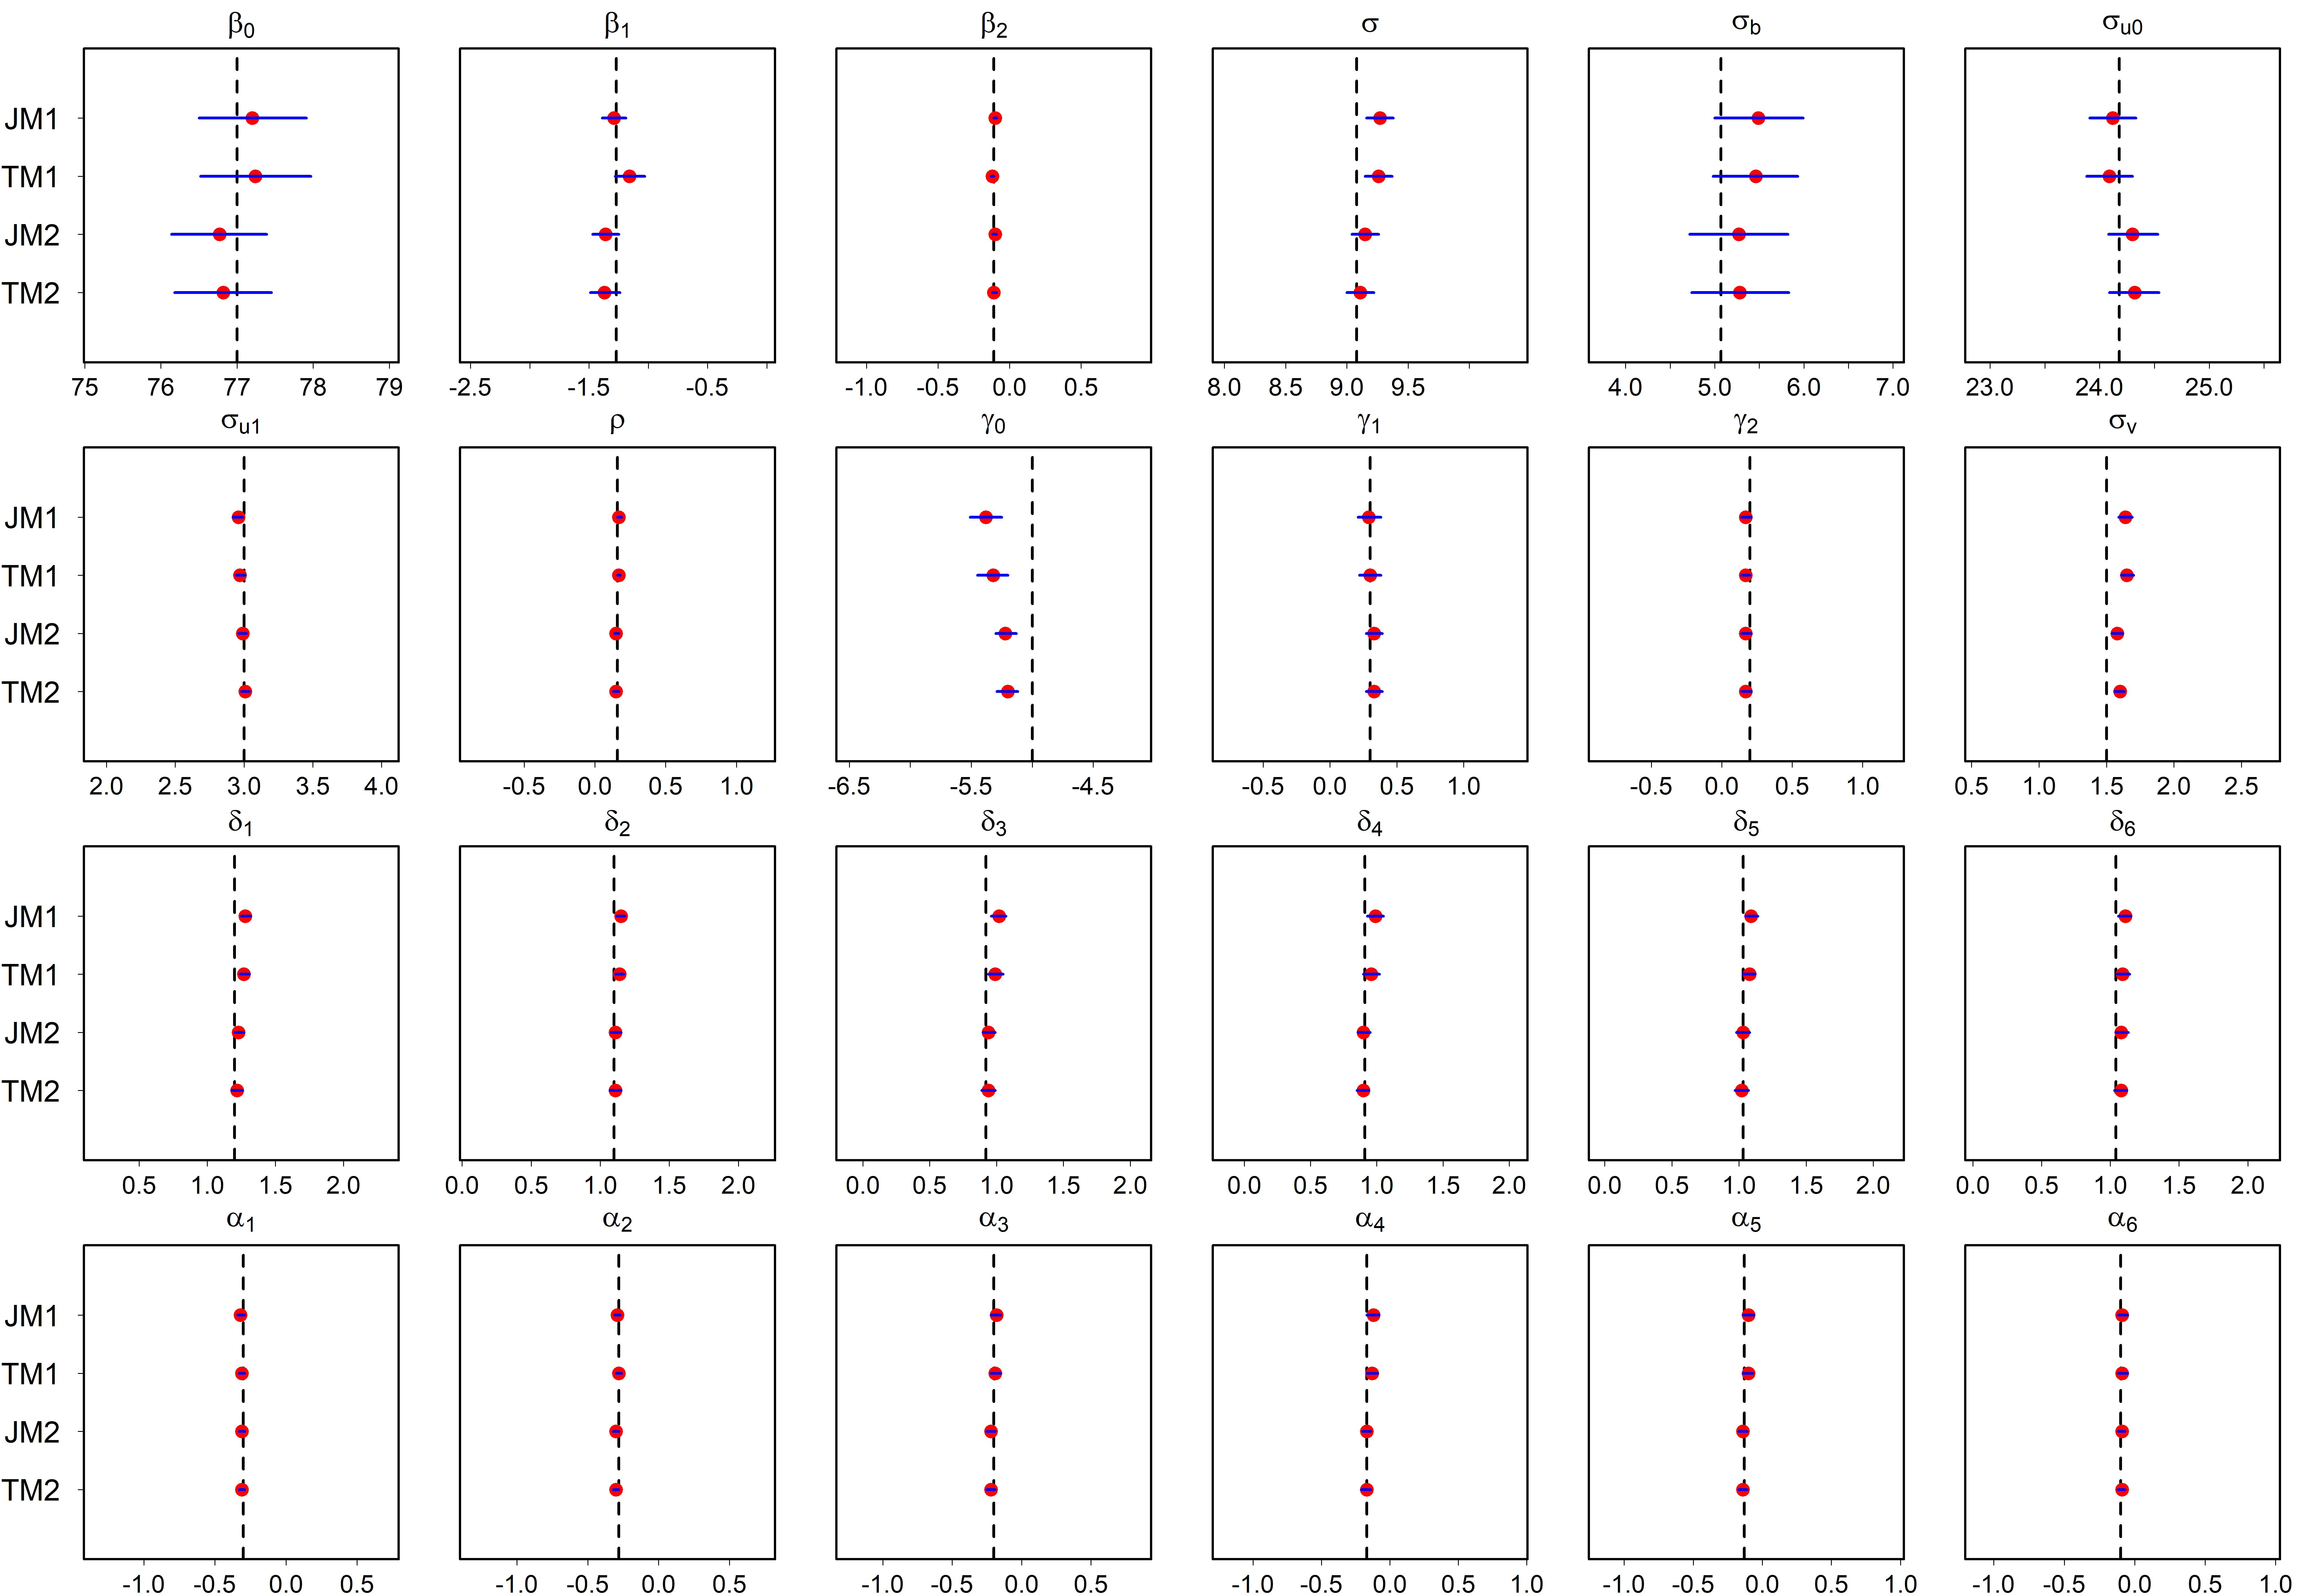
\includegraphics[width=\textwidth]{Figures/Chp3_sim_1.jpg} 
\caption{Simulation results based on 50 replicates with true value (dashed vertical line), posterior mean estimates (red dot) and corresponding 95\% confidence interval (blue line). JM1: Joint model Slope+Gap; TM1: Two-stage model Slope+Gap; JM2: Joint model Slope+Calendar; TM2: Two-stage model Slope+Calendar}
\label{fig:chp3_est1}
\end{figure}

\begin{figure}[ht] 
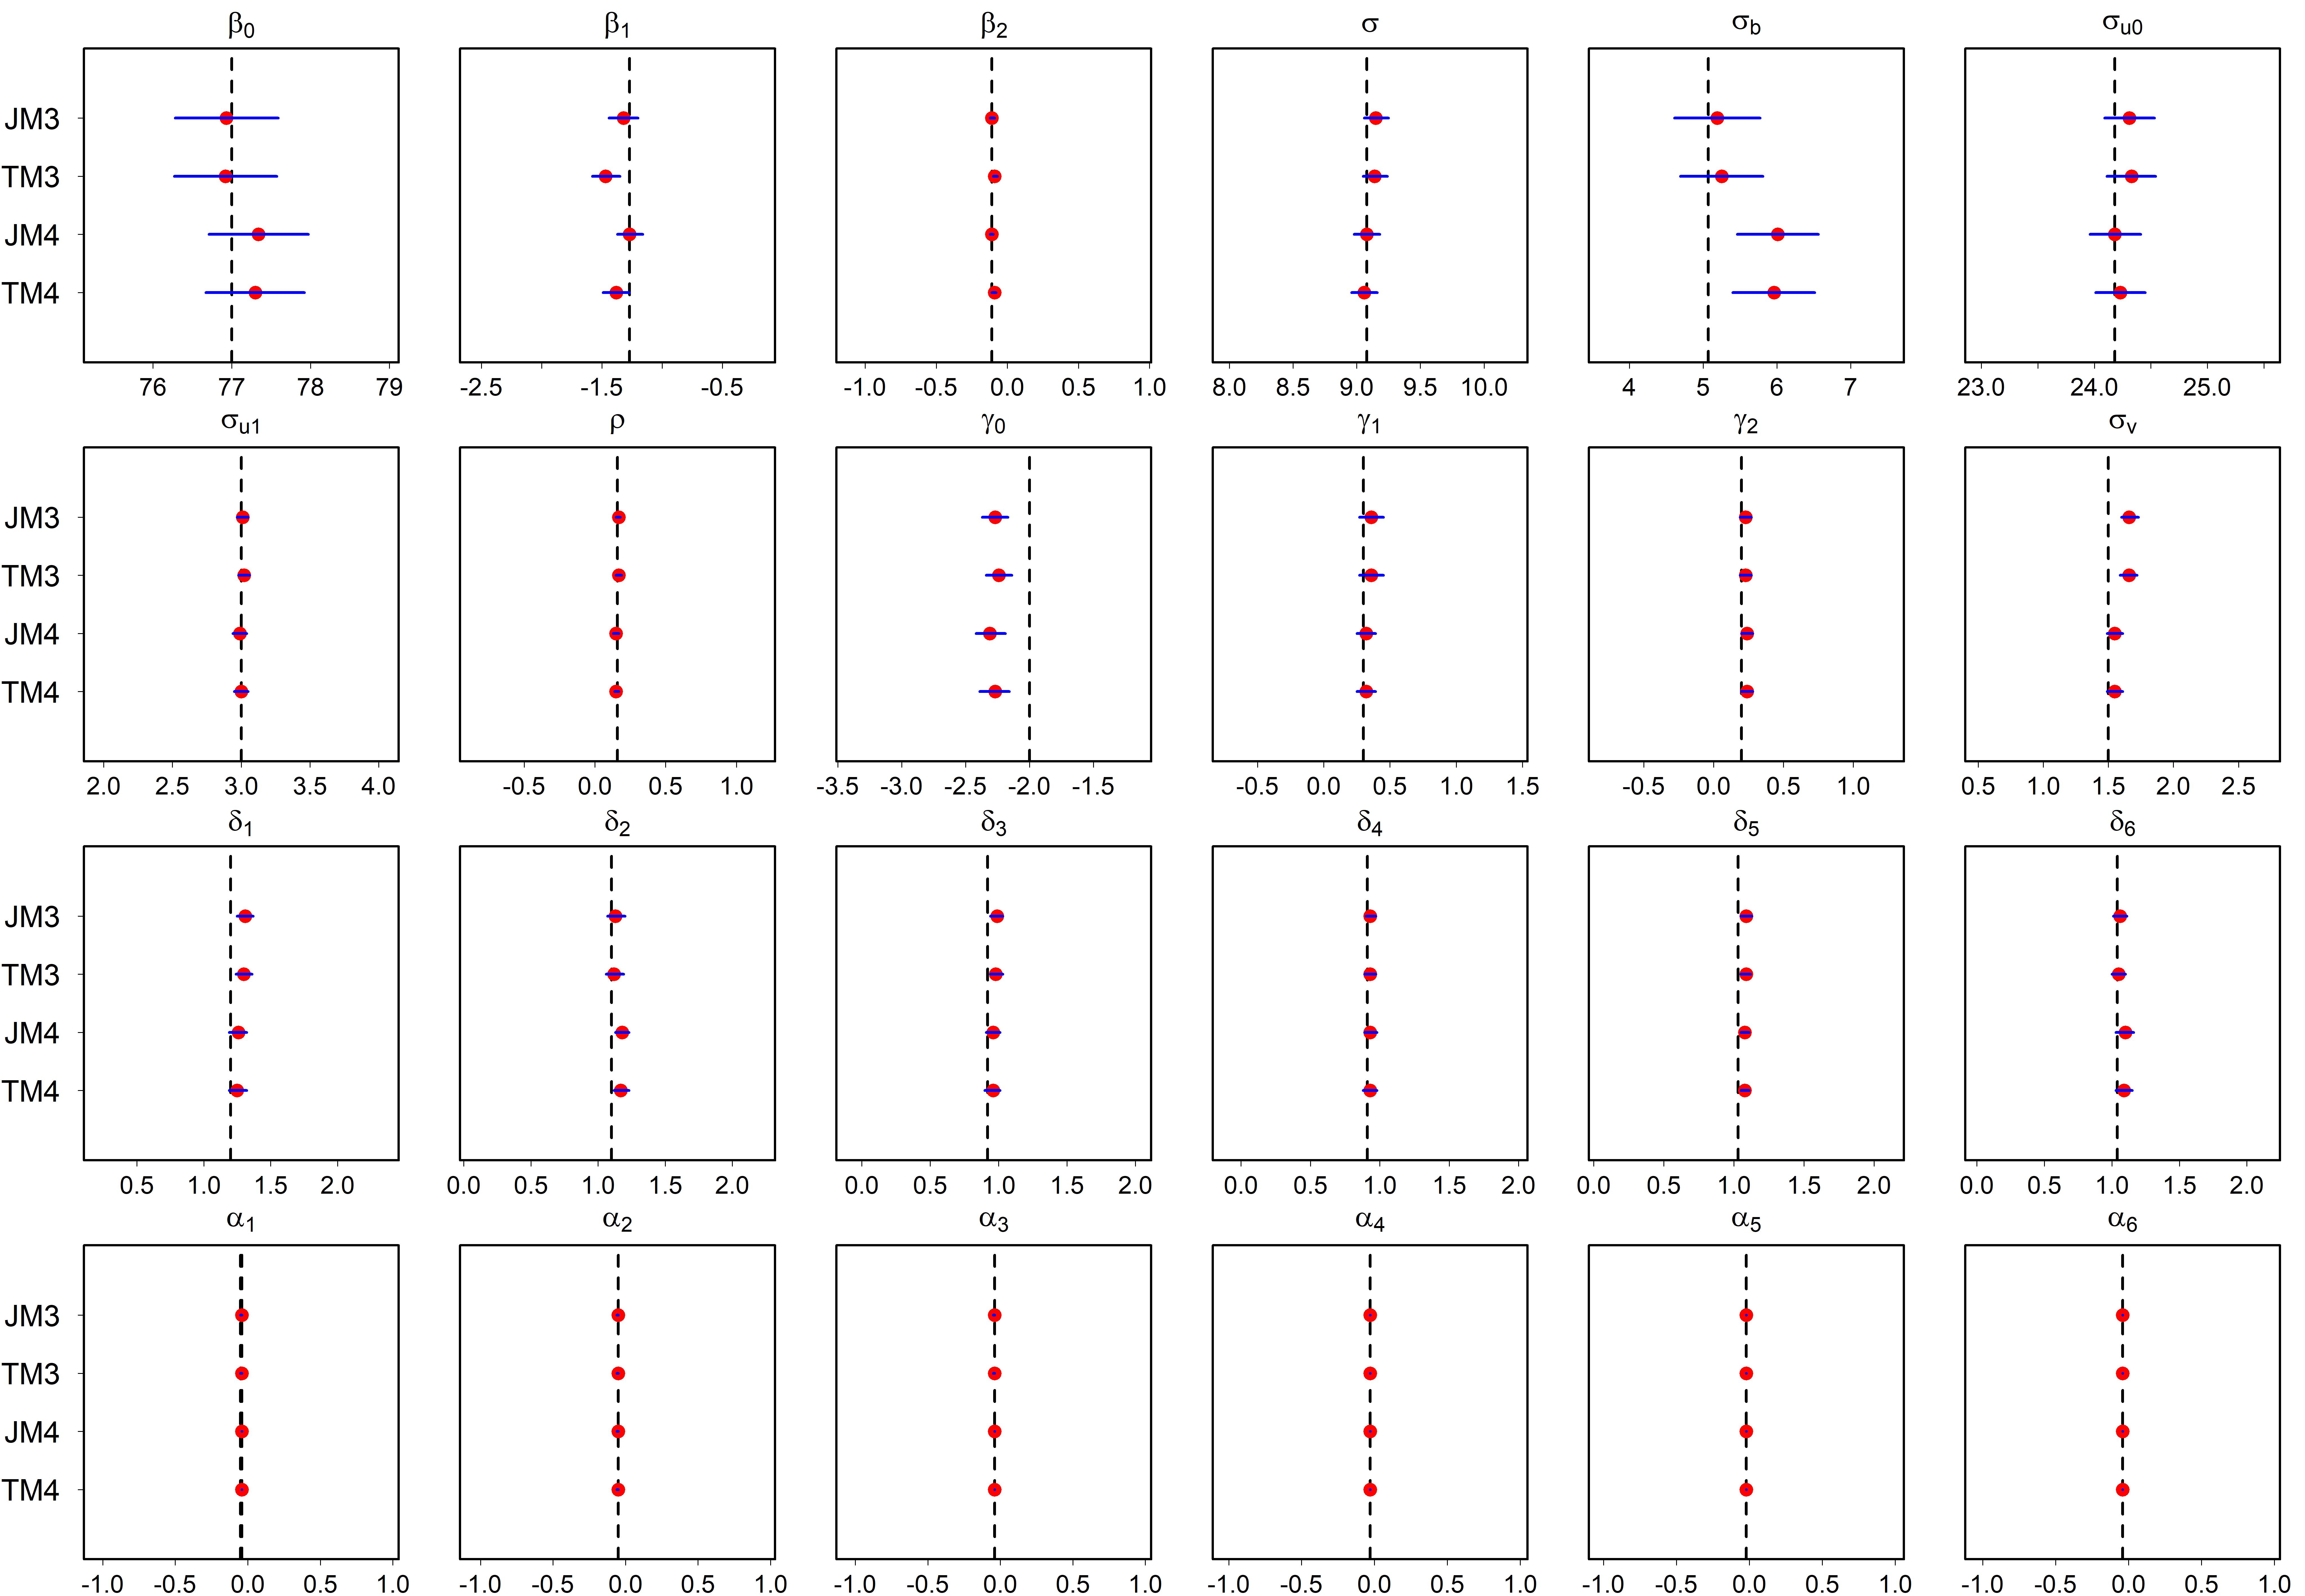
\includegraphics[width=\textwidth]{Figures/Chp3_sim_2.jpg}
\caption{Simulation results based on 50 replicates with true value (dashed vertical line), posterior mean estimates (red dot) and corresponding 95\% confidence interval (blue line). JM3: Joint model Value+Gap; TM3: Two-stage model Value+Gap; JM4: Joint model Value+Calendar; TM4: Two-stage model Value+Calendar}
\label{fig:chp3_est2}
\end{figure}

\section{Application} \label{sec:chp3_app}

In this section, we illustrate our motivating multi-center CF study, which tracked the lung trajectory and corresponding covariates of patients since 1997 by US CF Foundation Registry. Our study was approved by the Institutional Review Boards at Cincinnati Children’s Hospital Medical Center and University of Cincinnati.

The details of data cleaning process are described in Appendix \ref{app:c}. The final cleaned data we obtained is of 440 patients, which 178 (40.45\%) patients never encounter PE, 7 (1.59\%) patients experience PE only once, 255 (57.95\%) patients experience recurrent events during the follow-up period. Descriptive statistics by centers are summarized in Table \ref{tab:chp3_dem}, of which includes: i) demographic summary, such as Gender, Genotype, Birth cohort; ii) the first recorded covariates, such as baseline age and baseline ppFEV1; iii) binary time-varying measures on insurance use, microbiology (infection with pa or MRSA) and \emph{CF-related diabetes mellitus} (cfrd). The time since baseline is utilized as the time scale for analysis. The category levels of birth cohort are computed by quartile 0-25\%, 25\%-50\%, 50\%-75\% and 75\%-100\%, respectively. This covariate may offer some remedies for biases induced by left-truncation from review year 2003. To account for irregular visit due to disease severity, we have included numbers of PEs and outpatient visits within the year prior to a given clinical encounter as predictors. Trajectory in Figure \ref{fig:chp3_traj} displays the heterogeneous nature of lung function and recurrent feature of PE over the life span. We note that PE events are more likely to appear when the averaged values of ppFEV1 are low.   

\begin{table}[H]
  \footnotesize\sf\centering
  \captionsetup{justification=centering}
   \caption{Demographic clinical summary across centers} \label{tab:chp3_dem}
    \begin{threeparttable}
 \begin{tabular}{lcccccc}
    \toprule
  & \textbf{\specialcell{Center 1\\(N=74)}} & \textbf{\specialcell{Center 2\\(N=70)}} & \textbf{\specialcell{Center 3\\(N=75)}} & \textbf{\specialcell{Center 4\\(N=75)}} & \textbf{\specialcell{Center 5\\(N=72)}} & \textbf{\specialcell{Center 6\\(N=74)}} \\
 \midrule
\rowcolor{Gainsboro!60}
 \multicolumn{7}{l}{\textbf{Baseline age (years)}} \\[2pt]
 \hspace{0.5cm} \specialcell{Mean; Median\\(Min - Max)} &  \specialcell{19.0; 17.0\\(6.08 - 47.6)} & \specialcell{29.4; 21.9\\ (17.7 - 79.8)} & \specialcell{15.7; 13.5\\ (6.11 - 63.9)} & \specialcell{17.7; 14.7\\ (6.04 - 53.4)} & \specialcell{11.3; 10.6\\ (6.02 - 34.6)} &	\specialcell{17.4; 15.0\\ (6.01 - 51.9)}\\
\rowcolor{Gainsboro!60}
 \multicolumn{7}{l}{\textbf{Baseline ppFEV1}} \\[2pt]
 \hspace{0.5cm} \specialcell{Mean; Median\\(Min - Max)} & \specialcell{77.4; 79.2\\ (16.2 - 144)} & \specialcell{64.7; 65.8\\ (25.3 - 111)} & \specialcell{80.5; 83.5\\ (23.7 - 134)}	& \specialcell{82.2; 88.7\\ (19.7 - 117)}	& \specialcell{80.4; 85.8\\ (18.3 - 129)} & \specialcell{79.6; 80.4 \\ (19.6 - 129)}\\
 \rowcolor{Gainsboro!60}
 \multicolumn{7}{l}{\textbf{Gender}} \\[2pt]
 \hspace{0.5cm} Female & 23 (31.1\%) & 31 (44.3\%) & 31 (41.3\%) & 30 (40.0\%) & 24 (33.3\%) & 25 (33.8\%)\\ 
 \hspace{0.5cm} Male & 51 (68.9\%) & 39 (55.7\%) & 44 (58.7\%) & 45 (60.0\%) & 48 (66.7\%) & 49 (66.2\%)\\
 \rowcolor{Gainsboro!60}
 \multicolumn{7}{l}{\textbf{Genotype (F508del)}} \\[2pt]
 \hspace{0.5cm} Neither/Unknown & 30 (40.5\%) &	14 (20.0\%) & 10 (13.3\%) &	17 (22.7\%) & 14 (19.4\%) & 13 (17.6\%)\\
 \hspace{0.5cm} Homozygous & 11 (14.9\%) & 22 (31.4\%) & 40 (53.3\%) & 28 (37.3\%) & 30 (41.7\%) &	28 (37.8\%)\\
 \hspace{0.5cm} Heterozygous & 33 (44.6\%) & 34 (48.6\%) & 25 (33.3\%) & 30 (40.0\%) & 28 (38.9\%) & 33 (44.6\%)\\
 \rowcolor{Gainsboro!60}
  \multicolumn{7}{l}{ \textbf{Birth cohort}} \\[2pt]
 \hspace{0.5cm} $<1988$ & 16 (21.6\%) &	26 (37.1\%) & 20 (26.7\%) &	28 (37.3\%) & 5 (6.9\%) & 30 (40.5\%)\\
 \hspace{0.5cm} $[1988,1993)$ & 14 (18.9\%) & 21 (30.0\%) &	13 (17.3\%) &	19 (25.3\%) & 20 (27.8\%) & 13 (17.6\%)\\
 \hspace{0.5cm} $[1993,1998)$ & 12 (16.2\%) & 23 (32.9\%) &	13 (17.3\%) &	11 (14.7\%) & 19 (26.4\%) & 16 (21.6\%)\\
 \hspace{0.5cm} $>1998$ & 32 (43.2\%) &	0 (0\%)	& 29 (38.7\%) &	17 (22.7\%)&	28 (38.9\%) & 15 (20.3\%)\\
 \rowcolor{Gainsboro!60}
 \multicolumn{7}{l}{\textbf{Insurance use}} \\[2pt]
 \hspace{0.5cm} At baseline & 44 (59.5\%) & 8 (11.4\%) & 49 (65.3\%) &	58 (77.3\%) & 33 (45.8\%) & 37 (50.0\%)\\
 \hspace{0.5cm} Ever during follow-up & 53 (71.6\%) & 17 (24.3\%) & 70 (93.3\%) &	68 (90.7\%) & 48 (66.7\%) &	50 (67.6\%)\\
 \rowcolor{Gainsboro!60}
 \multicolumn{7}{l}{\textbf{Pseudomonas aeruginosa (pa)}} \\[2pt]
 \hspace{0.5cm} Baseline & 19 (25.7\%) & 15 (21.4\%) & 18 (24.0\%) & 22 (29.3\%) & 15 (20.8\%) & 17 (23.0\%)\\
 \hspace{0.5cm} Ever follow-up & 36 (48.6\%) & 41 (58.6\%) & 49 (65.3\%) & 47 (62.7\%) & 54 (75.0\%) & 47 (63.5\%)\\
 \rowcolor{Gainsboro!60}
 \multicolumn{7}{l}{\textbf{Methicillin-resistant Staphylococcus aureus (MRSA)}} \\[2pt]
 \hspace{0.5cm} At baseline & 18 (24.3\%) & 2 (2.9\%) & 11 (14.7\%) & 5 (6.7\%) & 7 (9.7\%) & 3 (4.1\%)	\\
 \hspace{0.5cm} Ever during follow-up & 28 (37.8\%) & 19 (27.1\%) & 41 (54.7\%) & 21 (28.0\%) &	37 (51.4\%) & 30 (40.5\%) \\
 \rowcolor{Gainsboro!60}
  \multicolumn{7}{l}{\textbf{CF-related diabetes mellitus (cfrd)}} \\[2pt]
 \hspace{0.5cm} At baseline & 9 (12.2\%) &	16 (22.9\%) & 6 (8.0\%) & 8 (10.7\%) & 7 (9.7\%) & 7 (9.5\%)\\
 \hspace{0.5cm} Ever during follow-up & 22 (29.7\%) & 24 (34.3\%) & 32 (42.7\%) &	33 (44.0\%) & 23 (31.9\%) & 33 (44.6\%)\\
 \rowcolor{Gainsboro!60}
  \multicolumn{7}{l}{\textbf{On Enzymes}}\\[2pt]
 \hspace{0.5cm} At baseline & 53 (71.6\%) & 58 (82.9\%) & 38 (50.7\%) & 27 (36.0\%) & 30 (41.7\%) & 25 (33.8\%)\\
 \hspace{0.5cm} Ever during follow-up & 60 (81.1\%) & 61 (87.1\%) & 68 (90.7\%) &	69 (92.0\%) & 71 (98.6\%) &	63 (85.1\%)\\
 \rowcolor{Gainsboro!60}
  \multicolumn{7}{l}{\textbf{PE event}}\\[2pt]
 \hspace{0.5cm} At baseline & 22 (29.7\%) & 25 (35.7\%) & 14 (18.7\%) & 17 (22.7\%) & 29 (40.3\%) & 17 (23.0\%)\\
 \hspace{0.5cm} Ever during follow-up & 49 (66.2\%) & 30 (42.9\%) & 42 (56.0\%) &	42 (56.0\%) & 58 (80.6\%) & 39 (52.7\%)\\
    \bottomrule
  \end{tabular}
    \end{threeparttable}
\end {table}

\begin{figure}[ht]
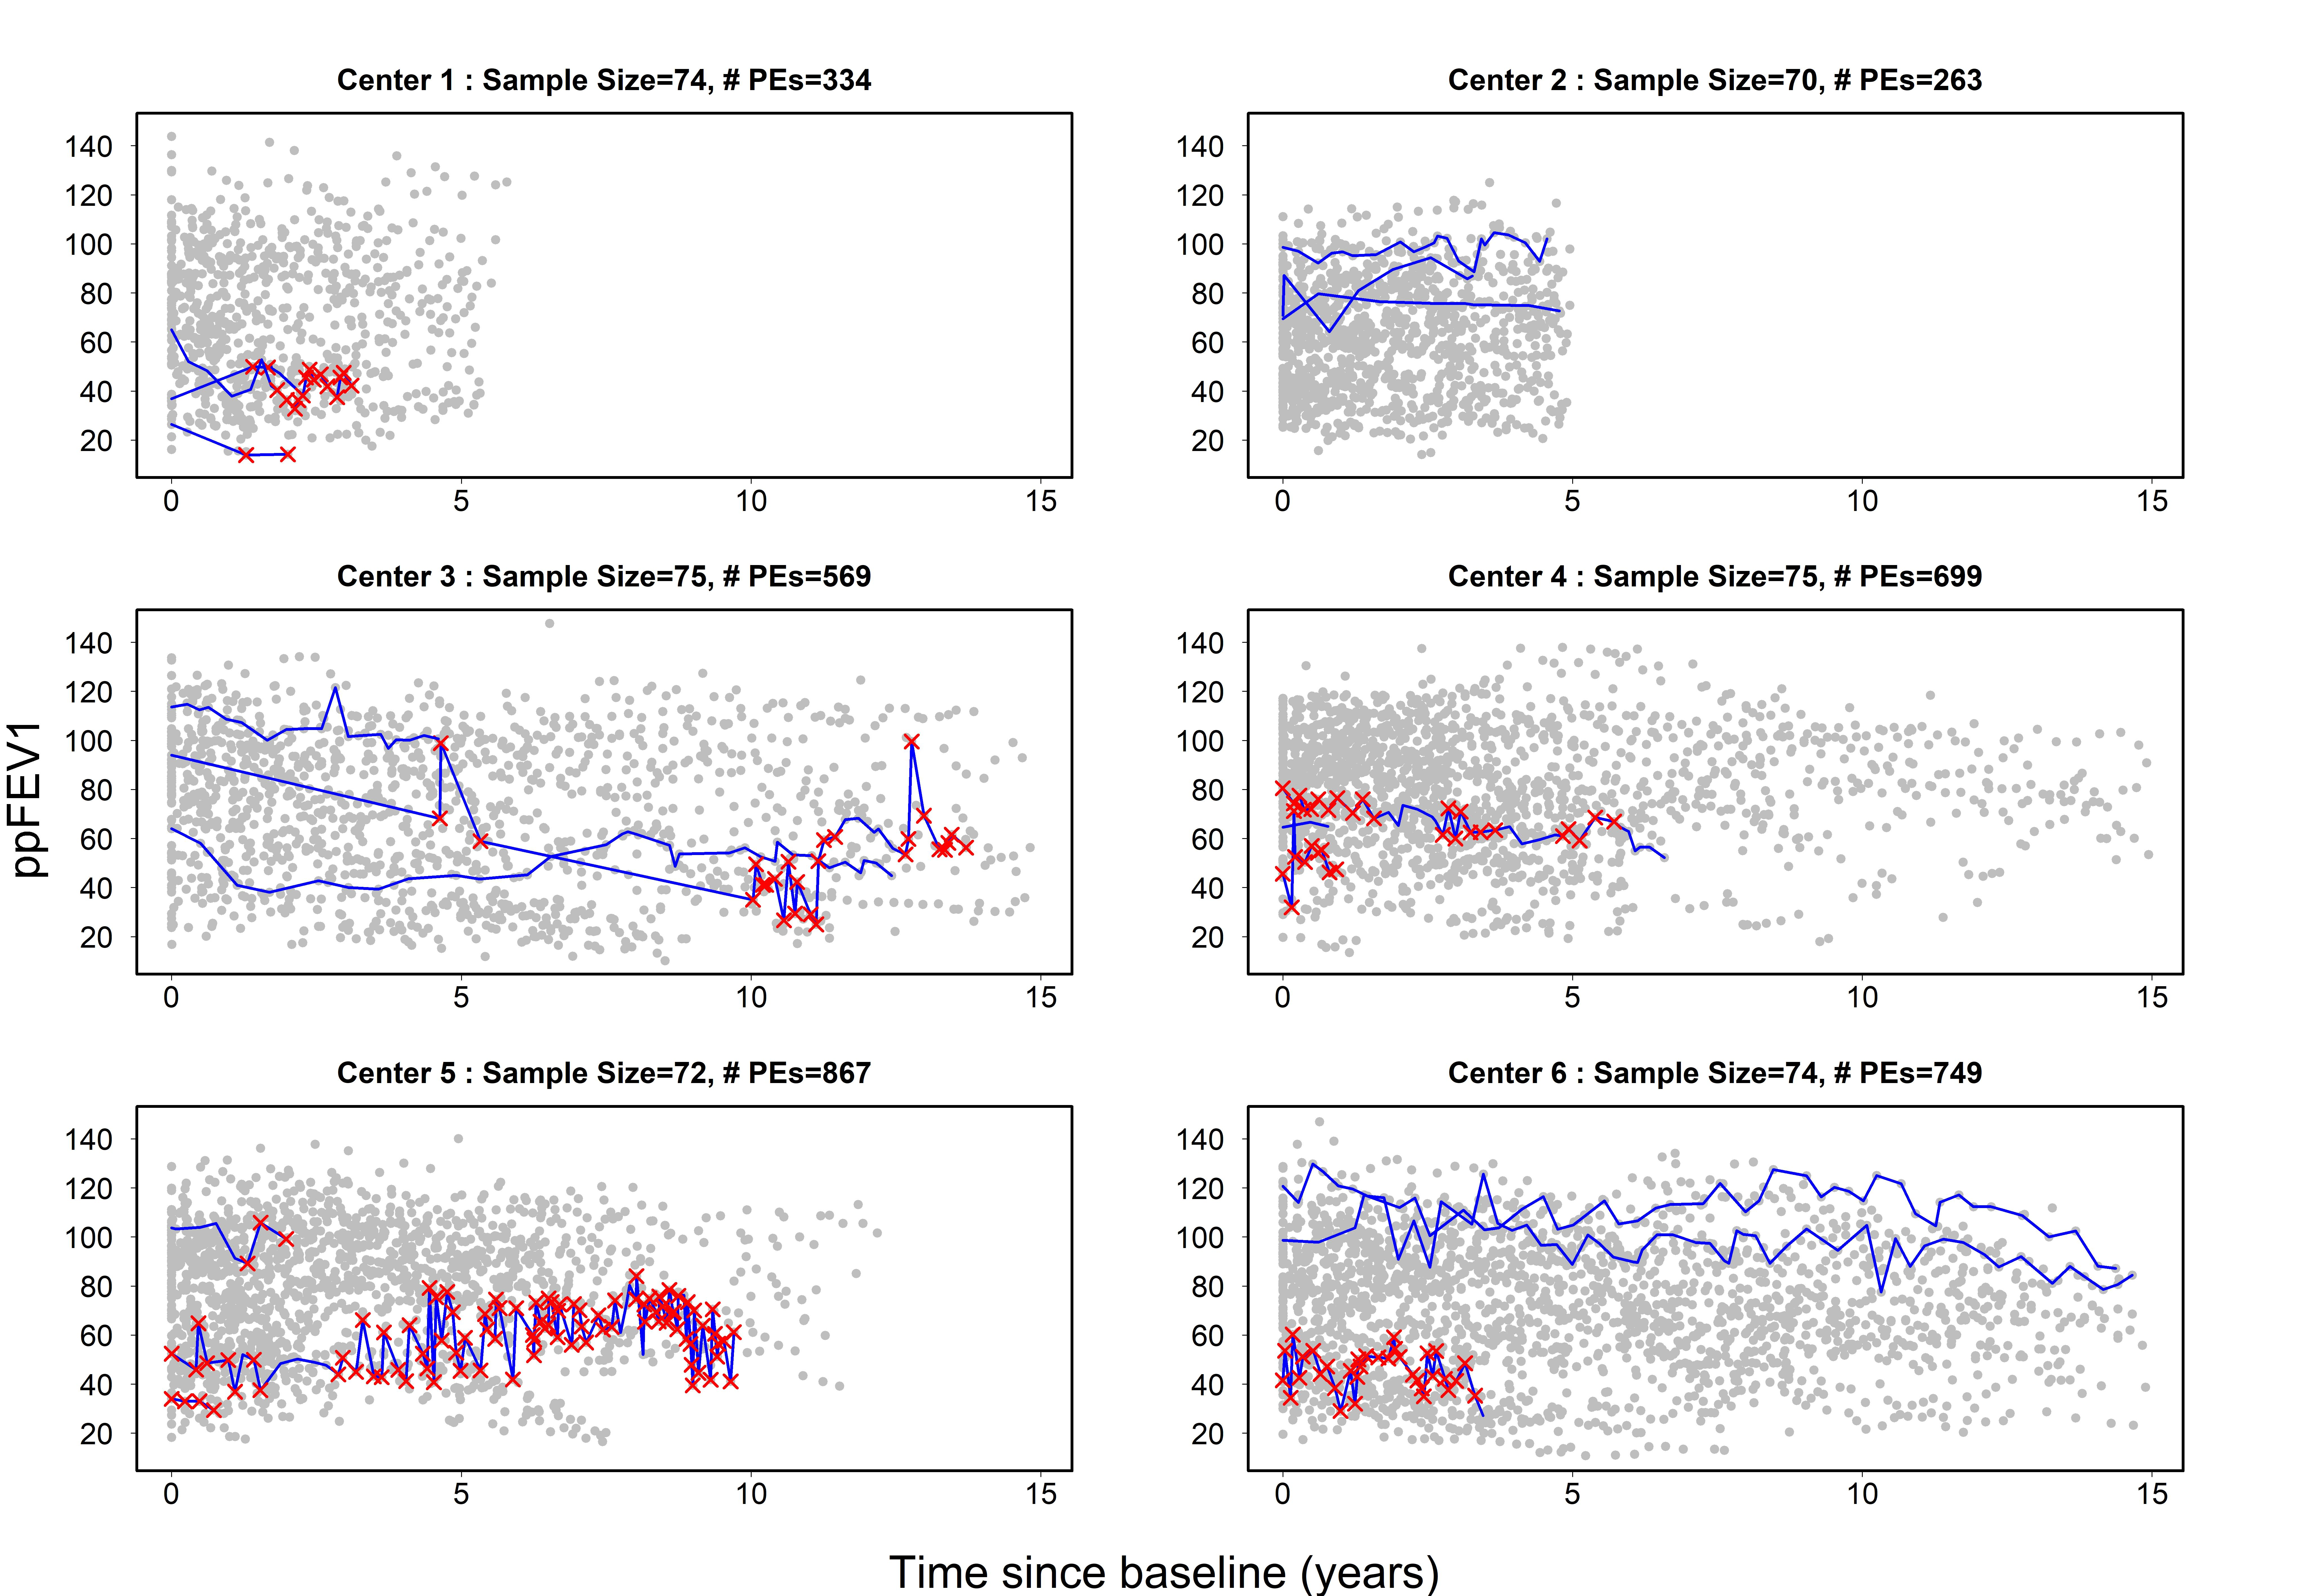
\includegraphics[width=\textwidth]{Figures/Chp3_trajectory.jpg}
\caption{Observed ppFEV1 against time since baseline (in years) for each center. Within each plot: three random specific profiles (solid blue line), observed values (gray dot) and recurrent PE events (red cross)}
\label{fig:chp3_traj}
\end{figure}

\subsection{Model Estimation}

For the sake of internal validation, we split our data into training and masking cohorts without loss of patients. For patients never experience PE event, we mask last period of their observations in terms of quantiles, while for rest of patients, we mask their last observed PE event. Analogously to the Chapter \ref{chp2}, we select predictors from aforementioned variables by \emph{Stepwise} method by a two-stage approach. To the end, we consider the following risk factors: i) For longitudinal submodel: baseline ppFEV1, time, quadratic of time, number of PEs within prior year, birth cohort, infection with pa and gender; ii) For event submodel: number of previous PEs, insurance use at baseline and gender. We examine a total of eight models (four joint models plus four two-stage models) and their comparisons with respect to LOOIC are represented in Table \ref{tab:chp3_comp}. Undoubtedly, all joint models are superior than corresponding two-stage models. From the statistical sight, the joint model with current value of ppFEV1 as the association structure in a calendar time scale outperforms others with the lowest LOOIC. Nonetheless, the choice between calendar time and gap time also depends on clinical interests and predictive performance. For illustration purpose, we pick the 'optimal' model from statistical perspective and its estimations with 90\% equal-tail credible intervals are summarized in Table \ref{tab:chp3_est} and convergence diagnosis plots are included in Appendix \ref{app:c}. From results of the longitudinal submodel, having higher ppFEV1 at entry corresponds to a higher ppFEV1 against time which reconciles with previous findings (\cite{TaylorRobinson2012}, \cite{Li2017}). The presence of infections with pa corresponds to worsen an average -1.15 (90\% CI [-1.64, -0.66]) units of ppFEV1. Being a male patient in older birth cohort is associated with higher ppFEV1. The variance component estimates indicate substantial heterogeneity within and between patients, in terms of large $\sigma,\sigma_{u0},\sigma_{u1}$. While less variations are found between centers given a frail $\sigma_b$. For the event submodel, we observe that males had 28.11\% ($exp(\gamma_3)-1$) lower risk to encounter PE compared to females. The usage of insurance at entry increased the risk by 33.64\% ($exp(\gamma_2)-1$), though it might not be statistically significant. One more count added to cumulative PE events is associated with a 1.01\% ($exp(\gamma_1)-1$) increase in the risk of current PE. Center-specific association parameters are all negative. Specifically, every one percentage predicted increase in 'true and unobserved' ppFEV1 would decrease 3.92\%, 4.88\%, 3.92\%, 3.92\%, 2.96\%, 3.92\% for the PE risk in Center 1 to Center 6, respectively. The non-zero center-specific Weibull shape parameters and frailty term are believed to facilitate the flexibility of the joint model for multi-center cohorts. 

\begin{table}[H]
  \small\sf\centering
   \captionsetup{justification=centering}
\caption{Model comparisons with the boldface as the smallest LOOIC}
\label{tab:chp3_comp}
 \begin{threeparttable}
\begin{tabular}{l|l|l|l|l}
\toprule
Association + Time scale & Model & $\mbox{LOOIC}$ \tnote{a} (SE\tnote{b} )  & $\mbox{LOOIC}_1$\tnote{c} (SE\tnote{b} ) & $\mbox{LOOIC}_2$\tnote{d} (SE\tnote{b} ) \\ \hline
\multirow{2}{*}{Slope + Gap} & Joint Model &  52551.9 (383.1) &	52490.3                                                 (231.5) &  61.6 (151.6) \\
                             & Two-stage Model & 52578.8 (385.7) &	52460.9 (232.3) & 117.9 (153.4)               \\ \hline
\multirow{2}{*}{Slope + Calendar} & Joint Model & 52563.0 (389.4) & 52473.1 (231.9) & 89.9 (157.5) \\
                                  & Two-stage Model & 52575.5 (390.2) & 52460.9 (232.3) & 114.6 (157.9) \\ \hline
\multirow{2}{*}{Value + Gap} & Joint Model & 52574.8 (383.4) & 52491.1 (230.6) & 83.7 (152.8)\\ 
                             & Two-stage Model & 52602.4 (384.5) & 52460.9 (232.3) & 141.5 (152.2)
                                            \\ \hline
\multirow{2}{*}{\textbf{Value + Calendar}} & \textbf{Joint Model} &                     \textbf{52537.3 (386.2)} &                                                            52486.4 (231.1) & 50.9 (155.1) \\ 
                                 & Two-stage Model & 52551.3 (388.3) &	52460.9 (232.3) & 90.4 (156)\\
\bottomrule
\end{tabular}
 \begin{tablenotes}[para]
    \footnotesize
        \item[a] Joint model; \item[b] Standard error approximated as byproduct of \emph{loo} package; \item[c] Longitudinal submodel; \item[d] Event submodel
    \end{tablenotes}
 \end{threeparttable}
\end{table}

\begin{table}[H]
  \small\sf\centering
  \captionsetup{justification=centering}
   \caption{Model estimations under Joint Model: Value+Calendar} \label{tab:chp3_est}
    \begin{threeparttable}
  \begin{tabular}{lcccccccc}
    \toprule
  & mean \tnote{1} & sd \tnote{2} & q5 \tnote{3} & q95 \tnote{3} & rhat \tnote{4} & ess\_bulk \tnote{5} & ess\_tail \tnote{6}\\
 \midrule
  \rowcolor{Gainsboro!60}
   \bf Longitudinal submodel &&&&&&& \\
    $\beta_0$ (intercept at age 6 years) & 7.59 & 1.59 & 5.09 &	10.15 &	1.00 & 713.45 & 1017.42 \\
    $\beta_1$ (baseline ppFEV1) & 0.86 & 0.02 &	0.83 & 0.89 & 1.00 &	553.14 & 1026.96\\
    $\beta_2$ (time since baseline) & -1.12	& 0.22 & -1.48 & -0.76 & 1.00 & 507.77 & 850.71\\
    $\beta_3$ ($\mbox{time since baseline}^2$) & -0.11 & 0.02 &	-0.14 &	-0.09 & 1.00 & 1049.14 & 1517.04\\
    $\beta_4$ (number of PEs within prior year) & -0.33 & 0.05 &	-0.4 & -0.25 & 1.00 & 1742.33 & 1373.07\\
    $\beta_5$ (birth cohort\tnote{$\ast$} $[1988, 1993)$) &3.17 &	1.15 & 1.28 & 5 & 1.00 &	592.67 & 961.08\\
    $\beta_6$ (birth cohort $[1993, 1998)$) & 3.48 & 1.22 &	1.32 & 5.46 & 1.00 & 503.65 &	885.29 \\
    $\beta_7$ (birth cohort $>$1998) & 4.57 & 1.24 & 2.49 &	6.69 & 1.00 &	474.94 & 805.76\\
    $\beta_8$ (pa) & -1.15 & 0.3 & -1.64 & -0.66 & 1.00 & 3771.81 &	1534.25\\
    $\beta_9$ (gender\tnote{$\ast$}  male)  & 1.59 &	0.83 & 0.23 & 2.93 & 1.01 &	470.46 & 924.86\\
    $\sigma$ (measurement error)& 9.07 & 0.08 & 8.94 & 9.2 & 1.00 & 2531.6 & 1556.46\\
    $\sigma_b$ (between centers, intercept) & 1.65 &	1.02 & 0.37 & 3.59 & 1.00 & 396.71 & 382.91\\
    $\sigma_{u0}$ (between patients, intercept) & 6.78 & 0.31 & 6.27 & 7.29 &	1.00 & 784.14 &	1288.57\\
    $\sigma_{u1}$ (between patients, slope)& 3.02 & 0.18 & 2.73 & 3.33 &	1.01 & 340 & 797.25\\
    $\rho$ (correlation, intercept and slope) & 0.18 &	0.07 & 0.06 & 0.3 &	1.01 & 193.5 & 482.79\\
     \rowcolor{Gainsboro!60}
  \bf Event submodel &&&&&&& \\
    $\gamma_0$ (intercept at age 6 years) & 2.02 & 0.28 & 1.57 & 2.5 & 1.00 &	246.96 & 484.67\\
    $\gamma_1$ (number of previous PEs) & 0.01 &	0 &	0 &	0.02 & 1.00 &	1991.24 & 1683.3\\
    $\gamma_2$ (baseline insurance use) & 0.29 & 0.19 &	-0.02 &	0.6 &	1.00 & 307.03 &	651.51\\
    $\gamma_3$ (gender\tnote{$\ast$}  male) & -0.33 & 0.19 & -0.64 & -0.02 & 1.00 &	265.64 & 564.24\\
    $\delta_1$(weibull shape, Center 1)  & 1.24 & 0.09 &	1.1 & 1.38 & 1.00 &	1975.36 & 1535.57\\
    $\delta_2$(weibull shape, Center 2)  & 1.01 & 0.08 &	0.88 & 1.13 & 1.00 & 2476.21 & 1642.13\\
    $\delta_3$(weibull shape, Center 3)  &1.28 &	0.07 & 1.16 & 1.4 &	1.00 & 754.97 &	1167.62\\
    $\delta_4$(weibull shape, Center 4)  & 1.26 & 0.06 &	1.16 & 1.36 & 1.00 & 1780.2 & 1785.08\\
    $\delta_5$(weibull shape, Center 5)  & 1.24 & 0.06 &	1.15 & 1.34 & 1.00 & 1466.17 & 1421.63\\
    $\delta_6$(weibull shape, Center 6)  & 1.07 & 0.05 &	0.98 & 1.15 & 1.00 & 1152.13 & 929.47\\
    $\sigma_v$(between patients, frailty)  & 1.6 &	0.1 & 1.44 & 1.77 &	1.00 & 527.68 &	762.6\\
     \rowcolor{Gainsboro!60}
 \bf Association &&&&&&& \\
    $\alpha_1$ (submodel link, Center 1) & -0.04 & 0 & -0.05 & -0.03 & 1.01 &	455.98 & 786.05\\
    $\alpha_2$ (submodel link, Center 2) & -0.05 & 0.01 &	-0.06 &	-0.04 &	1.00 & 331.54 &	639.72\\
    $\alpha_3$ (submodel link, Center 3) & -0.04 & 0 & -0.05 & -0.04 & 1.00 &	455.63 & 797.91\\
    $\alpha_4$ (submodel link, Center 4) & -0.04 & 0 & -0.04 & -0.03 & 1.01 &	359.67 & 666.75\\
    $\alpha_5$ (submodel link, Center 5) & -0.03 & 0 & -0.03 & -0.02 & 1.01 &	323.03 & 590.15\\
    $\alpha_6$ (submodel link, Center 6) & -0.04 & 0 & -0.05 & -0.04 & 1.01 &	381.33 & 895.84\\
    \bottomrule
  \end{tabular}
 \begin{tablenotes}[para]
    \footnotesize
    \item[1] posterior mean; \item[2] Monte Carlo standard deviation; \item[3] posterior quantiles at 5\% and 95\%; \item[4] potential scale reduction factor (at convergence, rhat=1) \item[5] bulk effective sample size; \item[6] tail effective sample size; \item[$\ast$] Reference: Birth cohort $<1988$; Gender female
    \end{tablenotes}
    \end{threeparttable}
\end {table}

\subsection{Model Diagnostics}

In this section, we validate the assumptions of our joint model (Value+Calendar) through basic residual tools by following the methodology addressed in \cite{Rizopoulos2012d}. For the longitudinal submodel, we implement conditional standardized residuals to check the assumptions of homoscedasticity and normality (see Plot A in Figure \ref{fig:chp3_diag}). We observe that there is no systematic trend from the fitted loess curve, despite some heavy-tailed issues (see Plot B in Figure \ref{fig:chp3_diag}). For the event submodel, we investigate the martingale residuals based on the counting process. Subject-specific martingale residual at time $t$ can be viewed as the difference between the observed number of events by $t$, and the expected number of events by the same time. The fitted zero loess curve illustrates the reasonable performance of the event submodel, despite some outliers. Another diagnostic method, which is called Cox-Snell residuals (\cite{Cox1968}), can be utilized to compare the observed distribution of cumulative hazard with the expected one unit exponential distribution. Cox-Snell residuals are reserved for the time-to-event case, hence we estimate the subject-specific cumulative hazard for the first PE event. Kaplan-Meier estimate (\cite{Kaplan1958}) of the survival function of the censored Cox-Snell residuals is illustrated in Plot D in Figure \ref{fig:chp3_diag}. We observe acceptable discrepancies between the fit of Kaplan-Meier estimate and the expected asymptotic distribution. Apart from previous Gauss-Kronrod approach, here we evaluate the numerical integrand via \emph{integrate} function of R package \emph{stats} (v4.0.2, \cite{R2020}).     

\begin{figure}[H]
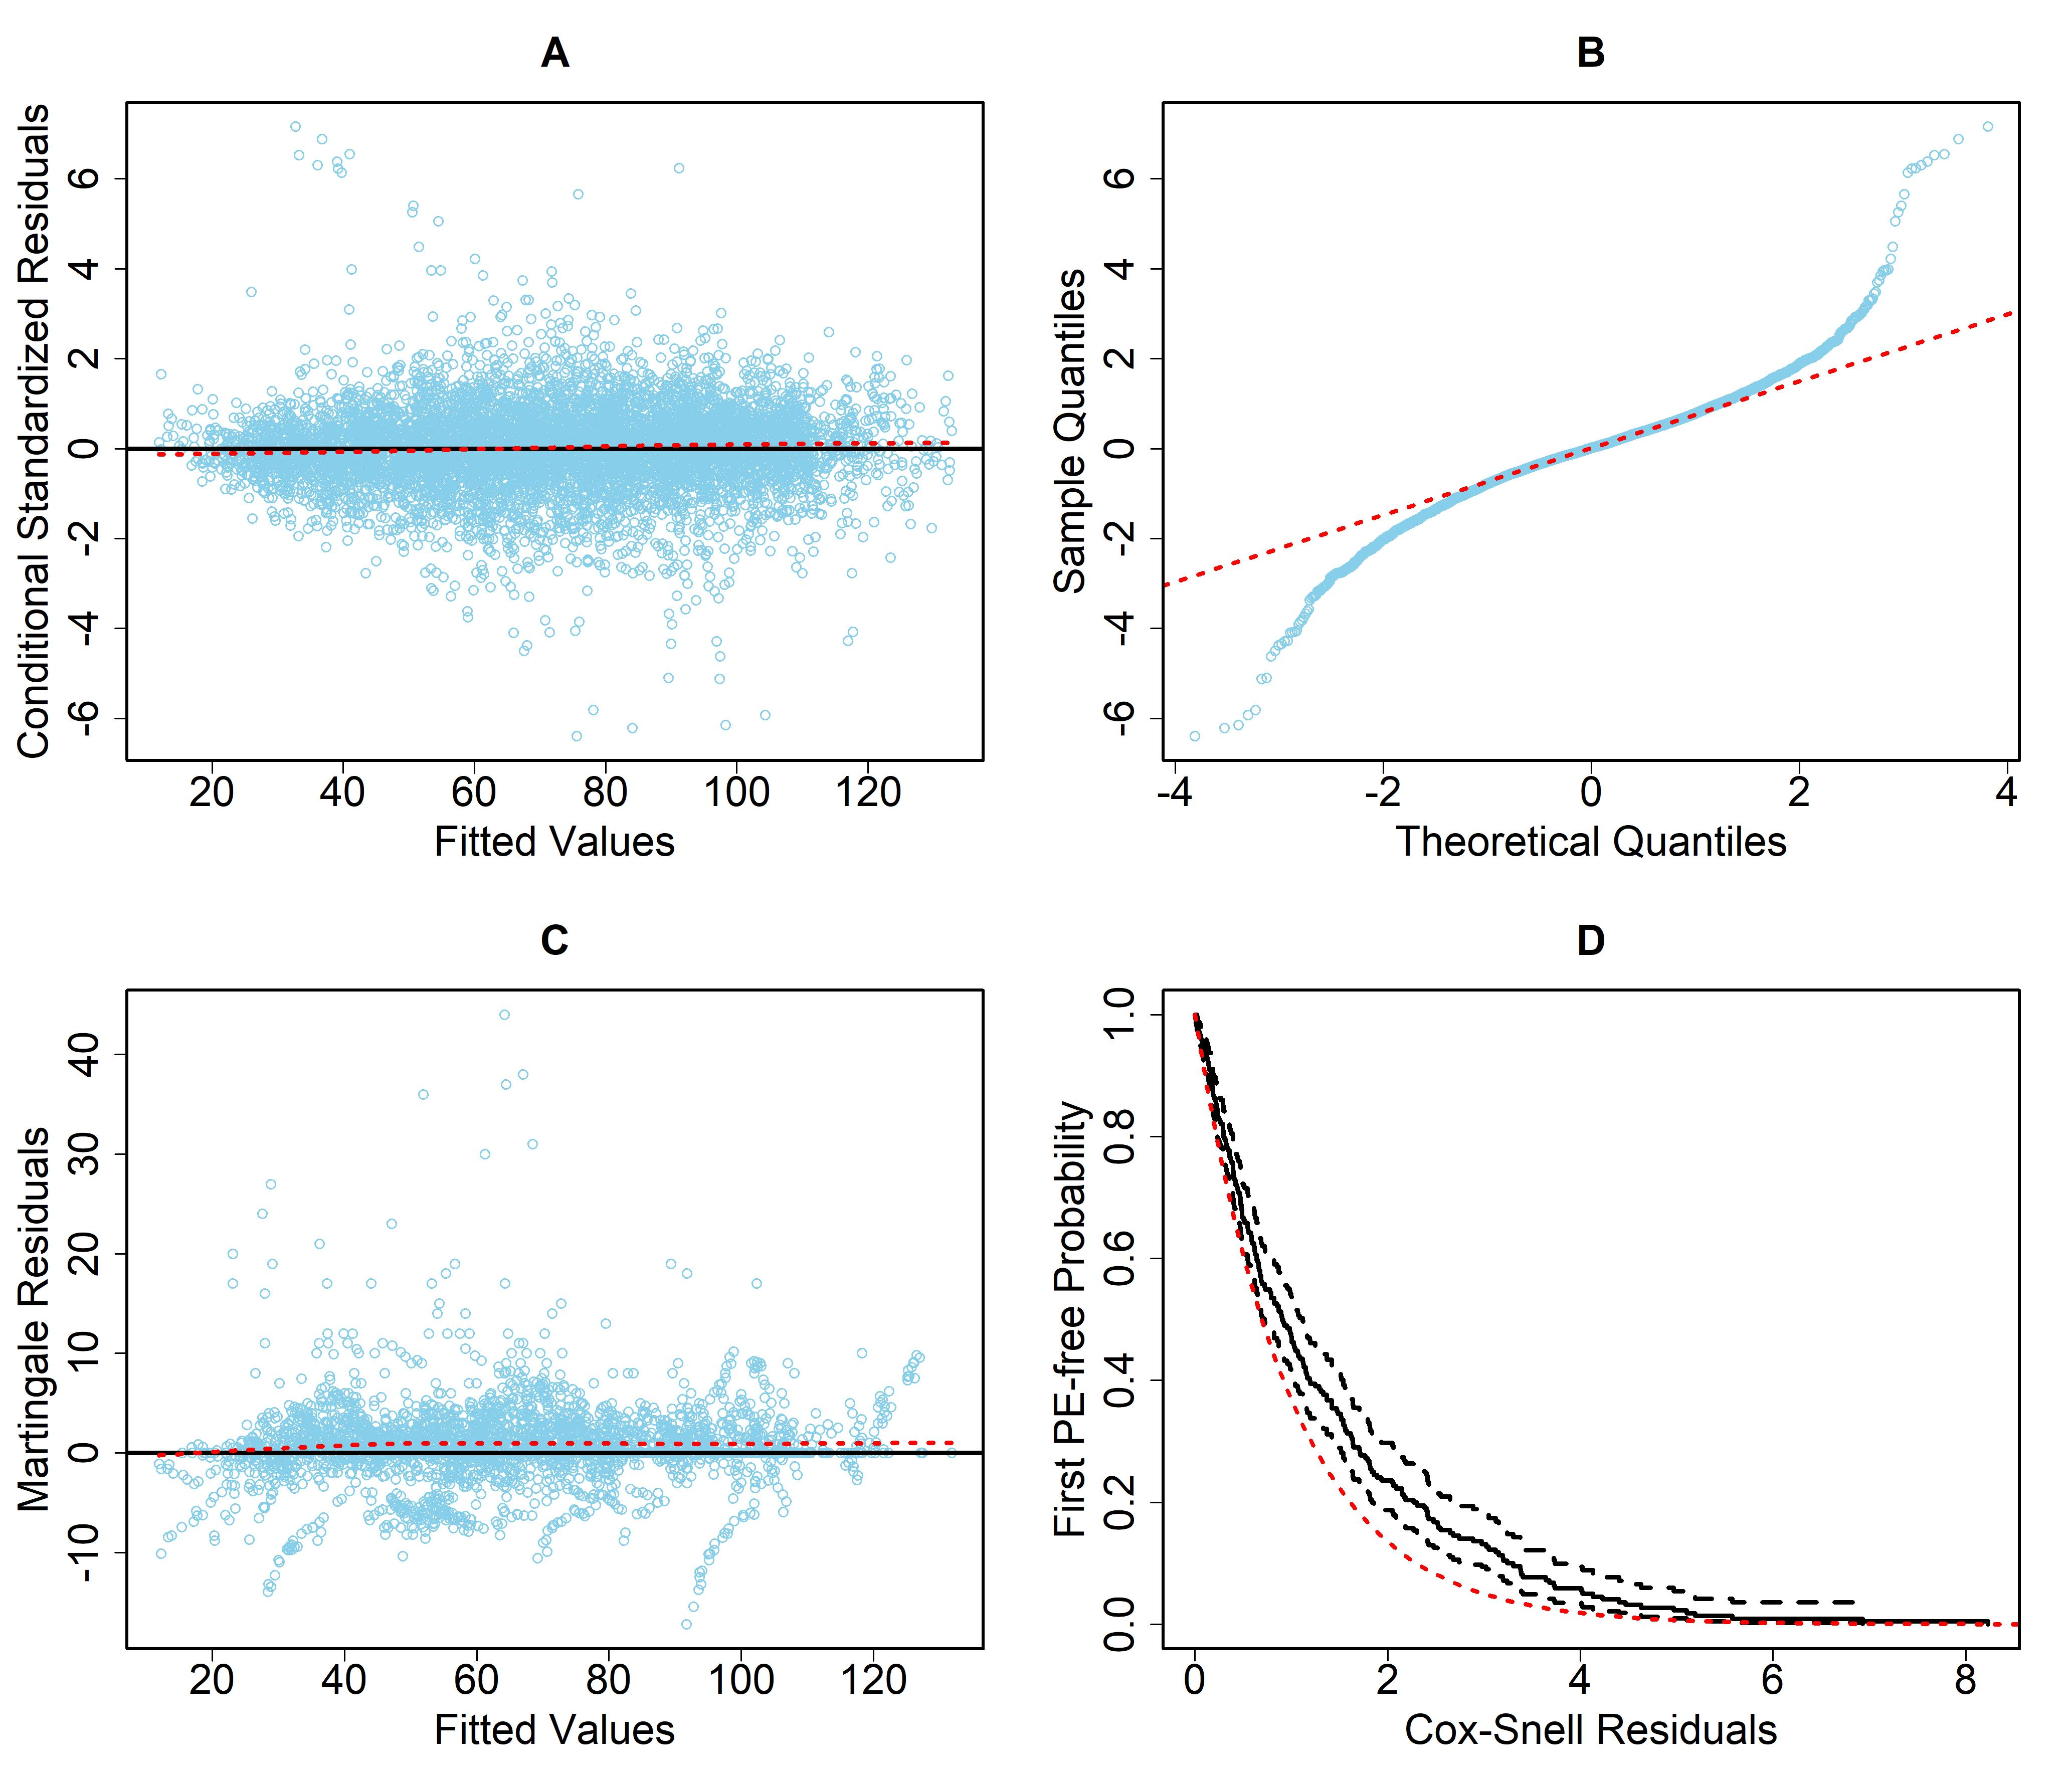
\includegraphics[width=0.9\textwidth]{Figures/Chp3_DIAG.jpg}
\caption{Residuals diagnostic plot for the proposed joint model. Upper panel: subject-specific standardized residuals versus fitted values (A) and normal Q-Q plot for longitudinal submodel (B). Lower panel: subject-specific martingale residuals versus fitted values (C) and Cox-Snell residuals for event submodel (D). Red dashed lines in A \& C are fitted loess curve; that in B \& D are normal curve and exponential curve, respectively}
\label{fig:chp3_diag}
\end{figure}

\subsection{Predictive Performance}

To assess predictive performance of proposed joint models, we compute time-dependent AUC and MPE for each joint model under various future time scenarios and results are shown in Table \ref{tab:myauc}. Unlike the conventional method used in \cite{Ren2021}, that is to assign a common prediction start time ($t$), we characterize individual prediction time ($t_{li}$) from the end time of each patient's last available encounter. The future times ($t'$) are summarized by the quartile of their stop times and the concept of patients at risk denotes that patients have not yet experienced the next occurrence of PE at $t'$.  

All joint models represent the excellent discriminate and calibrate capability in the longer term run. Figure \ref{fig:chp3_pred} forecast random patients who are still at risk after their last observed measurements under the joint model Value+Calendar. We note that Patient 202 and Patient 284 represent two extreme cases, suggesting that higher lung function reduces the risk of the next PE event, while the latter patient needs a timely care and prevention given high risk for the next PE event. From virtual inspection, we observe that averaged ppFEV1 value and frequency of previous PE occurrences are not ignorable risk factors for the prognostic probability of the next PE event.

\begin{table}[H]
  \small\sf\centering
  \captionsetup{justification=centering}
\caption{Predictive performance of proposed joint models}
\label{tab:myauc}
\begin{threeparttable}
\begin{tabular}{c|c|l|c|c}
\toprule
\textbf{Future time (years)} & \textbf{Num Patients at risk} & \textbf{Joint Model} & \textbf{AUC} & \textbf{MPE} \\ \hline
\multirow{4}{*}{2.73} & \multirow{4}{*}{118} & Slope + Gap & 0.61 &	0.28 \\
                      &                      & Slope + Calendar & 0.64 & 0.27 \\
                      &                      & Value + Gap & 0.66 & 0.27 \\
                      &                      & Value + Calendar & 0.68 & 0.26 \\ \cline{1-5}
\multirow{4}{*}{5.10} & \multirow{4}{*}{141} & Slope + Gap &	0.89 & 0.14 \\
                     &                      & Slope + Calendar & 0.88 & 0.14 \\
                     &                      & Value + Gap & 0.90 & 0.14 \\
                     &                      & Value + Calendar & 0.88 &	0.14\\ \cline{1-5}
\multirow{4}{*}{7.84} & \multirow{4}{*}{107} & Slope + Gap & 0.92 &	0.12 \\
                      &                      & Slope + Calendar & 0.91 & 0.13 \\
                      &                      & Value + Gap & 0.92 &	0.12 \\
                      &                      & Value + Calendar & 0.92 & 0.13\\ 
\bottomrule
\end{tabular}
\begin{tablenotes}[para]
\footnotesize
Abbreviation: AUC=area under curve; MPE=mean predictive error
\end{tablenotes}
\end{threeparttable}
\end{table}

\begin{figure}[ht]
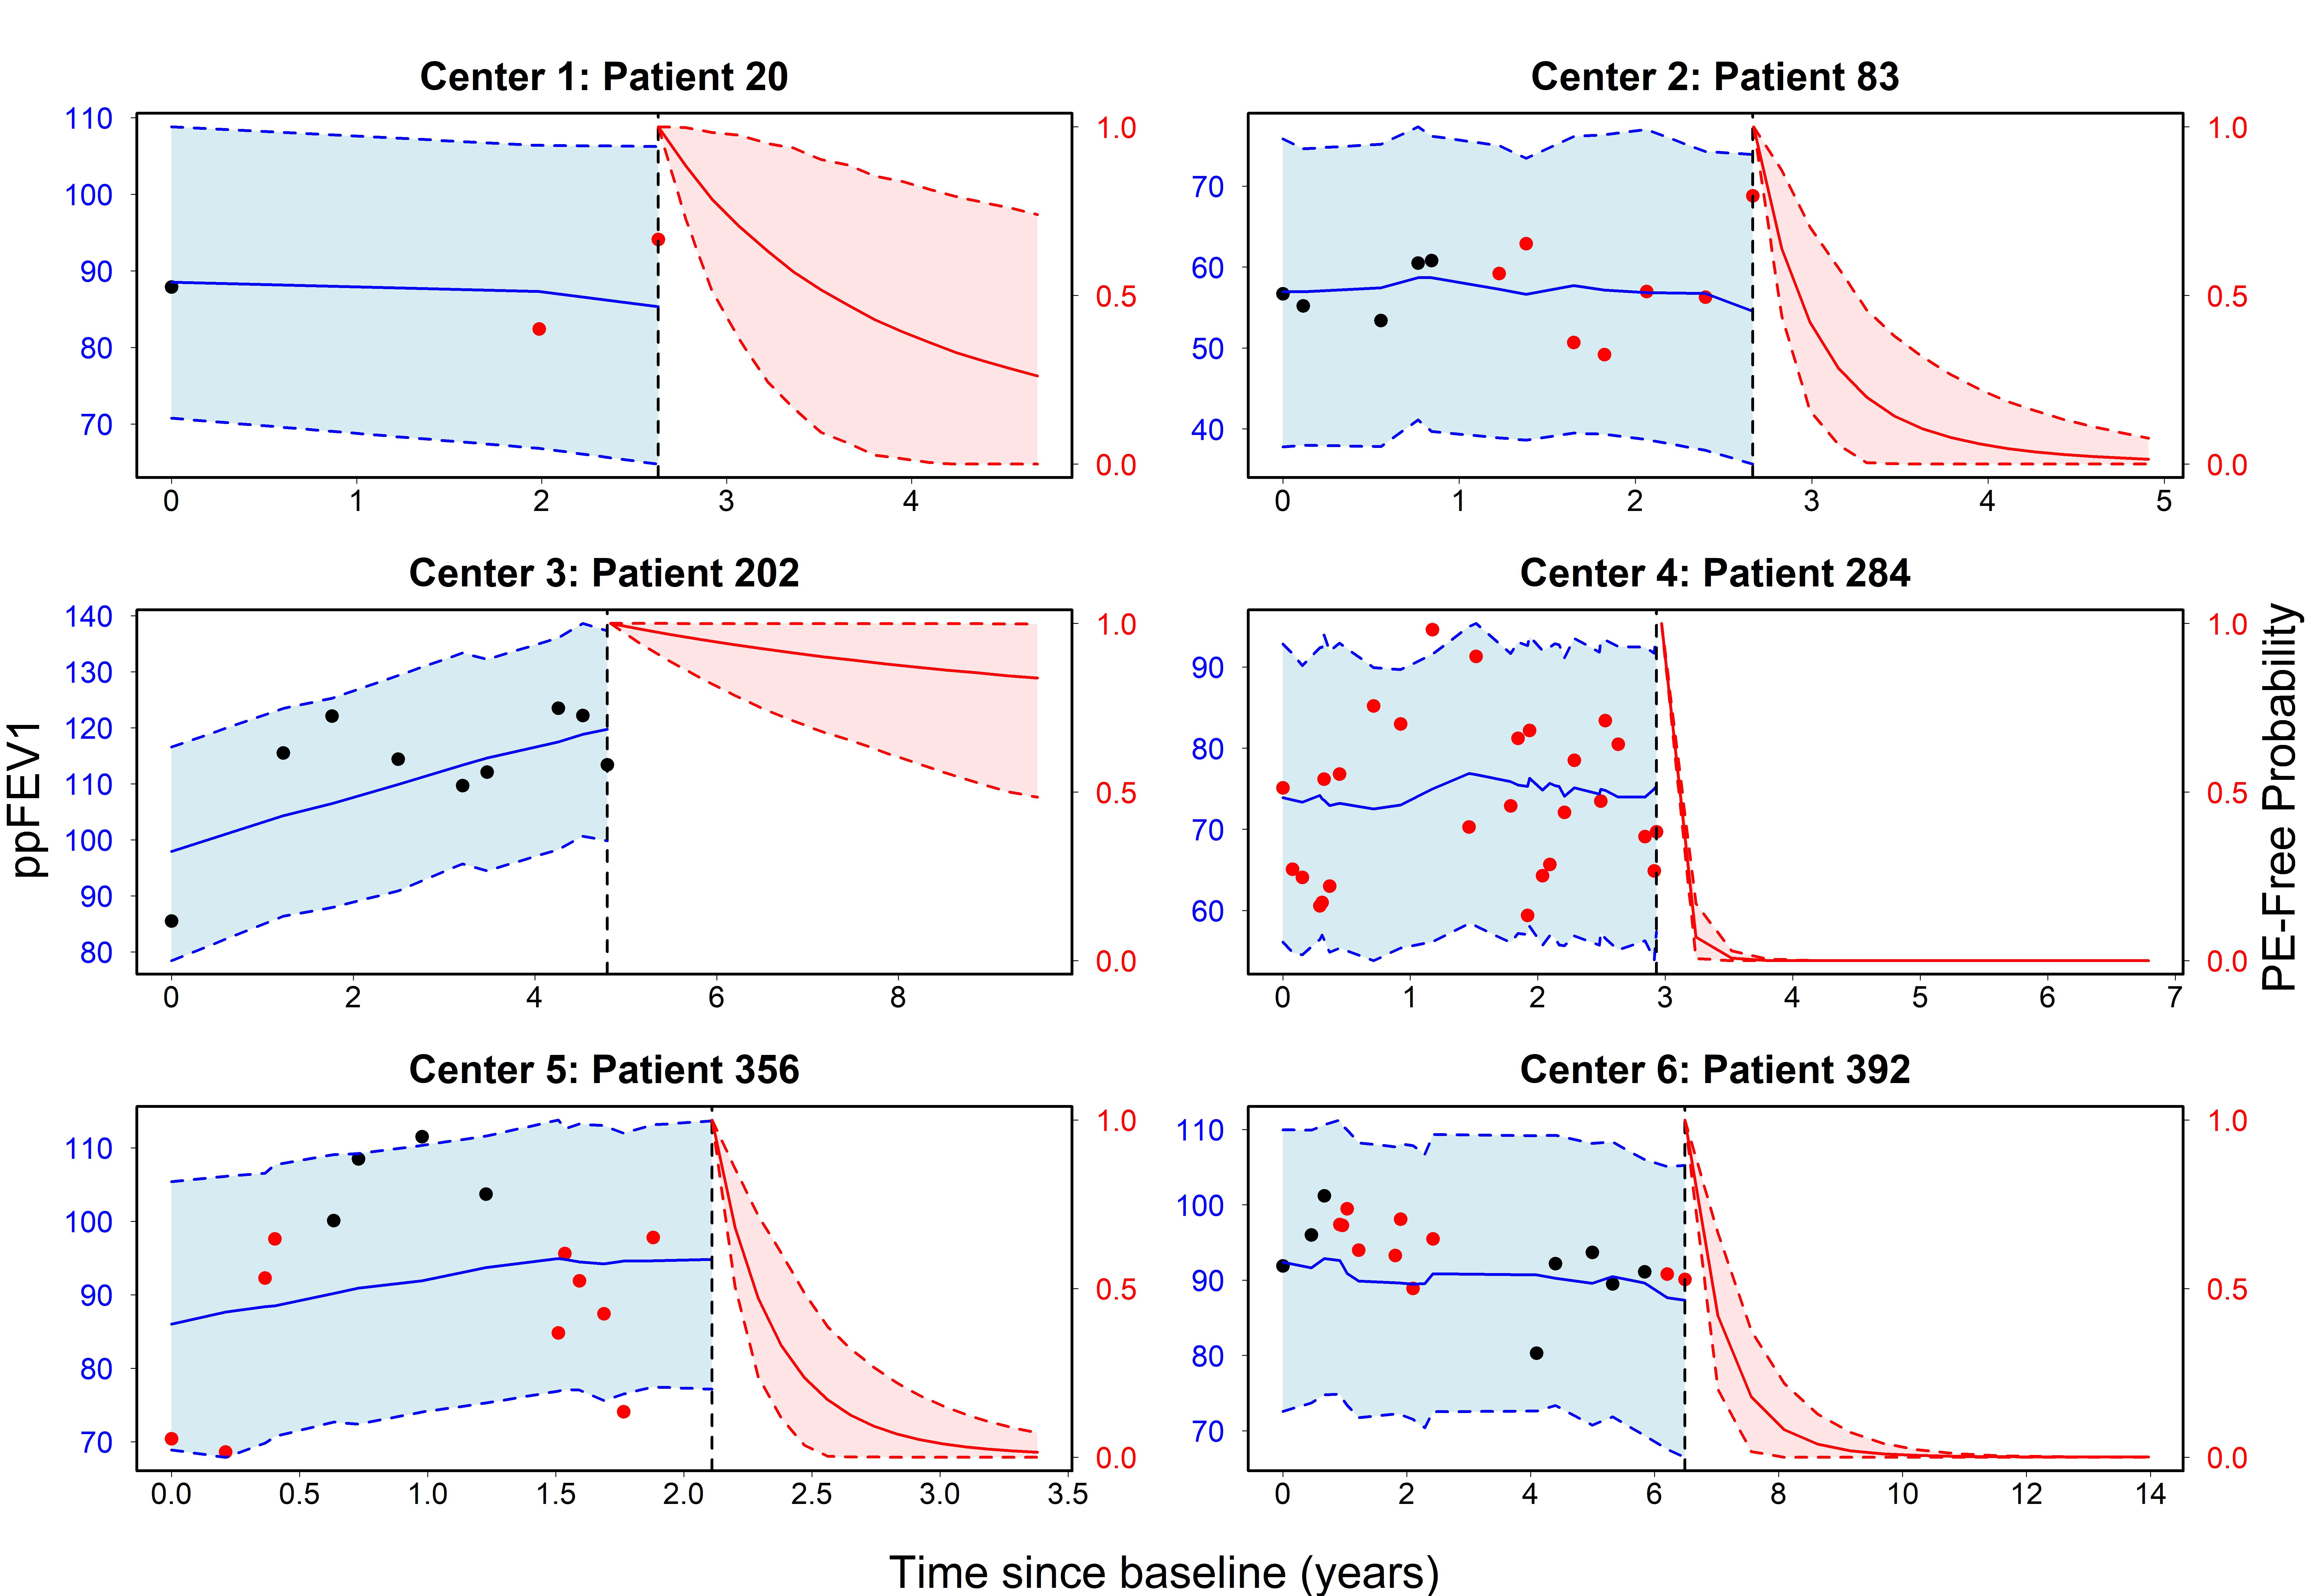
\includegraphics[width=\textwidth]{Figures/Chp3_PRED_PLOT2.jpg}
\caption{Individual predictions against time by centers, including observed ppFEV1 (dots) illustrated by PE event (red dots) and non-PE event (black dots), fitted value of ppFEV1 (blue lines), prognostic PE-free probability (red lines) and 95\% credible intervals (bands)}
\label{fig:chp3_pred}
\end{figure}

\section{Discussion} \label{sec:chp3_diss}

In this chapter, we have proposed a multilevel Bayesian joint model for a monitoring CF data depicted by hierarchical structures and irregularly clinical visits. Our novel model allows for center-specific association parameters to quantify the strength of the correlation between the two processes and such approach facilitate individual prognosis towards personalized medical monitoring. Furthermore, we provide detailed simulation algorithm and \emph{Stan} codes by extending the work of \cite{Brilleman2018}. Despite the large cost of computing time due to large sample size and approximation using Gauss-Kronrod quadrature rule, Bayesian methodology provides convincing benefits, especially lead to posterior predictive distributions and release the numerical integral burden through Monte Carlo samplings.

The availability of robust software packages is limited. In Chapter \ref{chp1}, we have introduced briefly R packages \emph{JMBayes2} and \emph{rstanarm}. There also exists R package frailtypack (\cite{Rondeau2019}), which allows for joint nested frailty models in the context of the joint modeling for recurrent events with terminal event, for hierarchically clustered data. Notwithstanding that it closely relates to our topic, it adapts maximum penalized likelihood estimation rather than the Bayesian approach. For this sake, we implement our own R code with \emph{Stan} programs via \emph{CmdStanR} interface to Stan (\cite{Gabry2022}). To enhance rigor and reproducibility of our proposed model, the example codes have been posted in Appendix \ref{app:c}.  

This article would be considered in the light of some limitations and interesting extensions. We limit our work on recurrent events without presence of terminal event. However, it may be necessary to include additional submodel for a terminal event in the context of an extended joint model in the future research. Notwithstanding we present the individual prognostic rationale for in-sample patients, there exists great practical and theoretical interest to investigate out-of-sample predictions in terms of dynamic feature, which was proposed with novelty for univariate joint model in \cite{Proust-Lima2009} and \cite{Rizopoulos2011}; applied for joint model with recurrent events in \cite{Ren2021} or joint model for recurrent events with a terminal event in \cite{Mauguen2013}. Furthermore, with respect to the specific forecast period, it might be interesting to access the predictive performance at several clinical relevant window widths (e.g., age 18 to 23 or age 25 to 30), which are dependent on frequencies of (next) PE events. Though predictive probability of next event is welcome, an alternative measure is mean residual life (MRL), which provides the expected time to the next event occurrence (\cite{Deep2020}). The advantage of MRL lies in its clinical interpretation between physicians and patients. We utilize ubiquitous random intercept-slope model for the longitudinal submodel, while it can be replaced by some other novel Gaussian process models, nevertheless, the complexity is unlikely to be warranted. In this paper, we barely include time-varying covariates for the event submodel, hence, more time-dependent risk factors could be further investigated. With respect to various baseline hazard function candidates, alternatives such as bsplines, piecewise-constant are undergoing. Lastly, we investigate the routine diagnostics of joint model, which has not received much attention in the joint modeling literature. Readers who are interested in a thorough discussion about this topic can refer to \cite{Rizopoulos2012d} for some new insights. 


\chapter{Conclusion and Future Work}\label{chp4}

To summarize, we have proposed novel multilevel Bayesian joint models for personalized prediction of PE risk in hierarchically structured CF data. The joint model is in the sense of joint analysis of two types of outcomes simultaneously, which including ppFEV1 as a biomarker and PE as a binary event. Specifically, we account for PE in two submodel frameworks: i) GLMM; ii) survival model. In the context of GLMM, we demonstrate that the center with more severe CF patients tends to have higher risk of PE and patients with worse averaged lung function are more likely to experience PE. Whilst with respect to survival model, every one percentage predicted increase in 'true and unobserved' ppFEV1 would decrease 3.92\%, 4.88\%, 3.92\%, 3.92\%, 2.96\%, 3.92\% for the PE risk from selected Center 1 to Center 6. The novelty of this dissertation is evident, such as center-specific power parameter, center-specific parameter for the association structure and baseline hazard function, individual-specific prediction start time and customized applicable Stan programs.

In both chapters, we have implemented 80-20\% cross-validation. However, a recently published paper proposed sample size guidelines for developing a clinical prediction model \cite{Riley2020}. The article recommended resampling methods (such as bootstrapping) as the internal validation with at least 10 events for each predictor parameter. Another potential issue with our employed \emph{Stepwise} algorithm has been raised in a recent paper by \cite{Harhay2020}. They suggested that such procedure might lead to bias and overfitting problems. The backwards variable selection algorithm with a large significant level seems to be a better approach (\cite{Heinze2017}). From the clinical perspective in our application context, \emph{Stepwise} approach provides a straightforward means of feature selection, and from the statistical point of view, predictors have minimal impacts on predictive performance as long as the covariance structure is well specified. The past and current work highlight the need to proceed carefully about intended purpose of the prediction model while prioritizing feature selection elements as appropriate.  

Additional sources of bias might be brought by left-truncation within CF registry data. Although we remedy it by adding birth cohort as a covariate, this topic might be of interest to be devised by referring to \cite{Krol2016} and \cite{Piccorelli2012}. Given the fact that joint model comes at a cost of intensive computational time, as suggested in \cite{Barrett2019}, a possible modeling strategy can be to use the two-stage method for model selection and the joint model for inference. Moreover, an embarrassing parallel-MCMC algorithm mentioned in \cite{Ren2021} might be helpful to reduce running time. Finally, the RShiny app (\cite{shiny2013}) is under programming with the aim to facilitate the individual (dynamic) prediction from our proposed joint models.  

 % There are many widely applied R packages for GLMM, namely, lme4 by Bates et al. (2015), MCMCglmm by Hadfield 2010, brms by Burkner (xx), GLMMadaptive by Rizopoulos xx. Among which brms is for Bayesian GLMM using Stan. Though these packages more or less support variable existing link functions, our customized link function is not yet incorporated. Therefore, we code by ourselves via user friendly interfact rstan.  


% \include{chap5}

\bibliographystyle{spbasic}
\begin{SingleSpace}
\bibliography{reference}
\end{SingleSpace}

\appendix
\chapter{Appendix for Chapter \ref{chp1}} \label{app:a}
\section{Data}

\begin{minted}{R}
# eight\_schools.data.R
J <- 8
y <- c(28, 8, -3, 7, -1, 1, 18, 12)
sigma <- c(15, 10, 16, 11, 9, 11, 10, 18)
\end{minted}

\section{Stan program}
\begin{minted}{R}
# eight_schools_cp.stan

data {
  int<lower=0> J;
  real y[J];
  real<lower=0> sigma[J];
}

parameters {
  real mu;
  real<lower=0> tau;
  real theta[J];
}

model {
  mu ~ normal(0, 5);
  tau ~ cauchy(0, 5);
  theta ~ normal(mu, tau);
  y ~ normal(theta, sigma);
}

# eight_schools_ncp.stan

data {
  int<lower=0> J;
  real y[J];
  real<lower=0> sigma[J];
}

parameters {
  real mu;
  real<lower=0> tau;
  real theta_tilde[J];
}

transformed parameters{
  real theta[J];
  for (j in 1:J)
    theta[j]=mu+tau*theta_tilde[j];
}

model {
  mu ~ normal(0, 5);
  tau ~ cauchy(0, 5);
  theta_tilde ~ normal(0, 1);
  y ~ normal(theta, sigma);
}

\end{minted}

\section{R code}

\begin{minted}{R}
# Setup

library(gridExtra) #v2.3
library(bayesplot) #v1.8.1
library(dplyr) #v1.0.5
library(cmdstanr) #v0.4.0
library(rstan) #v2.21.1
options(mc.cores = parallel::detectCores())
rstan_options(auto_write = TRUE)
input_data <- read_rdump('eight_schools.data.R')

# Fit

##Default: adapt_delta=0.8, max_treedepth=10, iter=2000, warmup=1000
###rstan
    fit_cp <- rstan::stan('eight_schools_cp.stan', data = input_data,
                   iter = 2000, warmup = 1000, chains = 2, seed = 2022)
                   
    rstan::get_elapsed_time(fit_cp)
    
    fit_ncp <- rstan::stan(file = 'eight_schools_ncp.stan', data = input_data,
                   iter = 2000, warmup = 1000, chains = 2, seed = 2022)

###cmdstanr
  mod.cp <- cmdstanr::cmdstan_model('eight_schools_cp.stan')
  fit_cp_cmd <- mod.cp$sample(data = input_data, chains = 2,
                save_warmup = FALSE, parallel_chains = 2, refresh = 500, seed=2022)

  mod.ncp <- cmdstanr::cmdstan_model('eight_schools_ncp.stan')
  fit_ncp_cmd <- mod.ncp$sample(data = input_data, chains = 2,
                save_warmup = FALSE, parallel_chains = 2, refresh = 500,
                seed=2022)

# Results
##rstan
tau_cp0 <- as.data.frame(extract(fit_cp, par='tau', permuted=TRUE))
tau_cp <- tau_cp0 %>% 
          rename(tau.cp=tau) %>% 
          mutate(log.tau.cp=log(tau.cp))

tau_ncp0 <- as.data.frame(extract(fit_ncp, par='tau', permuted=TRUE))
tau_ncp <- tau_ncp0 %>% 
           rename(tau.ncp=tau) %>% 
           mutate(log.tau.ncp=log(tau.ncp))

tau_all <- cbind(tau_cp,tau_ncp) %>% 
            mutate(iter=1:2000,
                 chain=rep(1:2,each=1000))

tau_all$mean.cp <- sapply(tau_all$iter, function(n) mean(tau_all$log.tau.cp[1:n]))
tau_all$mean.ncp <- sapply(tau_all$iter, function(n) mean(tau_all$log.tau.ncp[1:n]))

tau_all$div.cp <- c(get_sampler_params(fit_cp, inc_warmup=FALSE)[[1]][,'divergent__'],
                   get_sampler_params(fit_cp, inc_warmup=FALSE)[[2]][,'divergent__'])

tau_all$div.ncp <- c(get_sampler_params(fit_ncp, inc_warmup=FALSE)[[1]][,'divergent__'],
                    get_sampler_params(fit_ncp, inc_warmup=FALSE)[[2]][,'divergent__'])
##cmdstanr
tau_cp_cmd <- fit_cp_cmd$draws('tau',format='df') %>% 
              rename(chain=.chain,
                     tau.cp=tau) %>% 
              mutate(log.tau.cp=log(tau.cp),
                     iter=1:2000)

tau_ncp_cmd <- fit_ncp_cmd$draws('tau',format='df') %>% 
                rename(chain=.chain,
                       tau.ncp=tau) %>% 
                mutate(log.tau.ncp=log(tau.ncp),
                       iter=1:2000)

tau_all_cmd <- tau_cp_cmd %>% 
              left_join(tau_ncp_cmd, by=c('chain','iter','.draw'))


mean.cp <- sapply(tau_all_cmd$iter, function(n) mean(tau_all_cmd$log.tau.cp[1:n]))
tau_all_cmd$mean.cp <- mean.cp

mean.ncp <- sapply(tau_all_cmd$iter,function(n) mean(tau_all_cmd$log.tau.ncp[1:n]))
tau_all_cmd$mean.ncp <-mean.ncp

diag.cp <- fit_cp_cmd$sampler_diagnostics(format = "df")
diag.ncp <- fit_ncp_cmd$sampler_diagnostics(format = "df")

tau_all_cmd$div.cp <- diag.cp$divergent__
tau_all_cmd$div.ncp <- diag.ncp$divergent__

sum(tau_all$div.cp)/2000 #0.0115
sum(tau_all$div.ncp)/2000 #0
sum(tau_all_cmd$div.cp)/2000 #0.04
sum(tau_all_cmd$div.ncp)/2000 # 0

#Plot
light.orange='#E69F00'
orange='#D55E00'
light.blue='#56B4E9'
blue='#0072B2'

#Figure 1.1
{
  jpeg("Chp1_mean_tau.jpg", width = 350, height = 300, units='mm', res = 300)
  par(cex.lab=2, cex.axis=1.5)
  par(mar = c(4, 5, 0.5, 0.5))
  plot(NA, xlim=c(1,2000), ylim=c(0, 2),xlab="Iteration", ylab="mean of log(tau)")
  points(tau_all$iter,tau_all$mean.cp,col=light.orange, pch=16,cex=2)
  points(tau_all$iter,tau_all$mean.ncp,col=orange, pch=16,cex=2)
  points(tau_all_cmd$iter,tau_all_cmd$mean.cp,col=light.blue, pch=16,cex=2)
  points(tau_all_cmd$iter,tau_all_cmd$mean.ncp,col=blue, pch=16,cex=2)
  abline(h=0.7657852, col='#009E73', lty="dashed", lwd=5)
  
  div_iter_cp <- tau_all$iter[which(tau_all$div.cp==1)]
  div_mean_cp <- tau_all$mean.cp[which(tau_all$div.cp==1)]
  div_iter_cp_cmd <- tau_all_cmd$iter[which(tau_all_cmd$div.cp==1)]
  div_mean_cp_cmd <- tau_all_cmd$mean.cp[which(tau_all_cmd$div.cp==1)]
  
  points(div_iter, div_mean ,col="red", pch=4, lwd=2,cex=2)
  points(div_iter_cp_cmd, div_mean_cp_cmd ,col="red", pch=4, lwd=2, cex=2)
  
  box(lwd=3)
  legend("bottomright",
         c("rstan: centered", "rstan: non-centered", 
           "cmdstanr: centered", 'cmdstanr: non-centered','divergence','true'),
         pch=c(rep(16,4), 4, NA), 
         lty=c(NA,NA,NA,NA,NA,'dashed'), 
         lwd=c(NA,NA,NA,NA,2,3),
         col=c(light.orange, orange, light.blue, blue, 'red', "#009E73"),
         cex=1.5, bty="n")
  
  dev.off()
}

#Figure 1.2
color_scheme_set("brightblue")
tt1 <- mean(rstan::get_elapsed_time(fit_cp))
tt2 <- mean(rstan::get_elapsed_time(fit_ncp))
tt3 <- mean(fit_cp_cmd$time()$chains$total)
tt4 <- mean(fit_ncp_cmd$time()$chains$total)

{
pp1 <- bayesplot::mcmc_trace(tau_all,  pars = c("log.tau.cp")) +
  labs(title = paste0("rstan: centered (",round(tt1,2),'s)')) +
    theme(plot.title = element_text(hjust = 0.5,face='bold',size=20),
          legend.title = element_text(size=12),
          legend.text = element_text(size=12),
          axis.text.x = element_text(size=15),
          axis.text.y = element_text(size=15),
          axis.title.x = element_text(size=15),
          axis.title.y = element_text(size=15))

pp2 <- bayesplot::mcmc_trace(tau_all,  pars = c("log.tau.ncp")) +
  labs(title = paste0("rstan: non-centered (",round(tt2,2),'s)')) +
  theme(plot.title = element_text(hjust = 0.5,face='bold',size=20),
        legend.title = element_text(size=12),
        legend.text = element_text(size=12),
        axis.text.x = element_text(size=15),
        axis.text.y = element_text(size=15),
        axis.title.x = element_text(size=15),
        axis.title.y = element_text(size=15))

pp3 <- bayesplot::mcmc_trace(tau_all_cmd,  pars = c("log.tau.cp"))+
  labs(title = paste0("cmdstanr: centered (",round(tt3,2),'s)')) +
  theme(plot.title = element_text(hjust = 0.5,face='bold',size=20),
        legend.title = element_text(size=12),
        legend.text = element_text(size=12),
        axis.text.x = element_text(size=15),
        axis.text.y = element_text(size=15),
        axis.title.x = element_text(size=15),
        axis.title.y = element_text(size=15))

pp4 <- bayesplot::mcmc_trace(tau_all_cmd,  pars = c("log.tau.ncp"))+
  labs(title = paste0("cmdstanr: non-centered (",round(tt4,2),'s)')) +
  theme(plot.title = element_text(hjust = 0.5,face='bold',size=20),
        legend.title = element_text(size=12),
        legend.text = element_text(size=12),
        axis.text.x = element_text(size=15),
        axis.text.y = element_text(size=15),
        axis.title.x = element_text(size=15),
        axis.title.y = element_text(size=15))

  pp.all=gridExtra::grid.arrange(pp1, pp2, pp3, pp4, nrow = 2, ncol=2)
  ggsave('Chp1_trace_tau.jpg', plot = pp.all, scale = 1, width = 35, 
         height = 30, units = c("cm"), dpi = 300)
}

\end{minted}

\section{System}

\begin{table}[H] 
\centering
\caption{Processing system}
\begin{tabular}{c|c}
\toprule
 & \bf Simulated data \\
\hline
Platform & x86\_64-apple-darwin17.0 (64-bit) \\
\hline
Running under & macOS Big Sur 10.16 \\
\hline
R version & 4.0.5 (2021-03-31) \\
\hline
bayesplot & v1.8.1\\
dplyr & v1.0.5\\
gridExtra & v2.3\\
cmdstanr & v0.4.0\\
CmdStan & v2.29.2\\
rstan & v2.21.1\\

\bottomrule
\end{tabular}

\end{table}
\chapter{Appendix for Chapter \ref{chp2}} \label{app:b}

\section{Symmetric Power Link Family}
 
\cite{Jiang2013} demonstrated that

\begin{align*}
 F_{sp}(x;r) \left \{\begin{array}{lll}
  \mbox{local positive (right) skewness if } 0<r<1 \\
  \mbox{symmetric if } r=1\\
  \mbox{local negative(left) skewness if } r>1
\end{array}\right. 
\end{align*}

This statement can be verified given symmetric $x$ in Figure \ref{fig:Chp2_cdf_sp} from the manuscript  however, the opposite side cannot be true. In other words, we may observe right or left skewness for responses (e.g., more or less 1's), however, this cannot guarantee the expected range of power parameter. We present a simulation study based on 1000 replicates in Table \ref{tab:appb_sp} and note that response sknewss (1's \%) varies across power parameter $r$ if $x$ is asymmetric. 

\begin{center}
\begin{table}[H]
\caption{Relationship between response skewness (1's \%) and $r$ given different range of $x$}
 \centering \small
  \begin{tabular}{ccccccc}
    \toprule
  & \multicolumn{3}{c}{SPLOGIT} & \multicolumn{3}{c}{SPEP}  \\
 \cmidrule(lr) {2-4}  \cmidrule(lr) {5-7}
 $x$ & $r=0.5$ & $r=1$ & $r=2$ & $r=0.5$ & $r=1$ & $r=2$\\
 \midrule 
 $[-0.625, 0]$ & 59 & 42 & 20 & 53 & 37 & 16 \\
 $[0, 0.625]$ & 80 & 58 & 41 & 84 & 63 & 47 \\
 $[-0.625, 0.625]$ & 70 & 50 & 30 & 68 & 50 & 32 \\
 $[-5, 0]$ & 18 & 14 & 4 & 14 & 10 & 3 \\
 $[0, 5]$ & 96 & 86 & 82 & 97 & 90 & 86\\
 $[-5, 5]$ & 57 & 50 & 43 & 56 & 50 & 44\\
    \bottomrule
  \end{tabular}
\end{table}
\label{tab:appb_sp}
\end{center}


\section{Prior Specifications}

The setups of prior in Table \ref{tab:appb_prior} are based on the best practices from previous studies. Let $N(\mu,\sigma^2)$ denote normal distribution with location $\mu \in \mathbb{R}$ and scale $\sigma \in \mathbb{R}^{+}$; $t(\nu,\mu,\sigma)$ denote student's t distribution with degrees of freedom $\nu \in \mathbb{R}^{+}$, location $\mu \in \mathbb{R}$ and scale $\sigma \in \mathbb{R}^{+}$; $\mbox{Cauchy}(x_0,\gamma)$ denote Cauchy distribution with location $x_0 \in \mathbb{R}$ and scale $\gamma \in \mathbb{R}^{+}$; $\mbox{Uniform}(a,b)$ denote Uniform distribution with $-\infty < a < b < +\infty$; $\mbox{Gamma}(\alpha,\beta)$ denote Gamma distribution with shape $\alpha \in \mathbb{R}^{+}$ and rate $\beta \in \mathbb{R}^{+}$, of which $\mbox{Exponential}(\beta)$ is a special case of the Gamma distribution when $\alpha=1$. $\mbox{Inv-Gamma}(\alpha,\beta)$ denote Inverse-gamma distribution with shape $\alpha \in \mathbb{R}^{+}$ and scale $\beta \in \mathbb{R}^{+}$. When the domain of Cauchy and Normal distribution is restricted (here, above zero), we name them half and truncated, respectively. The $sd$ represents standard deviation of longitudinal outcomes.     

\begin{center}
\begin{table}[H]
\caption{Explicit values of hyperparameters}
 \centering \small
  \begin{tabular}{cccc}
    \toprule
Priors & Simulation Study A & Simulation Study B & Motivating Data \\
 \midrule 
   $\bm{\alpha,\beta}$ &  $N(0,10^2\bm{I})$ & $N(0,100^2\bm{I})$ & $N(0,100^2\bm{I})$ \\
   $\sigma_b$ & $\mbox{Half-Cauchy}(0,5)$ & $\mbox{Half-Cauchy}(0,5)$ & $\mbox{Half-Cauchy}(0,5)$ \\
  $\sigma_u$ & $t(1,0,5)$ & $\mbox{Half-Cauchy(0,5)}$ & $\mbox{Half-Cauchy(0,5)}$ \\
  $\sigma$ & $\mbox{Half-Cauchy}(0, 2.5 \cdot sd)$  &  $\mbox{Half-Cauchy}(0, 2.5 \cdot sd)$ & $\mbox{Half-Cauchy}(0, 2.5 \cdot sd)$ \\
    $\rho_1, \rho_2$ & $\mbox{Uniform}(-1, 1)$ & $\mbox{Uniform}(-1, 1)$ & $\mbox{Uniform}(-1, 1)$ \\
    $\bm{r}$ & $\mbox{Exponential}(1)$ & $\mbox{Gamma}(2,2)$ & $\mbox{Exponential}(1)$ \\
   \hline
   $\tau$ & - & $\mbox{Truncated} N(0, 5^2)$  & $\mbox{Truncated} N(0, 5^2)$ \\
   $\rho$ & - & $\mbox{Inv-Gamma}(2, 1)$ & $\mbox{Inv-Gamma}(2,1)$\\
    \bottomrule
  \end{tabular}
\end{table}
\label{tab:appb_prior}
\end{center}

\section{Real Data}

\begin{figure}[H]
\centering
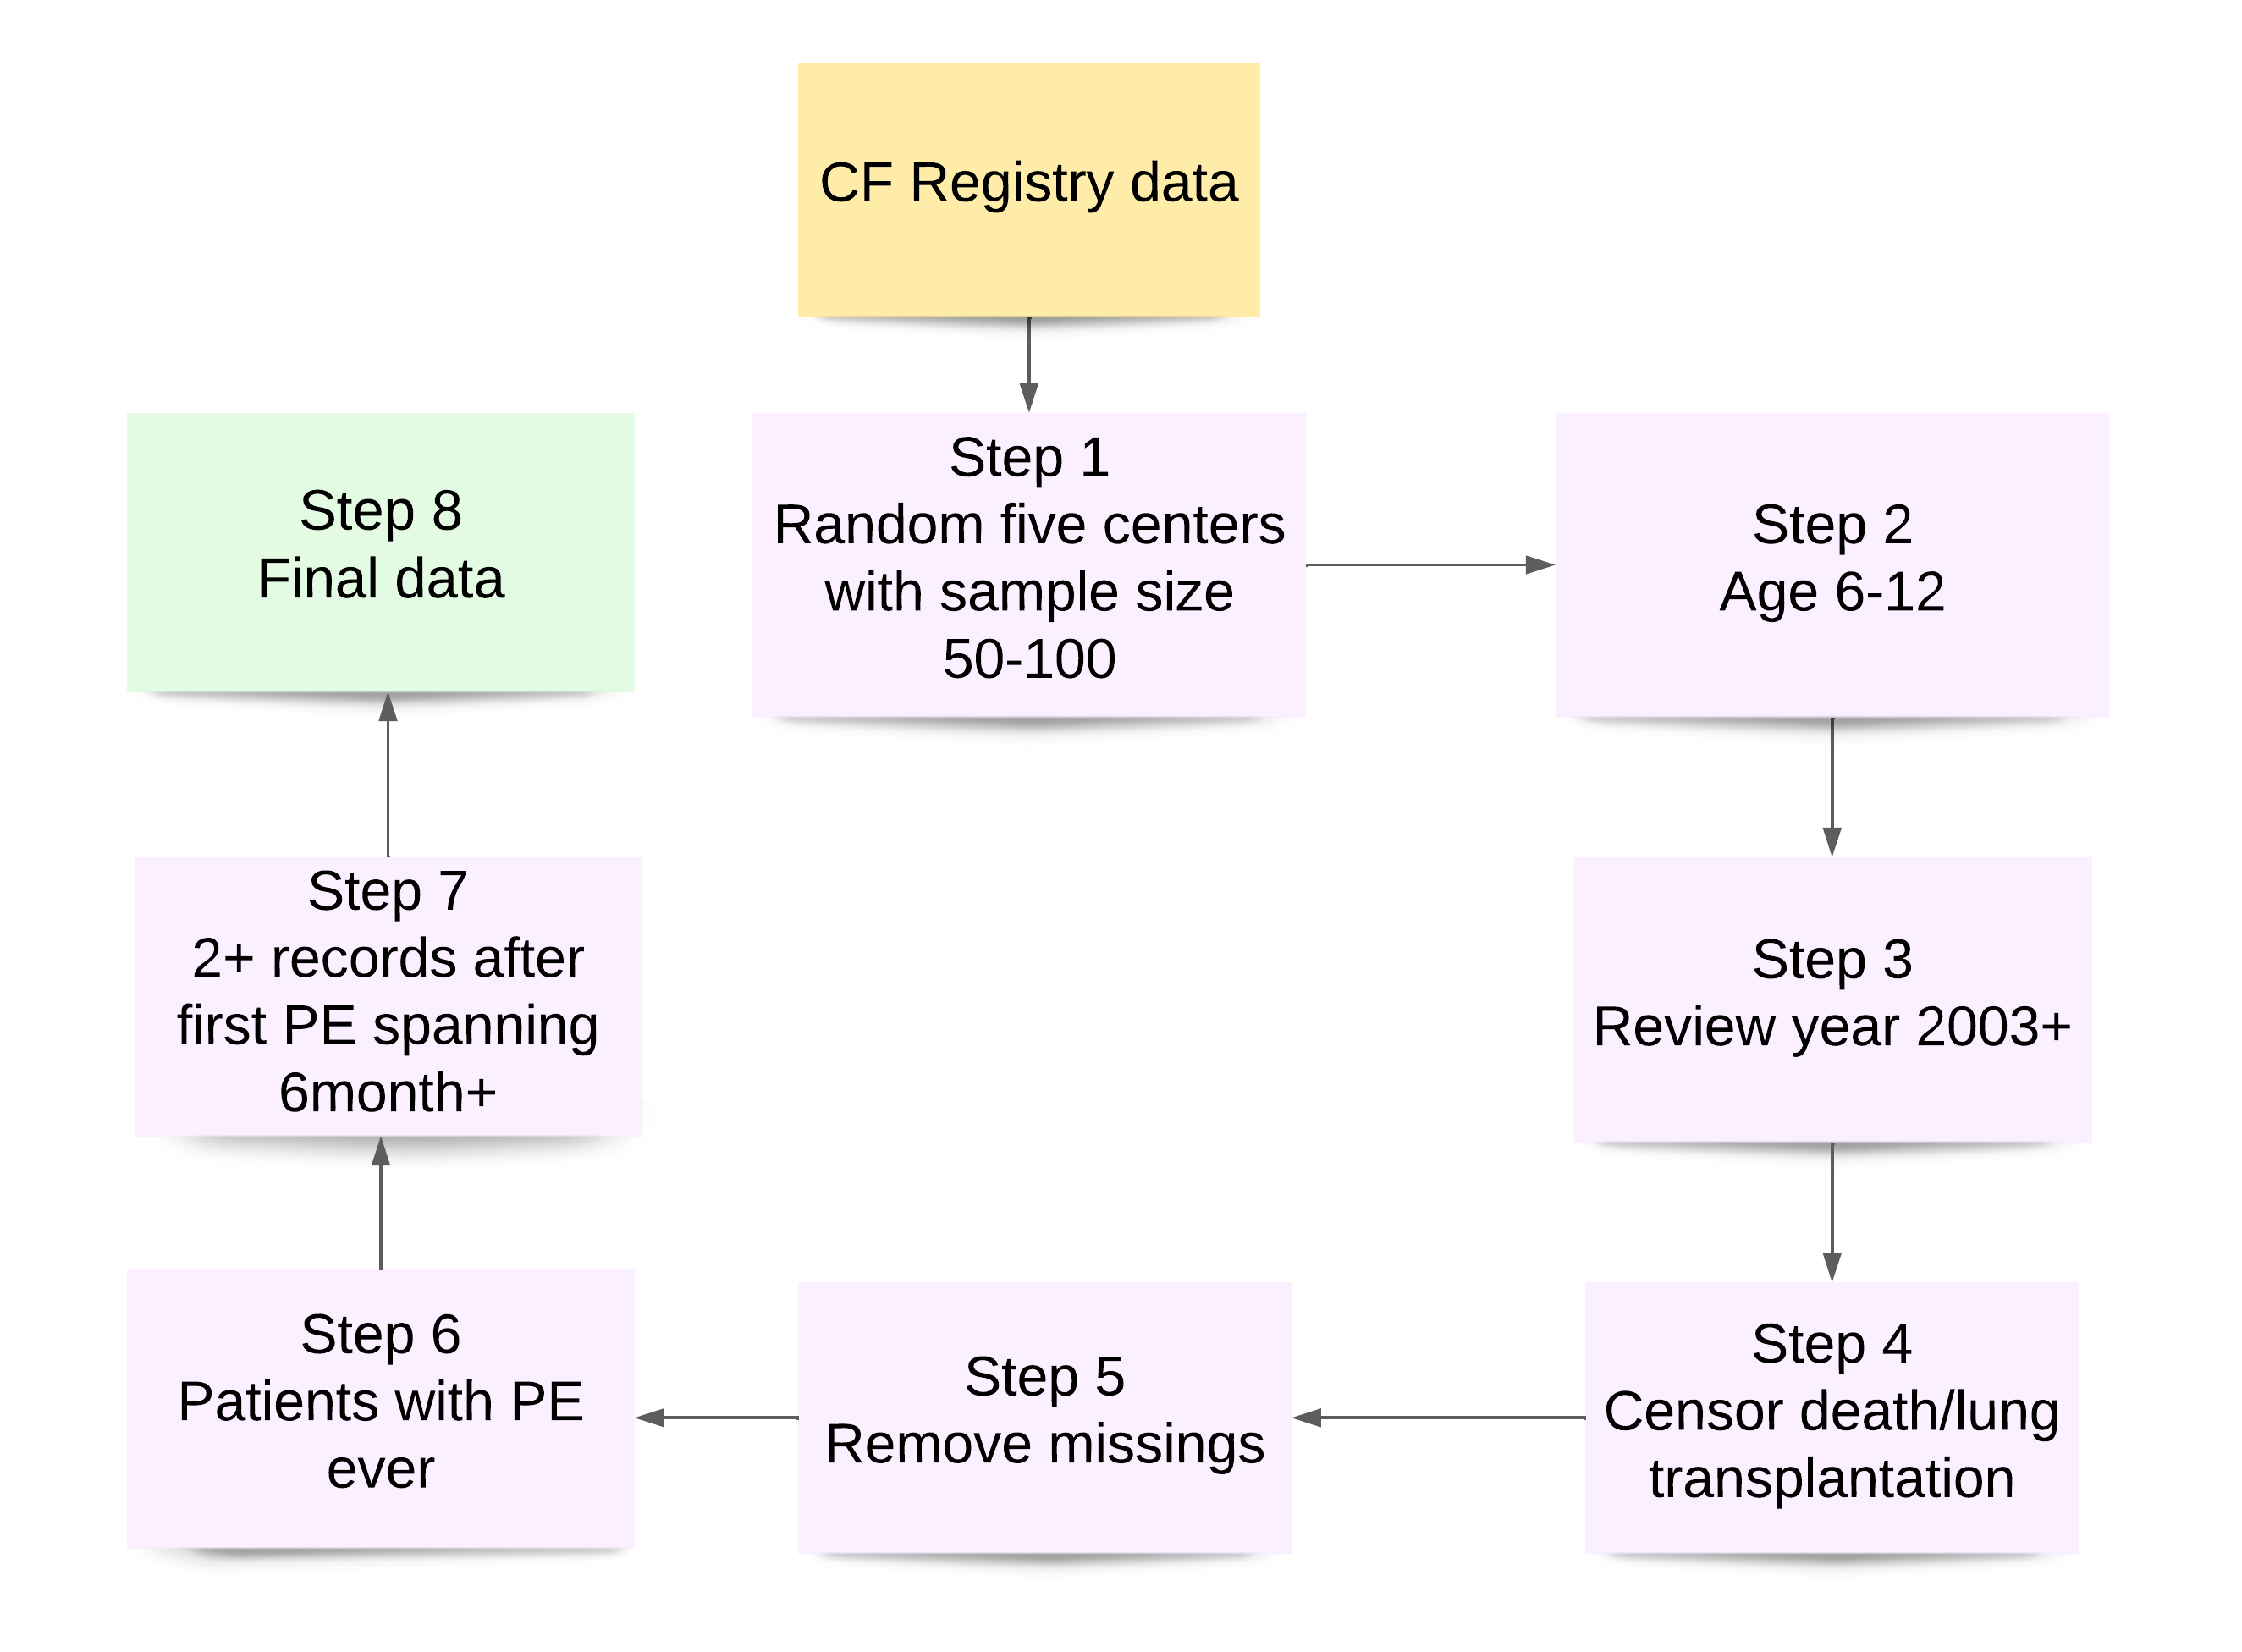
\includegraphics[width=\textwidth]{Figures/Chp2_app_dtclean.png}
\caption{Data cleaning process}
\end{figure}

\begin{center}
\begin{table}[H]
\caption{Clinical and demographic summary for CF data}
 \small
  \begin{tabular}{cccc}
    \toprule
 & Training Cohort (N=302) & Testing Cohort (N=79) & Total (N=381)\\
 \midrule 
   \multicolumn{4}{l}{\bf Center ID} \\
   \hline
   1 & 53 (17.5\%) & 14 (17.7\%) & 67 (17.6\%) \\
   2 & 81 (26.8\%) & 21 (26.6\%) & 102 (26.8\%) \\
   3 & 56 (18.5\%) & 15 (19.0\%) & 71 (18.6\%) \\
   4 & 77 (25.5\%) & 20 (25.3\%) & 97 (25.5\%) \\
   5 & 35 (11.6\%) & 9 (11.4\%) & 44 (11.5\%)\\
    \hline
   \multicolumn{4}{l}{\bf Genotpye (F508del)}\\
    \hline
   Homozygous & 176 (58.3\%) & 48 (60.8\%) & 224 (58.8\%) \\
   Heterozygous & 99 (32.8\%) & 26 (32.9\%) & 125 (32.8\%) \\
   Neither/unknown & 27 (8.9\%) & 5 (6.3\%) & 32 (8.4\%) \\
    \hline
 \multicolumn{4}{l}{\bf Age at baseline (years)}\\
  
 Mean; Median (Min - Max) & 7.94; 7.65 (6.0 - 11.4) & 7.76; 7.34 (6.0 - 11.1) & 7.90; 7.56 (6.0 - 11.4) \\
  
   \multicolumn{4}{l}{\bf ppFEV1 at baseline}\\
  
  Mean; Median (Min - Max) & 86.7; 88.2 (32.1 - 148) & 79.1; 79.3 (30.0 - 126) & 85.1; 87.3 (30.0 - 148) \\

  \multicolumn{4}{l}{\bf BMI percentile}\\
  Mean; Median (Min - Max) & 49.8; 51.0 (0.08 - 98.9) & 48.3; 49.2 (0.07 - 98.5) & 49.5; 50.4 (0.07 - 98.9) \\
  \hline
 \multicolumn{4}{l}{\bf  Insurance}\\
  \hline
  At baseline & 207 (68.5\%) & 53 (67.1\%) & 260 (68.2\%) \\
  Ever during follow up & 246 (81.5\%) & 65 (82.3\%) & 311 (81.6\%) \\
  \hline
  \multicolumn{4}{l}{\bf Pseudomonas aeruginosa (pa)}\\
   \hline
  At baseline & 52 (17.2\%) & 11 (13.9\%) & 63 (16.5\%) \\
  Ever during follow up & 206 (68.2\%) & 50 (63.3\%) & 256 (67.2\%)\\
  \hline
\multicolumn{4}{l}{\bf Methicillin-resistant Staphylococcus aureus (MRSA)} \\
 \hline
At baseline & 52 (17.2\%) & 11 (13.9\%) & 63 (16.5\%)\\
Ever during follow up & 206 (68.2\%) & 50 (63.3\%) & 256 (67.2\%)\\
\hline
\multicolumn{4}{l}{\bf Impaired CF-related diabetes mellitus (CFRD)} \\
 \hline
At baseline & 0 (0\%) 0 (0\%) 0 (0\%) \\
Ever during follow up & 33 (10.9\%) & 10 (12.7\%) & 43 (11.3\%)\\
\hline
\multicolumn{4}{l}{\bf Enzymes use} \\
 \hline
At baseline & 175 (57.9\%) & 44 (55.7\%) & 219 (57.5\%)\\
Ever during follow up & 294 (97.4\%) & 75 (94.9\%) & 369 (96.9\%)\\
\hline
\multicolumn{4}{l}{\bf Pulmonary Exacerbation (PE)} \\
 \hline
At baseline & 302 (100\%) & 79 (100\%) & 381 (100\%) \\
Ever during follow up & 296 (98.0\%) & 77 (97.5\%) & 373 (97.9\%)\\
    \bottomrule
  \end{tabular}
\end{table}
\label{tab:appb_dem}
\end{center}

\section{Convergence Diagnostics}

Figure \ref{fig:chp2_trace} shows that both chains explore the similar region of parameter values. We expect autocorrelation function (ACF) to drop quickly to zero with increasing lag because positive autocorrelation means the chain tends to stay in the same area between iterations. All parameters meet this expectation after lags $>$ 10 in Figure \ref{fig:chp2_acf}. The larger the ratio of $N_{\mbox{eff}}$ to $N$ the better (\cite{Gelman2013b}), a useful heuristic is to worry about any ratio less than 0.1 (\cite{StanManual}), which is not observed in Figure \ref{fig:chp2_eff}. 

\begin{figure}[H]
\centering
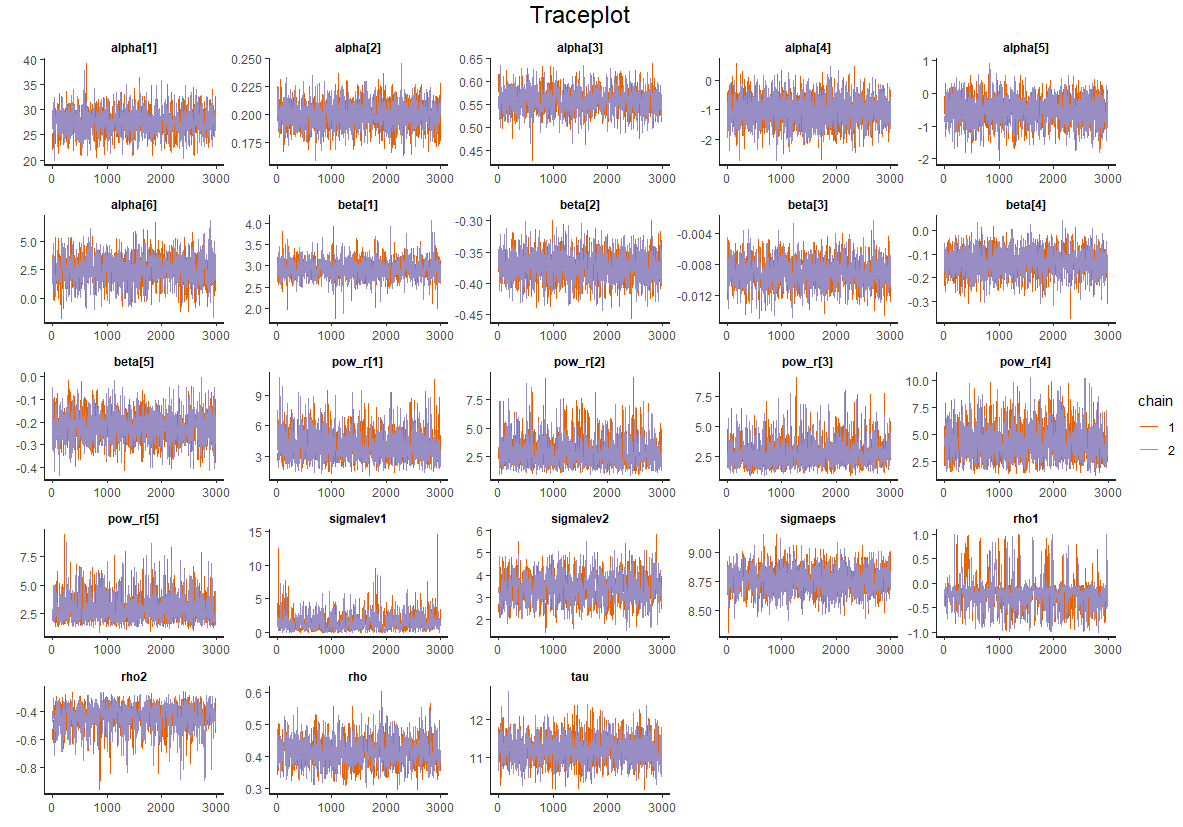
\includegraphics[width=0.9\textwidth]{Figures/Chp2_trace.png}
\caption{Traceplot for spep-$\mbox{JM}_4$}
\label{fig:chp2_trace}
\end{figure}

\begin{figure}[H]
\centering
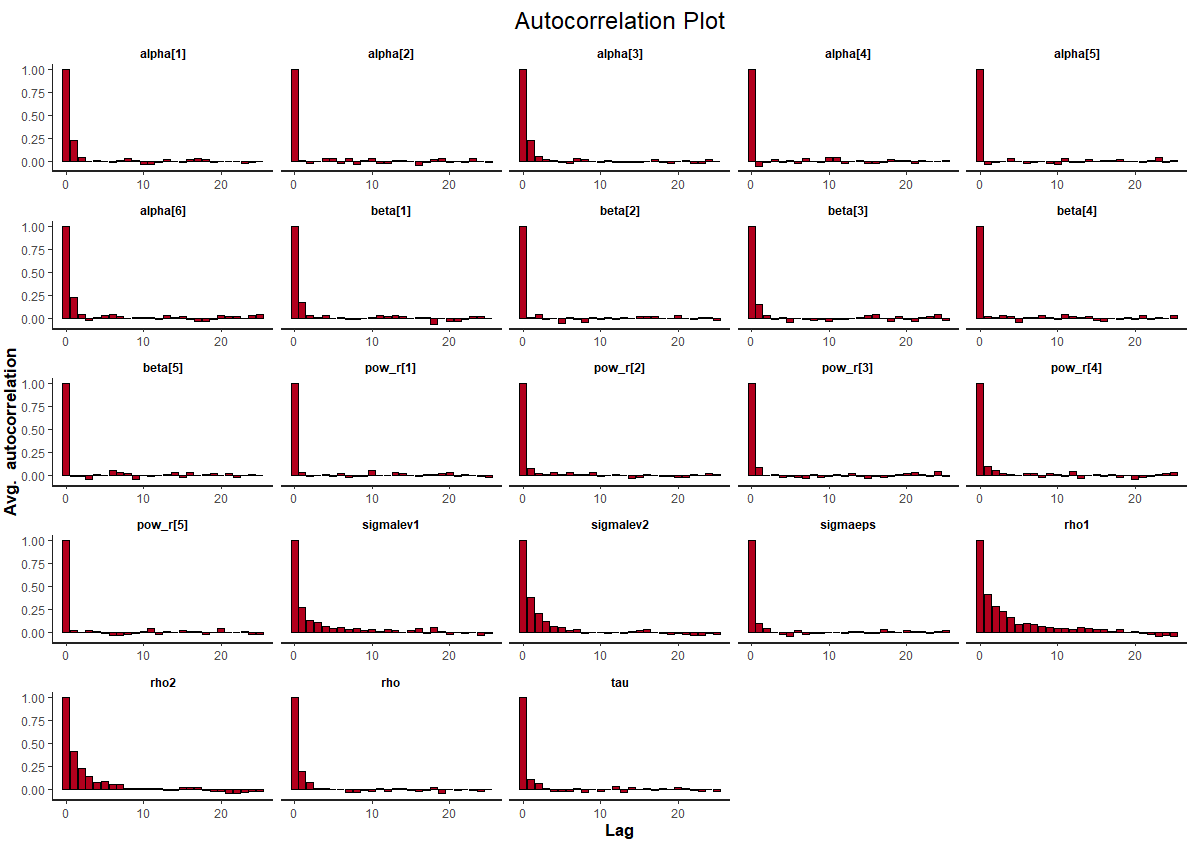
\includegraphics[width=0.9\textwidth]{Figures/Chp2_acf.png}
\caption{Autocorrelation plot for spep-$\mbox{JM}_4$}
\label{fig:chp2_acf}
\end{figure}

\begin{figure}[H]
\centering
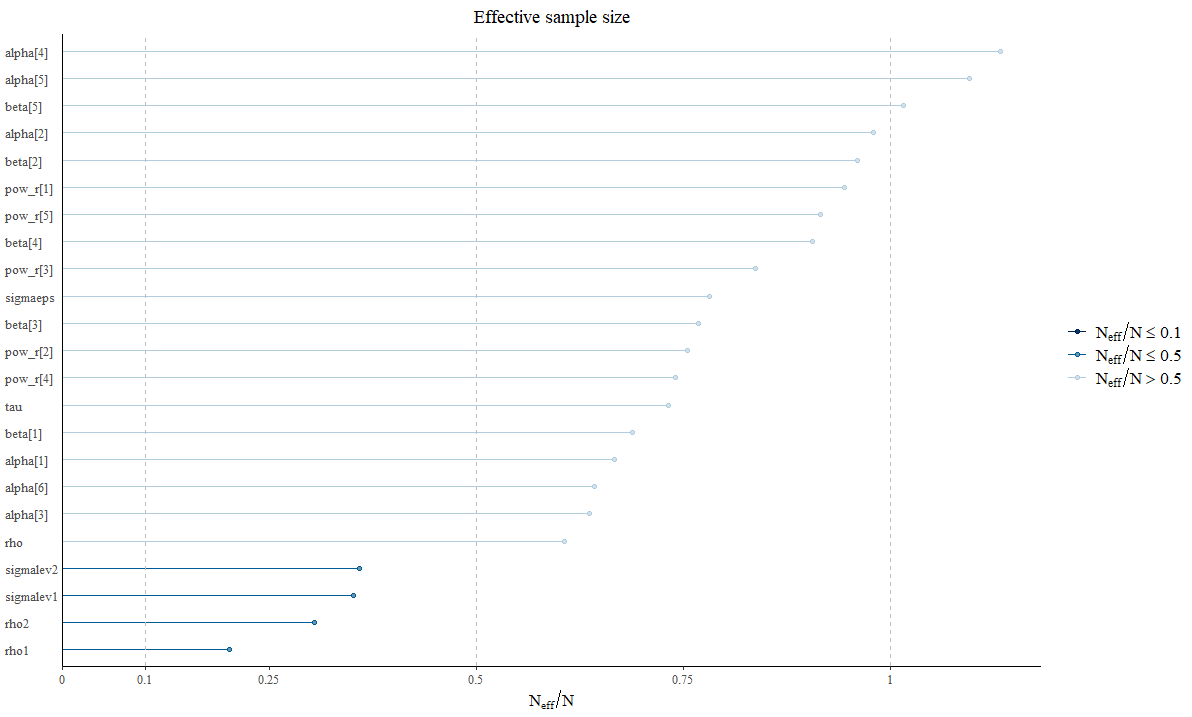
\includegraphics[width=0.9\textwidth]{Figures/Chp2_eff.png}
\caption{Effective sample size plot for spep-$\mbox{JM}_4$}
\label{fig:chp2_eff}
\end{figure}


\section{Residual Diagnostics}

To access residual diagnostics from the longitudinal submodel, we adapt to the method addressed in \cite{Diggle2015}, \cite{Szczesniak2020}. The standardized empirical marginal residual is given by

\begin{align}
    \bm{r}^*_{li}=\bm{S}^{-1}_{li} \cdot \bm{r}_{li}
\end{align}
where $\bm{r}_{li}=\bm{Y}_{li}-\bm{X}_{li}\bm{\alpha}$ denotes a vector of raw residuals. Let $\widehat{\bm{V}}_{li}=(\hat{\sigma}^2_b+\hat{\sigma}^2_u)\bm{J}_{li}+ \hat{\tau}^2 \bm{R}_{li} + \hat{\sigma}^2 \bm{I}_{li}$ be the estimated variance-covariance matrix for $\bm{Y}_{li}$ and $\bm{J}_{li}$, $\bm{I}_{li}$ and $\bm{R}_{li}$ are defined in the Section \ref{sec:chp2_pred}. Decompose $\bm{V}_{li}$ by lower triangular matrix $\bm{S}_{li}$ such that $\bm{V}_{li}=\bm{S}_{li}\bm{S}_{li}^T$ to achieve $\bm{S}^{-1}_{li}$.  

No clear pattern or trend is detected from Figure \ref{fig:chp2_residual}. The zero mean of standardized residuals (upper-left \& right panel), symmetric bell-shaped distribution (lower-left panel) corroborate model assumptions. The quantile-quantile plot implies a slightly heavier tails than the standard normal distribution.

\begin{figure}[H]
\centering
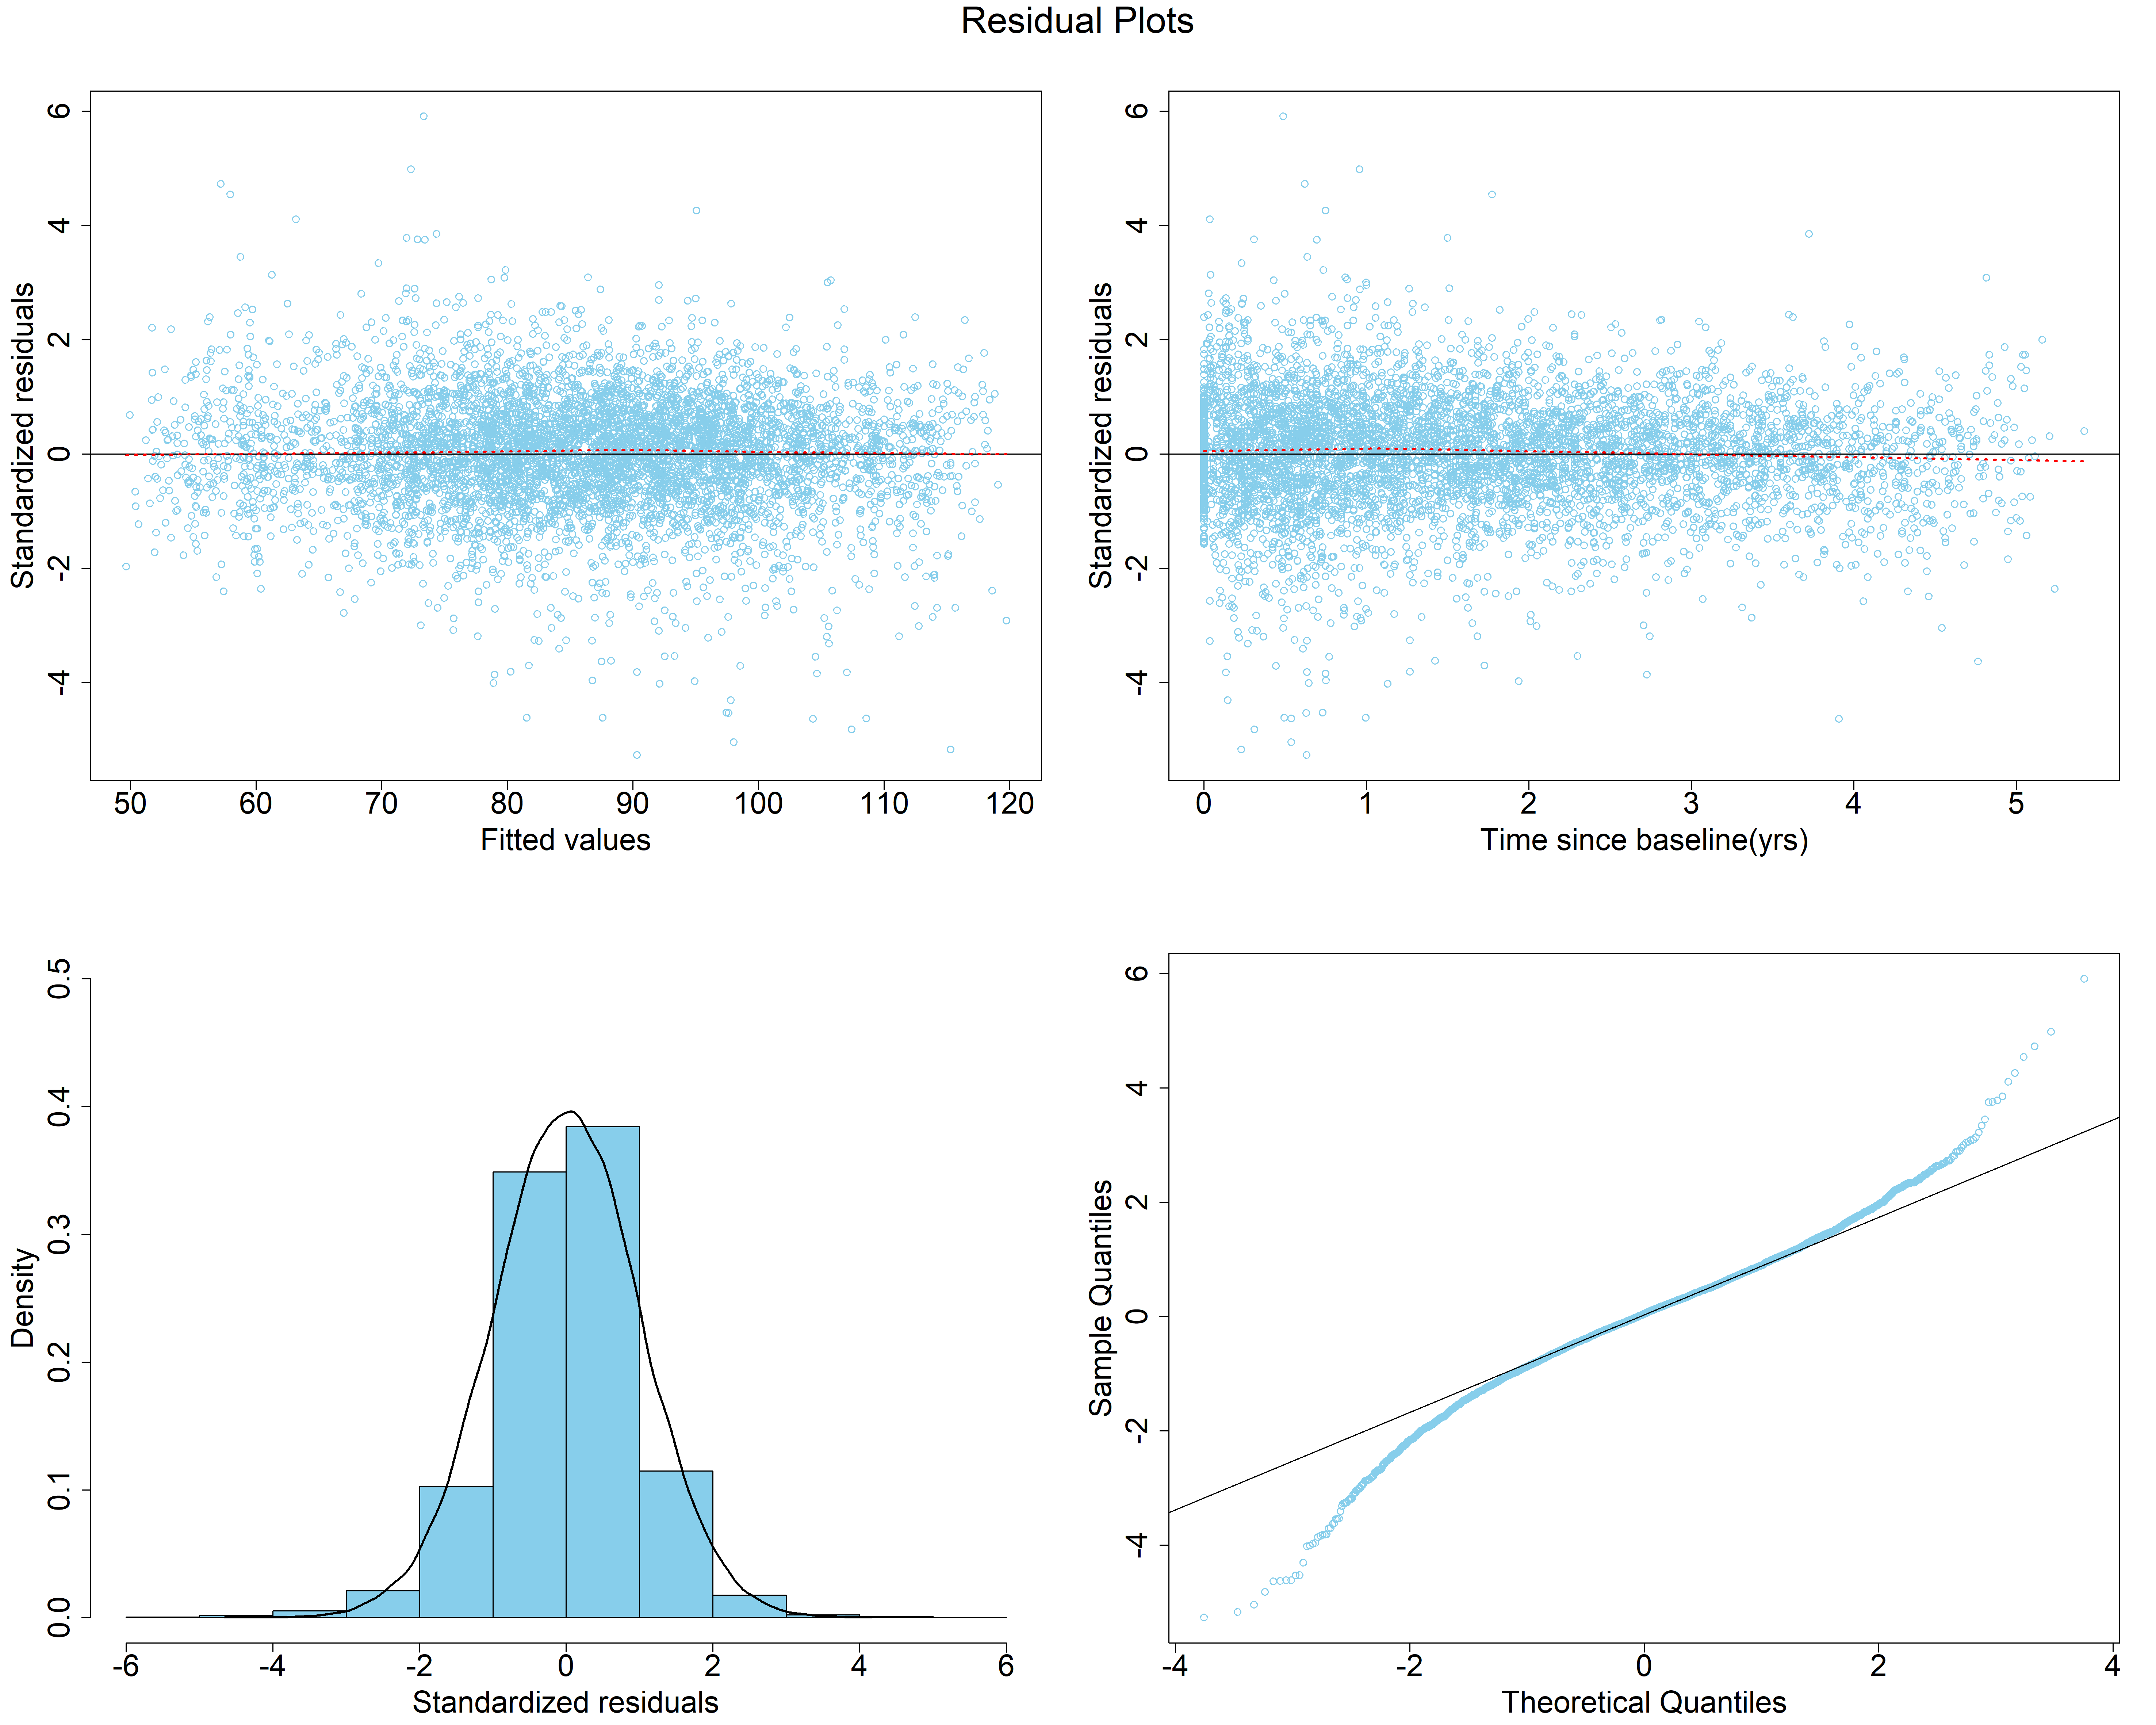
\includegraphics[width=0.9\textwidth]{Figures/Chp2_residual.png}
\caption{Diagnostics for standardized residuals from spep-JM4 based on Training Cohort: residuals vs. fitted values (upper left), residuals vs. time variable (upper right), histogram with standard normal density overlay (lower left) and quantile-quantile plot (lower right); LOWESS fitted curves (red dashed lines)}
\label{fig:chp2_residual}
\end{figure}


\section{Time and System}

\begin{center}
\begin{table}[H]
\caption{Averaged elapsed time for Simulation A with 50 replicates via CmdStanr}
 \centering \small
  \begin{threeparttable}
  \begin{tabular}{l|c|c|c}
    \toprule
Model & Time (mins) & Mac (mins/iter) & PC (mins/iter) \\
 \hline 
 logit-JM & 8.38 & 0.24 & 0.54 \\
 probit-JM & 10.30 & 0.29 & 0.68 \\
 cloglog-JM & 10.62 & 0.29 & 0.74 \\
 \bf splogit-JM & 15.35 & 0.39 & 1.14 \\
    \bottomrule
  \end{tabular}
  \begin{tablenotes}[para]
    \footnotesize
    Model in boldface: true model
    \end{tablenotes}
\end{threeparttable}
\end{table}
\label{tab:appb_simA}
\end{center}


\begin{center}
\begin{table}[H]
\caption{Averaged elapsed time for Simulation B with 50 replicates via RStan}
 \centering \small
 \begin{threeparttable}
  \begin{tabular}{l|l|c}
    \toprule
Model & Link & Time (hrs)  \\
 \hline 
 \multirow{2}{*}{Misspecified ($\mbox{JM}_1$)} & splogit & 9.88\\
                      & spep & 7.81\\
\hline
\multirow{2}{*}{No center-index ($\mbox{JM}_2$)} & splogit & 12.71\\
                      & spep & 10.93\\
\hline
\multirow{2}{*}{No covariance ($\mbox{JM}_3$)} & splogit & 9.51\\
                      & spep & 8.88\\
\hline
\multirow{2}{*}{\bf Proposed ($\mbox{JM}_4$)} & \bf splogit & 30.47\\
                      & \bf spep & 34.75\\                      
    \bottomrule
  \end{tabular}
   \begin{tablenotes}[para]
    \footnotesize
    Model in boldface: true model
    \end{tablenotes}
    \end{threeparttable}
\end{table}
\label{tab:appb_simB}
\end{center}

\begin{center}
\begin{table}[H]
\caption{Elapsed time for motivating data via RStan}
 \centering \small
 \begin{threeparttable}
  \begin{tabular}{l|c|c}
    \toprule
spep-Model & Time (hrs) & Iterations (post-warmup) \\
 \hline 
  Misspecified ($\mbox{JM}_1$) & 1.43 & 5000 \\
 No center-index ($\mbox{JM}_2$) & 2.86 & 8000 \\
 No covariance ($\mbox{JM}_3$) & 7.62 & 8000 \\
 \bf Proposed ($\mbox{JM}_4$) & 13.70 & 5000 \\
    \bottomrule
  \end{tabular}
   \begin{tablenotes}[para]
    \footnotesize
    Model in boldface: optimal model
    \end{tablenotes}
  \end{threeparttable}
\end{table}
\label{tab:appb_app}
\end{center}

\begin{table}[H] 
\centering\small
\caption{System information}
 \begin{threeparttable}
\begin{tabular}{c|c|c|c}
\toprule
 & \bf Mac & \bf PC & \bf BMI\\
\hline
Platform & x86\_64-apple-darwin17.0 (64-bit) & x86\_64-w64-mingw32/x64 (64-bit) & x86\_64-pc-linux-gnu\\
\hline
Running under & macOS Big Sur 10.16 & Windows 10 x64 (build 19043) & x86\_64, linux-gnu\\
\hline
R version & 4.0.5 (2021-03-31) & 4.0.2 (2020-06-22) & 3.6.1 (2019-07-05) \\
\hline
CmdStan & v2.28.2 & v2.29.1 & - \\
cmdstanr & v0.4.0 & v0.5.0 & - \\ 
rstan & - & - & 2.19.2 \\
\hline
\bottomrule
\end{tabular}
  \begin{tablenotes}[para]
    \footnotesize
   Note: i). Simulation A was implemented by both Mac and PC; ii) Simulation B and application study was implemented by Biomedical Informatics (BMI) at Cincinnati Children's Hospital
    \end{tablenotes}
 \end{threeparttable}
\label{tab:chp2_system}
\end{table}

\section{Example Codes}

\begin{SingleSpace}

\subsection{Stan Program}

\begin{minted}[breaklines]{R}

/***************************************************/
// Purpose: Fit proposed spep-JM4 in the manuscript  
// Author: Copyright (C) 2021, 2022 Grace C. Zhou
// Date: Apr., 2021
/***************************************************/

functions {

  //Define exponential power CDF expression
  
  real  spep_cdf(real x, real pow_r){
  
    if(pow_r <= 1){
		
		return(pow(double_exponential_cdf(x/pow_r, 0, 1), pow_r)); 
		
	} else { 
	
		return(1-pow(double_exponential_cdf(-pow_r * x, 0, 1), (1/pow_r))); 
		
	 }	
  }
}

data {
  
    int<lower=1> Nobs; //num obs 
    int<lower=1> N; //num patients
    
    int<lower=1> start_pos[N+1]; //starting point index
    int<lower=1> T[N]; //number obs per patient
    vector[Nobs] t; //time since first PE
    
    int<lower=1> NpredsX; //num LME predictors
    int<lower=1> NpredsV; //num GLMM predictors
    row_vector[NpredsX] X[Nobs]; // fix design matrix
    row_vector[NpredsV] V[Nobs]; // fix design matrix 
    
    int<lower=1> Nlev1; // num center
    int<lower=1,upper=Nlev1> levind1[Nobs]; //center index
    int<lower=1,upper=N> levind2[Nobs];// patient index
    vector[Nobs] y; //continuous outcome
    int r[Nobs]; //binary outcome
    real<lower=0> sdscal; //overall residual
   
}

parameters {
	
    vector[NpredsX] alpha; //fixed LME coefs 
    vector[NpredsV] beta; //fixed GLMM coefs 
    real<lower=0> sigmalev1; // center sd 
    real<lower=0> sigmalev2; // patient sd 
    real<lower=0> sigmaeps; // epsilon sd 
    real<lower=0> tau; // exp corr scale
    real<lower=0> rho; // exp corr 1/range 
    vector[Nlev1] eta1; //latent center
    vector[N] eta2; //latent patient
    vector[Nobs] eta; //latent exp corr
    real<lower = -1, upper = 1> rho1; // assoc center param
    real<lower = -1, upper = 1> rho2; // assoc patient param
    real<lower=0> pow_r[Nlev1]; //power parameter 
	
}

transformed parameters {
		
    vector[Nobs] w; // Gaussian process
    vector[Nobs] yhat; // linear predictor
    vector[Nlev1] ran1; // center effect
    vector[N] ran2; // patient effect
    vector[Nobs] Fsp; // response prob

    for (n in 1:N){
    
        matrix[T[n],T[n]] Sigma;
        matrix[T[n],T[n]] L_Sigma;
        vector[T[n]] t_sub;
        t_sub=t[start_pos[n]:(start_pos[n+1]-1)];
    		
        //off-diagonal elements
        for(i in 1:(T[n]-1)){
             for (j in (i+1):T[n]){
                Sigma[i,j] = pow(tau,2) * exp(- rho * fabs(t_sub[i] - t_sub[j]));
                Sigma[j,i] = Sigma[i,j];
          }
        }
    
       // diagonal elements
        for (k in 1:T[n]){
    	    Sigma[k,k] = pow(tau,2)+0.000001; // + jitter
        }
    		
        L_Sigma=cholesky_decompose(Sigma);
        w[start_pos[n]:(start_pos[n+1]-1)]= L_Sigma  * eta[start_pos[n]:(start_pos[n+1]-1)];
    }
    
    ran1 = sigmalev1 * eta1;
    ran2 = sigmalev2 * eta2;

    for(i in 1:Nobs){
        yhat[i] = X[i] * alpha + ran1[levind1[i]]  + ran2[levind2[i]] + w[i];
    	Fsp[i]=spep_cdf(V[i] * beta + rho1 * ran1[levind1[i]] + rho2 * ran2[levind2[i]], pow_r[levind1[i]]);		
    }
}

model {

    //----priors
    alpha ~ normal(0, 100); 
    beta ~ normal(0, 100);
    eta1 ~ normal(0,1);
    eta2 ~ normal(0,1);
    eta ~ normal(0,1);
    sigmalev1 ~ cauchy(0, 5);
    sigmalev2 ~ cauchy(0, 5);
    sigmaeps ~ cauchy(0, 2.5*sdscal);
    rho1 ~ uniform(-1, 1);
    rho2 ~ uniform(-1, 1);
    pow_r ~ exponential(1);
    tau ~ normal(0, 5);
    rho ~ inv_gamma(2,1);

    //----likelihood
    
    y ~ normal(yhat,sigmaeps);
    r ~ bernoulli(Fsp);
  
}

generated quantities{

    vector[Nobs] log_lik_y; 
    vector[Nobs] log_lik_r; 
  
  for (i in 1:Nobs){
      
	  log_lik_y[i] = normal_lpdf(y[i] | yhat[i], sigmaeps);
	  log_lik_r[i] = bernoulli_lpmf(r[i] | Fsp[i]);
	
  }
  
}

\end{minted}

\subsection{R Code}

\begin{minted}[breaklines]{R}

library(rstan)
rstan::rstan_options(auto_write = TRUE)
options(mc.cores = parallel::detectCores())

#read in STAN code
Stan.SPEP<-stan_model(stanc_ret=stanc("SPEP_JM4.stan"),verbose=FALSE) 

FIT.JM4.SPEP<-sampling(Stan.SPEP,data=JD,warmup=2000,iter=5000,thin=3,chains=2, control=list(adapt_delta=0.95,max_treedepth=15), 
              seed=1781002850, init_r=0.2,
              save_warmup=FALSE)

\end{minted}

\end{SingleSpace}
\chapter{Appendix for Chapter \ref{chp3}} \label{app:c}

\section{Conditional Survival Probability}

\begin{flalign}
 S_{li}(t'|t) & = p(t_{n_{li}+1} \geq t'|t_{n_{li}+1} > t,\mathcal{D})&&\\\nonumber
              & = \int\int\int\int p(t_{n_{li}+1} \geq t'|t_{n_{li}+1} > t, b_l,\bm{U}_{li},v_{li},\bm{\theta},\mathcal{D}) \cdot p(b_l, \bm{U}_{li}, v_{li}, \bm{\theta} |t_{n_{li}+1} > t, \mathcal{D}) \, db_l \, d\bm{U}_{li} \, dv_{li} \, d\bm{\theta}&& \nonumber \\
              & = \int\int\int\int \frac{p(t_{n_{li}+1} \geq t'|b_l, \bm{U}_{li}, v_{li}, \bm{\theta})}{p(t_{n_{li}+1} > t|b_l, \bm{U}_{li}, v_{li}, \bm{\theta})} \cdot p(b_l, \bm{U}_{li}, v_{li}, \bm{\theta} |t_{n_{li}+1} > t, \mathcal{D}) \, db_l \, d\bm{U}_{li} \, dv_{li} \, d\bm{\theta}&& \nonumber \\
              & = \int\int\int\int \frac{S(t'|b_l, \bm{U}_{li}, v_{li}, \bm{\theta})}{S(t|b_l, \bm{U}_{li}, v_{li}, \bm{\theta})} \cdot p(b_l, \bm{U}_{li}, v_{li}, \bm{\theta} |t_{n_{li}+1} > t, \mathcal{D}) \, db_l \, d\bm{U}_{li} \, dv_{li} \, d\bm{\theta}&& \nonumber \\
              &=\int\int\int\int \frac{exp\Big[-\int_{0}^{t'}h(s|b_l, \bm{U}_{li}, v_{li}, \bm{\theta})ds\Big]}{exp\Big[-\int_{0}^{t}h(s|b_l, \bm{U}_{li}, v_{li}, \bm{\theta})ds\Big]} \cdot p(b_l, \bm{U}_{li}, v_{li}, \bm{\theta} |t_{n_{li}+1} > t, \mathcal{D}) \, db_l \, d\bm{U}_{li} \, dv_{li} \, d\bm{\theta}&& \nonumber \\
              &=\int\int\int\int exp\Big[-\int_{t}^{t'}h(s|b_l, \bm{U}_{li}, v_{li}, \bm{\theta})ds\Big] \cdot p(b_l, \bm{U}_{li}, v_{li}, \bm{\theta} |t_{n_{li}+1} > t, \mathcal{D}) \, db_l \, d\bm{U}_{li} \, dv_{li} \, d\bm{\theta}&& \nonumber \\
              & \approx \frac{1}{M} \sum_{m=1}^{M} exp\Big[ -\int_t^{t'} h\big(s|b_l^{(m)},\bm{U}_{li}^{(m)},v_{li}^{(m)},\bm{\theta}^{(m)}\big) ds \Big] \nonumber
\end{flalign}

\section{Simulation Results}

\begin{center}
\begin{table}[H]
\caption{Simulation results under models with current slope as association structure across gap \& calendar risk intervals}
 \centering
 \begin{threeparttable}
  \begin{tabular}{lrllrllrllrll}
    \toprule
   & \multicolumn{6}{c} {SLOPE+GAP} & \multicolumn{6}{c} {SLOPE+CAL}\\
    \cmidrule(lr) {2-7} 
    \cmidrule(lr) {8-13} 
  Parameter & \multicolumn{3}{c}{Joint Model} & \multicolumn{3}{c}{Two-stage Model} & \multicolumn{3}{c}{Joint Model} & \multicolumn{3}{c}{Two-stage Model}  \\
 \cmidrule(lr) {2-4}  \cmidrule(lr) {5-7}
 \cmidrule(lr) {8-10}  \cmidrule(lr) {11-13}
 & Bias \tnote{a} & SE \tnote{b} & C90 \tnote{c} & Bias \tnote{a} & SE \tnote{b} & C90 \tnote{c} & Bias \tnote{a} & SE \tnote{b} & C90 \tnote{c} & Bias \tnote{a} & SE \tnote{b} & C90 \tnote{c} \\
 \midrule 
 \rowcolor{Gainsboro!60}
 \multicolumn{13}{l}{\bf Longitudinal submodel}\\
  $\beta_0$ & -0.20 & 0.36 & 0.86 & -0.24 & 0.37 & 0.86 & 0.23 & 0.32 & 0.92 & 0.18 & 0.32 & 0.92\\
  $\beta_1$ & 0.02 & 0.05 & 0.94 & -0.11 & 0.06 & 0.92 & 0.09 & 0.06 & 0.88 & 0.10 & 0.07 & 0.84\\
  $\beta_2$ & -0.01 & 0.01 & 0.94 & 0.01 & 0.01 & 0.90 & -0.01 & 0.01 & 0.88 & 0.00 & 0.01 & 0.88\\
  $\sigma$ & -0.19 & 0.06 & 0.90 & -0.18 & 0.06 & 0.90 & -0.07 & 0.06 & 0.90 & -0.03 & 0.06 & 0.90\\
  $\sigma_b$ & -0.42 & 0.25 & 0.98 & -0.39 & 0.24 & 0.98 & -0.20 & 0.28 & 0.98 & -0.21 & 0.28 & 0.96\\
  $\sigma_{u0}$ & 0.06 & 0.11 & 0.94 & 0.09 & 0.11 & 0.94 & -0.12 & 0.11 & 0.92 & -0.14 & 0.12 & 0.92\\
  $\sigma_{u1}$ & 0.04 & 0.02 & 0.92 & 0.03 & 0.02 & 0.90 & 0.01 & 0.02 & 0.96 & -0.01 & 0.02 & 0.96\\
  $\rho$ & -0.01 & 0.01 & 0.90 & -0.01 & 0.01 & 0.94 & 0.00 & 0.01 & 0.84 & 0.01 & 0.01 & 0.86\\
  \rowcolor{Gainsboro!60}
  \multicolumn{13}{l}{\bf Event submodel}\\
  $\gamma_0$ & 0.38 & 0.07 & 0.70 & 0.32 & 0.06 & 0.68 & 0.22 & 0.04 & 0.82 & 0.20 & 0.04 & 0.80\\
  $\gamma_1$ & 0.01 & 0.04 & 0.88 & 0.00 & 0.04 & 0.88 & -0.03 & 0.03 & 0.96 & -0.03 & 0.03 & 0.96\\
  $\gamma_2$ & 0.03 & 0.02 & 0.90 & 0.03 & 0.02 & 0.90 & 0.03 & 0.02 & 0.90 & 0.03 & 0.02 & 0.90\\
  $\delta_1$ & -0.08 & 0.02 & 0.84 & -0.07 & 0.02 & 0.84 & -0.03 & 0.02 & 0.86 & -0.02 & 0.02 & 0.88\\
  $\delta_2$ & -0.05 & 0.02 & 0.90 & -0.04 & 0.02 & 0.90 & -0.01 & 0.02 & 0.90 & -0.01 & 0.02 & 0.78\\
  $\delta_3$ & -0.10 & 0.03 & 0.80 & -0.07 & 0.03 & 0.82 & -0.02 & 0.02 & 0.94 & -0.02 & 0.02 & 0.94\\
  $\delta_4$ & -0.08 & 0.03 & 0.84 & -0.05 & 0.03 & 0.84 & 0.01 & 0.02 & 0.94 & 0.01 & 0.02 & 0.94\\
  $\delta_5$ & -0.06 & 0.02 & 0.88 & -0.05 & 0.02 & 0.90 & 0.00 & 0.03 & 0.90 & 0.01 & 0.03 & 0.88\\
  $\delta_6$ & -0.07 & 0.02 & 0.88 & -0.05 & 0.02 & 0.88 & -0.04 & 0.03 & 0.88 & -0.04 & 0.02& 0.90\\
  $\alpha_1$ & 0.02 & 0.01 & 0.88 & 0.01 & 0.01 & 0.84 & 0.01 & 0.01 & 0.98 & 0.01 & 0.01 & 0.94\\
  $\alpha_2$ & 0.01 & 0.01 & 0.88 & 0.00 & 0.01 & 0.88 & 0.02 & 0.01 & 0.94 & 0.02 & 0.01 & 0.92\\
  $\alpha_3$ & -0.02 & 0.02 & 0.86 & -0.01 & 0.02 & 0.86 & 0.02 & 0.02 & 0.86 & 0.02 & 0.02 & 0.86\\
  $\alpha_4$ & -0.05 & 0.02 & 0.86 & -0.04 & 0.02 & 0.84 & 0.00 & 0.02 & 0.94 & 0.00 & 0.02 & 0.92\\
  $\alpha_5$ & -0.03 & 0.02 & 0.86 & -0.03 & 0.02 & 0.88 & 0.01 & 0.01 & 0.94 & 0.01 & 0.01 & 0.96\\
  $\alpha_6$ & -0.01 & 0.02 & 0.86 & -0.01 & 0.02 & 0.90 & -0.01 & 0.01 & 0.92 & -0.01 & 0.01 & 0.92\\
  $\sigma_v$ & -0.14 & 0.02 & 0.76 & -0.15 & 0.02 & 0.78 & -0.08 & 0.02 & 0.90 & -0.10 & 0.02 & 0.92\\
    \bottomrule
  \end{tabular}
   \begin{tablenotes}[para]
    \footnotesize
        \item[a] Bias=true value-mean estimate; \item[b] SE=standard error; \item[c] C90= probability of 90\% coverage 
    \end{tablenotes}
    \end{threeparttable}
\end {table}
\end{center}

\begin{center}
\begin{table}[H]
\caption{Simulation results under models with current value as association structure across gap \& calendar risk intervals}
 \centering
 \begin{threeparttable}
  \begin{tabular}{lrllrllrllrll}
    \toprule
   & \multicolumn{6}{c} {VALUE+GAP} & \multicolumn{6}{c} {VALUE+CAL}\\
    \cmidrule(lr) {2-7} 
    \cmidrule(lr) {8-13} 
  Parameter & \multicolumn{3}{c}{Joint Model} & \multicolumn{3}{c}{Two-stage Model} & \multicolumn{3}{c}{Joint Model} & \multicolumn{3}{c}{Two-stage Model}  \\
 \cmidrule(lr) {2-4}  \cmidrule(lr) {5-7}
 \cmidrule(lr) {8-10}  \cmidrule(lr) {11-13}
 & Bias \tnote{a} & SE \tnote{b} & C90 \tnote{c} & Bias \tnote{a} & SE \tnote{b} & C90 \tnote{c} & Bias \tnote{a} & SE \tnote{b} & C90 \tnote{c} & Bias \tnote{a} & SE \tnote{b} & C90 \tnote{c} \\
 \midrule 
 \rowcolor{Gainsboro!60}
 \multicolumn{13}{l}{\bf Longitudinal submodel}\\
  $\beta_0$ & 0.07 & 0.33 & 0.90 & 0.08 & 0.33 & 0.92 & -0.34 & 0.32 & 0.96 & -0.30 & 0.32 & 0.96\\
  $\beta_1$ & 0.05 & 0.06 & 0.96 & 0.20 & 0.06 & 0.90 & 0.00 & 0.05 & 0.92 & 0.11 & 0.06 & 0.92 \\
  $\beta_2$ & 0.00 & 0.01 & 0.86 & -0.02 & 0.01 & 0.84 & 0.00 & 0.01 & 0.94 & -0.02 & 0.01 & 0.90 \\
  $\sigma$ & -0.07 & 0.05 & 0.90 & -0.06 & 0.05 & 0.90 & 0.00 & 0.05 & 0.90 & 0.02 & 0.05 & 0.92 \\
  $\sigma_b$ & -0.12 & 0.30 & 0.96 & -0.18 & 0.28 & 0.96 & -0.94 & 0.28 & 0.90 & -0.89 & 0.28 & 0.92 \\
  $\sigma_{u0}$ & -0.13 & 0.11 & 0.94 & -0.15 & 0.11 & 0.94 & 0.00 &  0.11 & 0.92 & -0.05 & 0.11 & 0.92 \\
  $\sigma_{u1}$ & -0.01 & 0.02 & 0.98 & -0.02 & 0.02 & 0.98 & 0.01 &  0.02 & 0.94 & 0.00 & 0.02 & 0.92 \\
  $\rho$ & -0.01 & 0.01 & 0.94 & -0.01 & 0.01 & 0.94 & 0.01 & 0.01 &  0.94 & 0.01 & 0.01 & 0.96 \\
  \rowcolor{Gainsboro!60}
  \multicolumn{13}{l}{\bf Event submodel}\\
  $\gamma_0$ & 0.21 & 0.05 & 0.86 & 0.18 & 0.05 & 0.86 & 0.31 & 0.06 & 0.86 & 0.27 & 0.06 & 0.88\\
  $\gamma_1$ & -0.06 & 0.05 & 0.90 & -0.06 & 0.05 & 0.90 & -0.02 & 0.04 & 0.98 & -0.02 & 0.04 & 0.98 \\
  $\gamma_2$ & -0.03 & 0.02 & 0.96 & -0.03 & 0.02 & 0.96 & -0.04 & 0.02 & 0.92& -0.04 & 0.02 & 0.92\\
  $\delta_1$ & -0.11 & 0.03 & 0.90 & -0.10 & 0.03 & 0.86 & -0.06 & 0.03 & 0.82 & -0.05 & 0.03 & 0.80\\
  $\delta_2$ & -0.03 & 0.03 & 0.90 & -0.02 & 0.03 & 0.88 & 0.82 & 0.03 & 0.96 & -0.07 & 0.03 & 0.98\\
  $\delta_3$ & -0.07 & 0.02 & 0.90 & -0.06 & 0.02 & 0.92 & -0.04 & 0.03 & 0.92 & -0.04 & 0.03 & 0.92\\
  $\delta_4$ & -0.02 & 0.02 & 0.94 & -0.02 & 0.02 & 0.94 & -0.02 & 0.02 & 0.92 & -0.02 & 0.02 & 0.92\\
  $\delta_5$ & -0.06 & 0.02 & 0.88 & -0.06 & 0.02 & 0.92 & -0.05 & 0.02 & 0.96 & -0.05 & 0.02 & 0.96\\
  $\delta_6$ & -0.02 & 0.03 & 0.92 & -0.01 & 0.03 & 0.90 & -0.06 & 0.03 & 0.88 & -0.05 & 0.03 & 0.86\\
  $\alpha_1$ & 0.00 & 0.00 & 0.88 & 0.00 & 0.00 & 0.86 & 0.00 & 0.00 & 0.88 & 0.00 & 0.00 & 0.88\\
  $\alpha_2$ & 0.00 & 0.00 & 0.90 & 0.00 & 0.00 & 0.88 & 0.00 & 0.00 & 0.92 & 0.00 & 0.00 & 0.92\\
  $\alpha_3$ & 0.00 & 0.00 & 0.84 & 0.00 & 0.00 & 0.82 & 0.00 & 0.00 & 0.88 & 0.00 & 0.00 & 0.88\\
  $\alpha_4$ & 0.00 & 0.00 & 0.92 & 0.00 & 0.00 & 0.92 & 0.00 & 0.00 & 0.96 & 0.00 & 0.00 & 0.96\\
  $\alpha_5$ & 0.00 & 0.00 & 0.86 & 0.00 & 0.00 & 0.86 & 0.00 & 0.00 & 0.88 & 0.00 & 0.00 & 0.88\\
  $\alpha_6$ & 0.00 & 0.00 & 0.86 & 0.00 & 0.00 & 0.88 & 0.00 & 0.00 & 0.88 & 0.00 & 0.00 & 0.90\\
  $\sigma_v$ & -0.16 & 0.03 & 0.80 & -0.16 & 0.03 & 0.78 & -0.05 & 0.03 & 0.88 & -0.05 & 0.03 & 0.90\\
    \bottomrule
  \end{tabular}
   \begin{tablenotes}[para]
    \footnotesize
        \item[a] Bias=true value-mean estimate; \item[b] SE=standard error; \item[c] C90=probability of 90\% credible interval coverage 
    \end{tablenotes}
    \end{threeparttable}
\end {table}
\end{center}

\section{Real Data}

\begin{figure}[H]
\centering
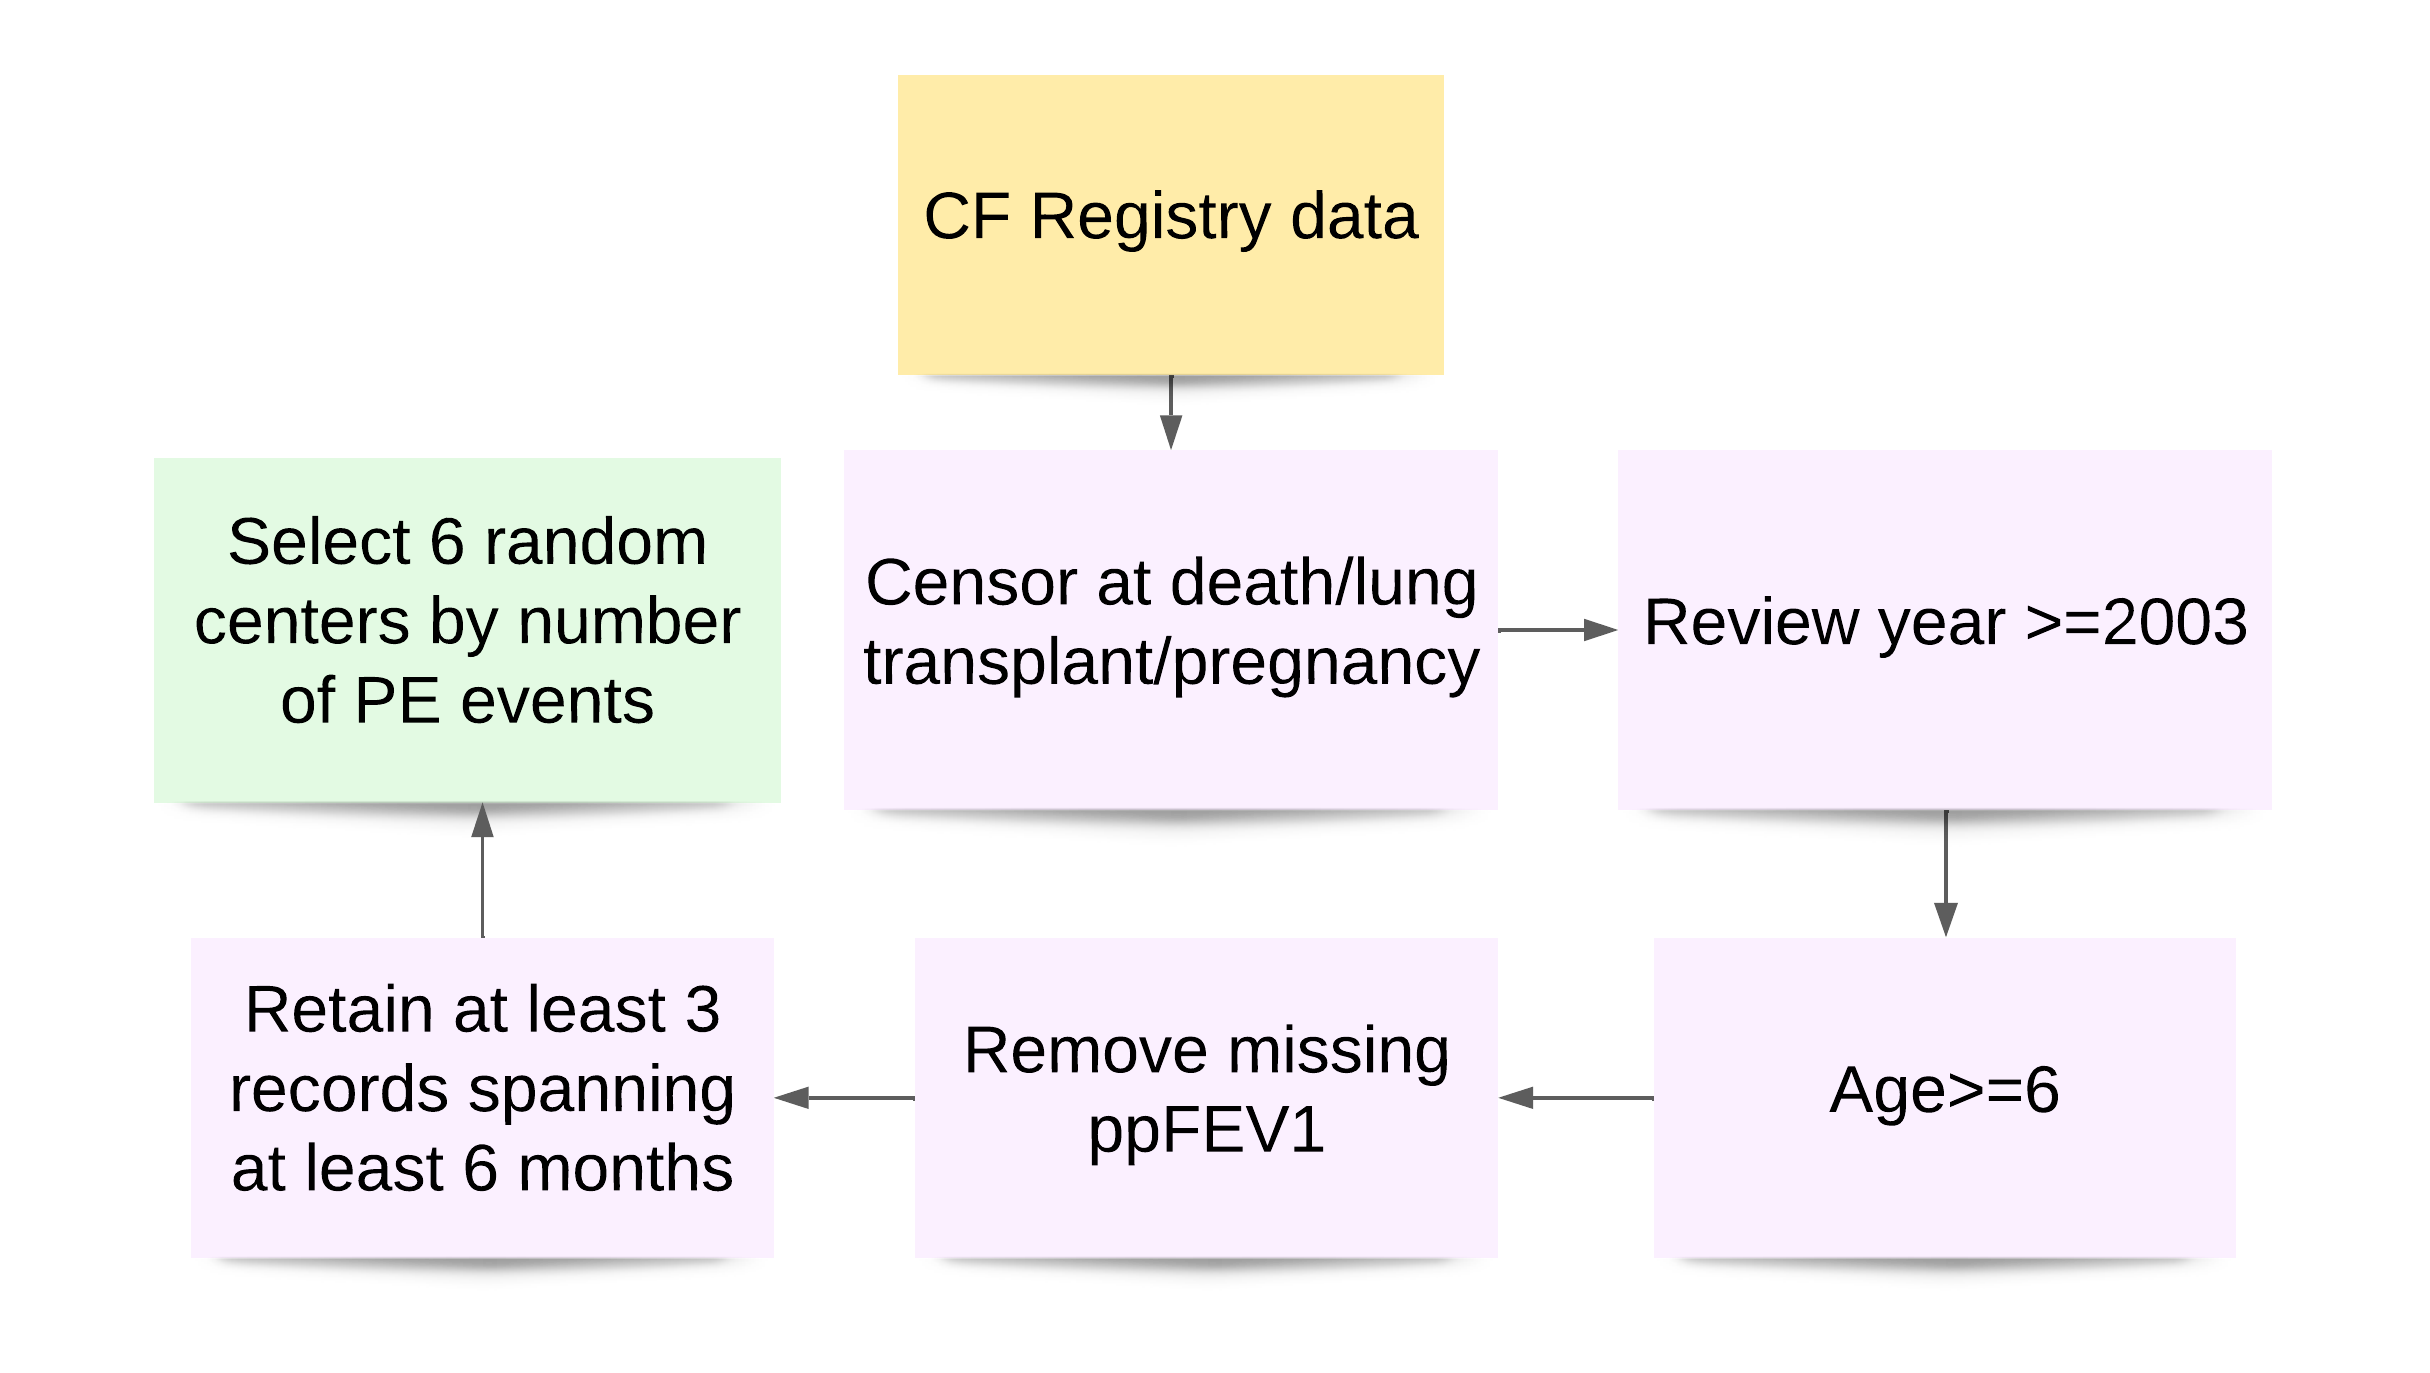
\includegraphics[width=\textwidth]{Figures/Chp3_data_diag.png}
\caption{Data cleaning process}
\end{figure}

\section{Convergence Diagnostics}

In this section, we have investigated some common visual MCMC diagnostics using the R bayesplot (\cite{bayesplot2020}) package for our optimal model. The time series plot of the Markov chains is shown in Figure \ref{fig:trace}. Typically we can see that both chains explore the similar region of parameter values, which is a good sign. We can also visualize the ACF for each Markov chain separately up to a lag of 20 for each parameter. We prefer ACF to drop quickly to zero with increasing lag because positive autocorrelation means the chain tends to stay in the same area between iterations. All parameters are shown to meet this expectation from Figure \ref{fig:acf_long} and Figure \ref{fig:acf_surv}. It is notable that negative autocorrelation is possible and it indicates fast convergence of sample mean towards true mean.  

The motivation of the potential scale reduction statistic($\hat{R}$) is to measure the ratio of the average variance of draws within each chain to the variance of pooled draws across chains. If the chains have not converged to a common distribution, the $\hat{R}$ statistic will be greater than one (\cite{Gelman2013b},\cite{Rstan2020}). The points in Figure \ref{fig:rhat} representing $\hat{R}$ values are colored based on some cutoffs and there are no divergences observed.   

\begin{figure}[H] 
\centering
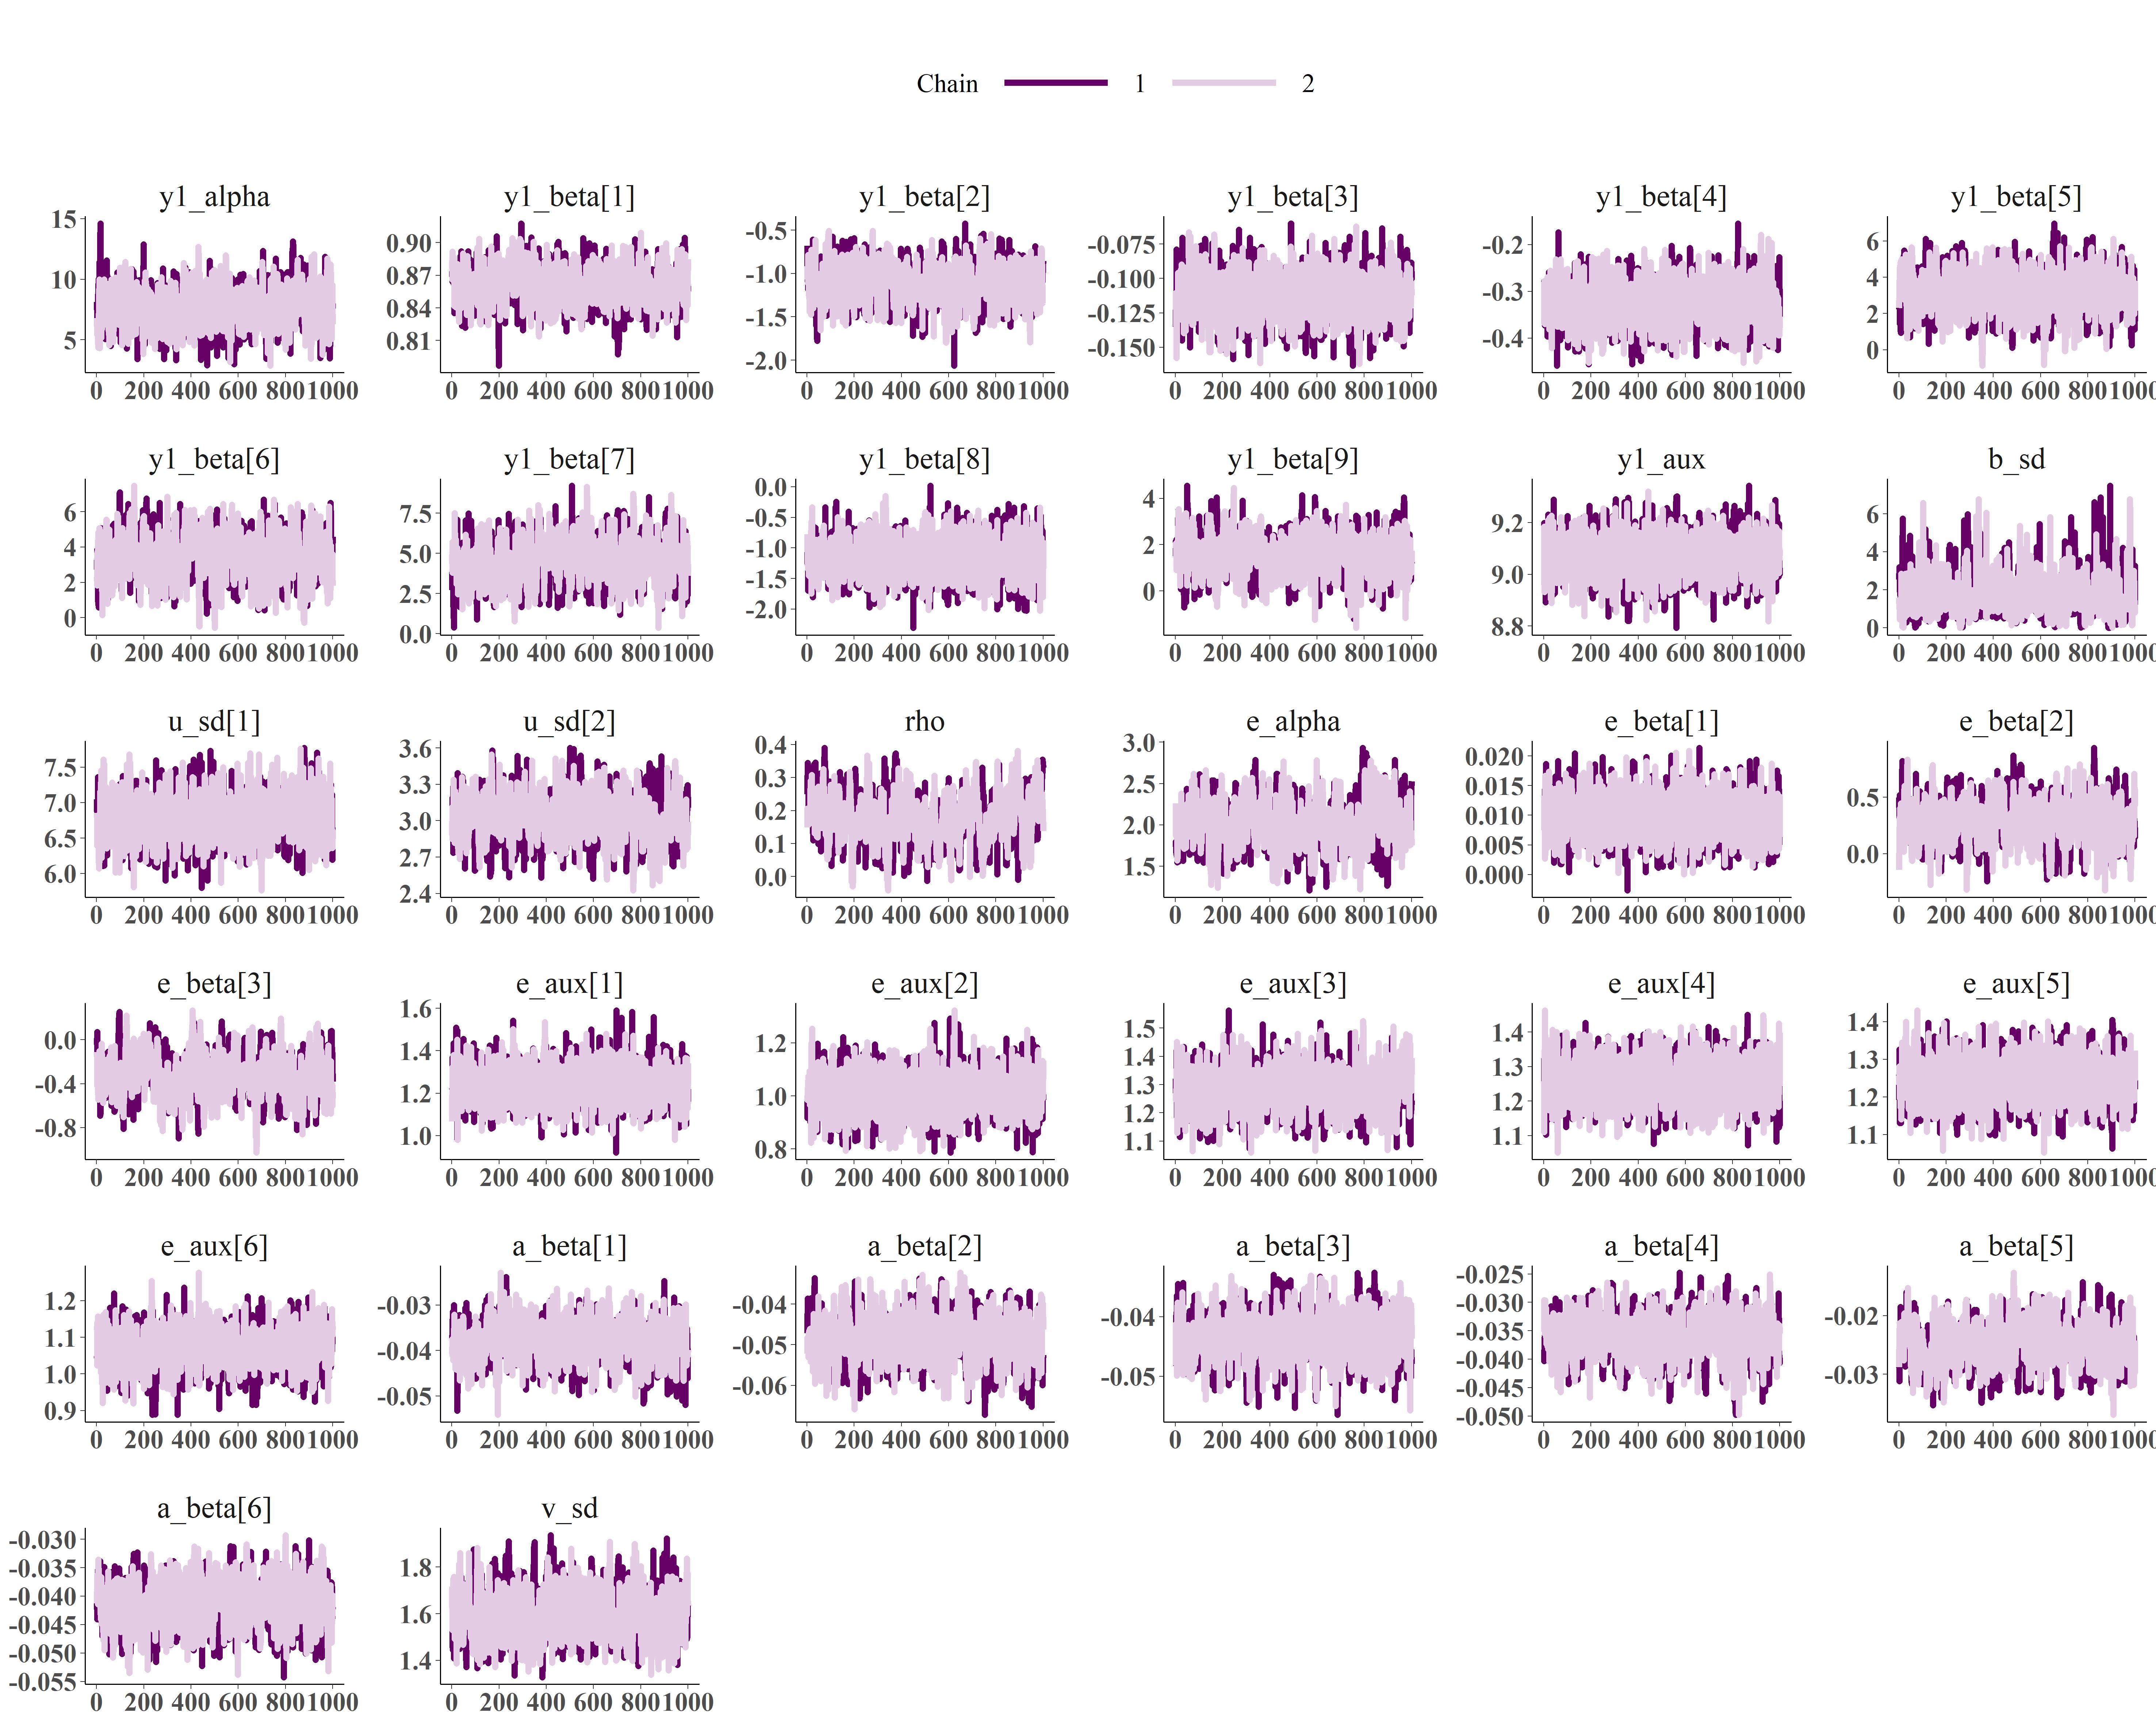
\includegraphics[width=\textwidth]{Figures/Chp3_traceplot.jpg}
\caption{Traceplot against iterations}
\label{fig:trace}
\end{figure}

\begin{figure}[H] 
\centering
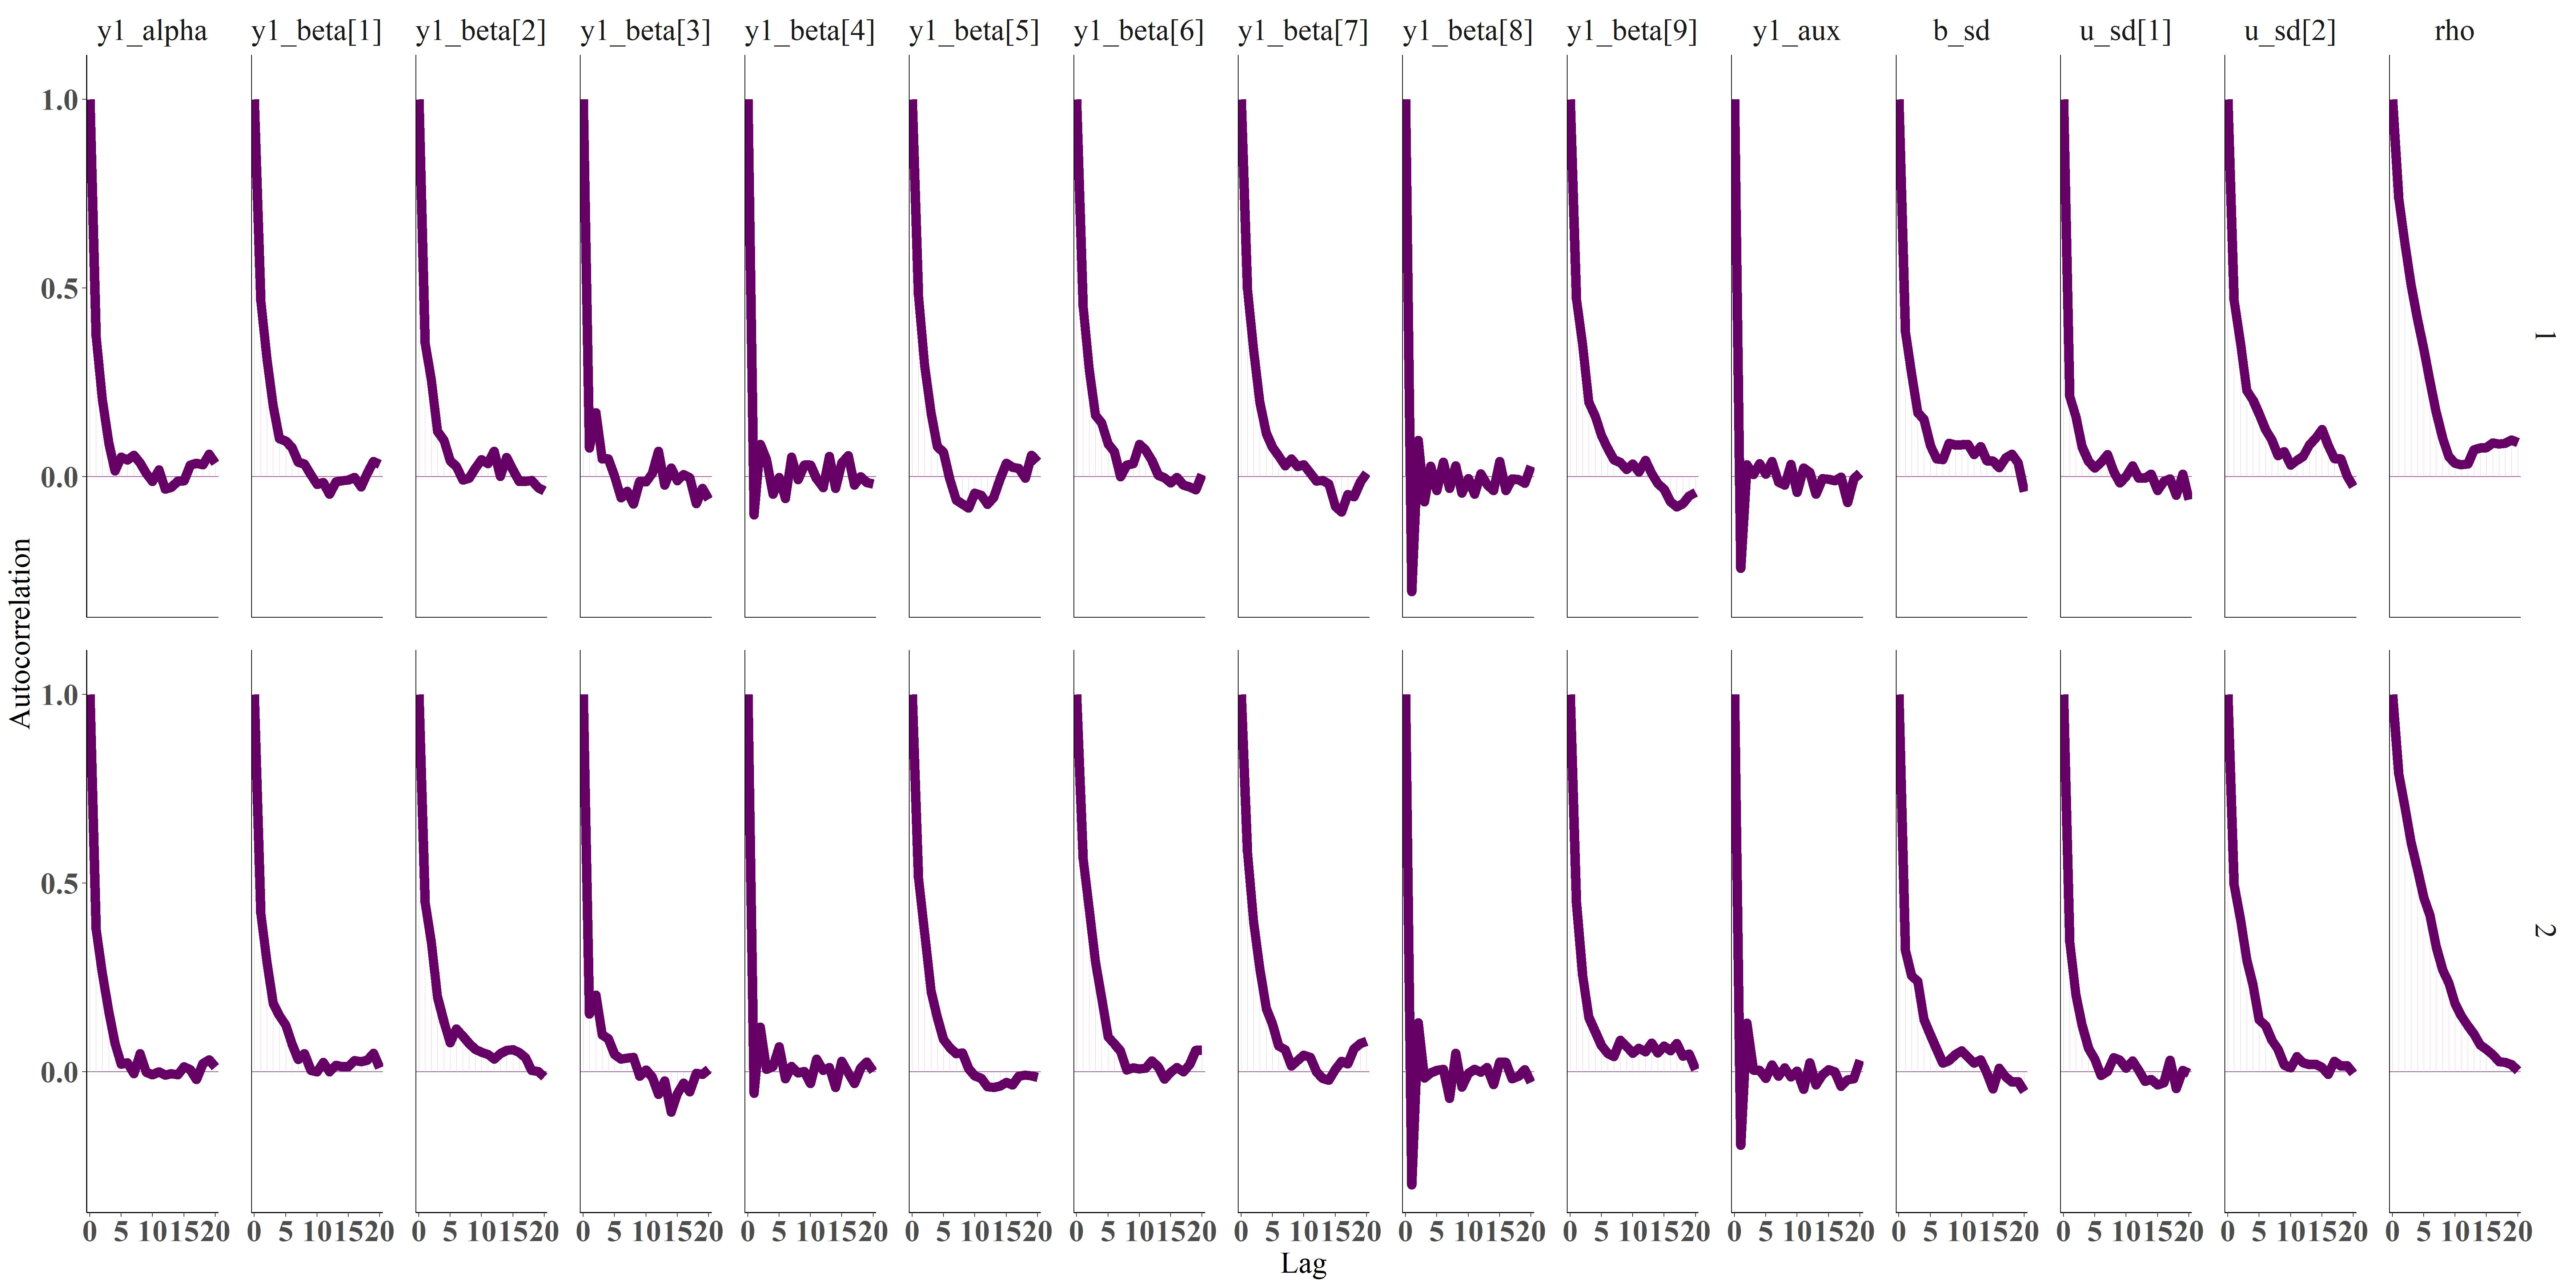
\includegraphics[width=\textwidth]{Figures/Chp3_acf_long.jpg}
\caption{Autocorrelation for parameters from longitudinal submodel}
\label{fig:acf_long}
\end{figure}

\begin{figure}[H] 
\centering
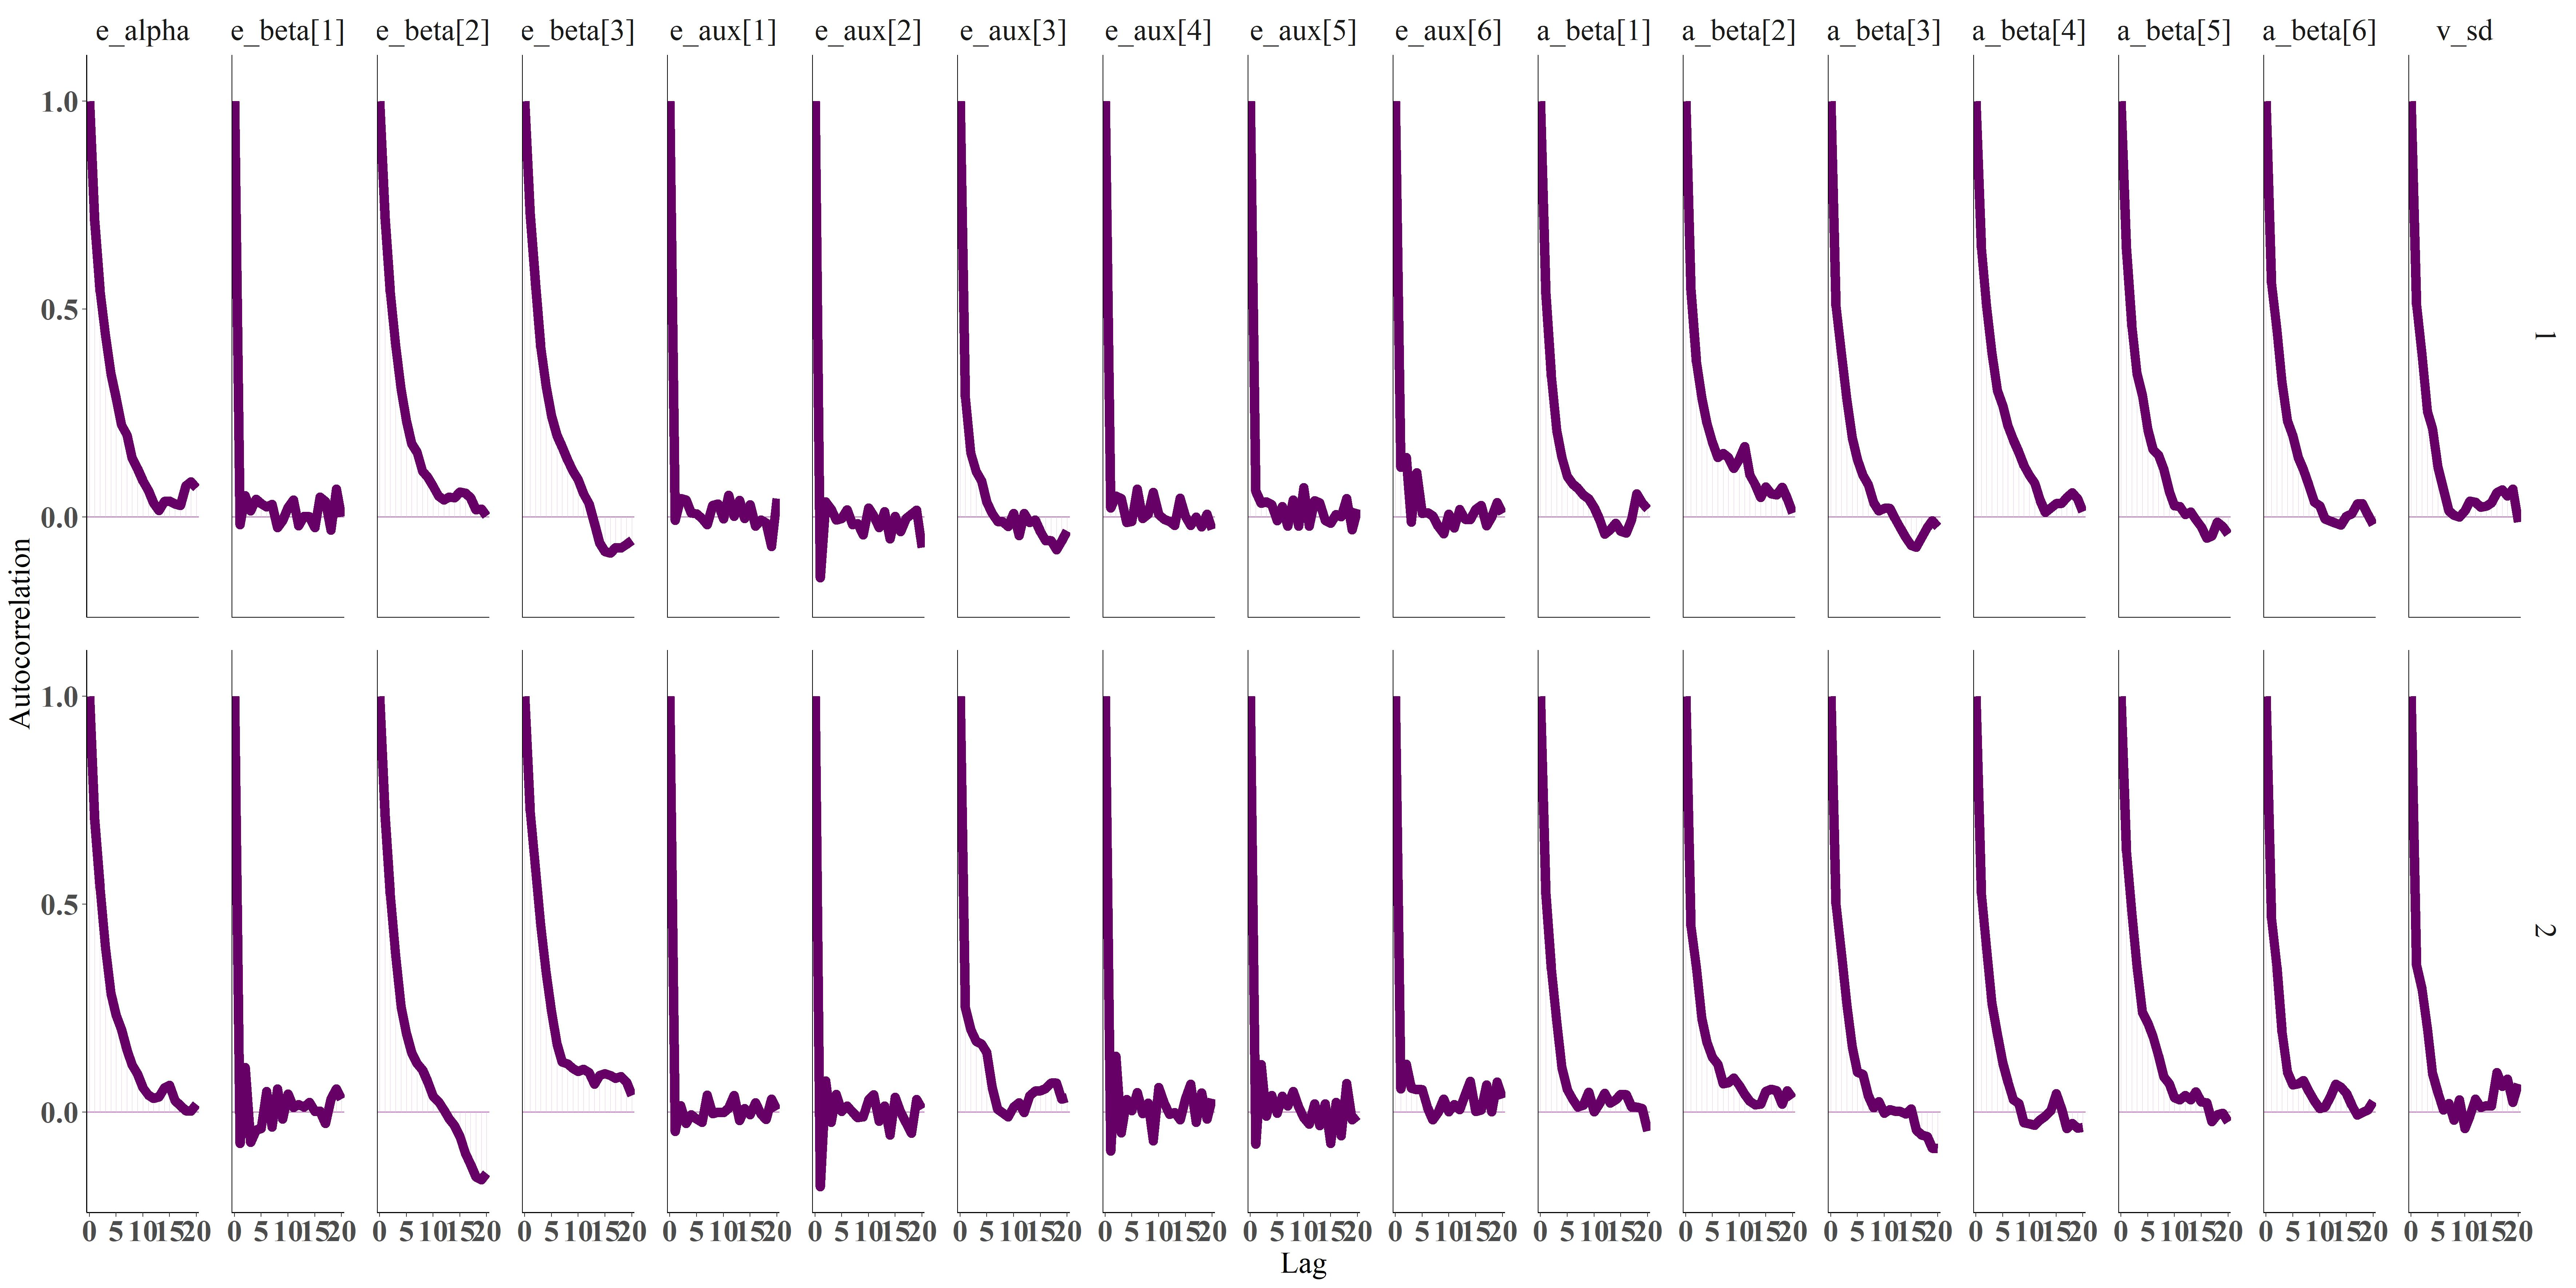
\includegraphics[width=\textwidth]{Figures/Chp3_acf_surv.jpg}
\caption{Autocorrelation for parameters from event submodel}
\label{fig:acf_surv}
\end{figure}


\begin{figure}[H] 
\centering
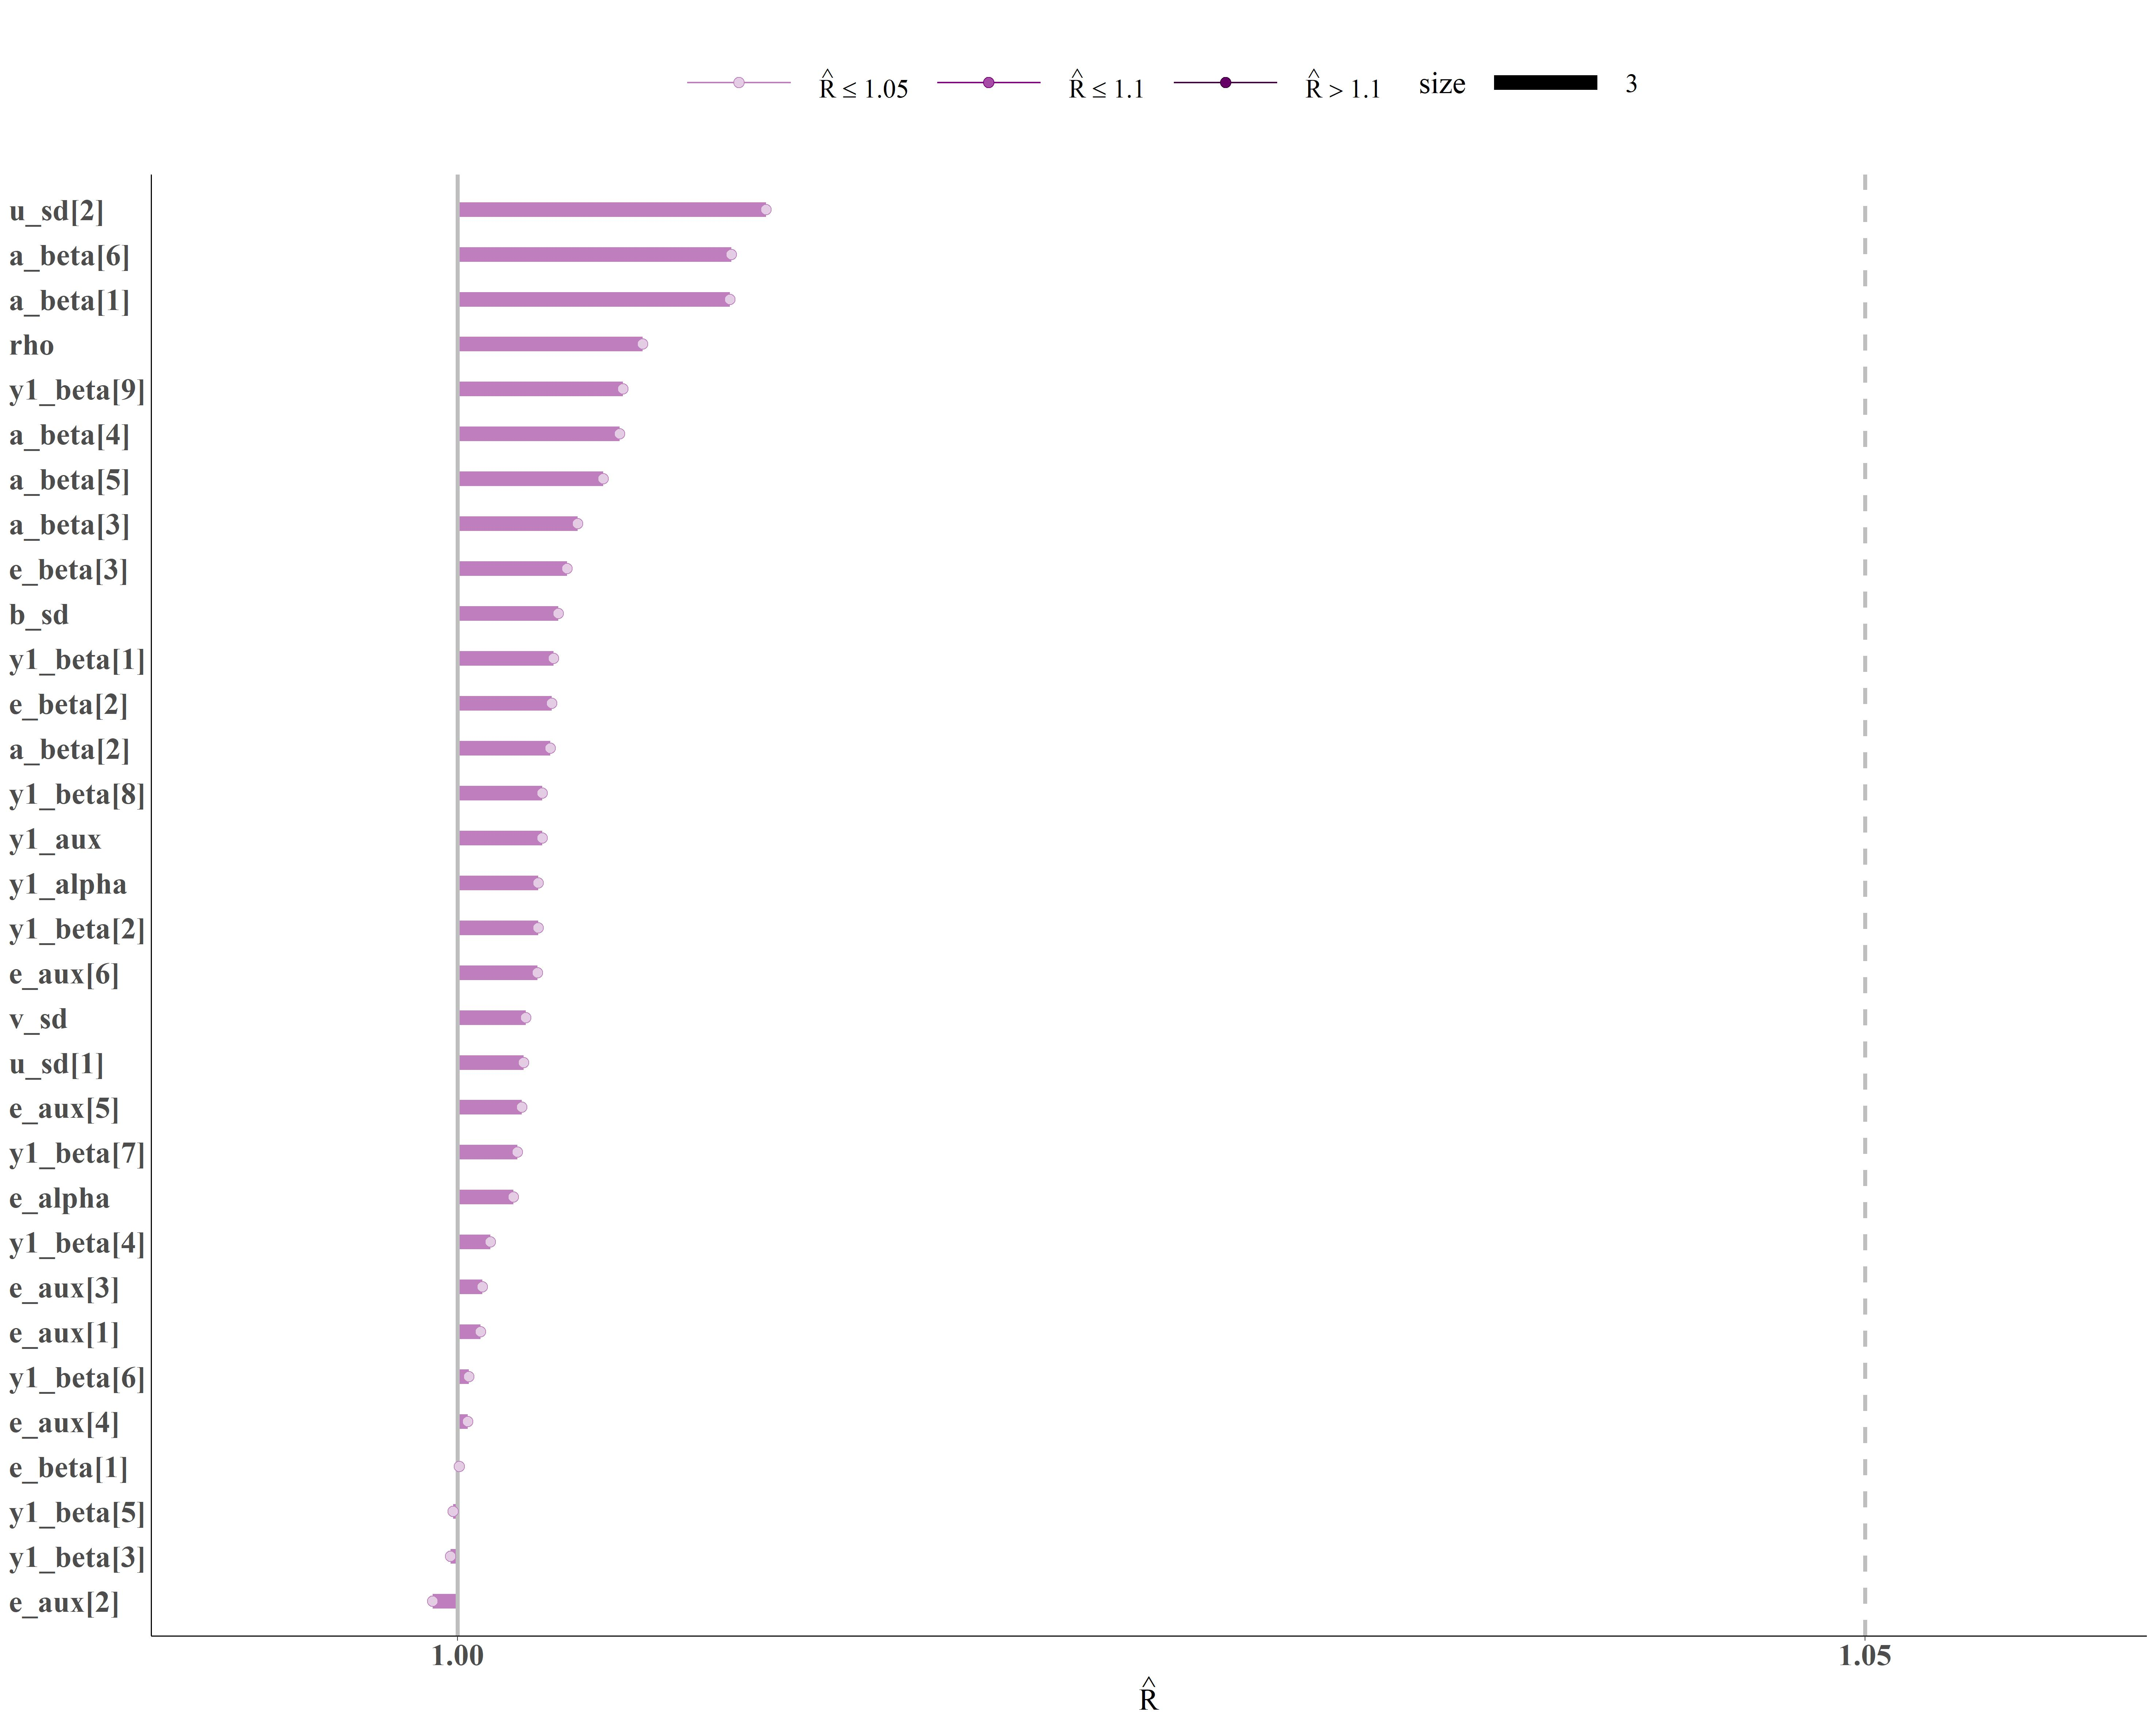
\includegraphics[width=\textwidth]{Figures/Chp3_rhat.jpg}
\caption{Rhat plot}
\label{fig:rhat}
\end{figure}


\section{Time and System}

Additional information about processing system and time are described in Table \ref{tab:system} and Table \ref{tab:time}. All models are estimated with 4000 iterations through two chains. The first 2000 draws are discarded as a warm-up sampling and the remaining 2000 are kept for the posterior inference for both simulated data and real data.

\begin{table}[H] 
\centering
\caption{Processing system}
\begin{tabular}{c|c|c}
\toprule
 & \bf Simulated data & \bf Real data\\
\hline
Platform & x86\_64-apple-darwin17.0 (64-bit) & x86\_64-w64-mingw32/x64 (64-bit)\\
\hline
Running under & macOS Big Sur 10.16 & Windows 10 x64 (build 19043)\\
\hline
R version & 4.0.5 (2021-03-31) & 4.0.2 (2020-06-22) \\
\hline
CmdStan & v2.28.2 & v2.29.1 \\
cmdstanr & v0.4.0 & v0.5.0\\ 
\bottomrule
\end{tabular}
\label{tab:system}
\end{table}


\begin{table}[H] 
  \small\sf\centering
    \caption{\bf Elapsed time in hours across scenarios}
 \begin{threeparttable}
\begin{tabular}{l|l|c|c}
\toprule
Association + Time scale & Model & Simulated data\tnote{a} (N\tnote{b} = 480) & Real data (N\tnote{c} = 440) \\ \hline
\multirow{2}{*}{Slope + Gap} & Joint Model &  0.18 & 9.16\\
                             & Two-stage Model & 0.05 & 2.86\\ \hline
\multirow{2}{*}{Slope + Calendar} & Joint Model & 0.26 & 3.82\\
                                  & Two-stage Model & 0.08 & 2.59 \\ \hline
\multirow{2}{*}{Value + Gap} & Joint Model & 0.18 & 8.17\\ 
                             & Two-stage Model & 0.04 & 5.31 \\ \hline
\multirow{2}{*}{Value + Calendar} & Joint Model & 0.15 & 7.10 \\              
                                           & Two-stage Model & 0.04 & 4.90\\
\bottomrule
\end{tabular}
 \begin{tablenotes}[para]
    \footnotesize
    \item[a] Averaged time per replicate; \item [b] Sample size (number of patients)
    \end{tablenotes}
 \end{threeparttable}
 \label{tab:time}
\end{table}


\section{Example Code}

We attach complete Stan program and partial R code for illustration purpose. For a complete version of R code and simulated data from Github use link: 


\subsection{Stan Program}
\begin{SingleSpace}
    \begin{minted}[breaklines]{R}

/***************************************************/
// Purpose: Fit proposed JM in the manuscript  
// Association structure: Slope/Value
// Risk interval: Gap/Calendar
// Assumption: i) full conditional independence; 
//             ii) LME: random intercept-slope; 
//             iii) Survival: extended stratified relative risk frailty model
// Author: Copyright (C) 2022 Grace C. Zhou
// Date: Mar., 2022
// Based upon:
// Copyright (C) 2015, 2016, 2017 Trustees of Columbia University
// Copyright (C) 2016, 2017 Sam Brilleman

/***************************************************/

functions {

  vector evaluate_eta(matrix X, array[] vector Z_u, int Dev_index,

                      array[] int U_id, array[] int C_id, real gamma,

                      vector beta, vector bVec, matrix uMat) {

    int N = rows(X); // num rows in design matrix

    int K = rows(beta); // num predictors

    //int p = size(Z_u);    // num group level params:intercept+slope

    vector[N] eta;

    if (K > 0) {

      eta = X * beta + gamma * Dev_index;

    } else {

      eta = rep_vector(0.0, N) + gamma * Dev_index;

    }

    //for (k in 1:p)

    for (n in 1 : N) {

      eta[n] = eta[n] + bVec[C_id[n]] * Dev_index

               + uMat[U_id[n], 1] * Z_u[1, n] + uMat[U_id[n], 2] * Z_u[2, n];

    }

    return eta;

  }

  
  /** 

  * Get the indices corresponding to the lower tri of a square matrix

  * @param dim The number of rows in the square matrix

  * @return A vector of indices

  */

  array[] int lower_tri_indices(int dim) {

    array[dim + choose(dim, 2)] int indices;

    int mark = 1;

    for (r in 1 : dim) {

      for (c in r : dim) {

        indices[mark] = (r - 1) * dim + c;

        mark = mark + 1;

      }

    }

    return indices;

  }

}

data {

  //----- Longitudinal submodels

  // population level dimensions

  int<lower=0> y_N; // num observations

  int<lower=0> y_K; // num predictors

  
  // population level data

  vector[y_N] y1; // response vectors

  matrix[y_N, y_K] y1_X; // fix effect design matrix

  vector[y_K] y1_Xbar; // predictor means


  // group level dimensions

  int<lower=0> b_N; // num center

  int<lower=0> b_K; // num center predictor

  int<lower=0> u_N; // num patients

  int<lower=0> u_K;// num patient predictor

  array[y_N] int<lower=0> y1_C_id; // center id 

  array[y_N] int<lower=0> y1_U_id; // patient id 

  array[u_K] vector[y_N] y1_Z; // random effect design matrix


  //----- Event submodel

  // data for calculating event submodel linear predictor in GK quadrature

  // NB these design matrices are evaluated AT the event time and

  // the (unstandardised) quadrature points

  int<lower=0> e_K; // num predictors 

  int<lower=0> a_K; // num assoc params

  int<lower=0> Npat; // num patients (equal to u_N)

  int<lower=0> Nevents; // num events (ie. not censored)

  int<lower=0> qnodes; // num nodes for GK quadrature

  int<lower=0> Nobs_times_qnodes; // Nobs x qnodes

  int<lower=0> nrow_e_Xq; // num rows predictor matrix

  matrix[nrow_e_Xq, e_K] e_Xq; // design matrix 

  vector[e_K] e_Xbar; // predictor means

  real norm_const; // norm constant

  int<lower=0> basehaz_df; // baseline hazard df

  vector[nrow_e_Xq] basehaz_X; // baseline hazard design matrix/vector (basis terms)

  vector[Nobs_times_qnodes] qwts; // GK quadrature weights with (b-a)/2 scaling

  matrix[nrow_e_Xq, y_K] y1_Xq; // fix effect design matrix at quadpoints

  array[u_K] vector[nrow_e_Xq] y1_Zq; // random effect design matrix at quadpoints

  array[nrow_e_Xq] int<lower=0> y1_Cq_id; // center id at quadpoints

  array[nrow_e_Xq] int<lower=0> y1_Uq_id; // patient id at quadpoints

  //----- Hyperparameters for prior distributions

  // scale prior

  vector<lower=0>[y_K] y1_prior_scale;

  vector<lower=0>[e_K] e_prior_scale;

  vector<lower=0>[a_K] a_prior_scale;

  real<lower=0> y_prior_scale_for_intercept;

  real<lower=0> e_prior_scale_for_intercept;

  real<lower=0> y_prior_scale_for_aux;

  vector<lower=0>[basehaz_df] e_prior_scale_for_aux;


  // lkj prior 
  
  real<lower=0> b_prior_scale;

  vector<lower=0>[u_K] u_prior_scale;

  vector<lower=0>[u_K] u_prior_df;

  real<lower=0> u_prior_regularization;

  int<lower=0> Dev_index;

}

transformed data {

  // indexing used to extract lower tri of RE covariance matrix

  array[u_K + choose(u_K, 2)] int u_cov_idx;

  if (u_K > 0) {

    u_cov_idx = lower_tri_indices(u_K);

  }

}

parameters {

 //----- Longitudinal submodel

  real y1_gamma; // intercept 

  vector[y_K] y1_z_beta; // unscaled coef

  real<lower=0> y1_aux_unscaled; // unscaled residual error 

  real<lower=0> b_sd; // center sd

  vector[b_N] z_b_vec; // unscaled center effect 

  matrix[u_K, u_N] z_u_mat; // unscaled patient effect  

  vector<lower=0>[u_K] u_sd; // patient sd  

  cholesky_factor_corr[u_K > 1 ? u_K : 0] u_cholesky; // cholesky factor 
 
 //----- Event submodel

  real e_gamma; // intercept in event submodel

  vector[e_K] e_z_beta; // unscaled log hazard ratio

  vector<lower=0>[basehaz_df] e_aux_unscaled; // unscaled baseline hazard coef

  vector[a_K] a_z_beta; // unscaled assoc params 

  real<lower=0> v_sd; // frailty sd

  vector[Npat] z_v_vec;// unscaled frailty effect

}

transformed parameters {

 //----- Longitudinal submodel
 
  vector[y_K] y1_beta; // scaled coef

  real<lower=0> y1_aux; // scaled residual error 

  matrix[u_N, u_K] u_mat; // patient effect  

  vector[b_N] b_vec; // scaled center effect 

  vector[y_N] y1_eta; // linear predictor 

 //----- Event submodel
 
  vector[nrow_e_Xq] y1_eta_q; // linear predictor at quadpoints

  vector[e_K] e_beta; // scaled coef (log hazard ratio)

  vector[a_K] a_beta; // scaled assoc params 

  vector<lower=0>[basehaz_df] e_aux; // scaled baseline hazard coef

  vector[Npat] v_vec; // scaled frailty effect
  
  //----- Longitudinal submodel 
  
  y1_beta = y1_z_beta .* y1_prior_scale;

  y1_aux = y1_aux_unscaled * y_prior_scale_for_aux;

  b_vec = b_sd * z_b_vec;

  if (u_K == 1) {

    u_mat = (u_sd[1] * z_u_mat)';

  } else if (u_K > 1) {

    u_mat = (diag_pre_multiply(u_sd, u_cholesky) * z_u_mat)';

  }

  //----- Event submodel

  e_beta = e_z_beta .* e_prior_scale;

  a_beta = a_z_beta .* a_prior_scale;

  e_aux = e_aux_unscaled .* e_prior_scale_for_aux;

  v_vec = v_sd * z_v_vec;

  //----- Longitudinal submodel 
  
  // linear predictor at observed time
   
  y1_eta = evaluate_eta(y1_X, y1_Z, 1, y1_U_id, y1_C_id, y1_gamma, y1_beta,

                        b_vec, u_mat);
                        
 //----- Event submodel 
 
 // linear biomarker predictor at event time and quadrature points  

  y1_eta_q = evaluate_eta(y1_Xq, y1_Zq, Dev_index, y1_Uq_id, y1_Cq_id,

                          y1_gamma, y1_beta, b_vec, u_mat);

}

model {

  //---- Longitudinal submodel

  // increment the target with the log-lik

  target += normal_lpdf(y1 | y1_eta, y1_aux);

 //---- Event submodel (Gauss-Kronrod quadrature)

  {

    vector[nrow_e_Xq] e_eta_q; // linear predictor at event time and quadrature points

    vector[nrow_e_Xq] log_basehaz; // log baseline hazard at event time and quadrature points

    vector[nrow_e_Xq] log_haz_q; // log hazard at event time and quadrature points

    vector[Nevents] log_haz_etimes; // log hazard at the event time only

    vector[Nobs_times_qnodes] log_haz_qtimes; // log hazard at the quadrature points only

    for (n in 1 : nrow_e_Xq) {
      
    // Step 1: event submodel add on contribution from association structure to
    // the linear predictor at event time and quadrature points
    
      e_eta_q[n] = e_Xq[n] * e_beta + y1_eta_q[n] * a_beta[y1_Cq_id[n]]

                   + v_vec[y1_Uq_id[n]];

      // Step 2: log baseline hazard (Weibull) at event time and quadrature points

      log_basehaz[n] = e_gamma + norm_const + log(e_aux[y1_Cq_id[n]])

                       + basehaz_X[n] * (e_aux[y1_Cq_id[n]] - 1);

    }

    // Step 3: log hazard at event time and quadrature points

    log_haz_q = log_basehaz + e_eta_q;

    // Step 4: log hazard at event times only

    log_haz_etimes = head(log_haz_q, Nevents);
    
    // Step 5: log hazard at quadrature points only

    log_haz_qtimes = tail(log_haz_q, Nobs_times_qnodes);

    // Step 6: increment the target with the log-lik

    target += sum(log_haz_etimes) - dot_product(qwts, exp(log_haz_qtimes));

  }

  //---- Log-priors

 //----- Longitudinal submodel

  target += normal_lpdf(y1_gamma | 0, y_prior_scale_for_intercept);

  target += normal_lpdf(y1_z_beta | 0, 1);

  target += normal_lpdf(y1_aux_unscaled | 0, 1);

  target += normal_lpdf(z_b_vec | 0, 1);

  target += normal_lpdf(b_sd | 0, b_prior_scale); // following Gelman 2008

  target += student_t_lpdf(u_sd | u_prior_df, 0, u_prior_scale);

  target += normal_lpdf(to_vector(z_u_mat) | 0, 1);

  // corr matrix

  if (u_K > 1) {

    target += lkj_corr_cholesky_lpdf(u_cholesky | u_prior_regularization);

  }

 //----- Event submodel
 
  target += normal_lpdf(e_gamma | 0, e_prior_scale_for_intercept);

  target += normal_lpdf(e_z_beta | 0, 1);

  target += normal_lpdf(a_z_beta | 0, 1);

  target += normal_lpdf(e_aux_unscaled | 0, 1);

  target += normal_lpdf(z_v_vec | 0, 1);

  target += normal_lpdf(v_sd | 0, 10);

}


generated quantities {

  real y1_alpha; // transformed intercept for long submodel

  vector[size(u_cov_idx)] u_cov; // var-cov for patient

  real rho; // correlation coef

  real e_alpha; // transformed intercept for event submodel
  
  //---- Long submodel

  y1_alpha = y1_gamma - dot_product(y1_Xbar, y1_beta);

  // Transform variance-covariance matrix for patient

  if (u_K == 1) {

    u_cov[1] = u_sd[1] * u_sd[1];

  } else {

    u_cov = to_vector(quad_form_diag(multiply_lower_tri_self_transpose(

                                     u_cholesky), u_sd))[u_cov_idx];

  }


  rho = u_cov[2] / (u_sd[1] * u_sd[2]);
  
   for (i in 1 : y_N) {

    log_lik_y[i] = normal_lpdf(y1[i] | y1_eta[i], y1_aux); // log-lik 

    y_tilde[i] = normal_rng(y1_eta[i], y1_aux); // posterior predictive dist

  }

 //---- Event submodel

  e_alpha = e_gamma + norm_const - dot_product(e_Xbar, e_beta);

}


\end{minted}

\subsection{R code}

    \begin{minted}[breaklines]{R}

library(cmdstanr)

file.jm <- file.path("JM.stan")
mod.jm <- cmdstan_model(file.jm)

fit.jm <- mod.jm$sample(
  data = standata.jm,
  chains = 2, 
  save_warmup = FALSE,
  parallel_chains = 2,
  refresh = 500,
  adapt_delta=0.95,
  max_treedepth=12,
  seed=202207,
  init = function() staninit.jm
)

\end{minted}

\end{SingleSpace}


\end{document}
